% -*- Mode:TeX -*-

%% IMPORTANT: The official thesis specifications are available at:
%%            http://libraries.mit.edu/archives/thesis-specs/
%%
%%            Please verify your thesis' formatting and copyright
%%            assignment before submission. If you notice any
%%            discrepancies between these templates and the 
%%            MIT Libraries' specs, please let us know
%%            by e-mailing thesis@mit.edu

%% The documentclass options along with the pagestyle can be used to generate
%% a technical report, a draft copy, or a regular thesis. You may need to
%% re-specify the pagestyle after you \include cover.tex. For more
%% information, see the first few lines of mitthesis.cls. 

%\documentclass[12pt,vi,twoside]{mitthesis}
%%
%%  If you want your thesis copyright to you instead of MIT, use the
%%  ``vi'' option, as above.
%%
%\documentclass[12pt,twoside,leftblank]{mitthesis}
%%
%% If you want blank pages before new chapters to be labelled ``This
%% Page Intentionally Left Blank'', use the ``leftblank'' option, as
%% above. 

\documentclass[12pt,twoside]{mitthesis}
\usepackage{lgrind}
\usepackage{booktabs}
%% These have been added at the request of the MIT Libraries, because
%% some PDF conversions mess up the ligatures.  -LB, 1/22/2014
\usepackage{cmap}
\usepackage[T1]{fontenc}
\pagestyle{plain}

% ABF custom packages
\usepackage{xcolor}
\usepackage{graphicx}
\usepackage{float}
\usepackage{subcaption}
\usepackage{hyperref}
\usepackage{amssymb}
\newcommand\todo[1]{\textcolor{red}{#1}}

%% This bit allows you to either specify only the files which you wish to
%% process, or `all' to process all files which you \include.
%% Krishna Sethuraman (1990).

%\typein [\files]{Enter file names to process, (chap1,chap2 ...), or `all' to process all files:}
\def\all{all}
\ifx\files\all \typeout{Including all files.} \else %\typeout{Including only \files.} \includeonly{\files} \fi

\begin{document}

% -*-latex-*-
% 
% For questions, comments, concerns or complaints:
% thesis@mit.edu
% 
%
% $Log: cover.tex,v $
% Revision 1.9  2019/08/06 14:18:15  cmalin
% Replaced sample content with non-specific text.
%
% Revision 1.8  2008/05/13 15:02:15  jdreed
% Degree month is June, not May.  Added note about prevdegrees.
% Arthur Smith's title updated
%
% Revision 1.7  2001/02/08 18:53:16  boojum
% changed some \newpages to \cleardoublepages
%
% Revision 1.6  1999/10/21 14:49:31  boojum
% changed comment referring to documentstyle
%
% Revision 1.5  1999/10/21 14:39:04  boojum
% *** empty log message ***
%
% Revision 1.4  1997/04/18  17:54:10  othomas
% added page numbers on abstract and cover, and made 1 abstract
% page the default rather than 2.  (anne hunter tells me this
% is the new institute standard.)
%
% Revision 1.4  1997/04/18  17:54:10  othomas
% added page numbers on abstract and cover, and made 1 abstract
% page the default rather than 2.  (anne hunter tells me this
% is the new institute standard.)
%
% Revision 1.3  93/05/17  17:06:29  starflt
% Added acknowledgements section (suggested by tompalka)
% 
% Revision 1.2  92/04/22  13:13:13  epeisach
% Fixes for 1991 course 6 requirements
% Phrase "and to grant others the right to do so" has been added to 
% permission clause
% Second copy of abstract is not counted as separate pages so numbering works
% out
% 
% Revision 1.1  92/04/22  13:08:20  epeisach

% NOTE:
% These templates make an effort to conform to the MIT Thesis specifications,
% however the specifications can change. We recommend that you verify the
% layout of your title page with your thesis advisor and/or the MIT 
% Libraries before printing your final copy.
\title{Microarchitecture Categorization and Pre-RTL Analytical Modeling for Sparse Tensor Accelerators}

\author{Andrew Feldman}
% If you wish to list your previous degrees on the cover page, use the 
% previous degrees command:
\prevdegrees{S.B. in Electrical Engineering and Computer Science \\ Massachusetts Institute of Technology (2016)}
% You can use the \\ command to list multiple previous degrees
%       \prevdegrees{B.S., University of California (1978) \\
%                    S.M., Massachusetts Institute of Technology (1981)}
\department{Department of Electrical Engineering and Computer Science}

% If the thesis is for two degrees simultaneously, list them both
% separated by \and like this:
% \degree{Doctor of Philosophy \and Master of Science}
\degree{Master of Engineering in Electrical Engineering and Computer Science}

% As of the 2007-08 academic year, valid degree months are September, 
% February, or June.  The default is June.
\degreemonth{February}
\degreeyear{2024}
\thesisdate{\today}

%% By default, the thesis will be copyrighted to MIT.  If you need to copyright
%% the thesis to yourself, just specify the `vi' documentclass option.  If for
%% some reason you want to exactly specify the copyright notice text, you can
%% use the \copyrightnoticetext command.  
%\copyrightnoticetext{\copyright IBM, 1990.  Do not open till Xmas.}

% If there is more than one supervisor, use the \supervisor command
% once for each.
\supervisor{Vivienne Sze}{Associate Professor}
\supervisor{Joel Emer}{Professor of the Practice}

% This is the department committee chairman, not the thesis committee
% chairman.  You should replace this with your Department's Committee
% Chairman.
\chairman{Katrina LaCurts}{Chair, Master of Engineering Thesis Committee}

% Make the titlepage based on the above information.  If you need
% something special and can't use the standard form, you can specify
% the exact text of the titlepage yourself.  Put it in a titlepage
% environment and leave blank lines where you want vertical space.
% The spaces will be adjusted to fill the entire page.  The dotted
% lines for the signatures are made with the \signature command.
\maketitle

% The abstractpage environment sets up everything on the page except
% the text itself.  The title and other header material are put at the
% top of the page, and the supervisors are listed at the bottom.  A
% new page is begun both before and after.  Of course, an abstract may
% be more than one page itself.  If you need more control over the
% format of the page, you can use the abstract environment, which puts
% the word "Abstract" at the beginning and single spaces its text.

%% You can either \input (*not* \include) your abstract file, or you can put
%% the text of the abstract directly between the \begin{abstractpage} and
%% \end{abstractpage} commands.

% First copy: start a new page, and save the page number.
\cleardoublepage
% Uncomment the next line if you do NOT want a page number on your
% abstract and acknowledgments pages.
% \pagestyle{empty}
\setcounter{savepage}{\thepage}
\begin{abstractpage}
% $Log: abstract.tex,v $
% Revision 1.1  93/05/14  14:56:25  starflt
% Initial revision
% 
% Revision 1.1  90/05/04  10:41:01  lwvanels
% Initial revision
% 
%
%% The text of your abstract and nothing else (other than comments) goes here.
%% It will be single-spaced and the rest of the text that is supposed to go on
%% the abstract page will be generated by the abstractpage environment.  This
%% file should be \input (not \include 'd) from cover.tex.

% , utilizing simple formulae for \textit{architectural} compute and memory savings from sparse acceleration features (SAFs.) 

Specialized microarchitectures for exploiting sparsity have critical to the design of sparse tensor accelerators. Despite considerable research having been done, prior work lacks consistent abstractions, systematic design-space exploration, and apples-to-apples comparison between alternative microarchitecture proposals.

Sparseloop (in combination with the Accelergy modeling framework) is an example of an existing tool which attempts to analytically model sparsity optimizations, known as Sparse Acceleration Features (SAFs.) Sparseloop effectively models key metrics such as energy, area and cycles at the architecture-level in the presence of sparsity optimizations. However, lacking models of microarchitectural primitives and design topologies, Sparseloop is unable to lower its sparsity abstractions onto a model of microarchitectural costs. Thus Sparseloop cannot capture the energy/area/time overhead incurred by SAF microarchitectures.

This work attempts to synthesize a number of prior works into a concise, unified, and effective framework for doing research on SAF microarchitectures. This overall framework comprises (1) a conceptual framework which facilitates concise description and design-space exploration for SAF microarchitectures, (2) a software framework for compiling Sparseloop-style SAF descriptions into microarchitecture designs and analytical models, and (3) a component library including specific SAF microarchitecture subcomponent designs as well as RTL to support implementation. 
\end{abstractpage}

% Additional copy: start a new page, and reset the page number.  This way,
% the second copy of the abstract is not counted as separate pages.
% Uncomment the next 6 lines if you need two copies of the abstract
% page.
% \setcounter{page}{\thesavepage}
% \begin{abstractpage}
% % $Log: abstract.tex,v $
% Revision 1.1  93/05/14  14:56:25  starflt
% Initial revision
% 
% Revision 1.1  90/05/04  10:41:01  lwvanels
% Initial revision
% 
%
%% The text of your abstract and nothing else (other than comments) goes here.
%% It will be single-spaced and the rest of the text that is supposed to go on
%% the abstract page will be generated by the abstractpage environment.  This
%% file should be \input (not \include 'd) from cover.tex.

% , utilizing simple formulae for \textit{architectural} compute and memory savings from sparse acceleration features (SAFs.) 

Specialized microarchitectures for exploiting sparsity have critical to the design of sparse tensor accelerators. Despite considerable research having been done, prior work lacks consistent abstractions, systematic design-space exploration, and apples-to-apples comparison between alternative microarchitecture proposals.

Sparseloop (in combination with the Accelergy modeling framework) is an example of an existing tool which attempts to analytically model sparsity optimizations, known as Sparse Acceleration Features (SAFs.) Sparseloop effectively models key metrics such as energy, area and cycles at the architecture-level in the presence of sparsity optimizations. However, lacking models of microarchitectural primitives and design topologies, Sparseloop is unable to lower its sparsity abstractions onto a model of microarchitectural costs. Thus Sparseloop cannot capture the energy/area/time overhead incurred by SAF microarchitectures.

This work attempts to synthesize a number of prior works into a concise, unified, and effective framework for doing research on SAF microarchitectures. This overall framework comprises (1) a conceptual framework which facilitates concise description and design-space exploration for SAF microarchitectures, (2) a software framework for compiling Sparseloop-style SAF descriptions into microarchitecture designs and analytical models, and (3) a component library including specific SAF microarchitecture subcomponent designs as well as RTL to support implementation. 
% \end{abstractpage}

\cleardoublepage

\section*{Acknowledgments}

Special thanks to Dr. Nellie Wu, Professor Vivienne Sze, and Professor Joel Emer for their support during the development of this thesis. 

The textual content of this thesis document was written by the Author without the aid of ChatGPT or other tools.
 
ChatGPT was used to accelerate boilerplate or tedious coding tasks such as writing file parsing and plotting code, unrolling scalar RTL into a vectorized implementation, writing testbenches, and generating visualizations or tabulations of experimental results. All AI generated outputs were manually and thoroughly checked for correctness before being used in experiments. 

The core contributions of this work – development of a microarchitecture taxonomy, development of microarchitecture modeling principles, software architecture, and the vast majority of the software development - were original and completed entirely by the Author, without the aid of AI.

%%%%%%%%%%%%%%%%%%%%%%%%%%%%%%%%%%%%%%%%%%%%%%%%%%%%%%%%%%%%%%%%%%%%%%
% -*-latex-*-

% Some departments (e.g. 5) require an additional signature page.  See
% signature.tex for more information and uncomment the following line if
% applicable.
% % -*- Mode:TeX -*-
%
% Some departments (e.g. Chemistry) require an additional cover page
% with signatures of the thesis committee.  Please check with your
% thesis advisor or other appropriate person to determine if such a 
% page is required for your thesis.  
%
% If you choose not to use the "titlepage" environment, a \newpage
% commands, and several \vspace{\fill} commands may be necessary to
% achieve the required spacing.  The \signature command is defined in
% the "mitthesis" class
%
% The following sample appears courtesy of Ben Kaduk <kaduk@mit.edu> and
% was used in his June 2012 doctoral thesis in Chemistry. 

\begin{titlepage}
\begin{large}
This doctoral thesis has been examined by a Committee of the Department
of Chemistry as follows:

\signature{Professor Jianshu Cao}{Chairman, Thesis Committee \\
   Professor of Chemistry}

\signature{Professor Troy Van Voorhis}{Thesis Supervisor \\
   Associate Professor of Chemistry}

\signature{Professor Robert W. Field}{Member, Thesis Committee \\
   Haslam and Dewey Professor of Chemistry}
\end{large}
\end{titlepage}


\pagestyle{plain}
  % -*- Mode:TeX -*-
%% This file simply contains the commands that actually generate the table of
%% contents and lists of figures and tables.  You can omit any or all of
%% these files by simply taking out the appropriate command.  For more
%% information on these files, see appendix C.3.3 of the LaTeX manual. 
\tableofcontents
\newpage
\listoffigures
\newpage
\listoftables


%% This is an example first chapter.  You should put chapter/appendix that you
%% write into a separate file, and add a line \include{yourfilename} to
%% main.tex, where `yourfilename.tex' is the name of the chapter/appendix file.
%% You can process specific files by typing their names in at the 
%% \files=
%% prompt when you run the file main.tex through LaTeX.
\chapter{Introduction}
\label{chapter:introduction}

Accelerating tensor operations is a significant research area with applications in deep neural network (DNN)-based machine learning inference\cite{eyeriss}\cite{eyerissv2}\cite{tpu}\cite{extensor}, scientific computing\cite{sci_tensor}, graph analytics\cite{mattson2013standards}, and data science\cite{mcauley2013hidden}\cite{kolda2009tensor}\cite{bader2008discussion}. Industrial demand for large scale\cite{tpu} and/or energy-efficient\cite{eyeriss} DNN deployment, combined with the demise of Moore's Law\cite{moore}, motivated the first generation of DNN-oriented tensor accelerators\cite{eyeriss}\cite{tpu}.

More recently, a new generation of hardware accelerators exploit tensor sparsity for improved scalability and efficiency\cite{ampere}\cite{eyerissv2}\cite{sparten}\cite{sparch}\cite{scnn}\cite{candles}\cite{extensor}. Tensor zero-compression \cite{szebook} \cite{sparseloop} \cite{extensor} and data-dependent computation strategies such as gating and skipping \cite{szebook} \cite{sparseloop} can meaningfully impact memory footprint, energy, area and total cycle time of an accelerator computation\cite{szebook}\cite{sparseloop}.

By removing elements, tensor zero-compression removes the regular structure that makes trivial operations such as iteration and co-iteration through tensor ranks feasible. While this problem is resolved with a layer of indirection (i.e. by adding \textit{metadata} that can recover the original coordinates of non-zero elements\cite{szebook}), the resulting sparse-tensor versions of these operations are sometimes more complex and resource intensive than their dense tensor counterparts\cite{extensor}\cite{sparten}\cite{sparch}\cite{ampere}. 

An additional avenue for exploiting sparsity is to optimize away arithmetic operations \cite{eyerissv2} \cite{sparten}\cite{extensor} \cite{sparch} \cite{szebook} \cite{sparseloop} (or quiesce compute during ineffectual operations (IneffOps)\cite{eyeriss}\cite{sparseloop}\cite{szebook}), the cost being a more complex microarchitecture that implements the sparsity-optimized arithmetic\cite{eyeriss}\cite{eyerissv2}. Generally speaking, to exploit sparsity for gains on key metrics, and still create a functionally correct accelerator, researchers frequently are compelled to specialize traversal\cite{szebook}\cite{extensor}, contraction\cite{gamma}\cite{eyerissv2}\cite{extensor}\cite{sparten}, or transposition/shuffle\cite{gamma} microarchitectures to be compatible with the architecture and its sparse representation format(s). Sometimes sparsity creates the need for microarchitectural functions that an equivalent dense tensor accelerator might not require for a similar workload, such as managing memory conflicts\cite{scnn}\cite{sparten}. New specialized microarchitectures for exploiting sparsity have played a key role in the advancement of sparse tensor accelerator research\cite{gamma}\cite{outerspace}\cite{extensor}\cite{sparch}\cite{outerspace}\cite{ampere}.

The Sparseloop\cite{sparseloop} paper introduced the Sparse Acceleration Feature (SAF) abstraction, which unifies prior work on sparse tensor accelerators into a taxonomy of sparsity optimizations. In addition to the SAF abstraction, Sparseloop\cite{sparseloop} also introduced a sparsity extension for Timeloop\cite{timeloop}, a pre-existing architectural modeling tool for dense tensor accelerators. 

Timeloop relies on a consistent set of abstractions for common architectural blocks, i.e. MAC, network-on-chip (NoC), Buffer (which can be subclassed as SRAM, DRAM, register file, ...), etc. Timeloop is used alongside Accelergy\cite{accelergy}, a pre-RTL analytical modeling framework, in order to associate architectural blocks with analytical energy/area models. 

Sparseloop incorporates the SAF abstraction into Timeloop\cite{sparseloop}. The user may specify one or more SAFs, and designate which architectural components (buffers, arithmetic) the SAFs are bound to. To estimate energy savings for a SAF optimization, the idealized SAF is lowered to align with the architectural component model it applies to, resulting in a decrease in the number of actions against that architectural component, and/or an adjustment to memory footprint and memory bandwidth utilization which accounts for sparse tensor representation formats. Broadly speaking, Sparseloop estimates the impact of SAF optimizations on architectural energy and area metrics.

Recall that sparse representation formats may increase the complexity of otherwise trivial operations. Architects of dense tensor accelerators might treat as insignificant the energy and area overhead incurred by SAF implementations, however Section~\ref{chapter:background} will show that as a proportion of total design area, the overhead costs of microarchitectures which implement SAFs (hereafter \textit{SAF microarchitectures}) \textit{may or may not} be very significant. This would suggest that SAF microarchitecture modeling is potentially critical: any benefit a SAF offers for architectural energy/area metrics, could in principle be offset by the energy/area overhead of the SAF microarchitecture.

In theory, Sparseloop could solve the SAF microarchitecture modeling issue, by lowering each SAF to align with a model of SAF microarchitecture energy-per-action and area, yielding an estimate of how the microarchitectural cost of the optimization trades off against its benefit in reducing architectural energy consumption. In practice, Sparseloop lacks abstractions or analytical models of SAF microarchitectural primitives and design topologies. When it comes to design-space exploration, SAF microarchitectures are neither factored into the computation energy estimate, nor into the accelerator area estimate.

Accelerator architectures benefit from tools like Timeloop and Sparseloop which facilitate design-space exploration and apples-to-apples comparison between accelerator designs. A framework of abstractions and models for SAF microarchitectures could increase the accuracy of cost comparisons between sparse tensor accelerators, and increase the likelihood that design-space exploration yields a sparse tensor accelerator that has low cost in practice.

This work attempts to synthesize a number of prior works into a concise, unified, and effective framework for doing research on SAF microarchitectures. The overall framework developed here comprises (1) a conceptual framework which facilitates concise description, modeling and design-space exploration for SAF microarchitectures, (2) a software framework, SAFTools, for compiling Sparseloop-style SAF descriptions into microarchitecture designs and analytical models, and (3) an extensible component library including specific SAF microarchitecture subcomponent designs as well as RTL to support implementation. SAFTools yields pre-RTL analytical models which are compatible with Accelergy and Sparseloop, and which hook into Accelergy architectural buffer models in such a way, that architectural buffer actions are translated into actions against a model of SAF microarchitecture energy. Furthermore, SAF microarchitecture area is factored into total design area. 

As a first step toward a set of consistent abstractions and modeling tools for SAF microarchitecture primitives - analogous to what is currently available for architectural modeling - it is hoped that this work will help enable researchers to systematically explore and compare sparsity optimizations in the design of sparse tensor accelerators. Section~\ref{chapter:background} provides background on SAF microarchitecture research and why it matters. Section~\ref{chapter:conceptual_framework} builds a novel conceptual framework for describing SAF microarchitectures. Section~\ref{chapter:rtl} overviews the RTL component designs (``RTL blocks'') which were written and characterized in order to support model development (additionally, these RTL blocks comprise the RTL library associated with this work.) Section~\ref{chapter:modeling} introduces abstractions for workload modeling, which aid in decoupling dataflow from SAF microarchitecture. Section~\ref{chapter:primitive_taxo_model} introduces the taxonomy of SAF microarchitecture primitives. Building on the previous section, Section~\ref{chapter:saf_microarchitectures} introduces the taxonomy of high-level SAF microarchitecture compound component blocks. Section~\ref{chapter:framework} overviews the architecture of the SAFtools software, component libraries, and RTL block libraries. Section~\ref{chapter:evaluation} evaluates some of SAFTools' capabilities. Section~\ref{chapter:case_studies} provides a case-study of using SAFTools to help design a sparse tensor accelerator with SIMD arithmetic.

%\begin{table}[ht]
%\resizebox{\textwidth}{!}{%
%\begin{tabular}{c|p{2.5cm}|p{2.5cm}|p{2.5cm}|p{2.5cm}}
% & Modeling speed & Accurate SAF $\mu$architecture modeling & Consistent SAF $\mu$architecture abstractions? & Open-source SAF $\mu$architecture RTL?\\ \hline \hline
%Architectural modeling frameworks & \textcolor{green}{\textbf{Fast}} & \textcolor{red}{\textbf{No}} & \textcolor{red}{\textbf{No}} & \textcolor{red}{\textbf{No}} \\ \hline
%Design-specific models & \textcolor{red}{\textbf{Slow}} & \textcolor{green}{\textbf{Yes}} & \textcolor{red}{\textbf{No}} & \textcolor{red}{\textbf{Limited}} \\ \hline
%$\mu$architecture taxonomy papers & \textcolor{red}{\textbf{N/A}} & \textcolor{red}{\textbf{No}} & \textcolor{red}{\textbf{Limited}} & \textcolor{red}{\textbf{No}} \\ \hline
%\textbf{This work} & \textcolor{green}{\textbf{Fast}} & \textcolor{green}{\textbf{Yes}} & \textcolor{green}{\textbf{Yes}} & \textcolor{green}{\textbf{Yes}} \\ \hline
%\end{tabular}
%}
%\label{tab:thiswork}
%\caption{SAFTools and the underlying SAF microarchitecture taxonomy enable fast, accurate SAF microarchitecture modeling based on a consistent set of abstractions.}
%\centering
%\end{table}
\chapter{Background and motivation}
\label{chapter:background}

Sparseloop\cite{sparseloop} developed a unified taxonomy of Sparse Acceleration Features (SAFs), architectural optimization strategies for exploiting sparsity (zero-sparsity) to conserve energy and cycles. A SAF is a strictly declarative description of an optimization, comprising (1) a description of the optimization outcome, and (2) a set of attributes which modulate the outcome of the optimization. A SAF describes neither the microarchitectural implementation of the optimization, nor the interfaces or communication protocols involved in integrating the microarchitectural implementation into the design. 

Nonetheless, a real design would require a microarchitectural change which implements the optimization, referred to here as the \textit{SAF microarchitecture.} Existing analytical modeling tools\cite{sparseloop} model only the benefits of exploiting SAFs (savings on memory capacity, fewer memory accesses, fewer compute cycles); these benefits are introduced in Section~\ref{background:safs}. These tools avoid modeling the costs of SAF microarchitectures by assuming (1) an ideal SAF microarchitecture which perfectly implements the SAF, and (2) a SAF microarchitecture with negligible energy and area overhead.

Section~\ref{background:saf_uarch} demonstrates that SAF microarchitectures can \textit{sometimes} have significant implications for the design and modeling of sparse tensor accelerators. Thus, this work is motivated by the need to create novel SAF microarchitecture models.
%
% SAFs subsection
%
\section{SAFs}
\label{background:safs}

This section will review and motivate the two broad SAF categories. Table~\ref{tab:design_specific_models} provides examples of how SAFs are used in prior research.

%
% Figure: examples of action optimizations
%
\begin{figure*}[h]
\includegraphics[width=\textwidth]{figures/saf_action_optimizations.PNG}
\caption{An example of dot-product optimized with zero-gating and zero-skipping to save cycles and energy, versus the naive un-optimized approach. The zero-skipping optimization's efficacy may depend on the choice of leader-follower skipping vs bidirectional skipping.}
\label{fig:saf_action_optimizations}
\end{figure*}
%
% Table: Action SAFs, comparison of perf and energy
%
\begin{table*}[ht]
\begin{tabular}{c|c|c|}
 & Cycles & Energy \\ \hline \hline
Theoretical &  \textcolor{green}{\textbf{1}} & \textcolor{green}{\textbf{$E_{mac}$}}\\ \hline
Naive &  \textcolor{red}{\textbf{5}} & \textcolor{red}{\textbf{$5 E_{mac}$}}\\ \hline
Zero-gating &  \textcolor{red}{\textbf{5}} & \textcolor{green}{\textbf{$E_{mac}$}} \\ \hline
Zero-skipping (leader-follower) & \textcolor{red}{\textbf{2}} & \textcolor{red}{\textbf{$2 E_{mac}$}} \\ \hline
Zero-skipping (bidirectional) & \textcolor{green}{\textbf{1}} & \textcolor{green}{\textbf{$E_{mac}$}} \\ \hline
\end{tabular}
\caption{Dot-product cycles and energy with different action-optimization strategies applied to the PE in Figure \ref{fig:saf_action_optimizations}, versus the theoretical-best. Energy is measured in multiples of the energy of a single MAC, $E_{mac}$}
\label{tab:action_saf_comparison}
\centering
\end{table*}
%
% Content: SAFs
%

%
\todo{impact on memory; more concise - table shows memory and mac energy, paragraph concisely introduces each action optimization. Clarify that skipping is architecturally one or both operands being skipped in response to the other.}


\subsection{Action optimizations}

These are SAFs which signify that the tensor accelerator detects and optimizes away ineffectual operations such as $0 \times 0 = 0$ and $0 \times a = 0$, with the goal of saving energy and potentially compute cycles. Figure \ref{fig:saf_action_optimizations} compares action optimization cost for a dot-product problem mapped to a simple PE with two buffers and a MAC unit which consumes $E_{mac}$ per operation. Theoretically only one cycle and $E_{mac}$ energy should be required to multiply $a_0 \times b_0$; there are no other effectual MAC operations. Table \ref{tab:action_saf_comparison} shows that a "naive" PE design with no action optimization SAFs underperforms on both cycles and energy by $5\times$, and Figure \ref{fig:saf_action_optimizations} shows that the cause is ineffectual MACs being performed. \textit{Zero-gating} (or \textit{gating}) conserves $E_{mac}$ energy per ineffectual MAC since the MAC unit idles for a cycle. In other words there is no conservation of cycles for ineffectual operations, only energy. \textit{Zero-skipping} (or \textit{skipping}) conserves $E_{mac}$ per ineffectual MAC, but does so by skipping immediately to the next one - thus both energy and time are saved by skipping. 

Designs with \textit{bidirectional action optimizations} do not perform a MAC when either operand is zero. Thus 100\% of gating or skipping opportunities are exploited, depending on the type of action optimization. Designs with \textit{leader-follower action optimizations} respond only to the designated leader operand being zero, in which case both the MAC and the follower memory access are skipped or gated.

Figure~\ref{todo} summarizes the attributes of action optimizations. The key attribute for both skipping and gating action optimizations is direction (\textit{bidirectional} vs \textit{leader-follower}.)

%
\subsection{Format optimizations}

The zero-compression (or \textit{format}) SAF discards ineffectual zero-valued tensor elements in order to save memory capacity at rest and memory bandwidth during acceses. The remaining nonzero values' positions in memory no longer align with the original coordinates, so the compressed format requires metadata which may be used to recover an element's uncompressed coordinate as efficiently as possible (Figure \ref{fig:saf_format_optimizations}.) 

Figure~\ref{todo} summarizes the three representation formats utilized in this work, derived from the definitions in the Sparseloop\cite{sparseloop} paper:

\begin{itemize}
    \item \textbf{Uncompressed (U)} - U represents a vector as it exists in memory without any compression, including zero-value elements. The sparse tensor architectures which we consider here, will typically eschew U in favor of a compressed format.
    \item \textbf{Uncompressed Offset Pairs (UOP)} - UOP 
    \item \textbf{Coordinate Payload (C)}
    \item \textbf{Bitmask (B)}
\end{itemize}

\subsection{Use of SAFs in prior research}

%
% Figure: examples of format optimizations
%
\begin{figure}[h]
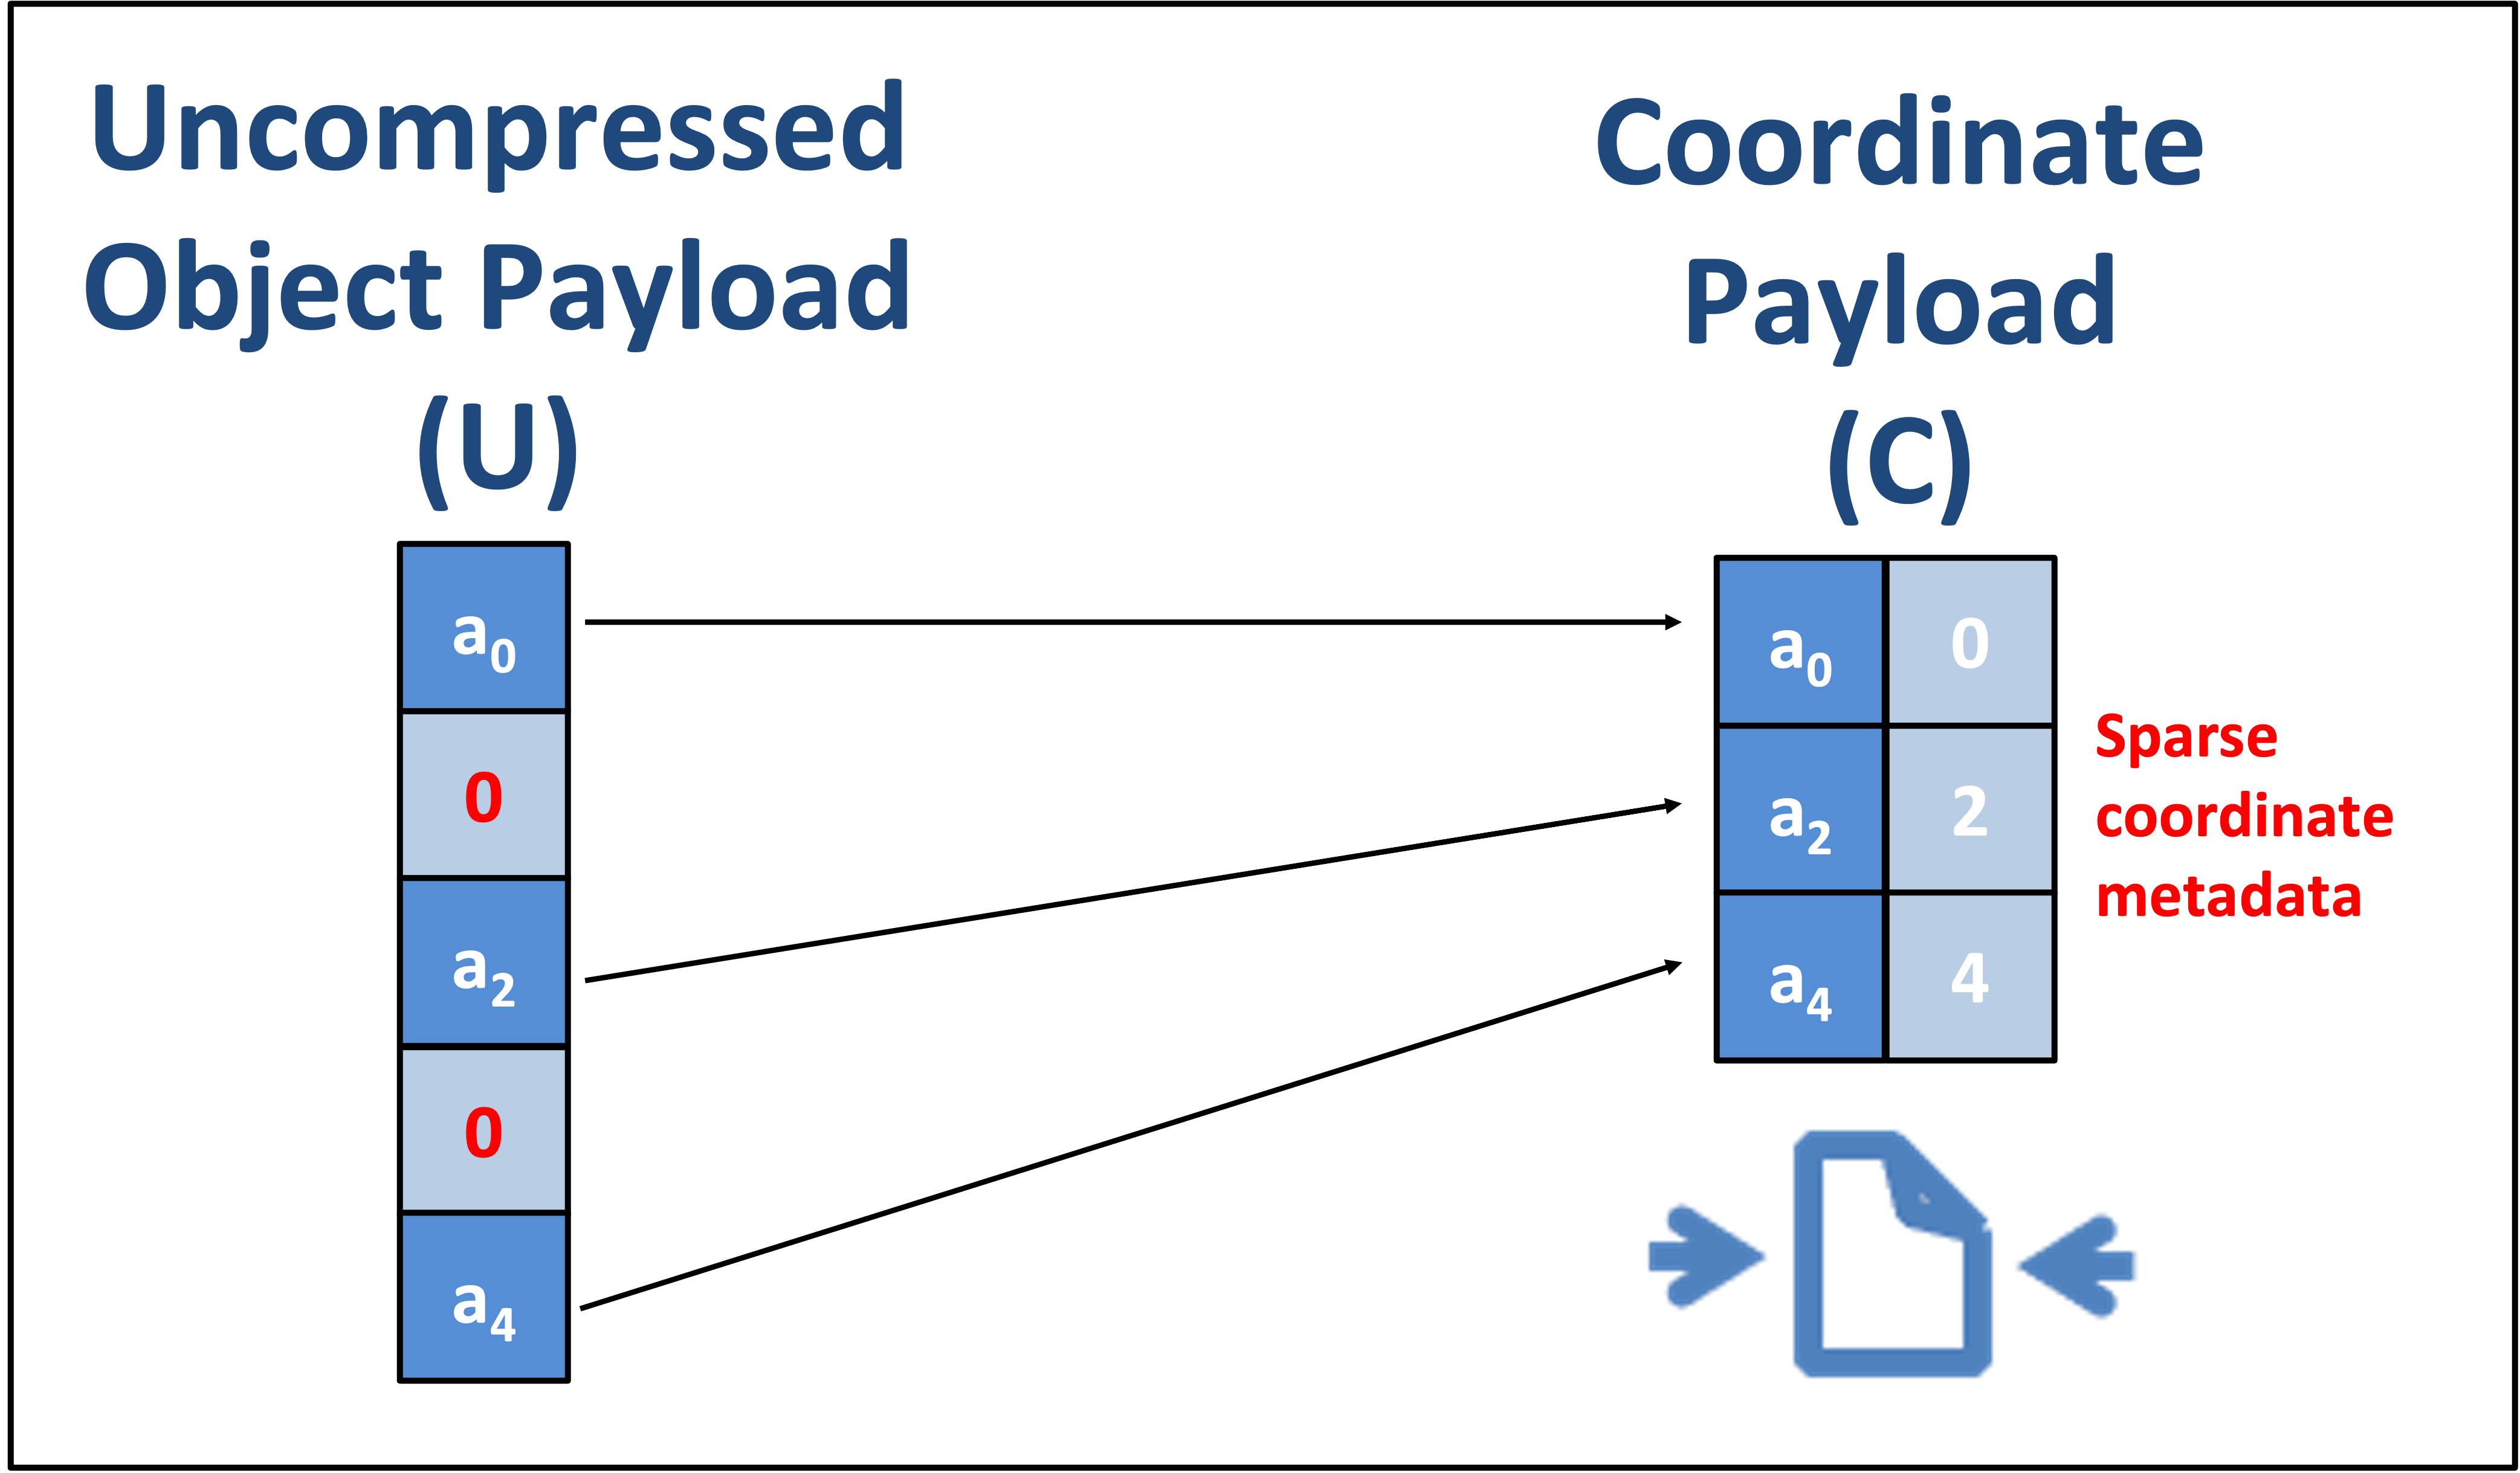
\includegraphics[width=8cm]{figures/saf_format_optimizations.PNG}
\caption{A visualization of a compressed representation format (coordinate-payload or CP) applied to a vector with some zero entries. The compressed representation is reduced to nonzero values and metadata which recovers the original data structure.}
\label{fig:saf_format_optimizations}
\end{figure}
%
% Content: format optimizations
%

%
% Figure: combined action/format optimizations
%
\begin{figure}[h]
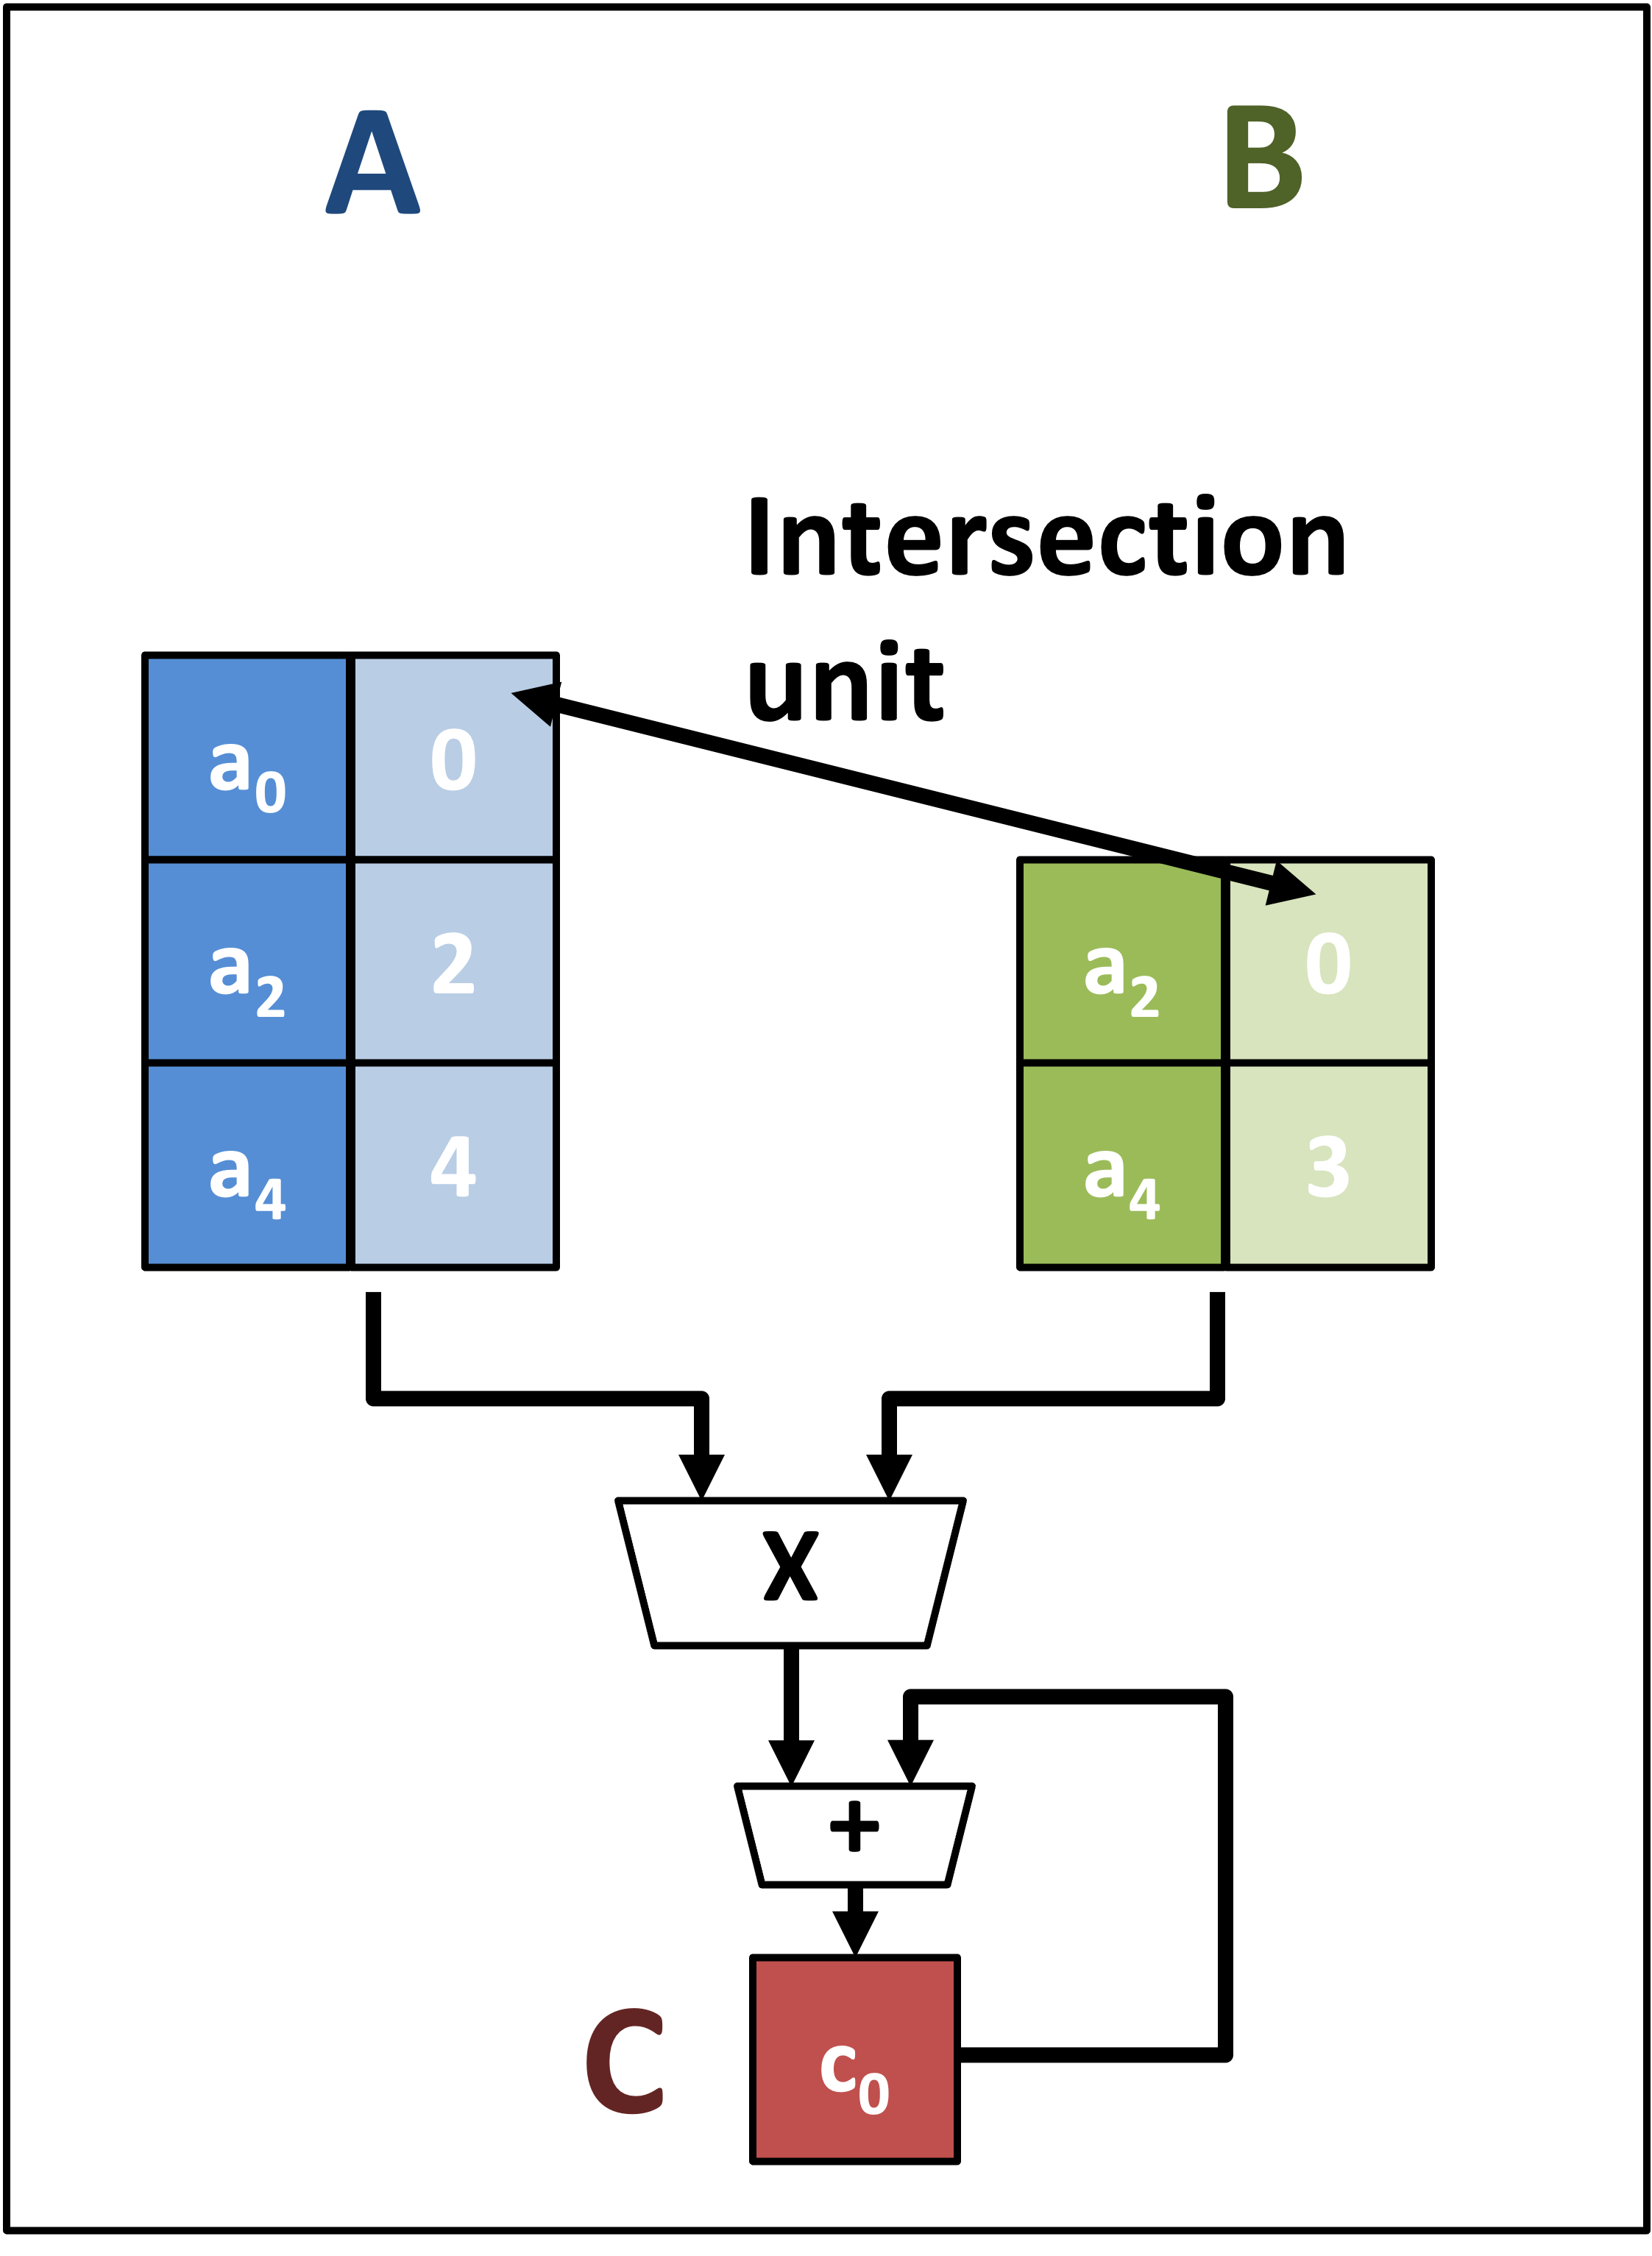
\includegraphics[width=4cm]{figures/saf_action_format_combo.PNG}
\caption{An example of dot-product optimized with both bidirectional zero-skipping and a compressed representation format. Conceptually corresponding nonzero values must be matched using a component which processes format metadata in order to implement skipping, which is called an \textit{intersection unit.} The cost of the skipping optimization is the energy, area and latency of the skipping microarchitecture, which comprises the intersection unit.}
\label{fig:saf_action_format_combo}
\centering
\end{figure}
%
% Figure: architecture example
%
\begin{figure}[h]
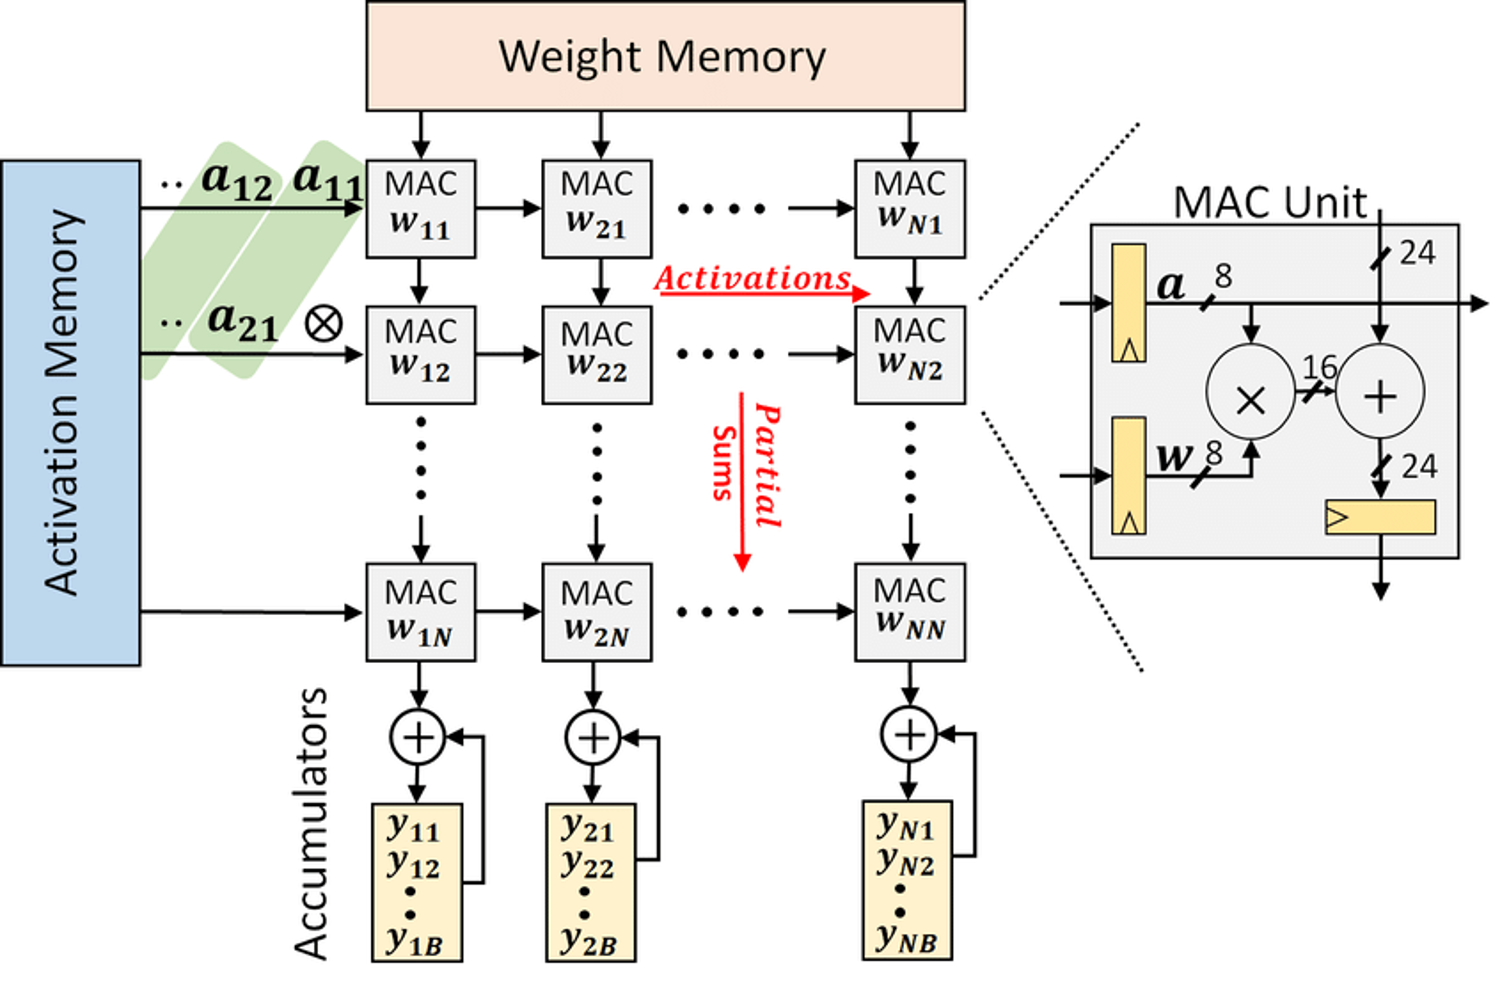
\includegraphics[width=8cm]{figures/arch_example.PNG}
\caption{A tensor accelerator \textit{architecture} (Thunderbolt architecture, figure from \cite{examplearch}.)}
\label{fig:saf_format_optimizations}
\end{figure}
%
% Figure: microarchitecture example
%
\begin{figure}[h]
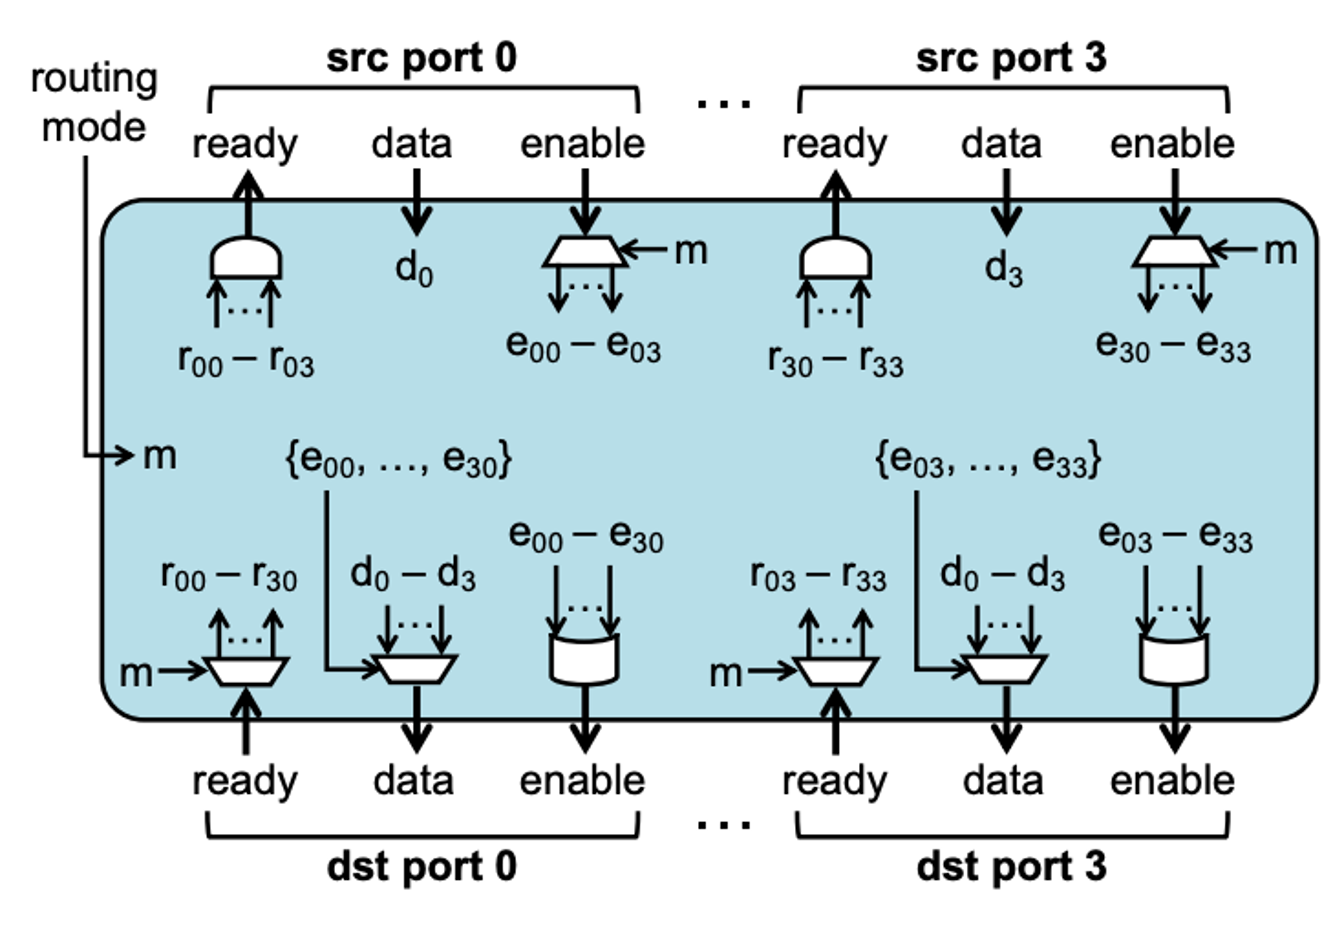
\includegraphics[width=8cm]{figures/uarch_example.PNG}
\caption{Tensor accelerator \textit{microarchitecture} (Eyeriss v2 NoC switch, figure from \cite{eyerissv2}.)}
\label{fig:saf_format_optimizations}
\end{figure}
%
% Figure: SAFs can be significant or not, it depends on the microarchitecture
%
\begin{figure*}[ht]
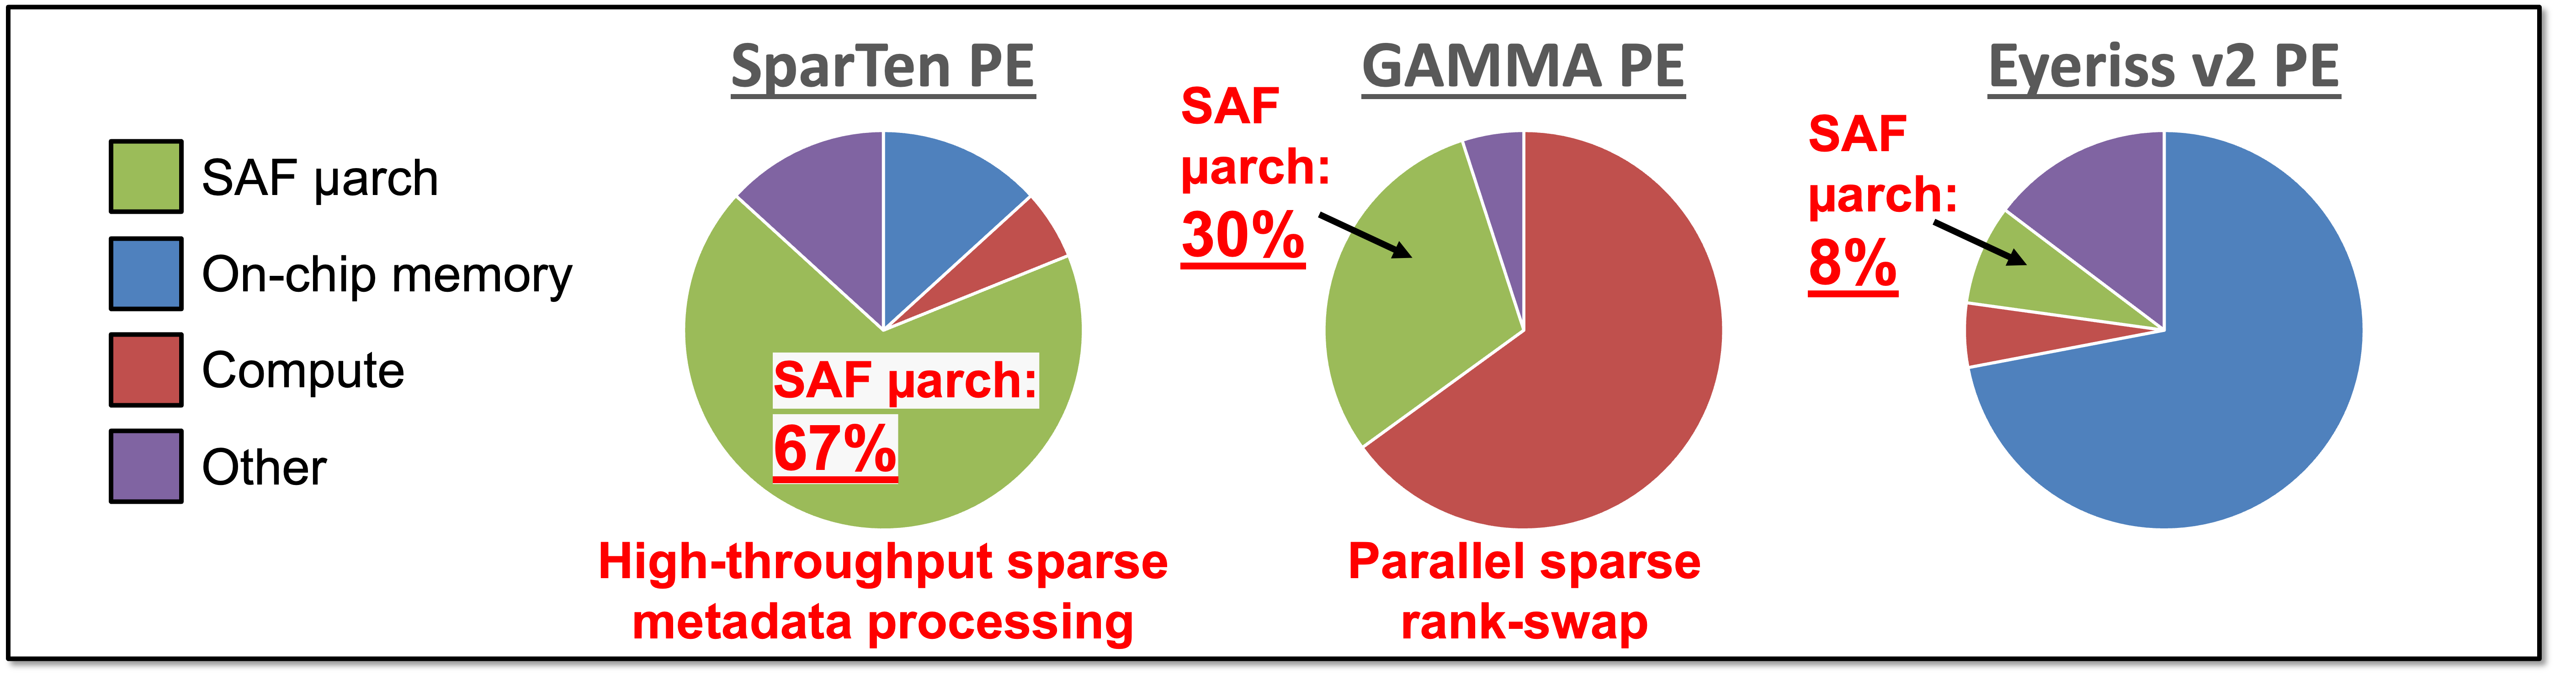
\includegraphics[width=\textwidth]{figures/saf_uarch_significance.PNG}
\caption{Breakdown of sparse tensor accelerator PE area based on published RTL simulations for a representative sample of designs. The total area of PE architectural components is a decent model of Eyeriss v2\cite{eyerissv2} PE area because Eyeriss v2's simple leader-follower zero-skipping microarchitecture has negligible area. SparTen\cite{sparten} employs a complex zero-skipping microarchitecture which must process high-throughput bitmask metadata. GAMMA's\cite{gamma} PE coordinates loop-nest re-ordering with tensor layout shuffling while the data is in-flight, using a high-radix merger component. These complex microarchitectures create discrepancies against architectural PE models.}
\label{fig:saf_uarch_significance}
\centering
\end{figure*}
%
% Figure: prior work
%
\begin{table*}[ht]
\begin{tabular}{c|c|}
\textbf{Accelerator} & \textbf{SAF microarchitecture proposals} \\ \hline \hline
Eyeriss &  MAC gating; in-flight RLE decompression \\ \hline
Eyeriss v2 & CSC zero-skipping \\ \hline
ExTensor & Hierarchical bidirectional zero-skipping \\ \hline
SCNN & Memory conflict handling (binning output coordinates) \\ \hline
SparTen & Bitmask zero-skipping, parallel compression, memory conflict handling \\ \hline
OuterSPACE & Software rank-swap \\ \hline
GAMMA & Leader-following intersection, hardware rank-swap \\ \hline
\end{tabular}
\caption{A non-exhaustive list of published tensor accelerators and their proposed SAF microarchitectures.}
\label{tab:design_specific_models}
\centering
\end{table*}

\section{SAF microarchitectures}

Prior research on sparse tensor acclerators proposes many different SAF microarchitectures, without employing a consistent set of abstractions and models in order to explore the design space or make comparisons. However, the breakdown of PE area for several accelerator designs in Figure~\ref{fig:saf_uarch_significance} shows that it is not always safe to assume SAF microarchitecture overhead is insignificant, and so it is important to choose SAFs and SAF microarchitecture designs systematically to minimize cost.

The Eyeriss v2\cite{eyerissv2} PE implements a leader-follower skipping SAF, devoting only 8\% of its PE area to the skipping microarchitecture. This is owing to a lightweight leader-follower skipping microarchitecture which operates on sparse weights and activations in Compressed-Sparse Column (CSC) format. 

In contrast, the SparTen\cite{sparten} accelerator PE uses most of its PE area for the bidirectional skipping microarchitecture which operates on Bitmask-format metadata. As will be shown later, this is attributable to the substantial load-handling capability which the skipping microarchitecture must have in order to maintain high arithmetic hardware utilization. 

As a final example, the GAMMA\cite{gamma} accelerator PE devotes 30\% of its PE area - a significant amount - in order to apply a rank swap\footnote{Here, rank swap is used to refer to transposition of the traversal-order of tensor ranks, as described in\cite{TODO}.}. The PE employs a row-wise product dataflow for loading CSR-format GEMM ($C_{M\times N} = A_{M\times K} \times B_{K\times N}$) operands from memory. A single $A_{M\times K}$ element and a row of $B_{K\times N}$ elements are loaded from on-chip memory into the PE; this reflects that the $N$ rank of B is traversed in the inner-most loop, while the contracted $K$ rank is traversed at an intermediate loop level. Row-wise product enables a cheap leader-follower skipping microarchitecture to be employed for loading $B_{K\times N}$ rows conditional on non-zero $A_{M\times K}$ elements. Upon receiving $A_{M\times K}$ and $B_{K\times N}$ values from memory, the GAMMA PE implements a rank-swap which moves the contracted dimension $K$ into the innermost loop. This enables inner-product accumulation into a single PE output register. The output memory footprint saved by the rank-swap is significant: a design such as MatRaptor\cite{matraptor} which implements row-wise product \textit{without} a rank-swap must store and incrementally accumulate $|K|$ rows of partial outputs, each of size $1 \times |N|$, requiring increased output memory footprint. Given the benefit of rank-swap, is there a tradeoff involved in using it? The use of CSR in GAMMA, means thank rank-swap requires a merge primitive (analogous to the merge operation in mergesort) in order to sort $B_{K\times N}$ operand data first by $K$ coordinate metadata, and then by $N$ coordinate metadata, effectively implementing a transpose. GAMMA employs a radix-64 merge unit\cite{gamma} in order to do this. Although the rank-swap itself is not a sparse optimization, nonetheless the need for this type of merge unit results from employing a rank-swapped dataflow \textit{in the context of employing CSR format for the $B_{K\times N}$ operand}. Thus it is justifiable to say that the merge unit is part of the format microarchitecture which implements the CSR format SAF. It is this format microarchitecture which accounts for 30\% of PE area in GAMMA.

Clearly, SAFs and SAF microarchitecture designs are complex and impactful design decisions, and it is desirable to know whether a particular combination of SAFs will lead to the substantial PE implementation overhead seen (for example) in SparTen and GAMMA. The rest of this work develops a conceptual framework for taxonomy and modeling of SAF microarchitectures. This conceptual framework can be represented in software and utilized for make SAF microarchitecture design decisions using analytical pre-RTL modeling tools.

%\subsection{Smartbuffer model and Format microarchitecture}
%\subsubsection{Dense smartbuffer}
%\subsubsection{Sparse smartbuffer}
%\subsubsection{Format interfaces}

\label{background:saf_uarch}
\chapter{SAF microarchitecture conceptual framework}
\label{chapter:conceptual_framework}

The \textit{Efficient Processing} framework presents a consistent set of abstractions for describing the impact of sparsity on microarchitecture. However, as discussed in Section~\ref{chapter:introduction} the goal of this work is to create a framework for defining SAF microarchitectures at a fine enough granularity to enable modeling and comparison between designs, while still keeping the framework general enough to describe a wide range of designs. A few challenges that come with applying the \textit{Efficient Processing} SAF microarchitecture taxonomy to this problem are

\begin{itemize}
    \item The components in the \textit{Efficient Processing} SAF microarchitecture taxonomy are black boxes without any associated models of area, actions, or energy. This makes evaluation or comparison of design choices more time-consuming because models must be designed from scratch.
    \item Among the \textit{Efficient Processing} primitives there is wide variation in complexity. Intersection units, position generators, and coordinate generators, for example, are relatively simple components. In contrast, the \textit{Efficient Processing} taxonomy also includes (for example) a number of different types of memories - in practice, memories may vary wildly in terms of i.e. what type of memory is employed (SRAM, DRAM, register file, etc.), how data orchestration is handled, what special features are supported (i.e. error correction), etc. Additionally, because the \textit{Efficient Processing} strives to show that sparse dataflows may be conceptually mapped to dataflow microarchitectures, microarchitecture designs created using the \textit{Efficient Processing} taxonomy are relatively complex.
    \item While it is helpful to have a consistent set of SAF microarchitecture abstractions that are decoupled from the fine details of manipulating sparse representation formats, this means that the co-design process will eventually run up against the difficulty of going from a high-level SAF microarchitecture topology built out of \textit{Efficient Processing} primitives, to a more fleshed-out design that is compatible with the sparse representation formats used to compress the operands.
    
\end{itemize}

Building on the \textit{Efficient Processing} SAF microarchitecture topology, this work applies three strategies to address the above challenges: 

\begin{itemize}
    \item Shrink the SAF microarchitecture design-space, by decoupling SAF microarchitecture from architecture and dataflow.
    \item Augment \textit{Efficient Processing} microarchitecture primitives with \textit{parameterization} and \textit{composition}. While the existing \textit{Efficient Processing} taxonomy is good for describing a \textit{format-agnostic} SAF microarchitecture, parameterization and composition will enable a systematic process for deriving an elaborated SAF microarchitecture that is \textit{co-designed} for dataflow and sparse representation format.
    \item Associate each SAF microarchitecture primitive with an analytical cost model, enabling evaluation and comparison between designs.
\end{itemize}

% Extending Efficient Processing framework

% Decoupling SAF microarchitecture from dataflow
% - Narrower definition of SAF microarchitecture
% - => Coupled access
% - Managing SAF microarchitecture/representation format co-design through parameterization
% - => Parameterization for capturing additional design flexibility
% - Decoupling from dataflow through boundary conditions
% - => High-level intro
% - Additional notes on prior work
% - => Skipping topologies & always having pgen
% - => Pgen reference
% - => Fill optimizers
% - Overview of proposed conceptual framework
% - => Buffer model & format interfaces
% - => Workload modeling
% - => SAF uarch component - fmt- and dataflow-indep
% - => Taxo of parameterized primitives & models
% - => 

Starting from these principles, this section shows builds up a conceptual framework based on these three strategies, making sure to integrate insights from prior work on sparse tensor accelerators.

\section{Decouple SAF microarchitecture from architecture and dataflow}
\label{sec:what_is_a_saf_microarchitecture}

\textit{Efficient Processing} attempts to design a rough correspondence between sparse dataflow loop nests, and microarchitectural topologies\cite{szebook}. However, in this work, the correspondence between sparse loop nests and microarchitectural topologies is eschewed in favor of focusing on \textit{the correspondence between the Sparseloop\cite{sparseloop} SAF declaration, and the underlying SAF microarchitecture.} Note that a Sparseloop SAF carries no information about dataflow. This change of focus permits us to sharply delineate what qualifies as a SAF microarchitecture component:

\begin{itemize}
    \item If a microarchitectural component or circuit is introduced by an author with the explicit goal of allowing a design to exploit sparsity in some way, that is a SAF microarchitecture.
    \item A microarchitectural component which, if removed or replaced with a naive implementation, would render the accelerator unable to cope with traversing, co-iterating, or otherwise working with sparse representation formats, is a SAF microarchitecture.
\end{itemize}

What is \textit{not} a SAF microarchitecture:

\begin{itemize}
    \item Any architectural component - buffer, compute, etc. - is not SAF microarchitecture.
    \item Any microarchitecture which is not unique to sparse tensor accelerators, is not SAF microarchitecture (i.e. the microarchitectural details of switches within a NoC, unless there are \textit{specific optimizations for network routing in the presence of sparsity}, do not comprise SAF microarchitecture)
    \item In this work \textit{dataflow} is conceived of as something that architecture \textit{does}; since architecture is excluded from SAF microarchitecture, any logic which implements dataflow is by default not SAF microarchitecture. This excludes, for example, most address generators or sequence generators, such as the \textit{Efficient Processing} position generator and coordinate generator components. However, microarchitectures which implement dataflow \textit{in a specific fashion to account for sparsity}, would count as SAF microarchitecture.
\end{itemize}

\subsection{Sequence generators and decoupled orchestration}

\textit{Efficient Processing}\cite{szebook} primarily focuses on describing EDDO\cite{buffet} accelerators; thus, the \textit{position generator} and \textit{coordinate generator} components in the \textit{Efficient Processing} taxonomy serve to implement EDDO dataflows, by generating pre-determined sequences of position or coordinate values, respectively.

Thus, we will refer to these components as \textit{decoupled} position generators and \textit{decoupled} coordinate generators, respectively.

Going forward, this work assumes that all architectural memories are \textit{smartbuffers}\cite{smartbuffer}, memories with integrated logic for decoupled traversal of stored tensors.

\subsection{Reclassifying the \textit{Efficient Processing} taxonomy}

Table~\ref{tab:reclassify_saf_microarchitecture} reclassifies the \textit{Efficient Processing} taxonomy in Figure~\ref{fig:efficient_processing_taxo} based on the aforementioned more-stringent criteria for what qualifies as SAF microarchitecture.

\begin{table}
\centering
\caption{Reclassification of \textit{Efficient Processing}\cite{szebook} primitives}
\label{tab:reclassify_saf_microarchitecture}
\begin{tabular}{||p{0.3\textwidth}|l|l||}\hline
\textbf{SAF $\mu$arch} & \textbf{Non-SAF $\mu$arch} & \textbf{Architecture}  \\\hline
Intersection & \textit{Decoupled} pgen & Uncompressed data buffer \\\hline
\textit{Coupled} cgen & \textit{Decoupled} cgen & Updating uncompressed data buffer \\\hline
\textit{Coupled} pgen & Coordinate calculator & Compressed data buffer \\\hline
Support for coordinate calculations against sparse formats &  & Latch \\\hline
 &  & MAC \\\hline
\end{tabular}
\end{table}



\section{Decoupling SAF microarchitecture from dataflow via \textit{workload boundary conditions}}

In this work, the key to decoupling dataflow from SAF microarchitecture modeling is to encapsulate memory internals inside an abstract smartbuffer with a format-agnostic interface (Figure~\ref{fig:sparse_sbuff_overview}.) 

\begin{figure}[ht]
    \centering
    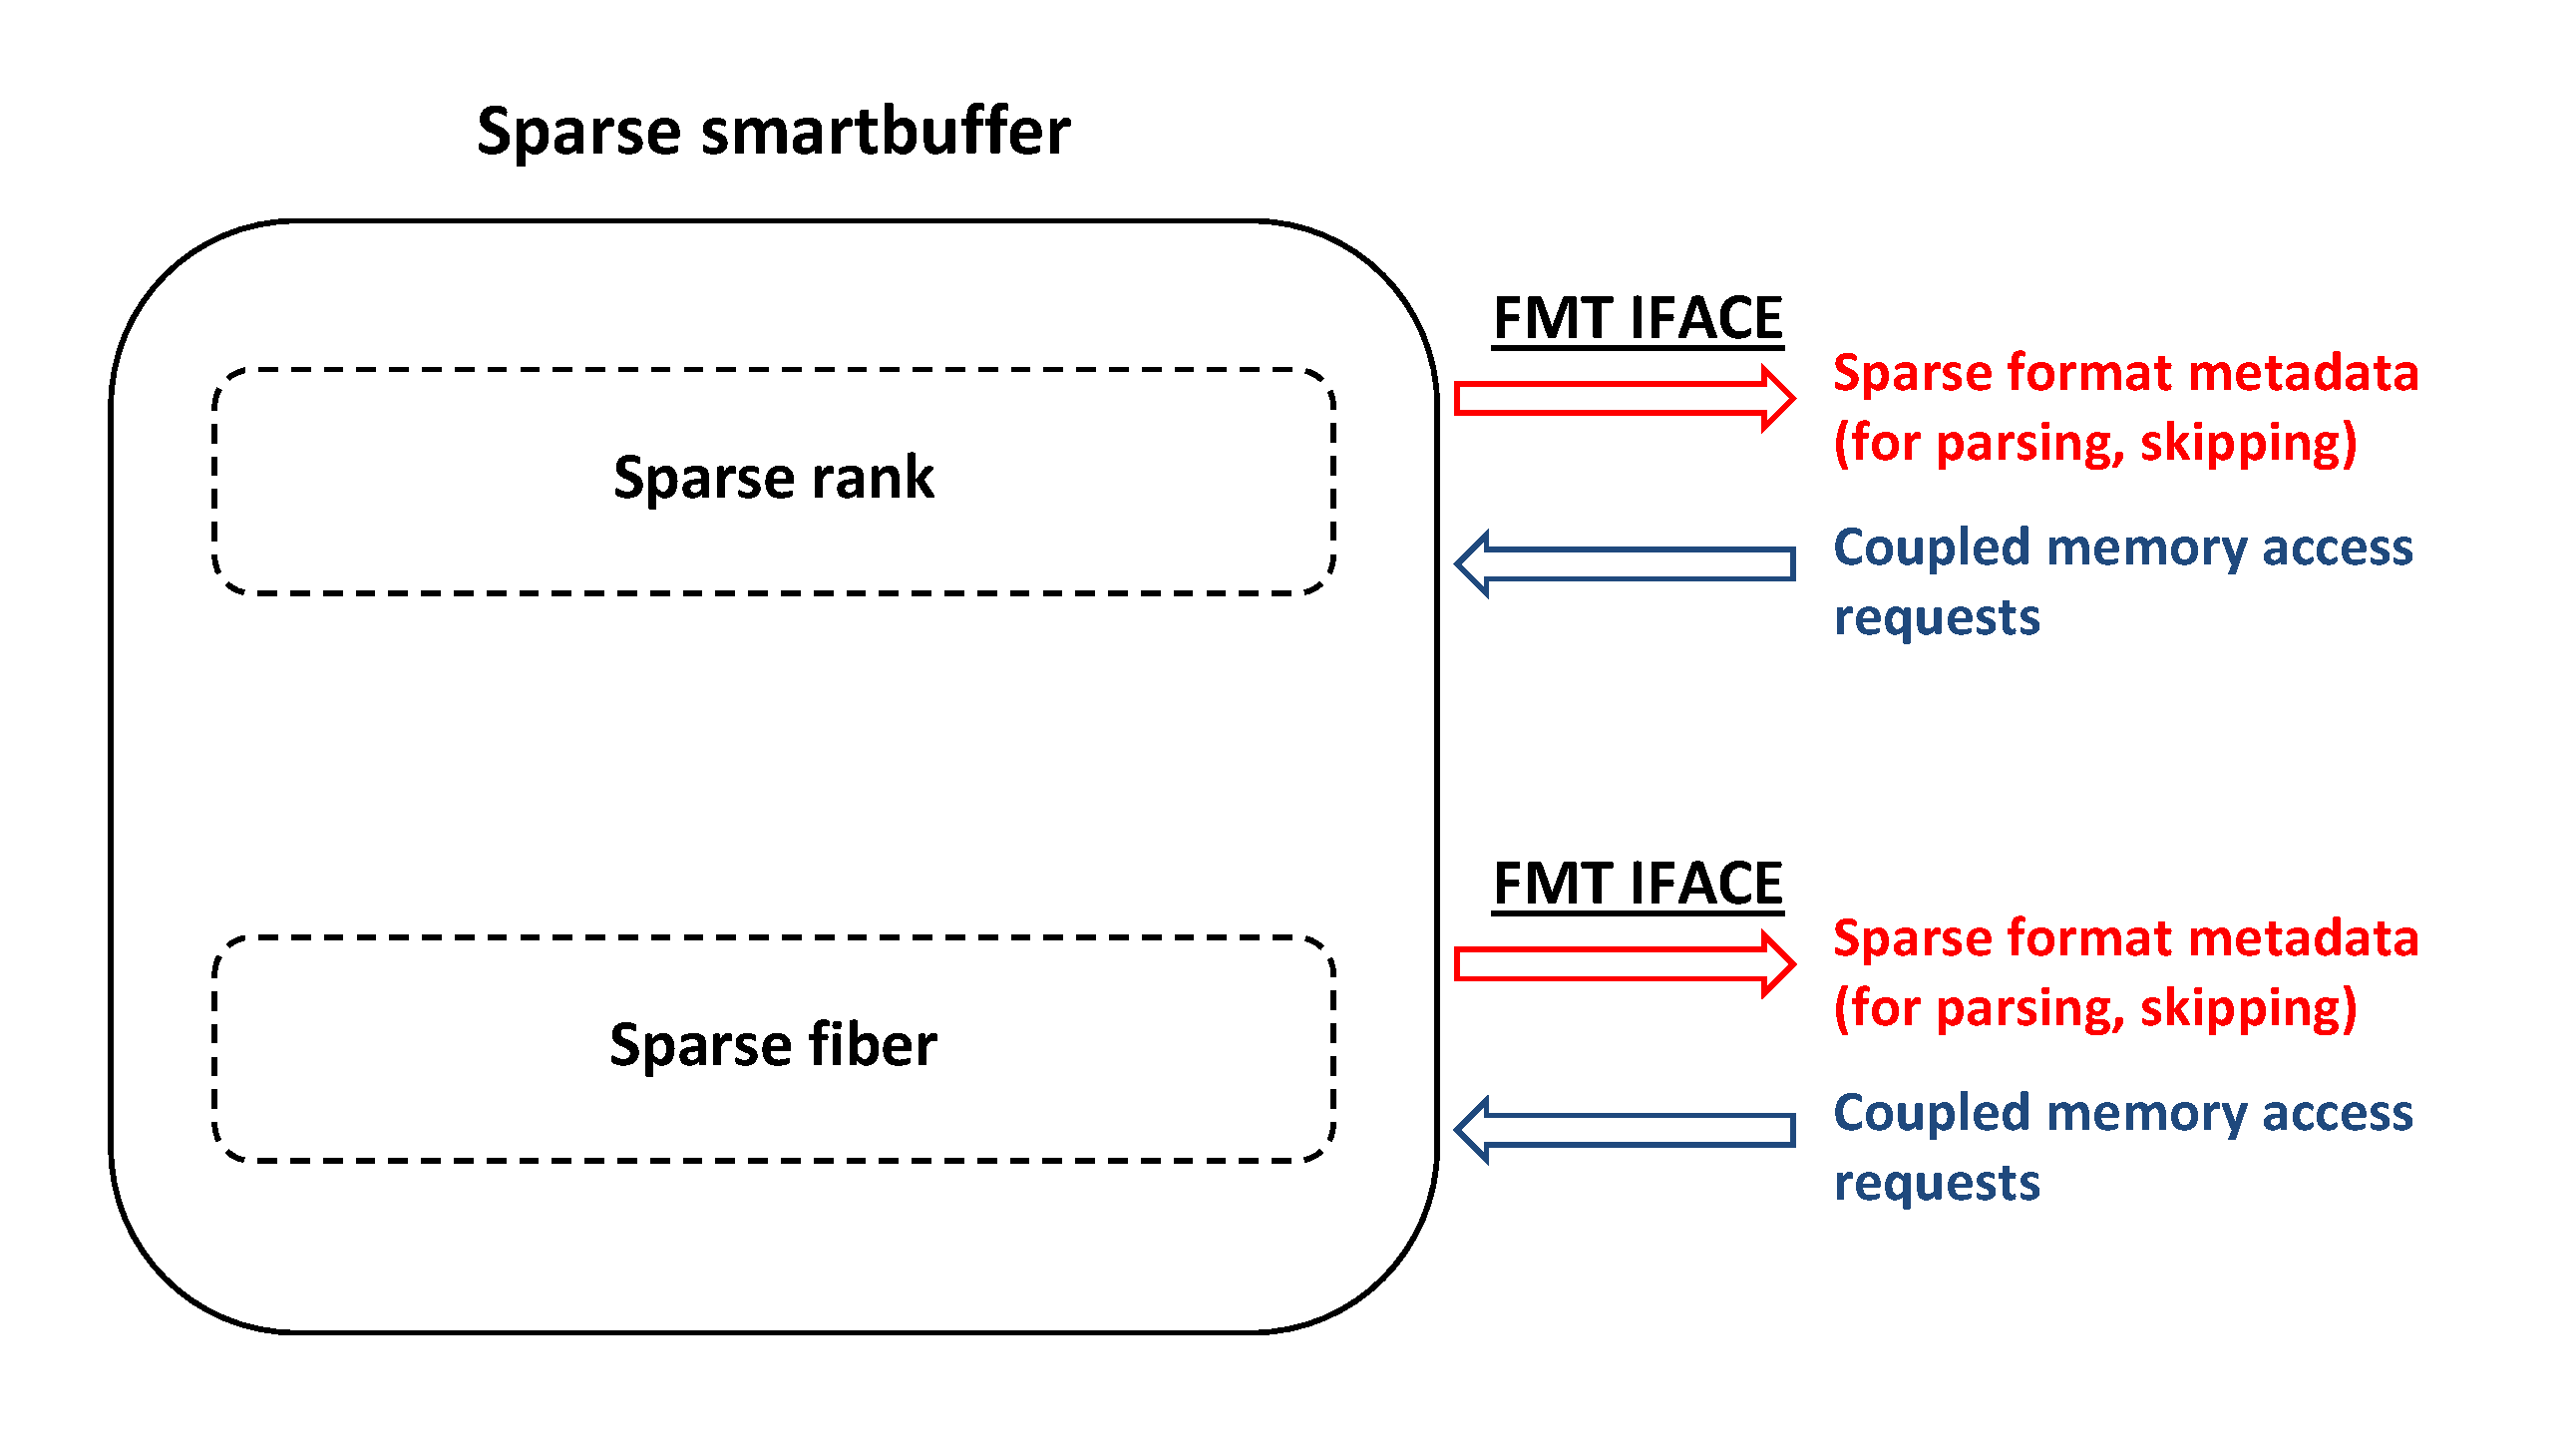
\includegraphics[width=0.95\textwidth]{figures/sparse_sbuff_overview.pdf}
    \caption{In this work, the details of memory implementation are encapsulated inside an abstract ``sparse smartbuffer'' with an identical IO bundle interface to each sparse rank. SAF microarchitecture can issue requests to a format interface in order to read a sparse rank's format metadata or trigger a payload read from a specified positional offset.}
    \label{fig:sparse_sbuff_overview}
\end{figure}

Each fibertree rank resident in the buffer, is hidden behind a format-agnostic IO bundle, called the ``format interface'' (fmt iface.) The format interface supports three operations:

\begin{itemize}
    \item \textbf{Get sparse fiber metadata:} Read a stream of sparse format metadata associated with one fiber in a given rank.
    \item \textbf{Request payload read at specified positional offset:} Coupled data orchestration is supported via input wires in the format interface IO bundle, which allow SAF microarchitecture to override the smartbuffer's internal decoupled data orchestration. Where EDDO data orchestration is desired, the format interface IO bundle inputs can simply be left unconnected.
    \item \textbf{Signal end-of-fiber:} Although \textit{Efficient Processing}\cite{szebook} focuses on EDDO data orchestration, some sparse dataflow microarchitectures proposed in the book have a limited amount of coupled data orchestration, in the form of one-bit flags which synchronously reset the otherwise decoupled sequence generators when the end of a fiber is reached. In this work, the format interface IO bundle includes a flag for signaling that the end of a fiber has been reached. The assumption here is that recognizing the end of a fiber may require specialized format metadata parsing within the SAF microarchitecture, and thus the format interface requires a flag input for the SAF microarchitecture to signal end-of-fiber to the rank's decoupled traversal logic.
\end{itemize}

Note the particular usage of ``encapsulation'' in this work: for the purposes of describing and modeling SAF microarchitecture, the internals of each sparse smartbuffer are not simply hidden behind the format interface, but rather are not implemented or modeled at all. The goal instead is to (1) define a consistent abstraction for the interface between architectural smartbuffers and SAF microarchitecture, and (2) define a set of \textit{workload boundary conditions} which are \textit{consistent} with sparse smartbuffer functionality under worst-case dataflow conditions. Here, \textit{workload} refers to any appropriate measure of the processing effort that is required of a SAF microarchitecture connected to the IO. Once the worst-case workload requirements are estimated for all format interfaces, then the SAF microarchitecture may be designed to satisfy the workload requirements, without regard to the overall dataflow. 

Figure~\ref{fig:sparse_sbuff_wkld_overview} provides a high-level overview of how workload boundary conditions are bound to format interfaces on a sparse smartbuffer. Note that all workload measures have a \textit{direction} which matches the IO they apply to. In Figure~\ref{fig:sparse_sbuff_wkld_overview}, the $w_{md}$ workloads (red) are bound to format interface output wires; $w_{md}$ is a measure of the processing effort imposed on the \textit{input port} of any SAF microarchitecture connected to the format interface output wires. The $w_{pos}$ workloads (blue) are bound to format interface input wires; $w_{pos}$ is a measure of the processing effort imposed on the \textit{output port} of any SAF microarchitecture connected to the format interface input wires.

\begin{figure}[ht]
    \centering
    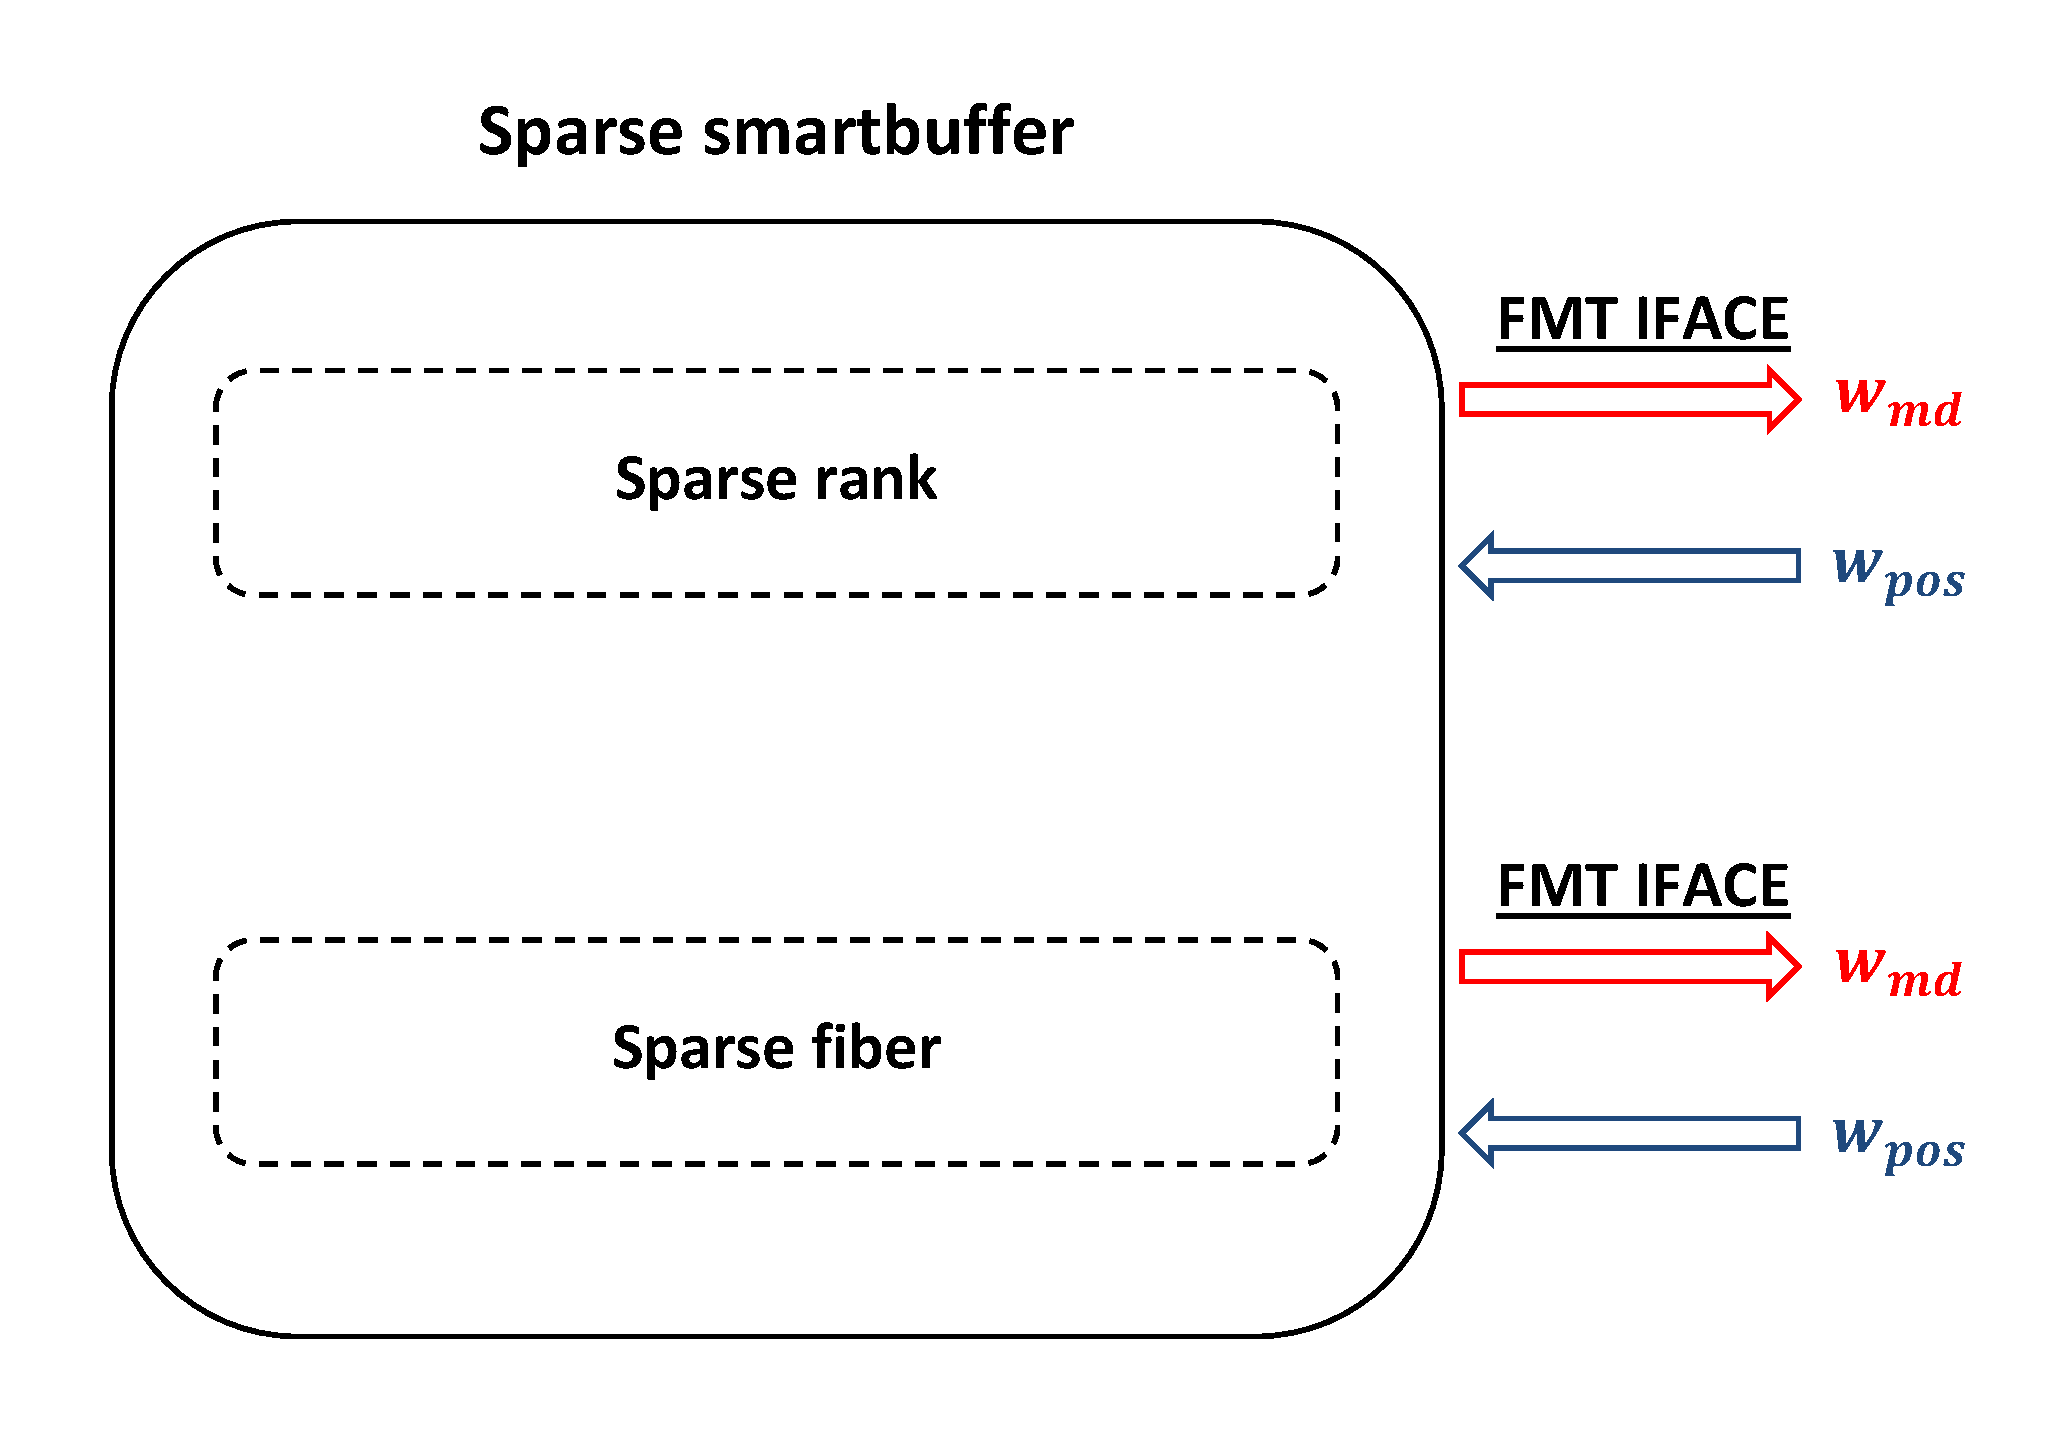
\includegraphics[width=0.95\textwidth]{figures/sparse_sbuf_wkld_overview.pdf}
    \caption{Sparse dataflow is abstracted behind \textit{workload boundary conditions}}.
    \label{fig:sparse_sbuff_wkld_overview}
\end{figure}

% Architecture, non-SAF microarchitecture, SAF microarchitecture



\subsection{Sparse smartbuffer model}

Although this work is not focused on modeling sparse smartbuffers, nonetheless it is helpful to develop a ``reference design'' for what a sparse smartbuffer implementation might look like. There are two reasons for this

\begin{itemize}
    \item \textbf{Define the format interface IO bundle.} Creating a sparse smartbuffer reference design helps us to be very concrete about what input and output wires a format interface must have, in order to support the most common workloads that operate on sparse fibers.
    \item \textbf{Workload modeling.} A mental model of sparse smartbuffer internals will be helpful later on when we bind workload measures to format interfaces.
\end{itemize}

This section will build up a reference design for a sparse smartbuffer in steps: (1) describe a single-fiber sparse smartbuffer for explicit-coordinate representation formats, (2) describe a single-fiber sparse smartbuffer for general explicit/implicit coordinate representation formats, and finally (3) describe a pipelined sparse smartbuffer capable of traversing a fibertree with support for general explicit/implicit coordinate representation formats.

\subsubsection{Composition}
\label{sec:composition}

A sparse smartbuffer can utilize some components which are familiar from dense smartbuffers\cite{buffet}\cite{sparseloop}, however, the sparse smartbuffer must have additional logic for operating on sparse fibers in order to correctly traverse a sparse fiber. Recall from Section~\ref{sec:what_is_a_saf_microarchitecture} that a SAF microarchitecture refers to that subset of an accelerator's microarchitecture, which either (1) was designed for processing sparse representation formats, or (2) is critical for the accelerator to correctly process sparse representation formats. This work is focused on describing and modeling SAF microarchitectures; since we ultimately are not striving to model smartbuffer internals, it is desirable to completely decouple the smartbuffer's sparse format processing logic into a separate component.

\begin{figure}[ht]
    \centering
    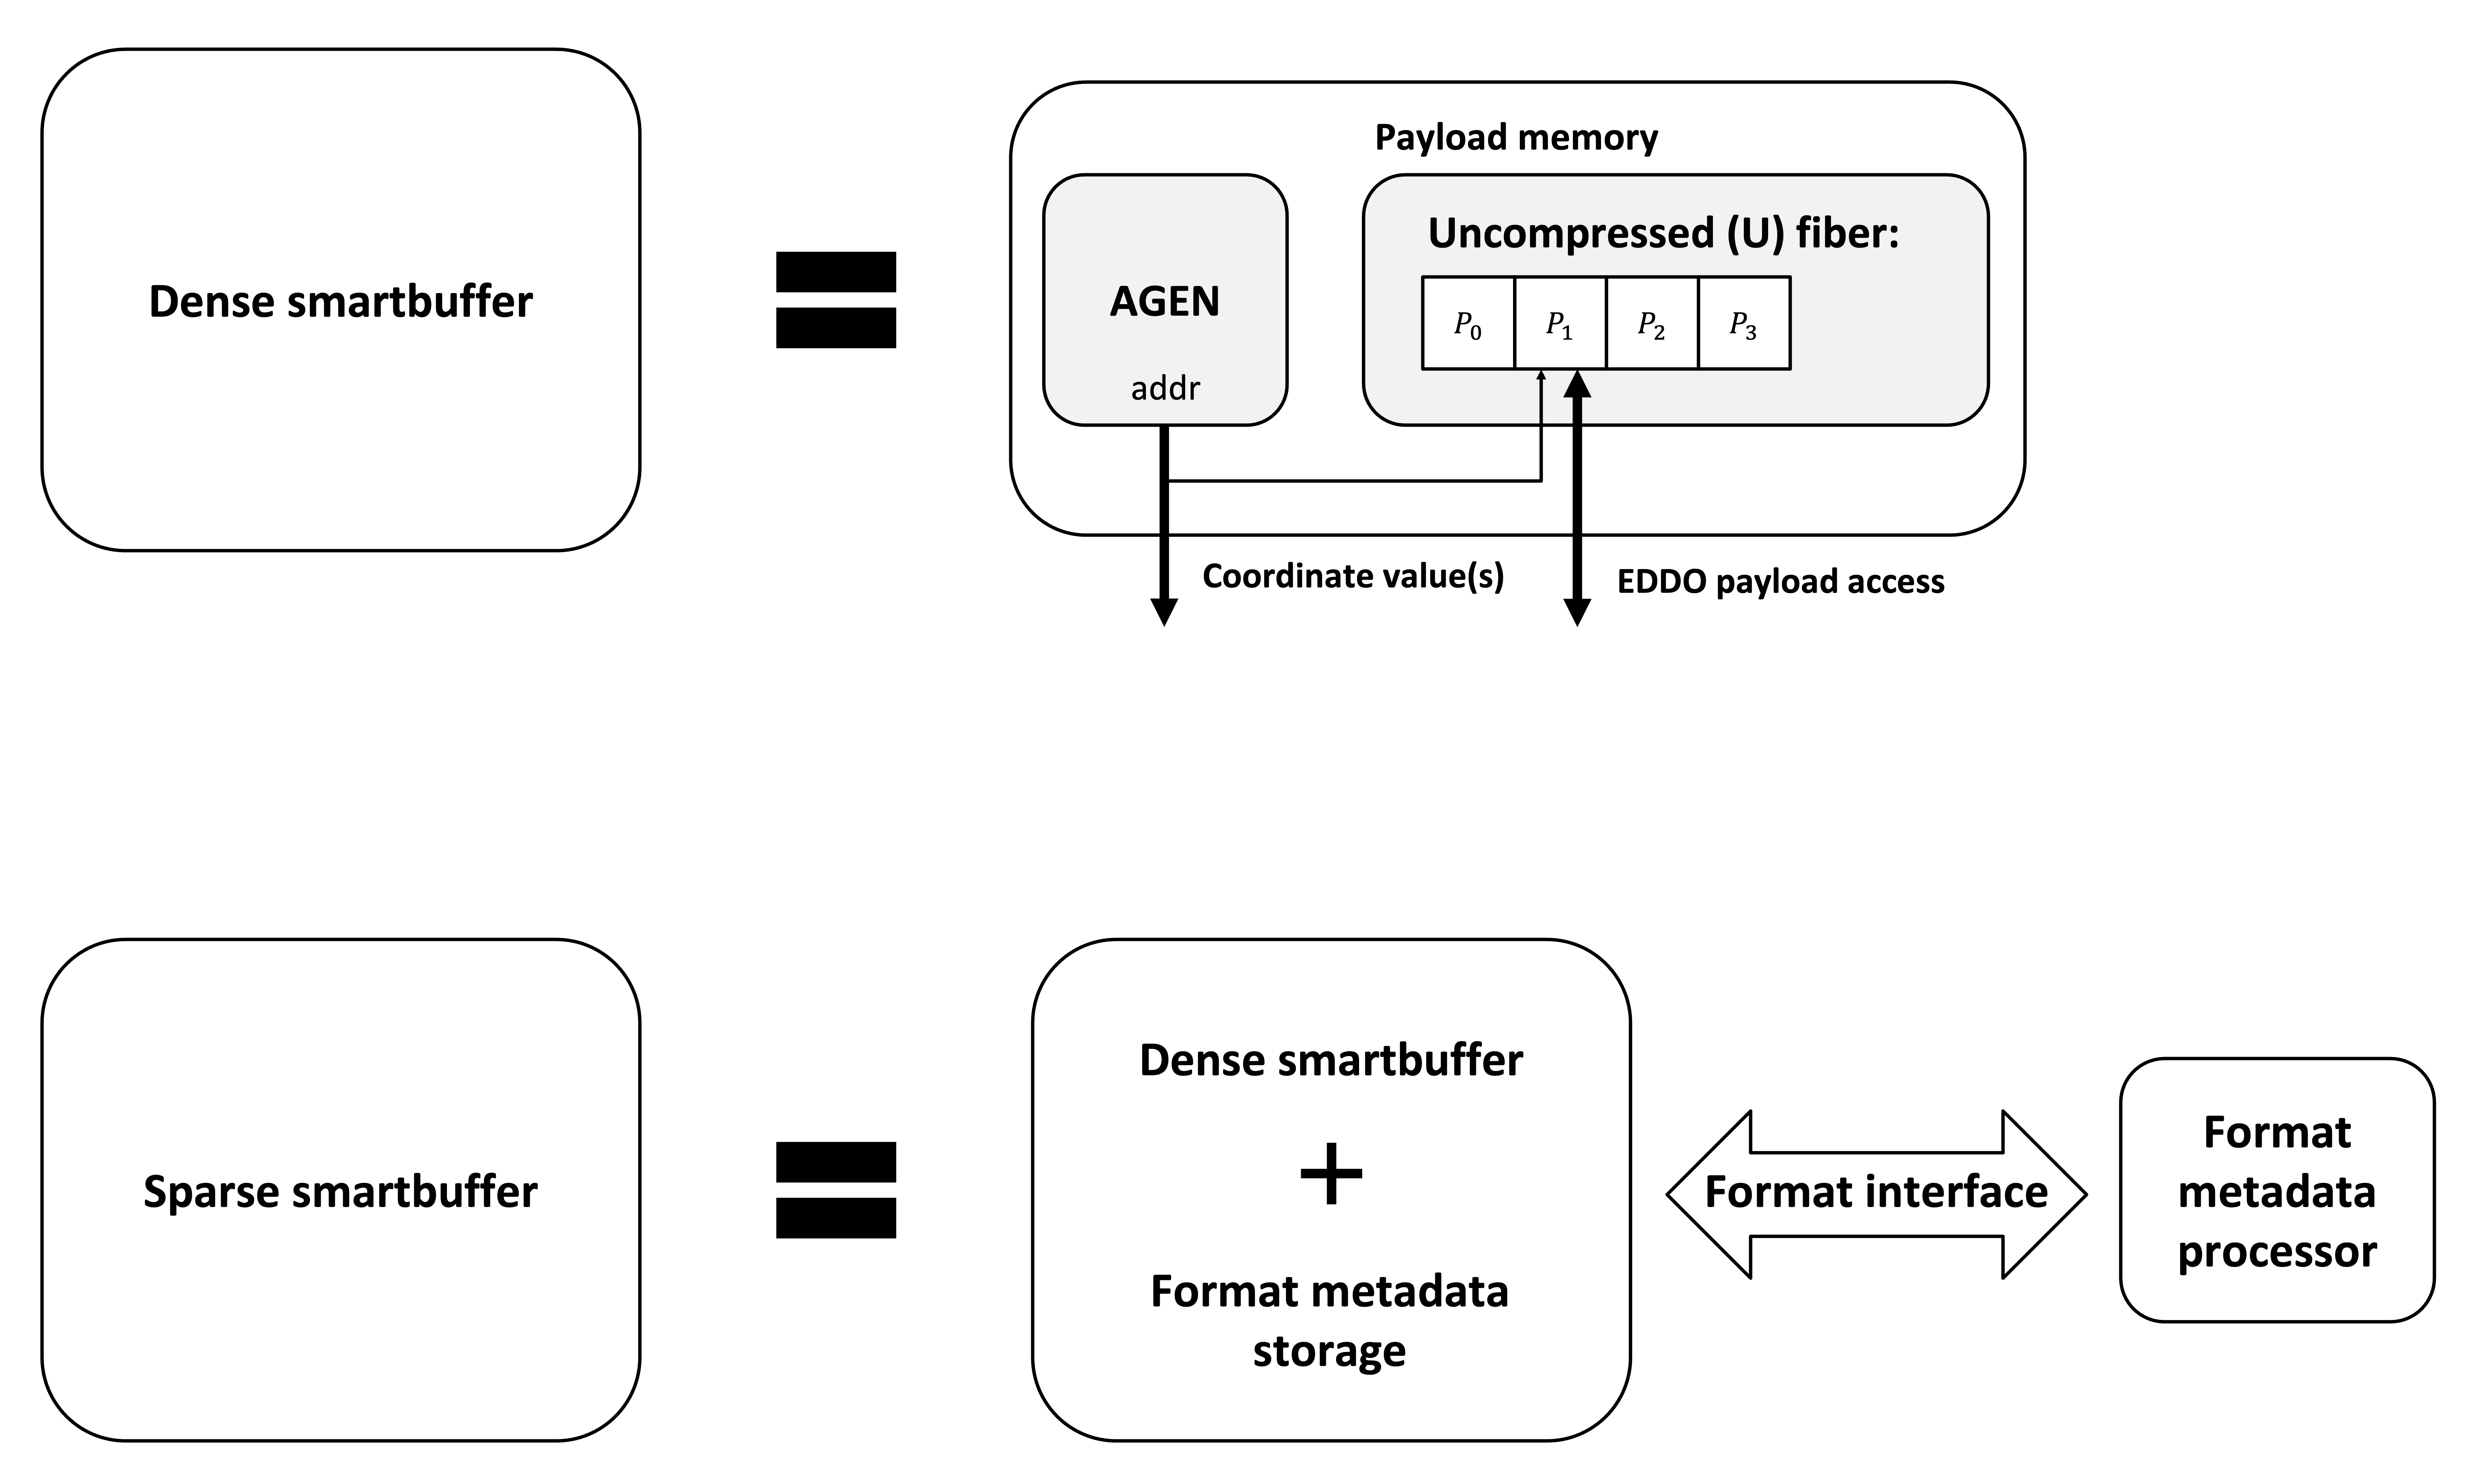
\includegraphics[width=0.95\textwidth]{figures/dense_smartbuffer_composition.png}
    \caption{This work models a \textit{sparse smartbuffer} as the composition of a dense smartbuffer with additional hardware that handles the compressed sparse tensor format, connected by an I/O bundle (``format interface''.) The format interface moves sparse format metadata from the dense smartbuffer metadata storage to the format metadata processor, and moves control signals in the other direction.}
    \label{fig:dense_smartbuffer_composition}
\end{figure}

Figure~\ref{fig:dense_smartbuffer_composition} (\textit{bottom}) shows how the sparse smartbuffer is modeled as a dense smartbuffer (\textit{top}) composed with (1) additional storage for sparse format metadata, and (2) a SAF microarchitecture that can process sparse format metadata. 

The dense smartbuffer in Figure~\ref{fig:dense_smartbuffer_composition} (\textit{top}) only holds one fiber; the AGEN unit implements decoupled fiber traversal by generating a stream of coordinate values which lookup into the uncompressed fiber (position and coordinate are synonymous for an uncompressed fiber.)

When the smartbuffer is storing a compressed sparse fiber, it becomes reliant on the SAF microarchitecture to receive sparse format metadata that is output through the format interface, and to send back control signals which ensure correct traversal.

\subsubsection{Single-rank, explicit-coordinate-format sparse smartbuffer model}
\label{sec:single_explicit_fiber}

Building on Section~\ref{sec:composition}, we can flesh out how the sparse smartbuffer internals and the format interface might be designed if the sparse fiber uses an explicit coordinate\cite{szebook} format such as coordinate-payload (C)\cite{szebook}.

\begin{figure}[ht]
    \centering
    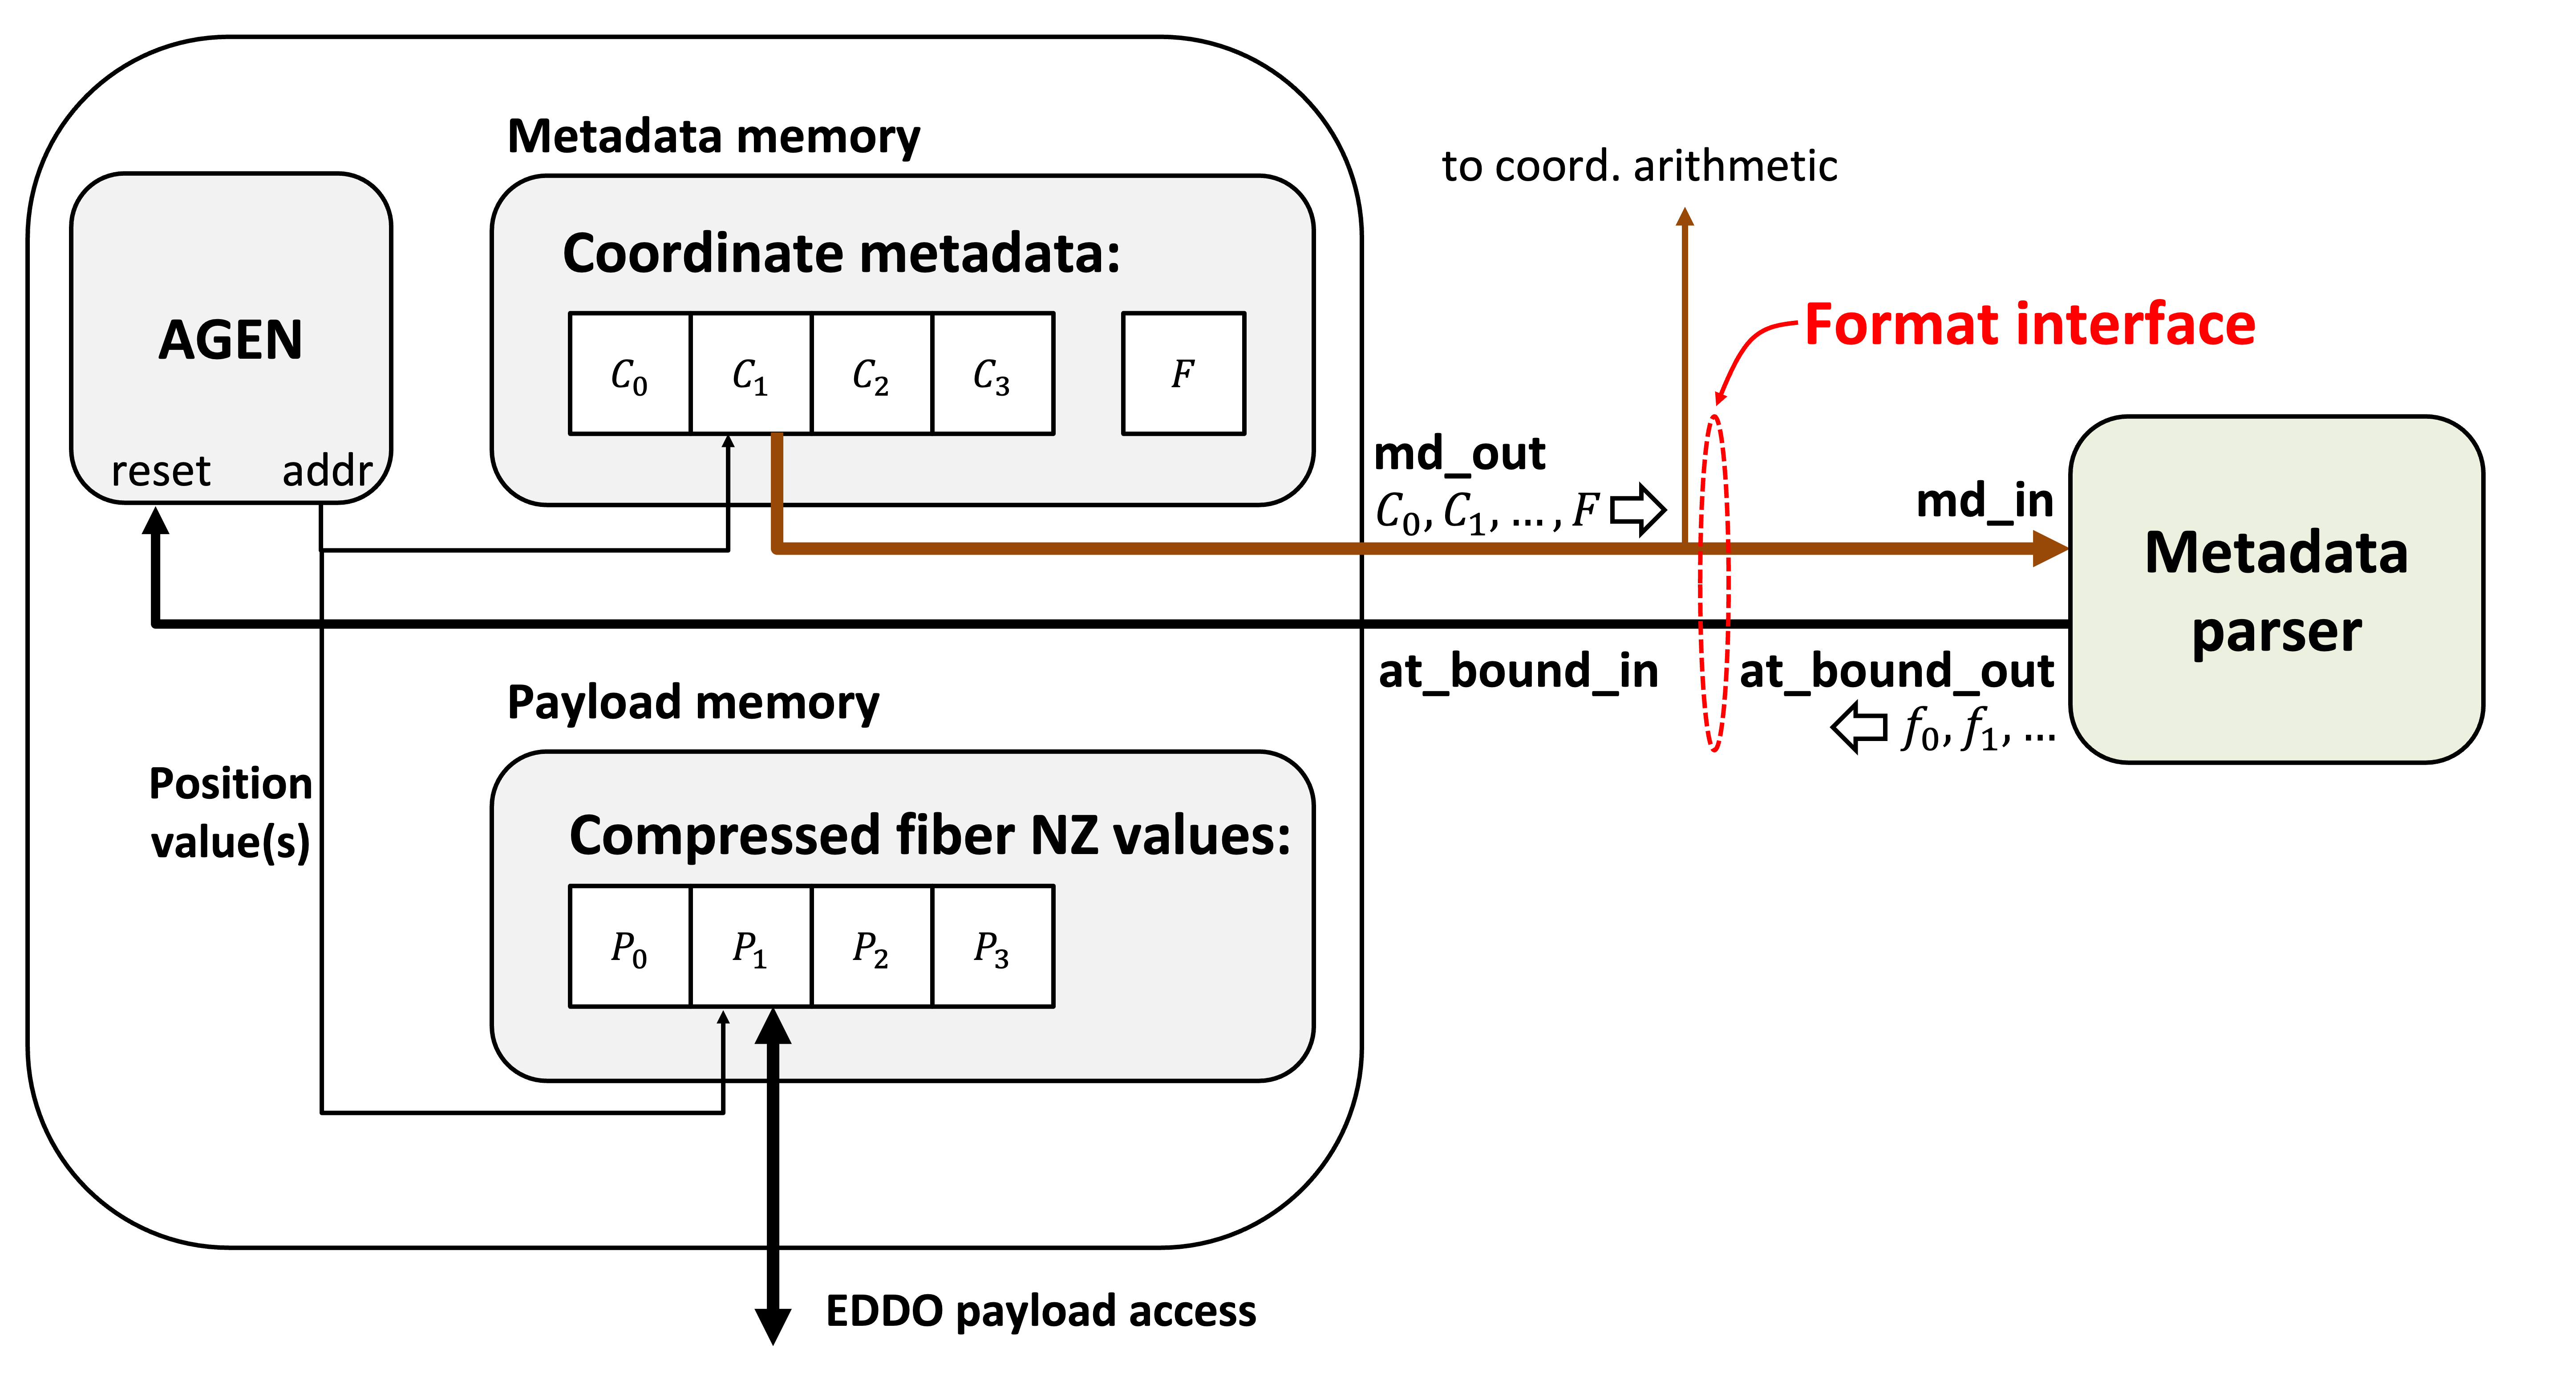
\includegraphics[width=0.95\textwidth]{figures/single_rank_explicit_coordinate_smartbuffer_model.png}
    \caption{Sparse smartbuffer model for a single rank, supporting explicit coordinate sparse tensor formats. ${C_i}$ are explicit coordinate metadata values. $F$ is a stand-in for any metadata regarding fiber characteristics, i.e. number-of-non-zeros. ${f_i}$ are flag values - metadata parser parses metadata arriving at md\_in and sets at\_bound\_out when fiber traversal is complete.}
    \label{fig:single_rank_explicit_coordinate_smartbuffer_model}
\end{figure}

In the coordinate-payload format, each non-zero/non-empty payload is paired with a coordinate metadata value. Figure~\ref{fig:single_rank_explicit_coordinate_smartbuffer_model} shows how the address generator implements traversal by looking up corresponding elements in the \textit{coordinate metadata} and \textit{compressed fiber non-zero (NZ) values} arrays. 

The only role for the metadata parser is to detect when the entirety of the fiber has been processed, and send a reset signal back over the format interface in order reset the traversal. Thus, the format interface consists simply of

\begin{itemize}
    \item \textbf{md\_out (output):} Output a stream of explicit coordinates to the metadata parser.
    \item \textbf{at\_bound\_in (input):} Receive the reset signal from the metadata parser upon completing fiber traversal.
\end{itemize}

\subsubsection{Single-rank, general-format sparse smartbuffer model}

It becomes apparent that the format interface and reference design in Section~\ref{sec:single_explicit_fiber}, while sufficient for an explicit-coordinate sparse format, are insufficient for an implicit-coordinate sparse format such as bitmask (B)\cite{szebook}.

\begin{figure}[ht]
    \centering
    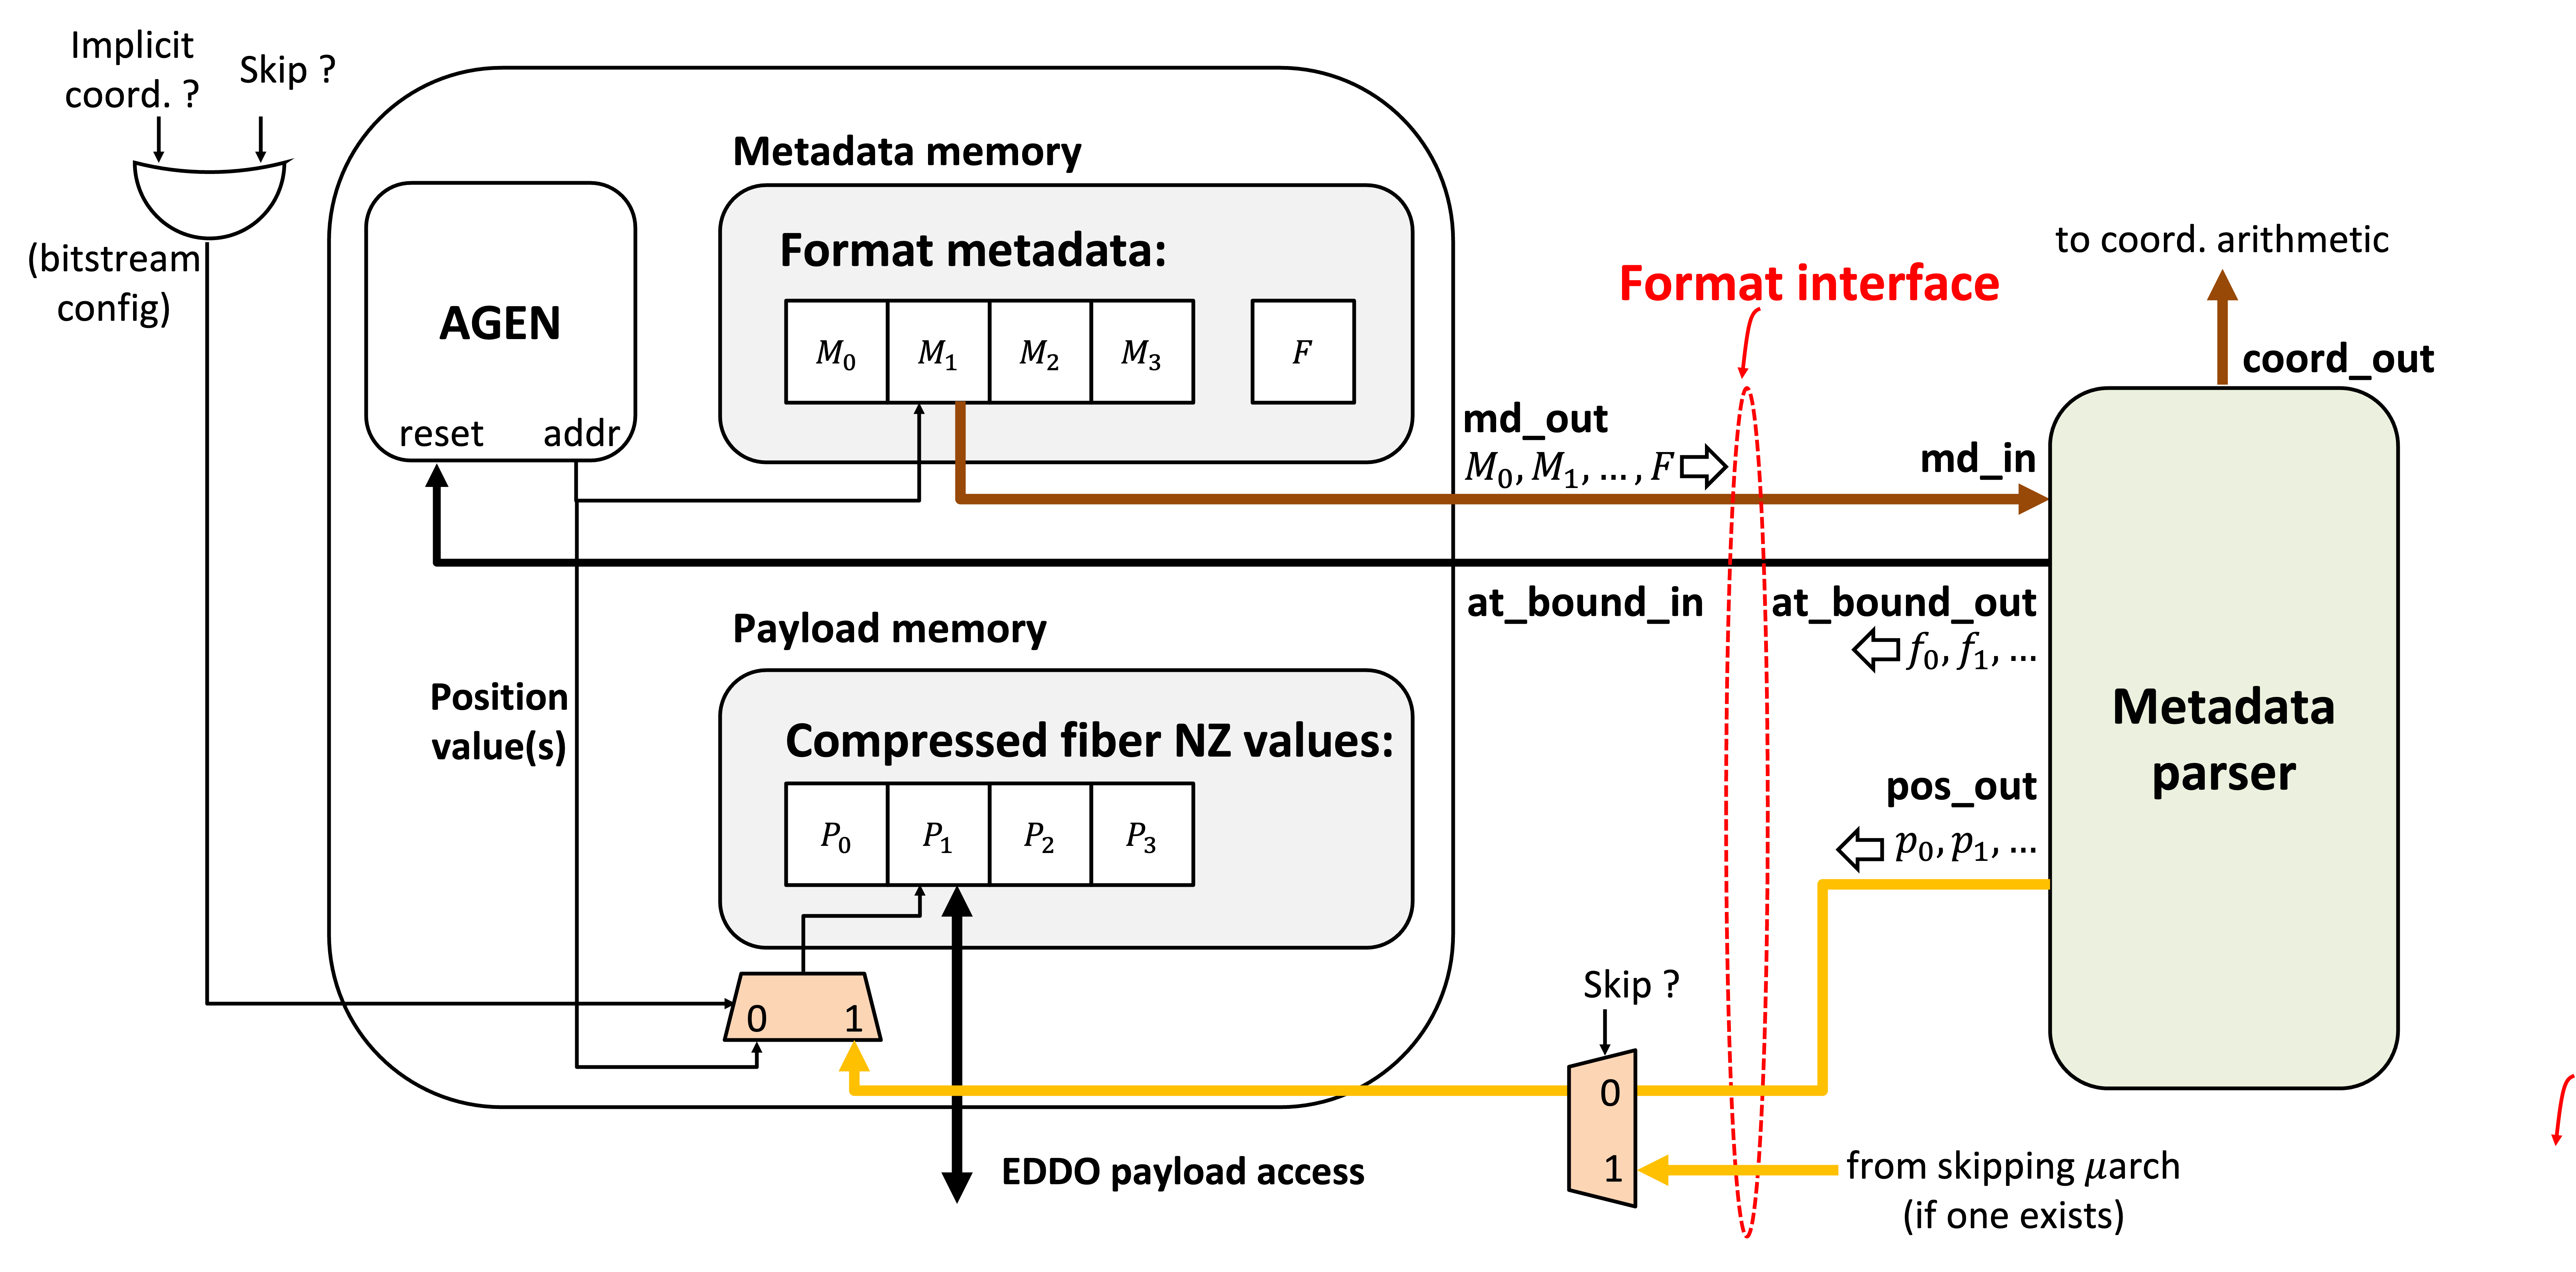
\includegraphics[width=0.95\textwidth]{figures/single_rank_general_format_smartbuffer_model.png}
    \caption{Sparse smartbuffer model for a single rank, supporting general sparse tensor formats. ${M_i}$ are general sparse metadata values, which may not be explicit coordinates. The metadata parser can orchestrate payload reads (via pos\_out) if this is enabled in the configuration bitstream. This is necessary for implicit coordinate representation formats. If skipping is enabled in the configuration bitstream, a skipping microarchitecture's output position stream can orchestrate payload reads. The functionality of the at\_bound\_out signal is unchanged. }
    \label{fig:single_rank_general_format_smartbuffer_model}
\end{figure}

There are a few problems with trying to apply the design in Figure~\ref{fig:single_rank_explicit_coordinate_smartbuffer_model} to a B-formatted fiber:

\begin{itemize}
    \item While B still stores the compressed fiber payloads as a series of consecutive non-zero/non-empty elements, the B-format metadata array always has a length equal to the dense length of the fiber's underlying rank, regardless of the number of non-zeroes. This prevents the AGEN from trivially co-iterating through the format-metadata and compressed-NZ-values arrays, as was done in Section~\ref{sec:single_explicit_fiber}.
    \item The B-format metadata may not be \textit{directly} utilized to lookup into the compressed-NZ-values array, as the metadata does not explicitly contain positional offsets that can be used for the lookup. 
\end{itemize}

In order to even look up into the compressed-fiber-NZ values, Figure~\ref{fig:single_rank_general_format_smartbuffer_model} shows that a different design is required which allows the metadata parser to process the B-format metadata into positional offsets and then request lookups into the compressed-fiber-NZ-values array. It is clear from Figure~\ref{fig:single_rank_general_format_smartbuffer_model} that the format interface bundle described in Section~\ref{sec:single_explicit_fiber} must be augmented with an additional input wire, which can receive requests from the metadata parser to lookup payloads in the compressed-fiber-NZ-values array.

\paragraph{Skipping.} 

\subsubsection{Multi-rank-pipelined (hierarchical), general-format sparse smartbuffer model}

\begin{figure}[ht]
    \centering
    \includegraphics[width=0.95\textwidth]{figures/hierarchical_general_format_sparse_smartbuffer.png}
    \caption{A sparse smartbuffer that stores a multi-rank tensor, inspired by the ExTensor\cite{extensor} design for traversing and intersecting deep fibertrees. The format microarchitecture implements a rank-parallel metadata processing pipeline. See Figure~\ref{fig:format_interface} for the structure of the format interface I/O bundle.}
    \label{fig:hierarchical_general_format_sparse_smartbuffer}
\end{figure}

\begin{figure}[ht]
    \centering
    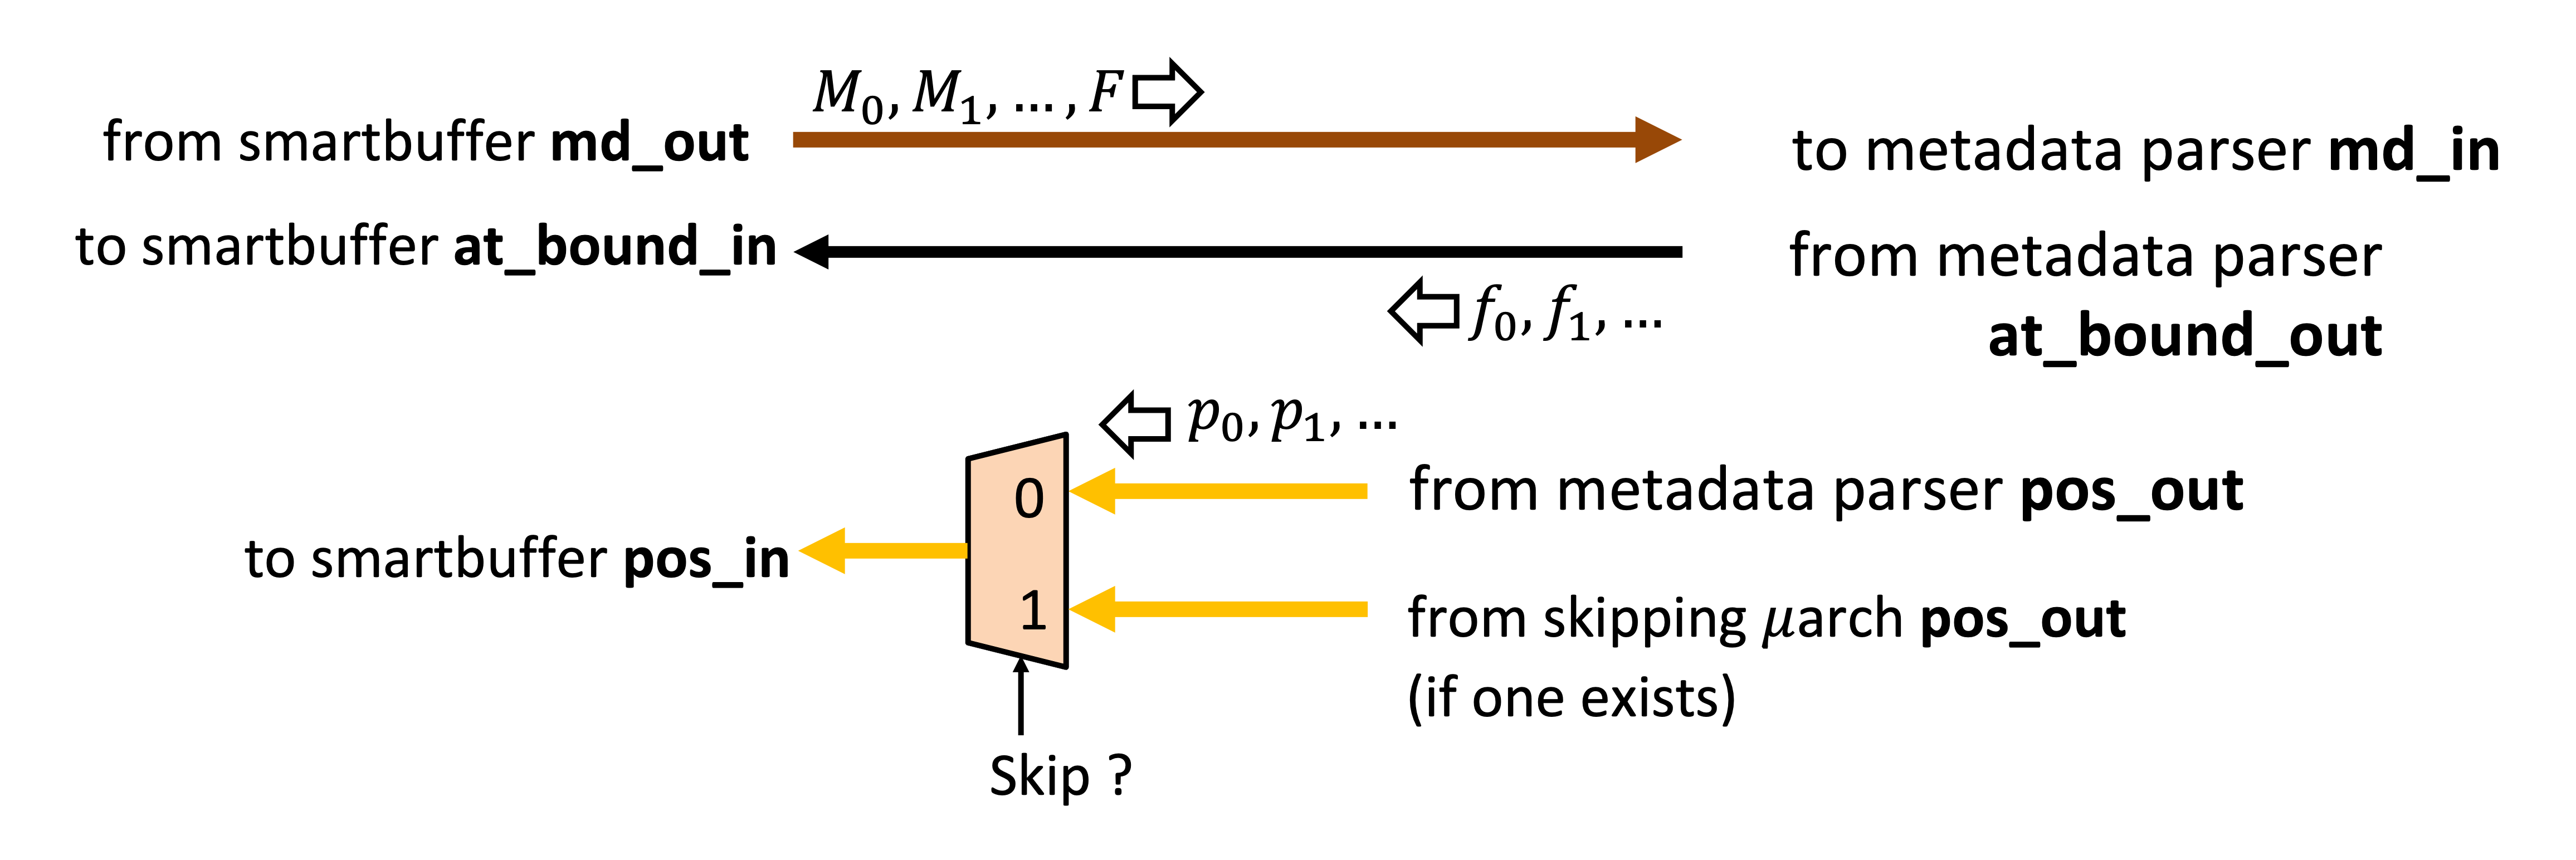
\includegraphics[width=0.95\textwidth]{figures/format_interface.png}
    \caption{Format interface I/O bundle. Sparse metadata moves from md\_out to md\_in. Payload lookup address offsets move from pos\_out to pos\_in. at\_bound\_out signals that fiber traversal is complete. The MUX that switches pos\_in between the metadata parser and the skipping microarchitecture is technically not part of the I/O bundle but is included for clarity and context.}
    \label{fig:format_interface}
\end{figure}

\subsection{Component parameterization}



\section{Integrating prior work}

\section{Overview of conceptual framework proposed in this work}

\begin{figure}[ht]
    \centering
    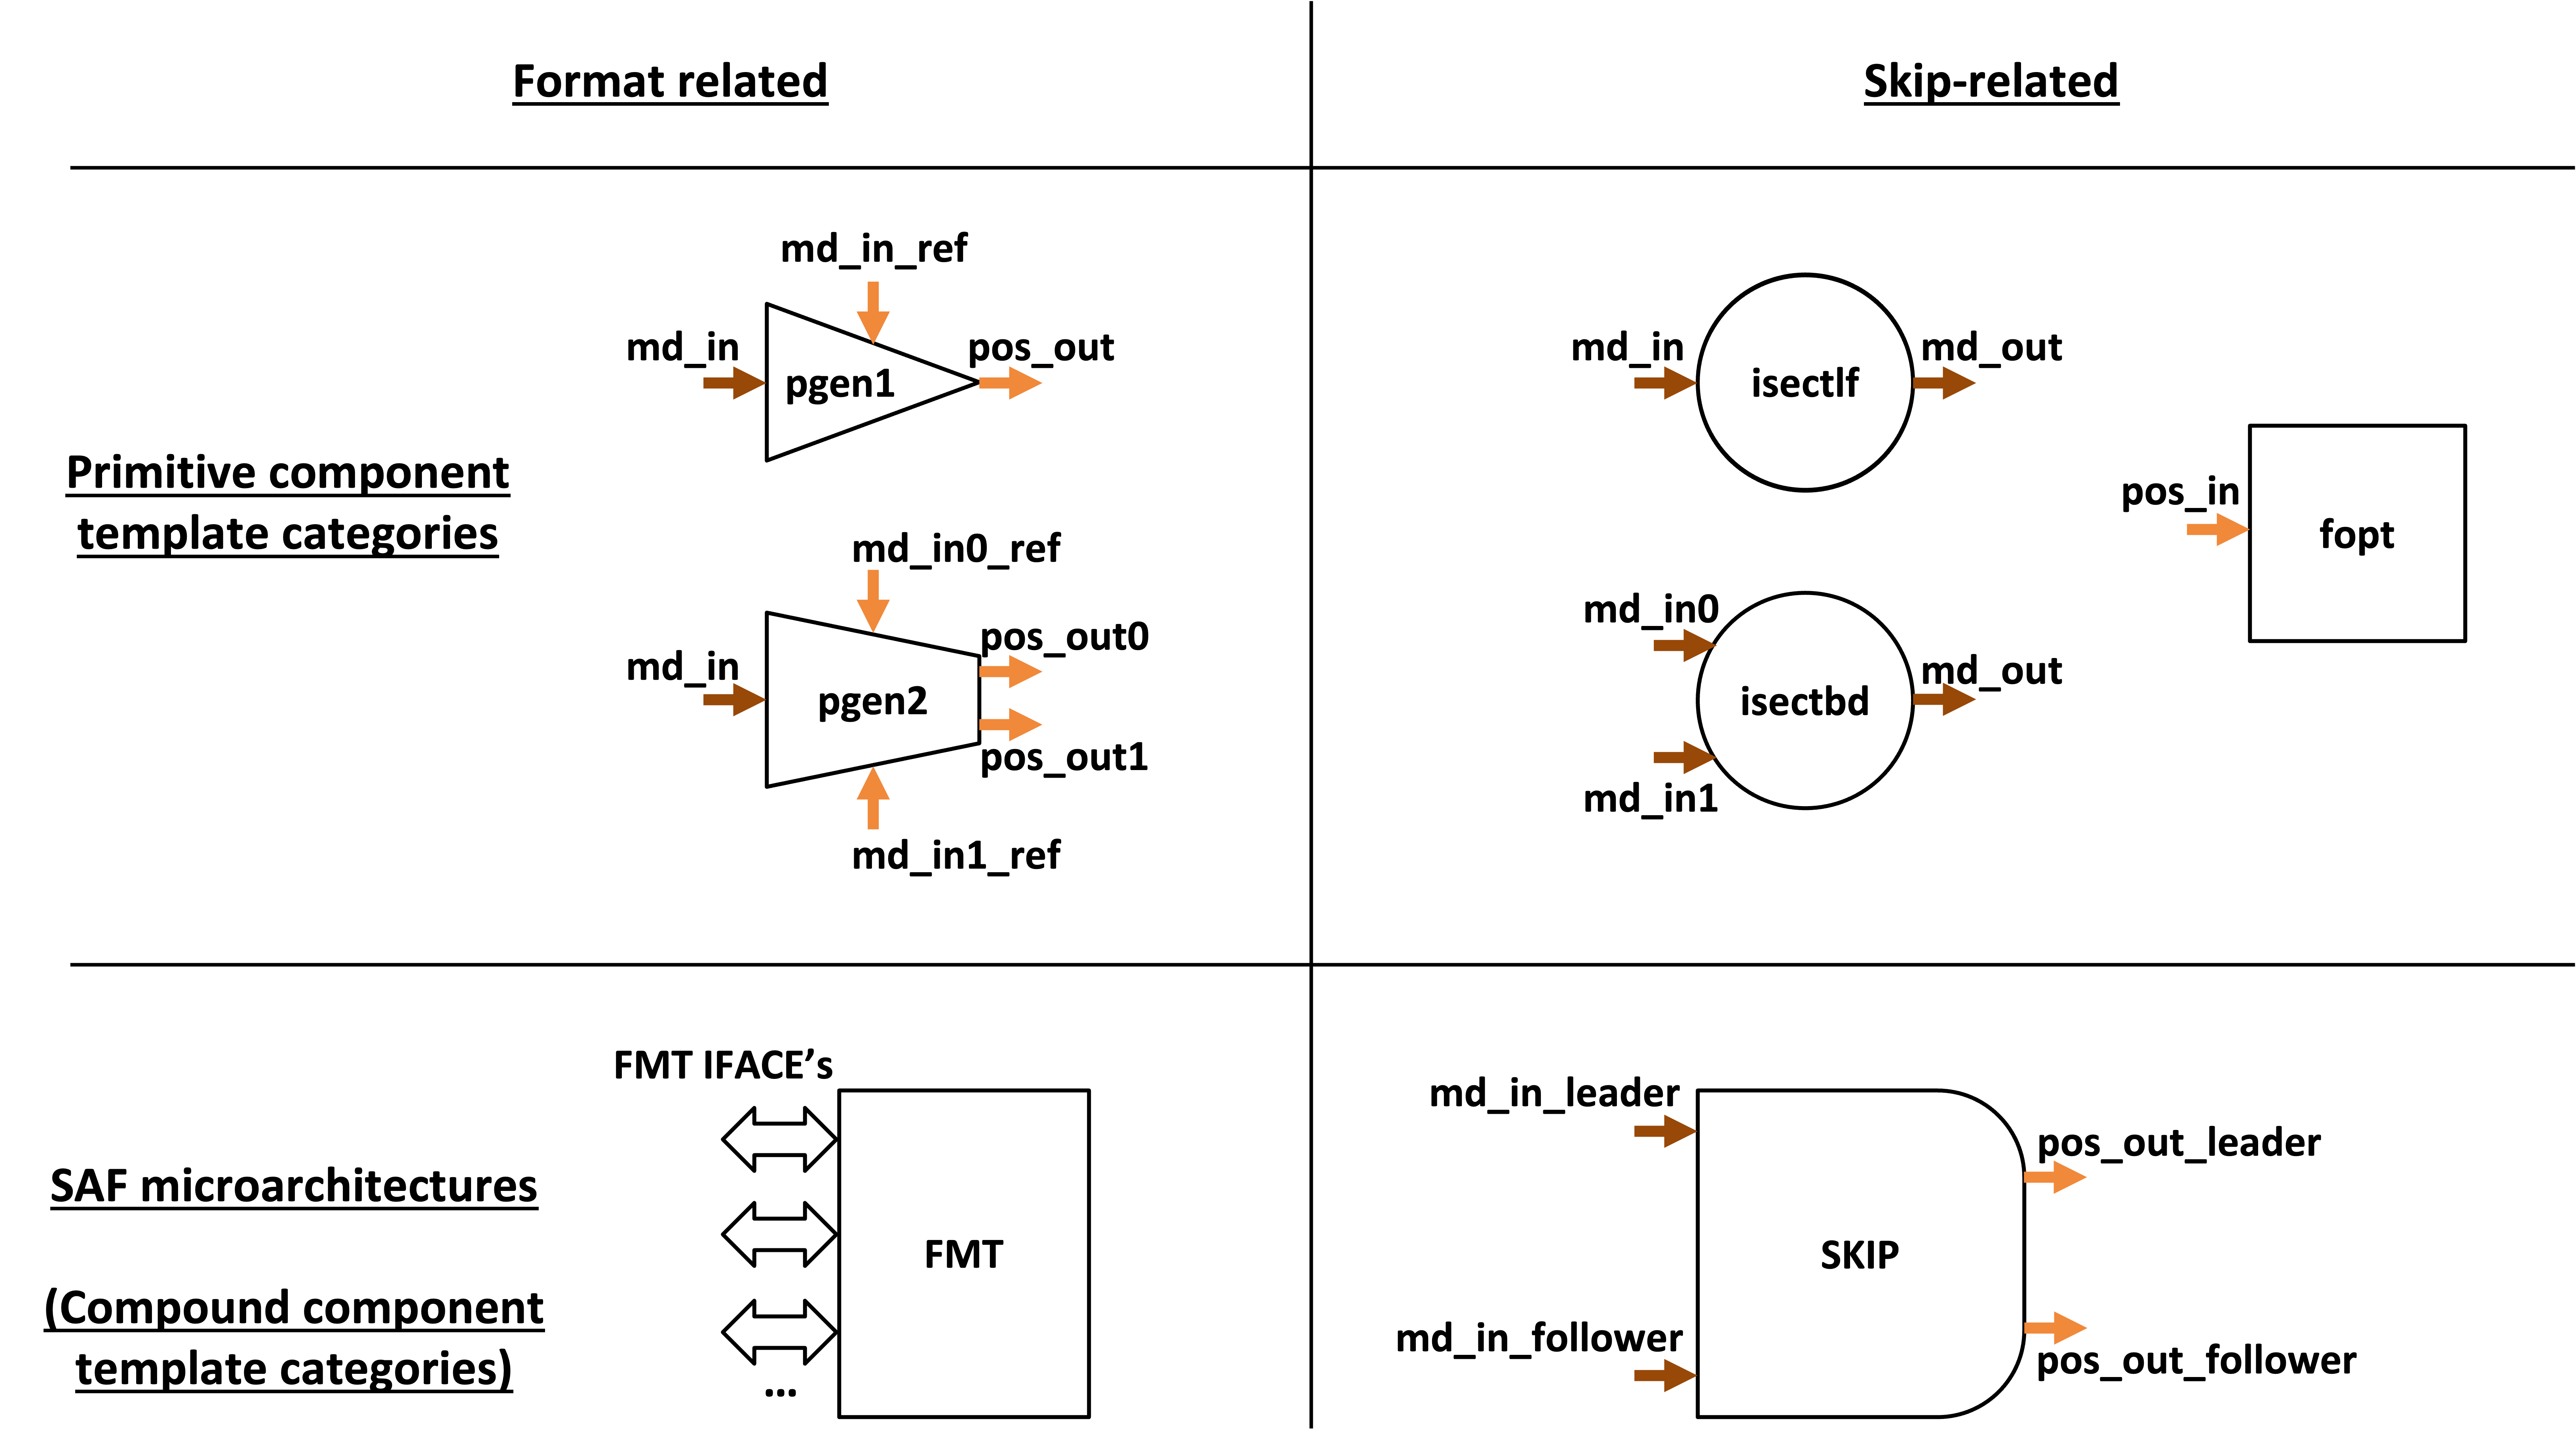
\includegraphics[width=0.95\textwidth]{figures/this_work_taxo.png}
    \caption{Overview of the SAF microarchitecture taxonomy developed in this work.}
    \label{fig:this_work_taxo}
\end{figure}


\chapter{RTL blocks}
\label{chapter:rtl}

This section introduces the RTL modules or ``RTL blocks'' which were developed and characterized for this work. The characterization \textit{process} will be discussed in Section~\ref{chapter:framework}.

\section{Scalar RTL blocks}

This work provides characterized RTL blocks for:

\begin{itemize}
    \item Arithmetic

    \begin{itemize}
        \item Adder
        \item Subtractor
        \item Multiplier
    \end{itemize}
    
    \item Comparison

    \begin{itemize}
        \item Equality comparator
    \end{itemize}
\end{itemize}

These straightforward circuits are useful as building blocks for other RTL designs, and the characterization metrics for these circuits are useful building-blocks for modeling.

These components are all parameterized by \textbf{operand bitwidth}. All of these components are scalar, processing one operand (or pair of operands) per cycle and producing one output.

\section{Vectorized RTL blocks}

All ``vectorized' RTL blocks consume vector inputs and yield vector outputs. Depending on implementation, the degree of input and output vectorization may be determined by separate parameters (as is the case for the ``skip-ahead'' intersection unit) or by a single parameter (as is the case for the two-fingered merge-based intersection unit.)

Here, ``vectorization'' is used to mean that (1) the input and output data structures of the RTL block are vectors, and (2) the processing throughput is such that all vector operands are consumed within a cycle, and each vector output is produced in its entirety within a cycle.

Notably, an RTL block being ``vectorized'' is decoupled from the degree of parallelism of the underlying combinational logic. The vectorized ripple prefix-sum, for example, uses a linear-depth design based on chained adders in order to process a vector of inputs within a cycle (provided that the critical path latency complies with the clock latency), while the vectorized parallel Kogge-Stone\cite{koggestone} prefix-sum uses a log-depth tree design that trades off higher area for sub-linear critical path length scaling.

\subsection{Vector pipelining and combinational unrolling}

Some RTL blocks such as prefix-sum naturally consume a vector and output a vector.

However, other blocks such as coordinate-payload intersection units and priority encoder, consume a vector and output a single value. A method is needed to increase the throughput of these components in cases where one-result-per-cycle is insufficient.

Previous works such as ExTensor\cite{extensor} rely on vector pipelining in order to increase the throughput of intersection units. Although the structure of the vector pipeline is not laid out explicitly, one can imagine how such a vector pipeline might be implemented: first implement a single stage which is equivalent to one ``step'' of the intersection process; the stage should accept a state vector representing the progress toward completing the intersection, and should output (1) at most one and at least zero matches which were discovered by the stage, and (2) an updated state vector. Second, cascade multiple stages, such that the output of the cascade is an updated state vector reflecting \textit{multiple} stages of the intersection process, as well as potentially multiple intersection matches which were discovered.

In the context of this work, two ways of creating staged RTL are relevant:

\begin{itemize}
    \item \textbf{Vector pipelining.} Multiple stages are daisy-chained but separated by registers; each pipeline stage is a single intersection stage. \textbf{Propagation delay requirement:} the propagation delay of a single stage must be less than the clock period, minus margin.
    \item \textbf{Combinational unrolling.} Multiple stages are daisy-chained and \textbf{combinationally-connected without pipeline registers}; the whole multi-stage intersection unit constitutes a single pipeline stage. \textbf{Propagation delay requirement:} the propagation delay \textbf{of the whole multi-stage intersection unit} must be less than the clock period, minus margin.
\end{itemize}

The benefit of vector pipelining is the more lenient propagation delay requirement; empirically, a more lenient propagation delay requirement appears to also results in lower power consumption and area per-stage after gate-level synthesis.

The benefits of combinational unrolling are that (1) the energy and area overhead of pipelining registers avoided, and (2) there is no need orchestrate control signals between pipeline stages. However, besides the propagation delay, an additional drawbacks is that combinational unrolling can have non-linear overheads resulting from i.e. the logic which compacts the matches found by multiple intersection stages into a single vector.

In this work, each RTL block is parameterized, and then characterized over a range of \textbf{combinational unrolling} depths, starting at 1. In future work it could be valuable to explore vector pipelining as well.

\subsubsection{Chaining}

As described above, vector pipelining and combinational unrolling are implemented here in such a way that each stage is identical, and an updated state vector is passed from stage to stage.

What if an operation such as intersection is not completed in a single pass through the vector pipeline/combinational intersection unit? There is nothing to prevent \textit{chaining}, i.e. collecting the state vector at the output of the vector pipeline/combinational intersection unit, and feeding it back to the input. 

With chaining, the size of the vector pipeline/combinational unrolling does not affect the feasibility of a computation, only its runtime.

\subsection{Prefix-sum units}

Prefix sum does not require vector pipelining or combinational unrolling.

\textbf{Vectorized prefix sum parameters:}

\begin{itemize}
    \item Input vector length
    \item Word bits
\end{itemize}

\textbf{RTL implementations for the following prefix sum designs (all sharing the above parameter list) are provided:}

\begin{itemize}
    \item \textbf{Ripple prefix-sum:} linear-depth prefix-sum implementation based on chained adders.
    \item \textbf{Parallel Kogge-Stone\cite{koggestone} prefix-sum:} log-depth prefix-sum implementation based on adder trees.
\end{itemize}

\subsubsection{Kogge-Stone prefix-sum}

\begin{figure}[H]
    \centering
    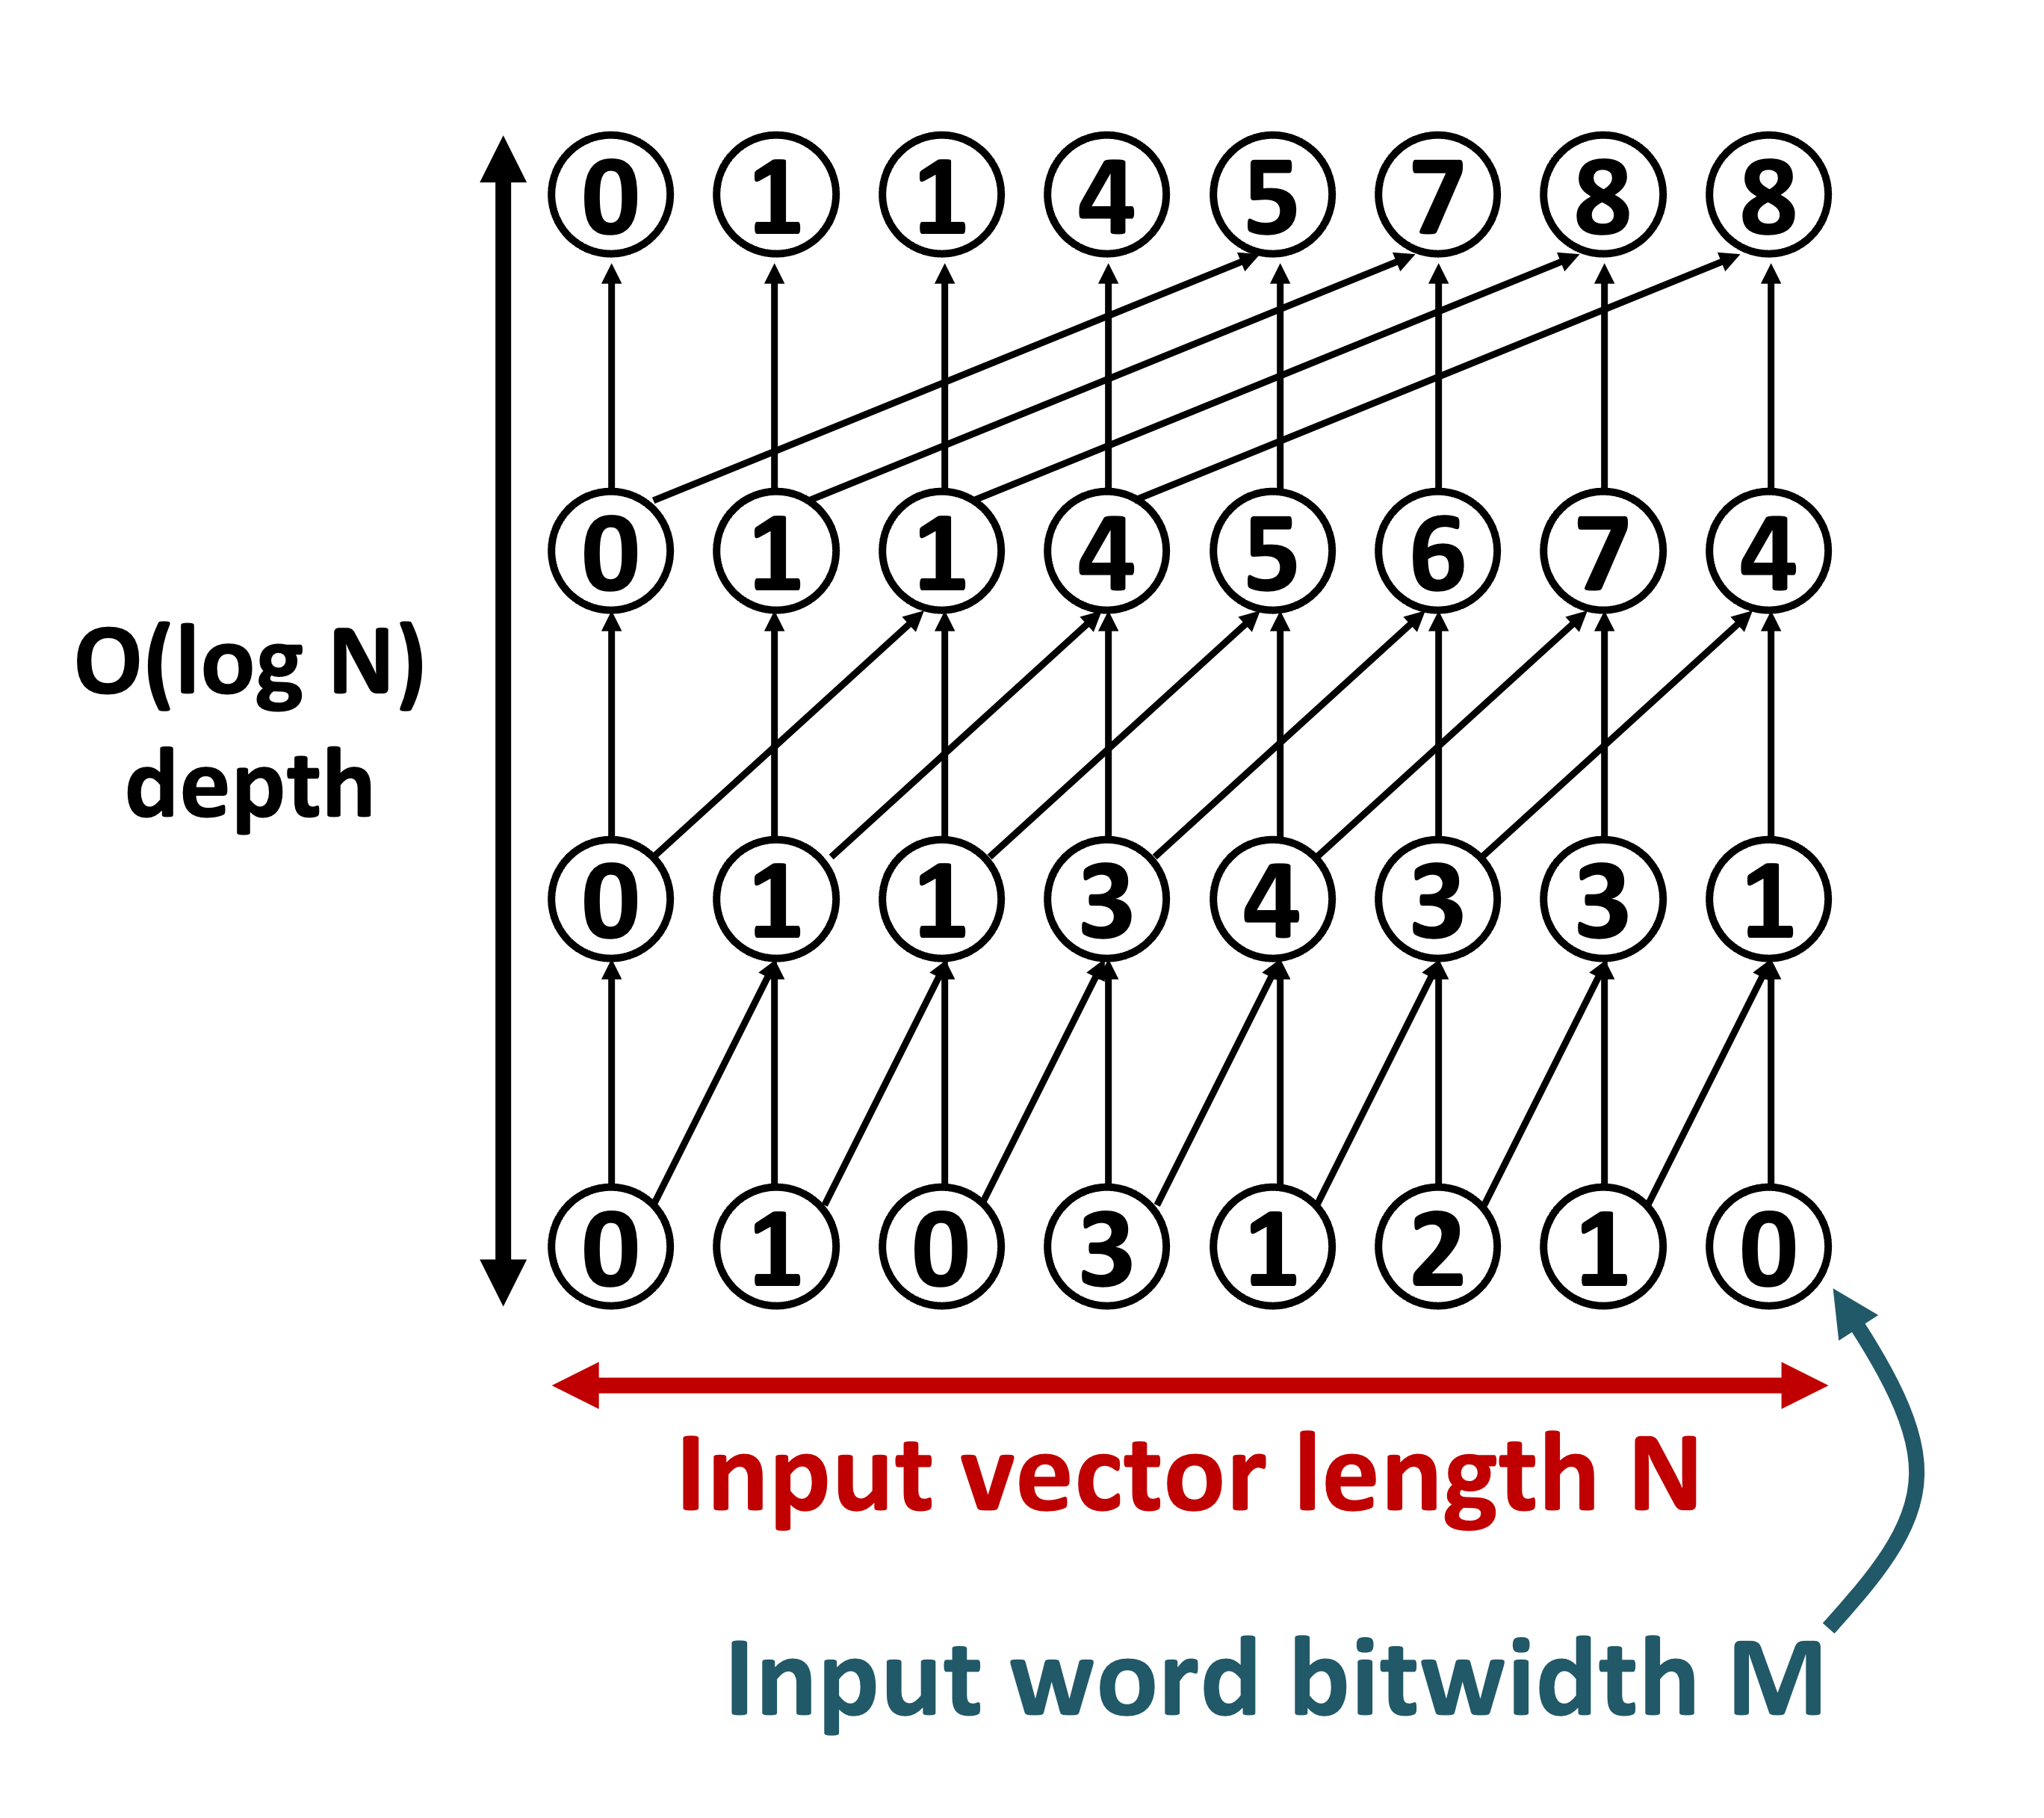
\includegraphics[width=0.95\textwidth]{figures/kogge_stone_prefix_sum.png}
    \caption{The Kogge-Stone\cite{koggestone} prefix-sum RTL block implements a log-depth vectorized prefix-sum with a 1-stage vector pipeline (registered I/O.) It is parameterized by \textbf{input word bitwidth} and \textbf{degree of vectorization.}}
    \label{fig:kogge_stone_prefix_sum}
\end{figure}

Figure~\ref{fig:kogge_stone_prefix_sum} summarizes Kogge-Stone prefix-sum.

\subsubsection{Ripple prefix-sum}


\begin{figure}[H]
    \centering
    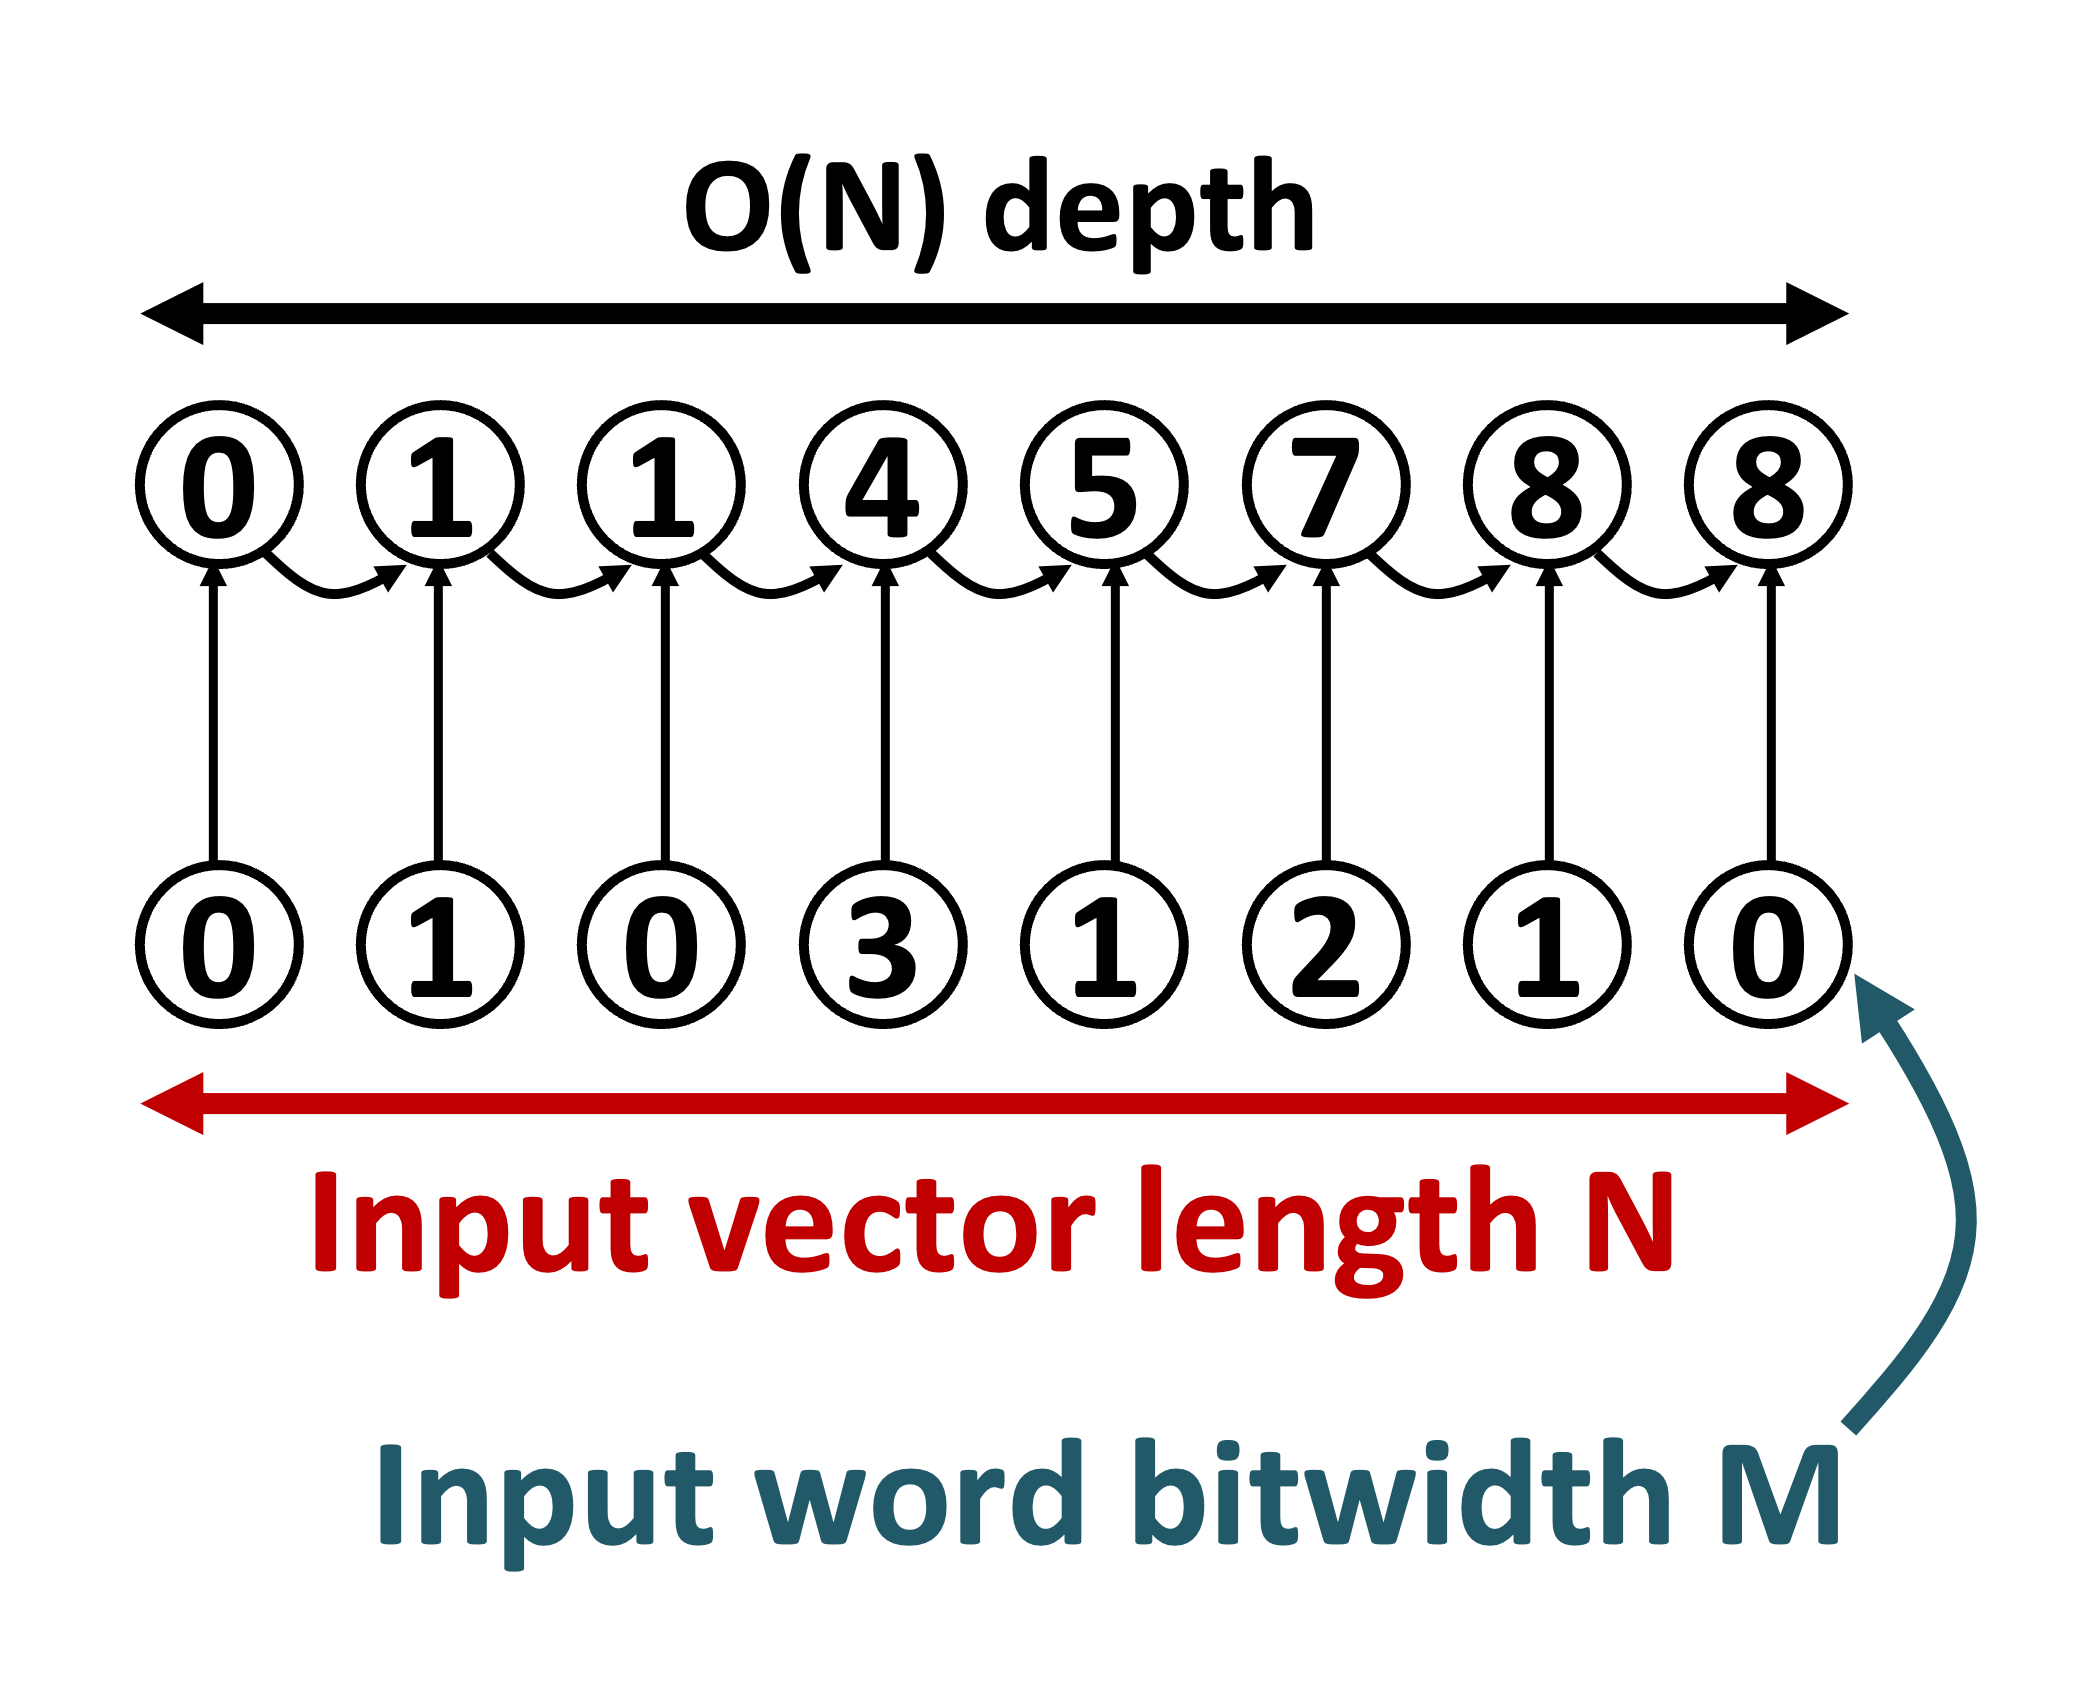
\includegraphics[width=0.95\textwidth]{figures/ripple_prefix_sum.png}
    \caption{The ripple prefix-sum RTL block implements a linear-depth vectorized prefix-sum. It is parameterized by \textbf{input word bitwidth} and \textbf{degree of vectorization.} This RTL block is implemented as a 1-stage vector pipeline (registered I/O) however the combinational design is not ``parallel'' and propagation delay is linear in the degree of vectorization.}
    \label{fig:ripple_prefix_sum}
\end{figure}

Figure~\ref{fig:ripple_prefix_sum} summarizes ripple prefix-sum.

\subsection{Priority encoder units}

Priority encoder requires either vector pipelining or combinational unrolling in order to support output throughput greater than 1.

\textbf{Vector priority encoder parameters:}

\begin{itemize}
    \item Number of input bits
    \item Output vector size
    
    \begin{itemize}
        \item Meaning: if the output vector size is $k$, a vectorized priority encoder returns a vector of indices for the top-$k$ priority hot bits in the input vector. 
        \item If the input bitmask contains $n < k$ hot bits, the priority encoder returns a length-$k$ vector with the $n$ hot-bit indices compacted into the first $n$ vector elements; vector elements at offsets $>n-1$ are undefined.
    \end{itemize}

\end{itemize}

\textbf{RTL implementations for the following priority encoder designs (all sharing the above parameter list) are provided:}

\begin{itemize}
    \item \textbf{Parallel decimation-by-2 priority encoder\cite{recursive_priority_encoder}:} log-depth, decimation-by-2 parallel priority encoder design.
\end{itemize}

\subsection{Intersection units}

Several intersection unit varieties are explored in this work:

\begin{itemize}
    \item ExTensor-like\cite{extensor} naive two-finger intersection
    \item ExTensor-like\cite{extensor} optimized intersection unit
    \item SparTen-like\cite{sparten} Bitmask intersection unit
    \item Direct-mapped intersection unit, a potentially novel intersection unit design developed for this work.
\end{itemize}

Both ExTensor-like intersection units require either vector pipelining or combinational unrolling in order to support output throughput greater than 1.

\subsubsection{Two-finger intersection unit (``ExTensor-naive-like'')}

% Radix-2 intersection overview figure
\begin{figure}[H]
    \centering
    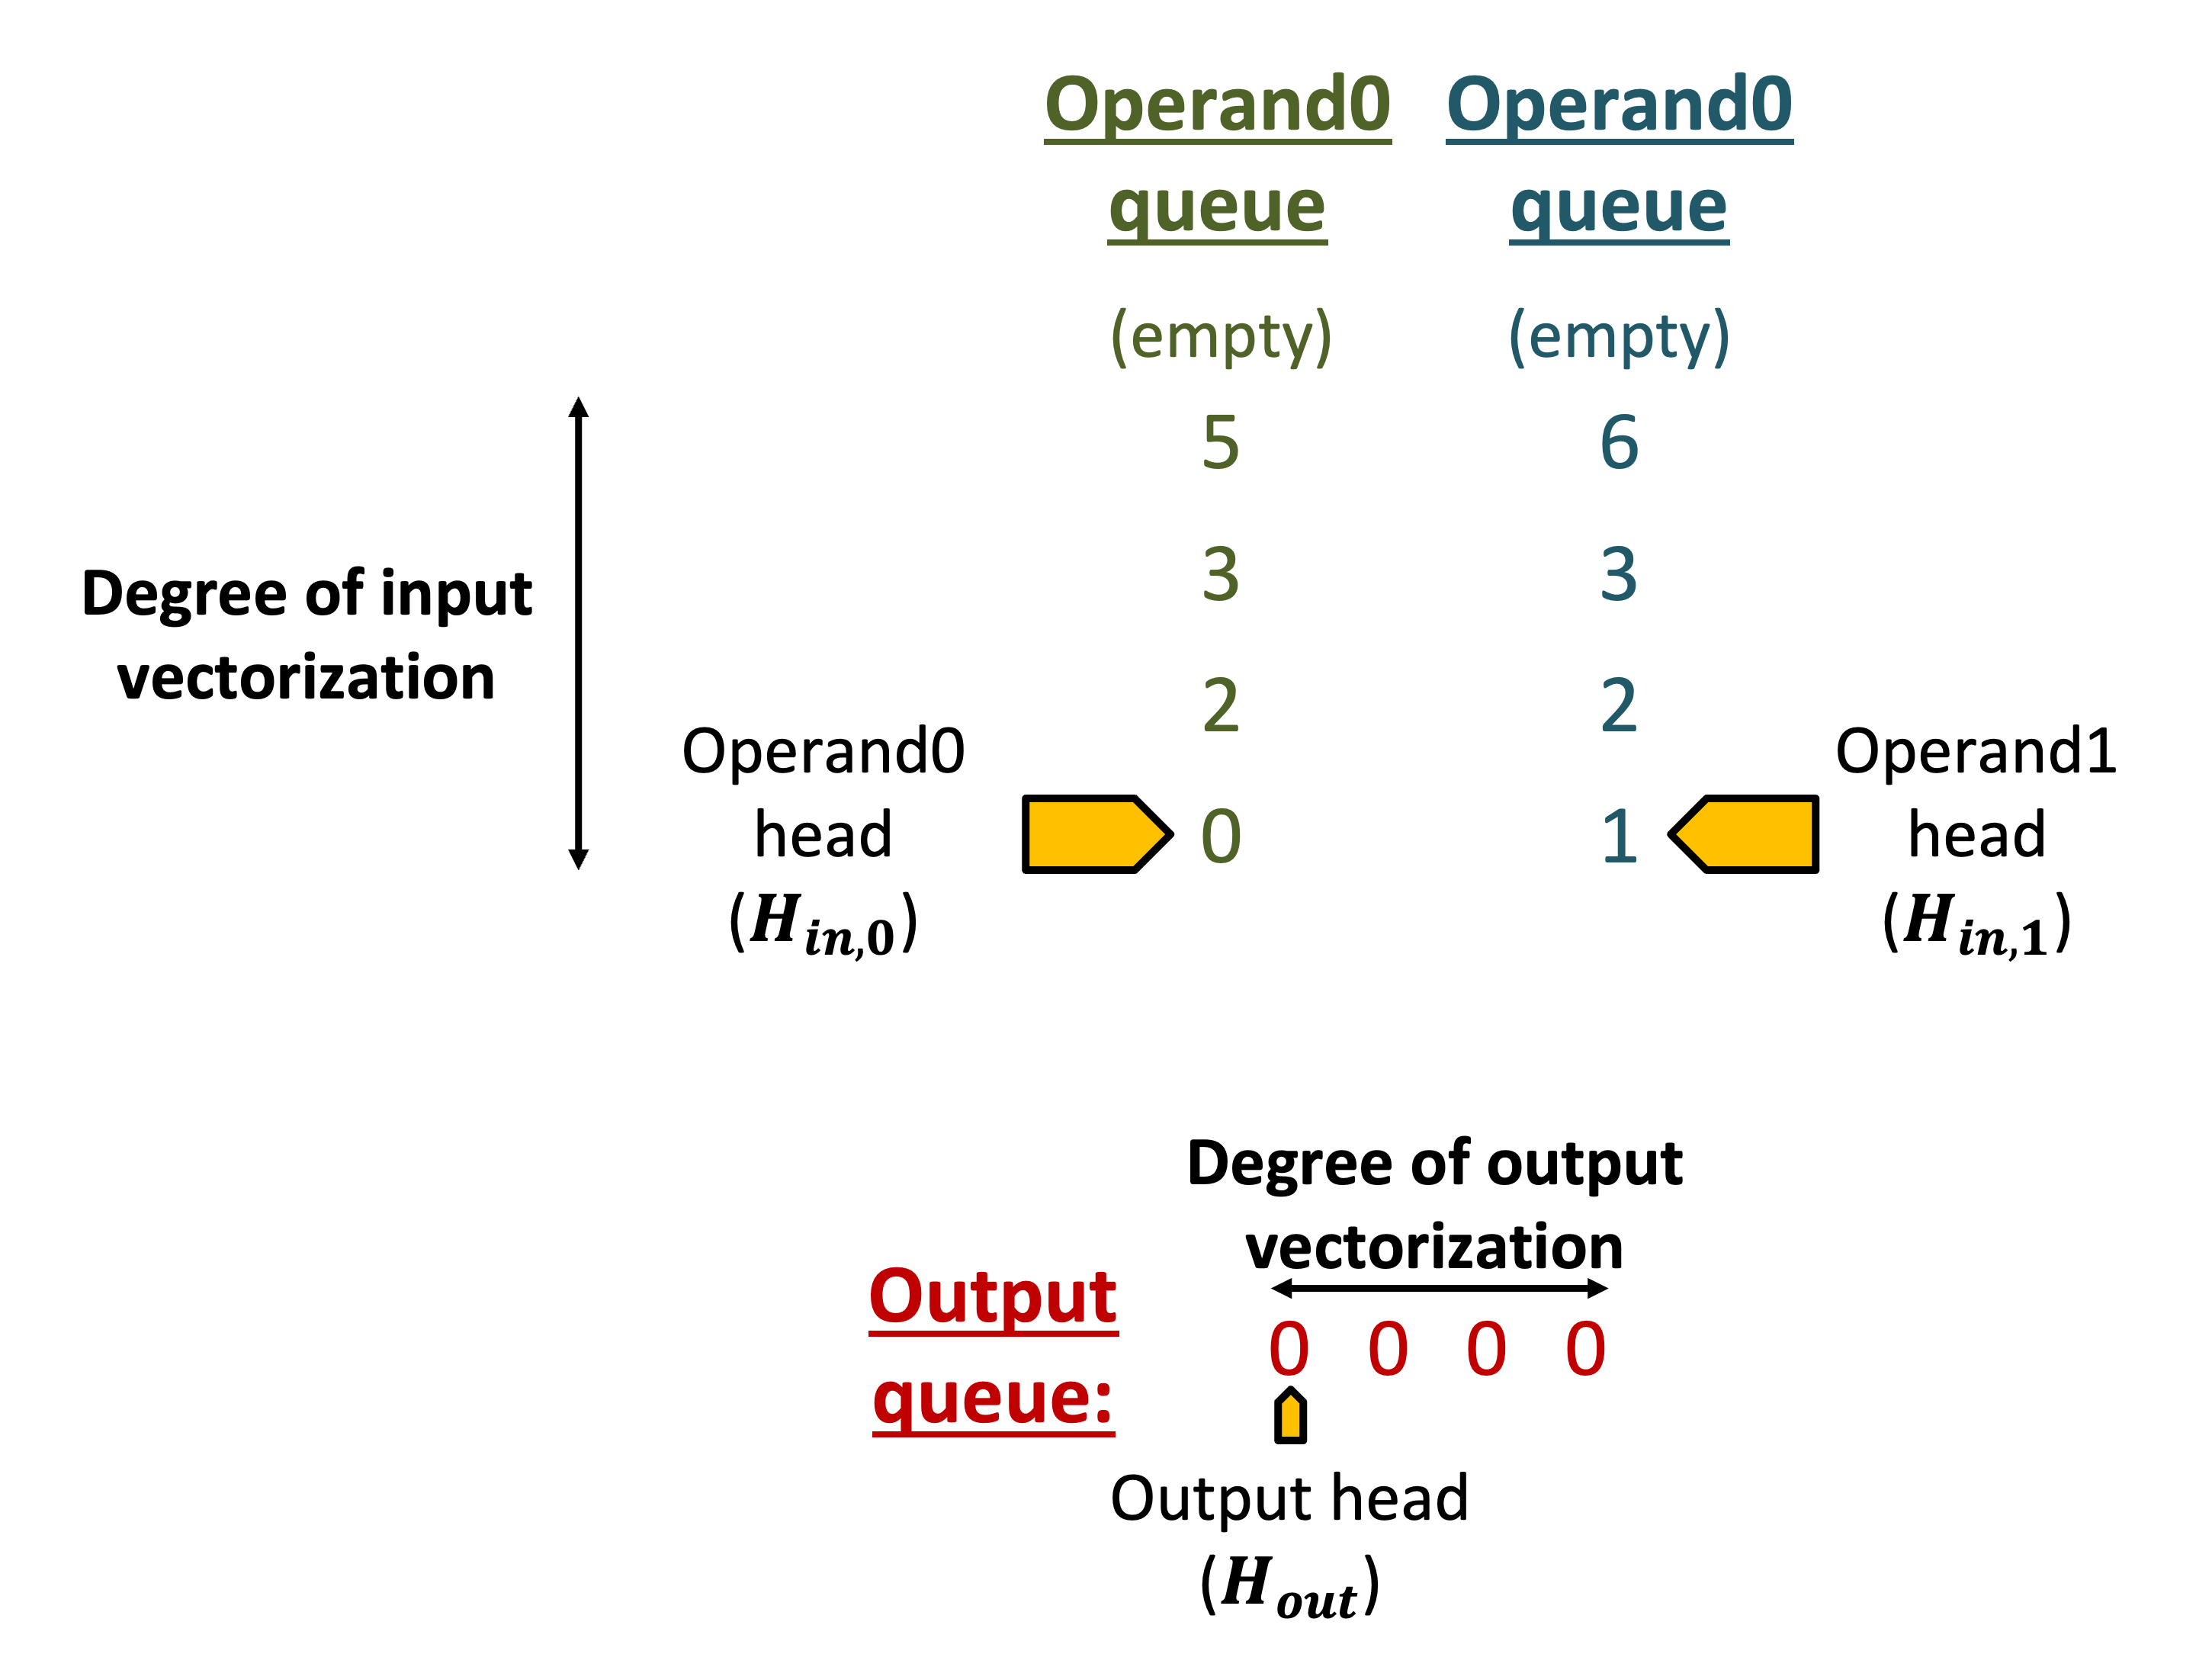
\includegraphics[width=\linewidth]{figures/radix2_intersect_overview.png}
    \caption{Overview of two-fingered intersection unit}
    \label{fig:radix2-overview}
\end{figure}

% Radix-2 intersection example figure
\begin{figure}[H]
    \centering
    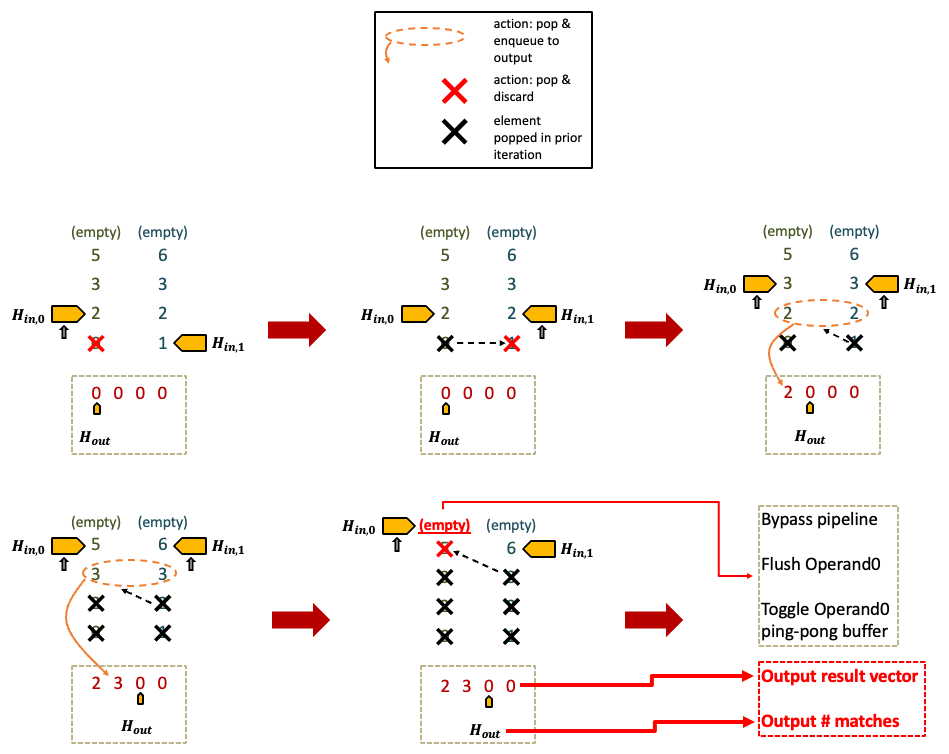
\includegraphics[width=\linewidth]{figures/radix2_intersect_example.png}
    \caption{Example of Radix2 Intersection}
    \label{fig:radix2-example}
\end{figure}

The two-finger intersection unit, modeled off of ExTensor\cite{extensor}, is similar to a radix-2 merge except it only outputs a value when the heads of the two lists are equal. This is exemplified in Figure~\ref{fig:radix2-overview} and Figure~\ref{fig:radix2-example}. Figure~\ref{fig:radix2-example} shows how the lowest element is popped for either vector, iteratively, until one or both vectors are empty. If the heads of the vectors are equal, both vectors are popped and the matching value is integrated into the output vector.

% Radix-2 intersection overview figure
\begin{figure}[H]
    \centering
    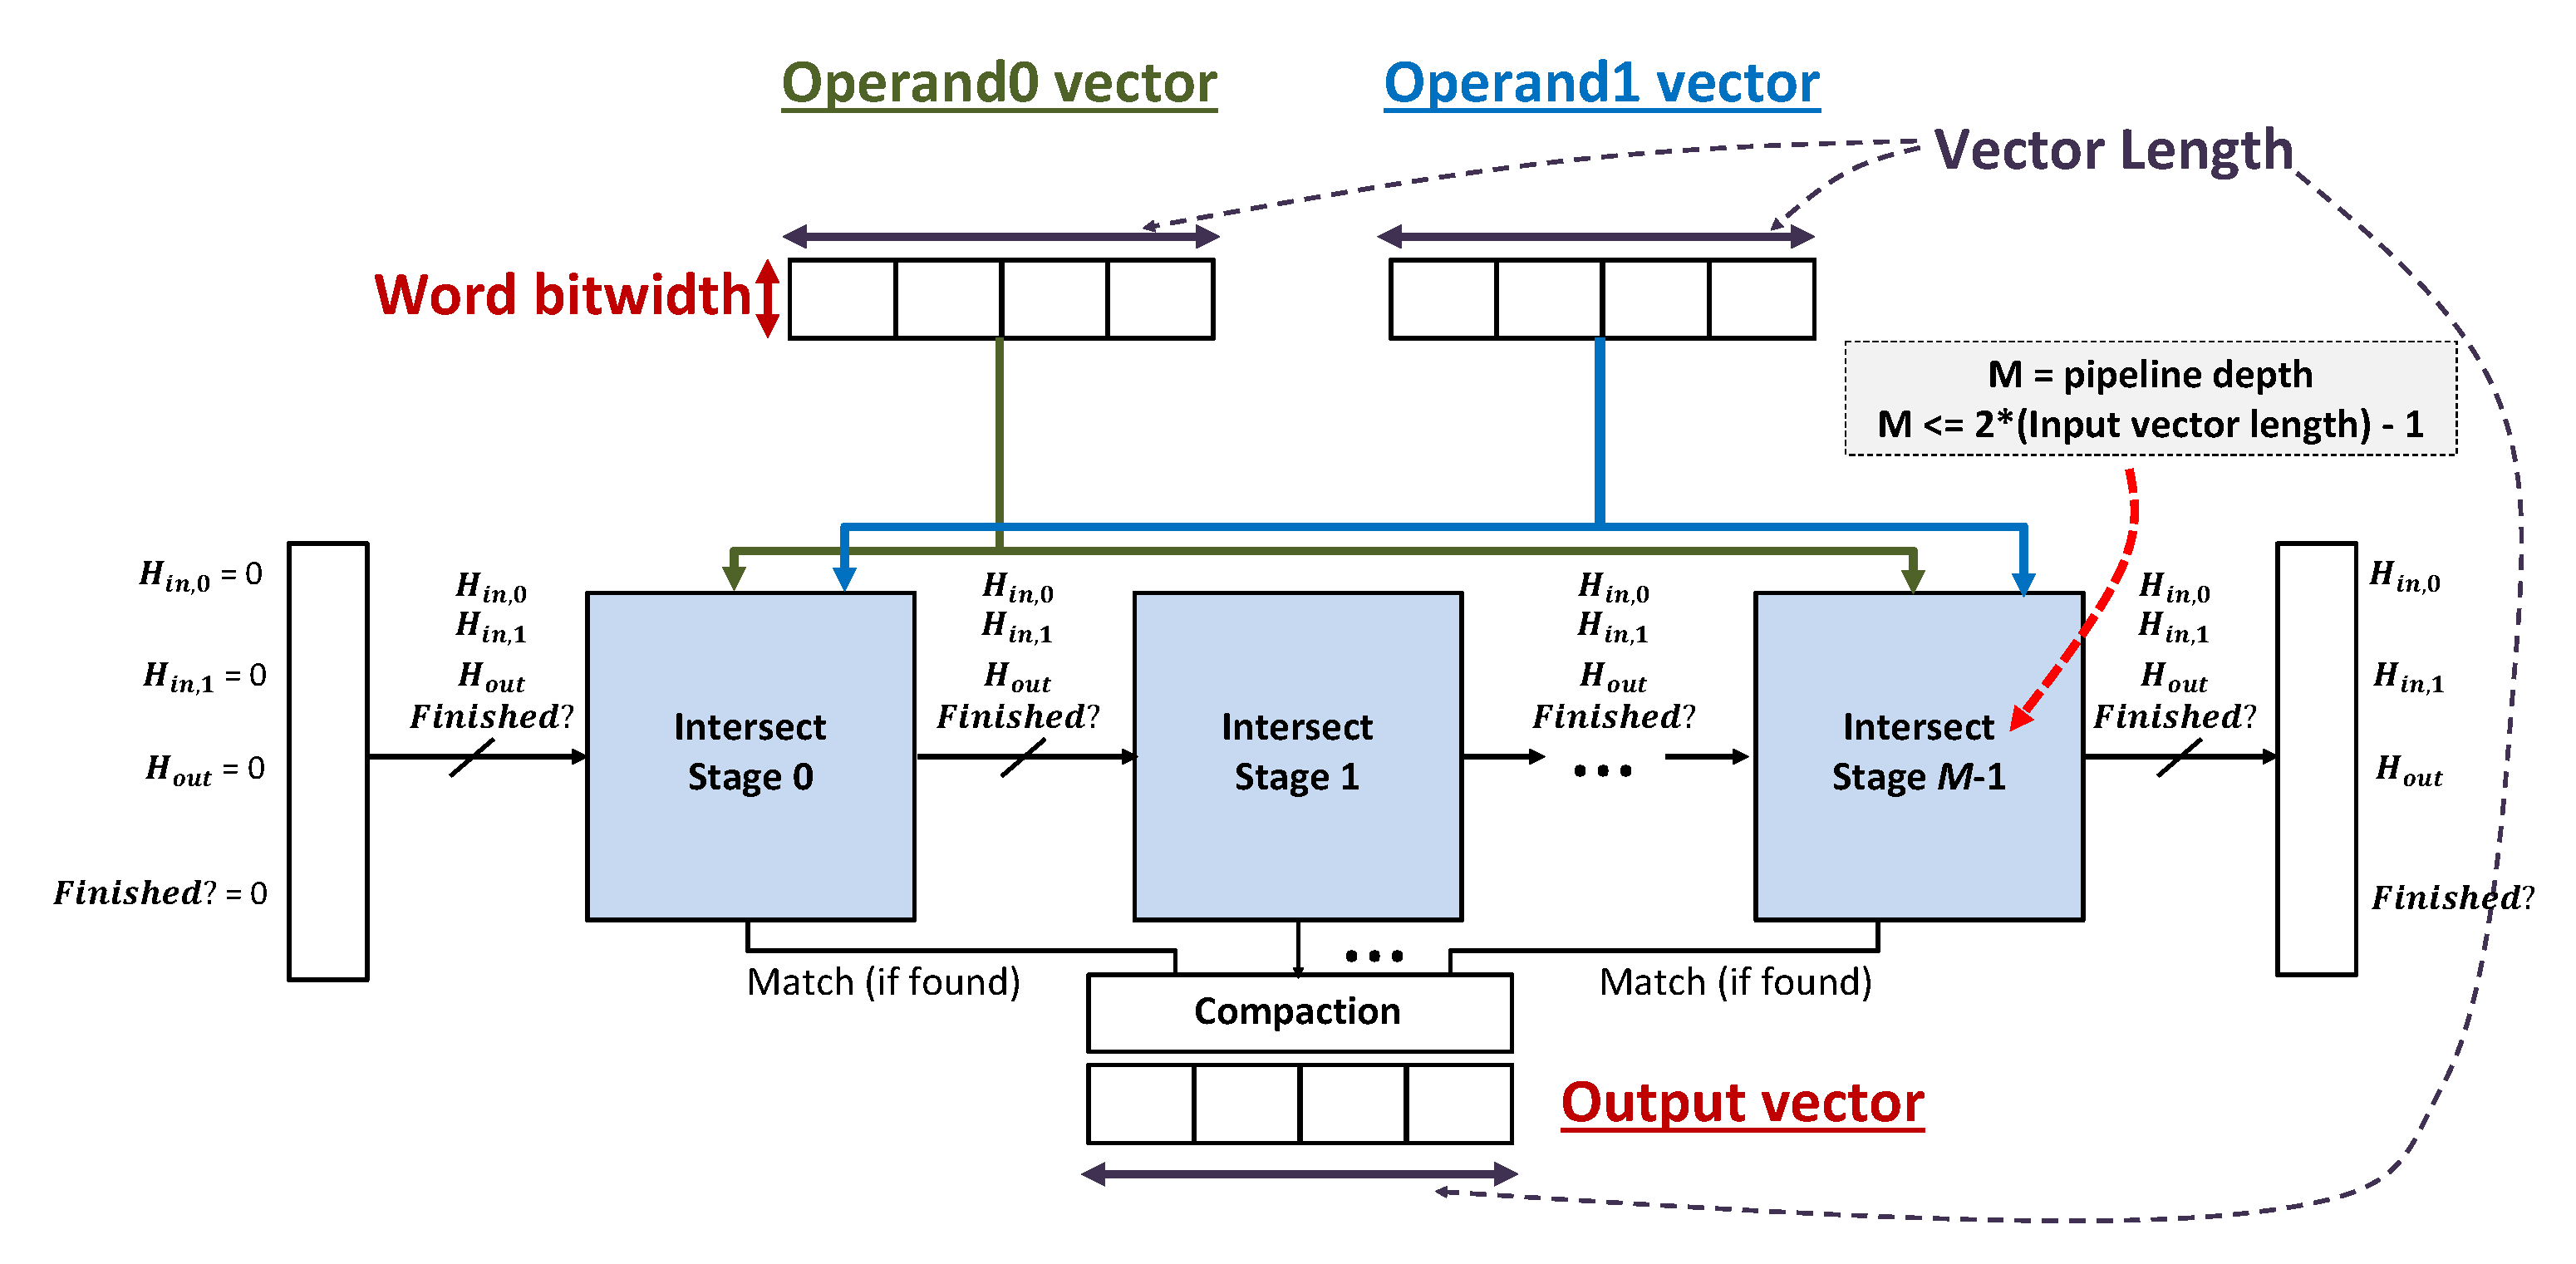
\includegraphics[width=\linewidth]{figures/two_finger_merge_pipeline.pdf}
    \caption{Two-fingered intersection vector pipelining or combinational unrolling.}
    \label{fig:radix_2_vector pipeline}
\end{figure}

Figure~\ref{fig:radix_2_vector pipeline} shows the approach to implementing vector pipelining or combinational unrolling for the two-fingered intersection unit. A stage vector enters the pipeline on the left, and an updated state vector exits on the right. The two operand vectors enter from above and are shared between each stage; in combinational unrolling, the need for multiple read/write ports can potentially lead to non-linear overheads. Special compaction logic compacts all matches from all stages into an output vector.

The state vector includes a ``Finished?'' signal, triggered when one or both lists are empty; when a stage raises this signal, all subsequent stages are bypassed.

\subsubsection{``Skip-ahead'' intersection unit (``ExTensor-optimized-like'')}

The skip-ahead intersection unit - also inspired by ExTensor\cite{extensor} - uses an optimized content-aware search process to increase the probability of finding an intersection match.

\begin{figure}[ht]
\centering
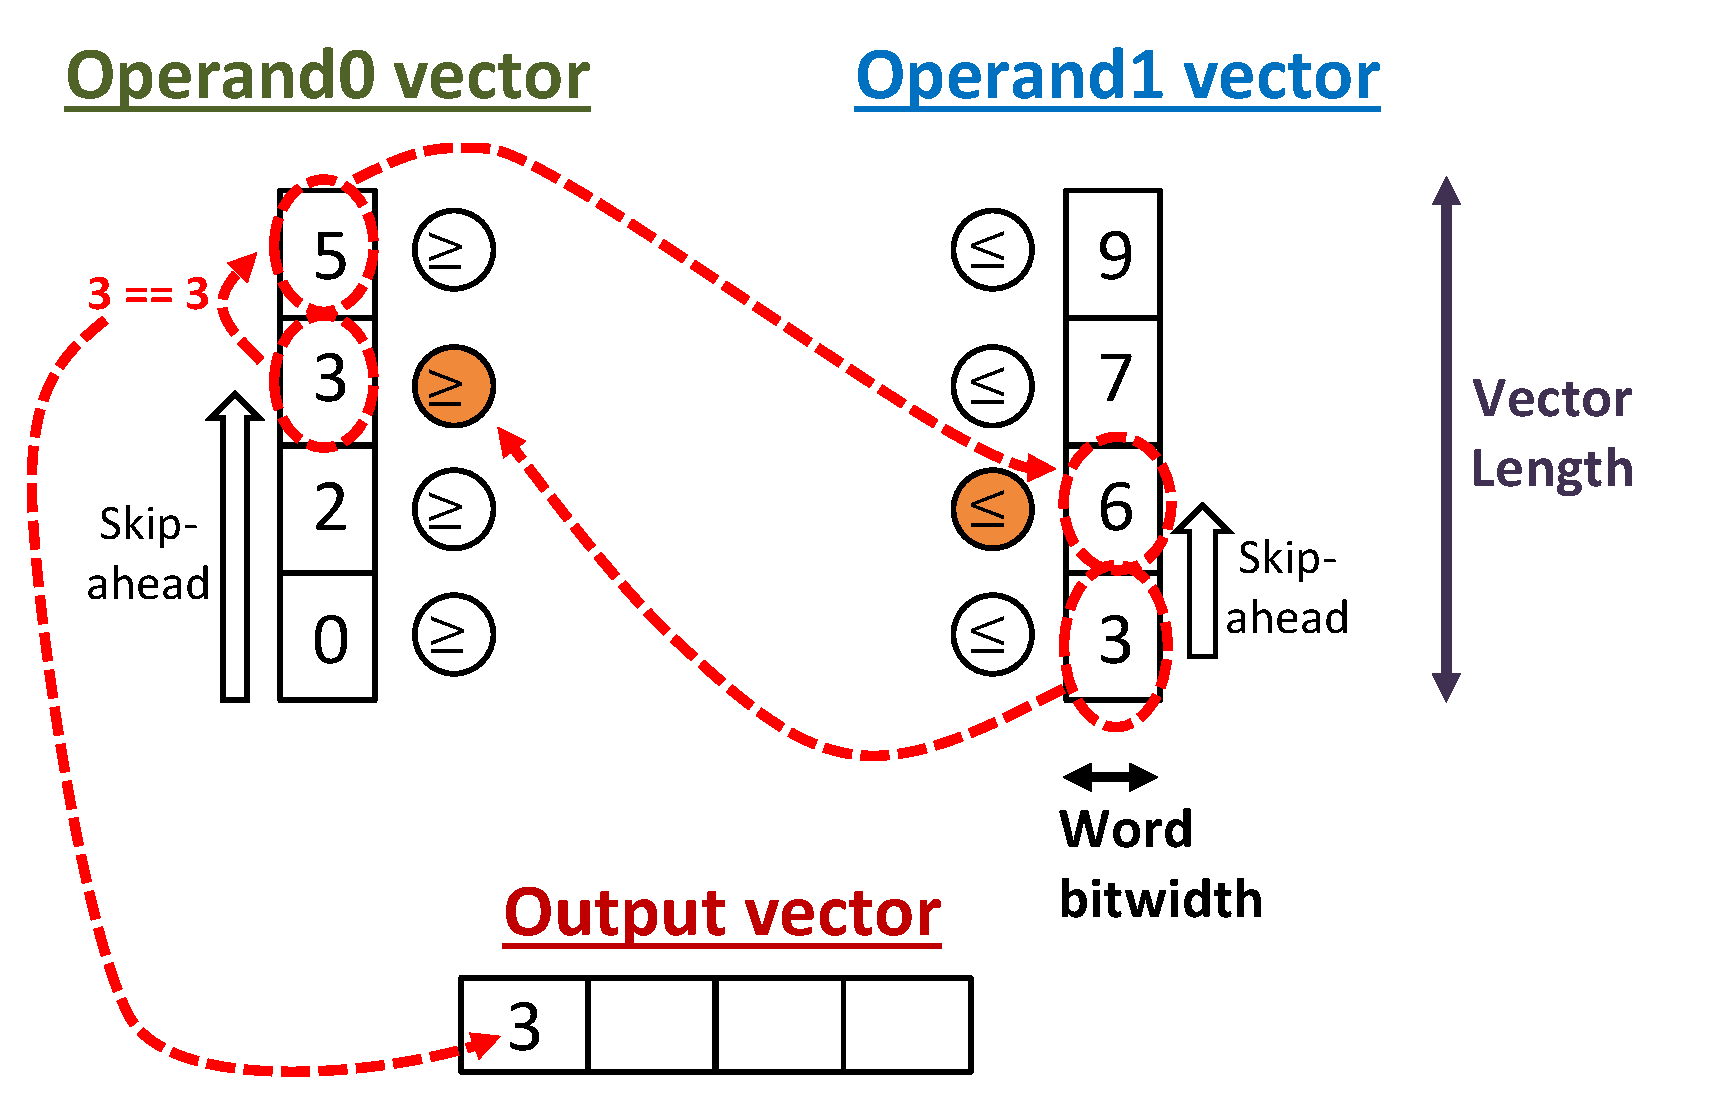
\includegraphics[width=0.7\textwidth]{figures/skip_ahead_dia.pdf}
\caption{.}
\label{fig:skip_ahead_dia}
\end{figure}

Figure~\ref{fig:skip_ahead_dia} illustrates how the content-aware search allows the intersection unit to ``skip-ahead'': by using content-addressable memories (CAMs), the control logic associated with the Operand1 vector can find the first element of Operand0 which is equal or greater than the head of Operand1, in a single step. 

Otherwise, the implementation of combinational unrolling/vector pipelining for skip-ahead intersection is identical to Figure~\ref{fig:radix_2_vector pipeline}.

\subsubsection{Parallel direct-mapped intersection unit}

The parallel direct-mapped intersection unit is a potentially novel intersection unit design developed for this work.

It finds all matches between two vectors in a single cycle, without pipelining or combinational unrolling.

This design intersects two vectors of sorted coordinate metadata, and outputs a third sorted vector of common metadata values between the two input vectors. 

\clearpage

\begin{figure}[H]
    \centering
    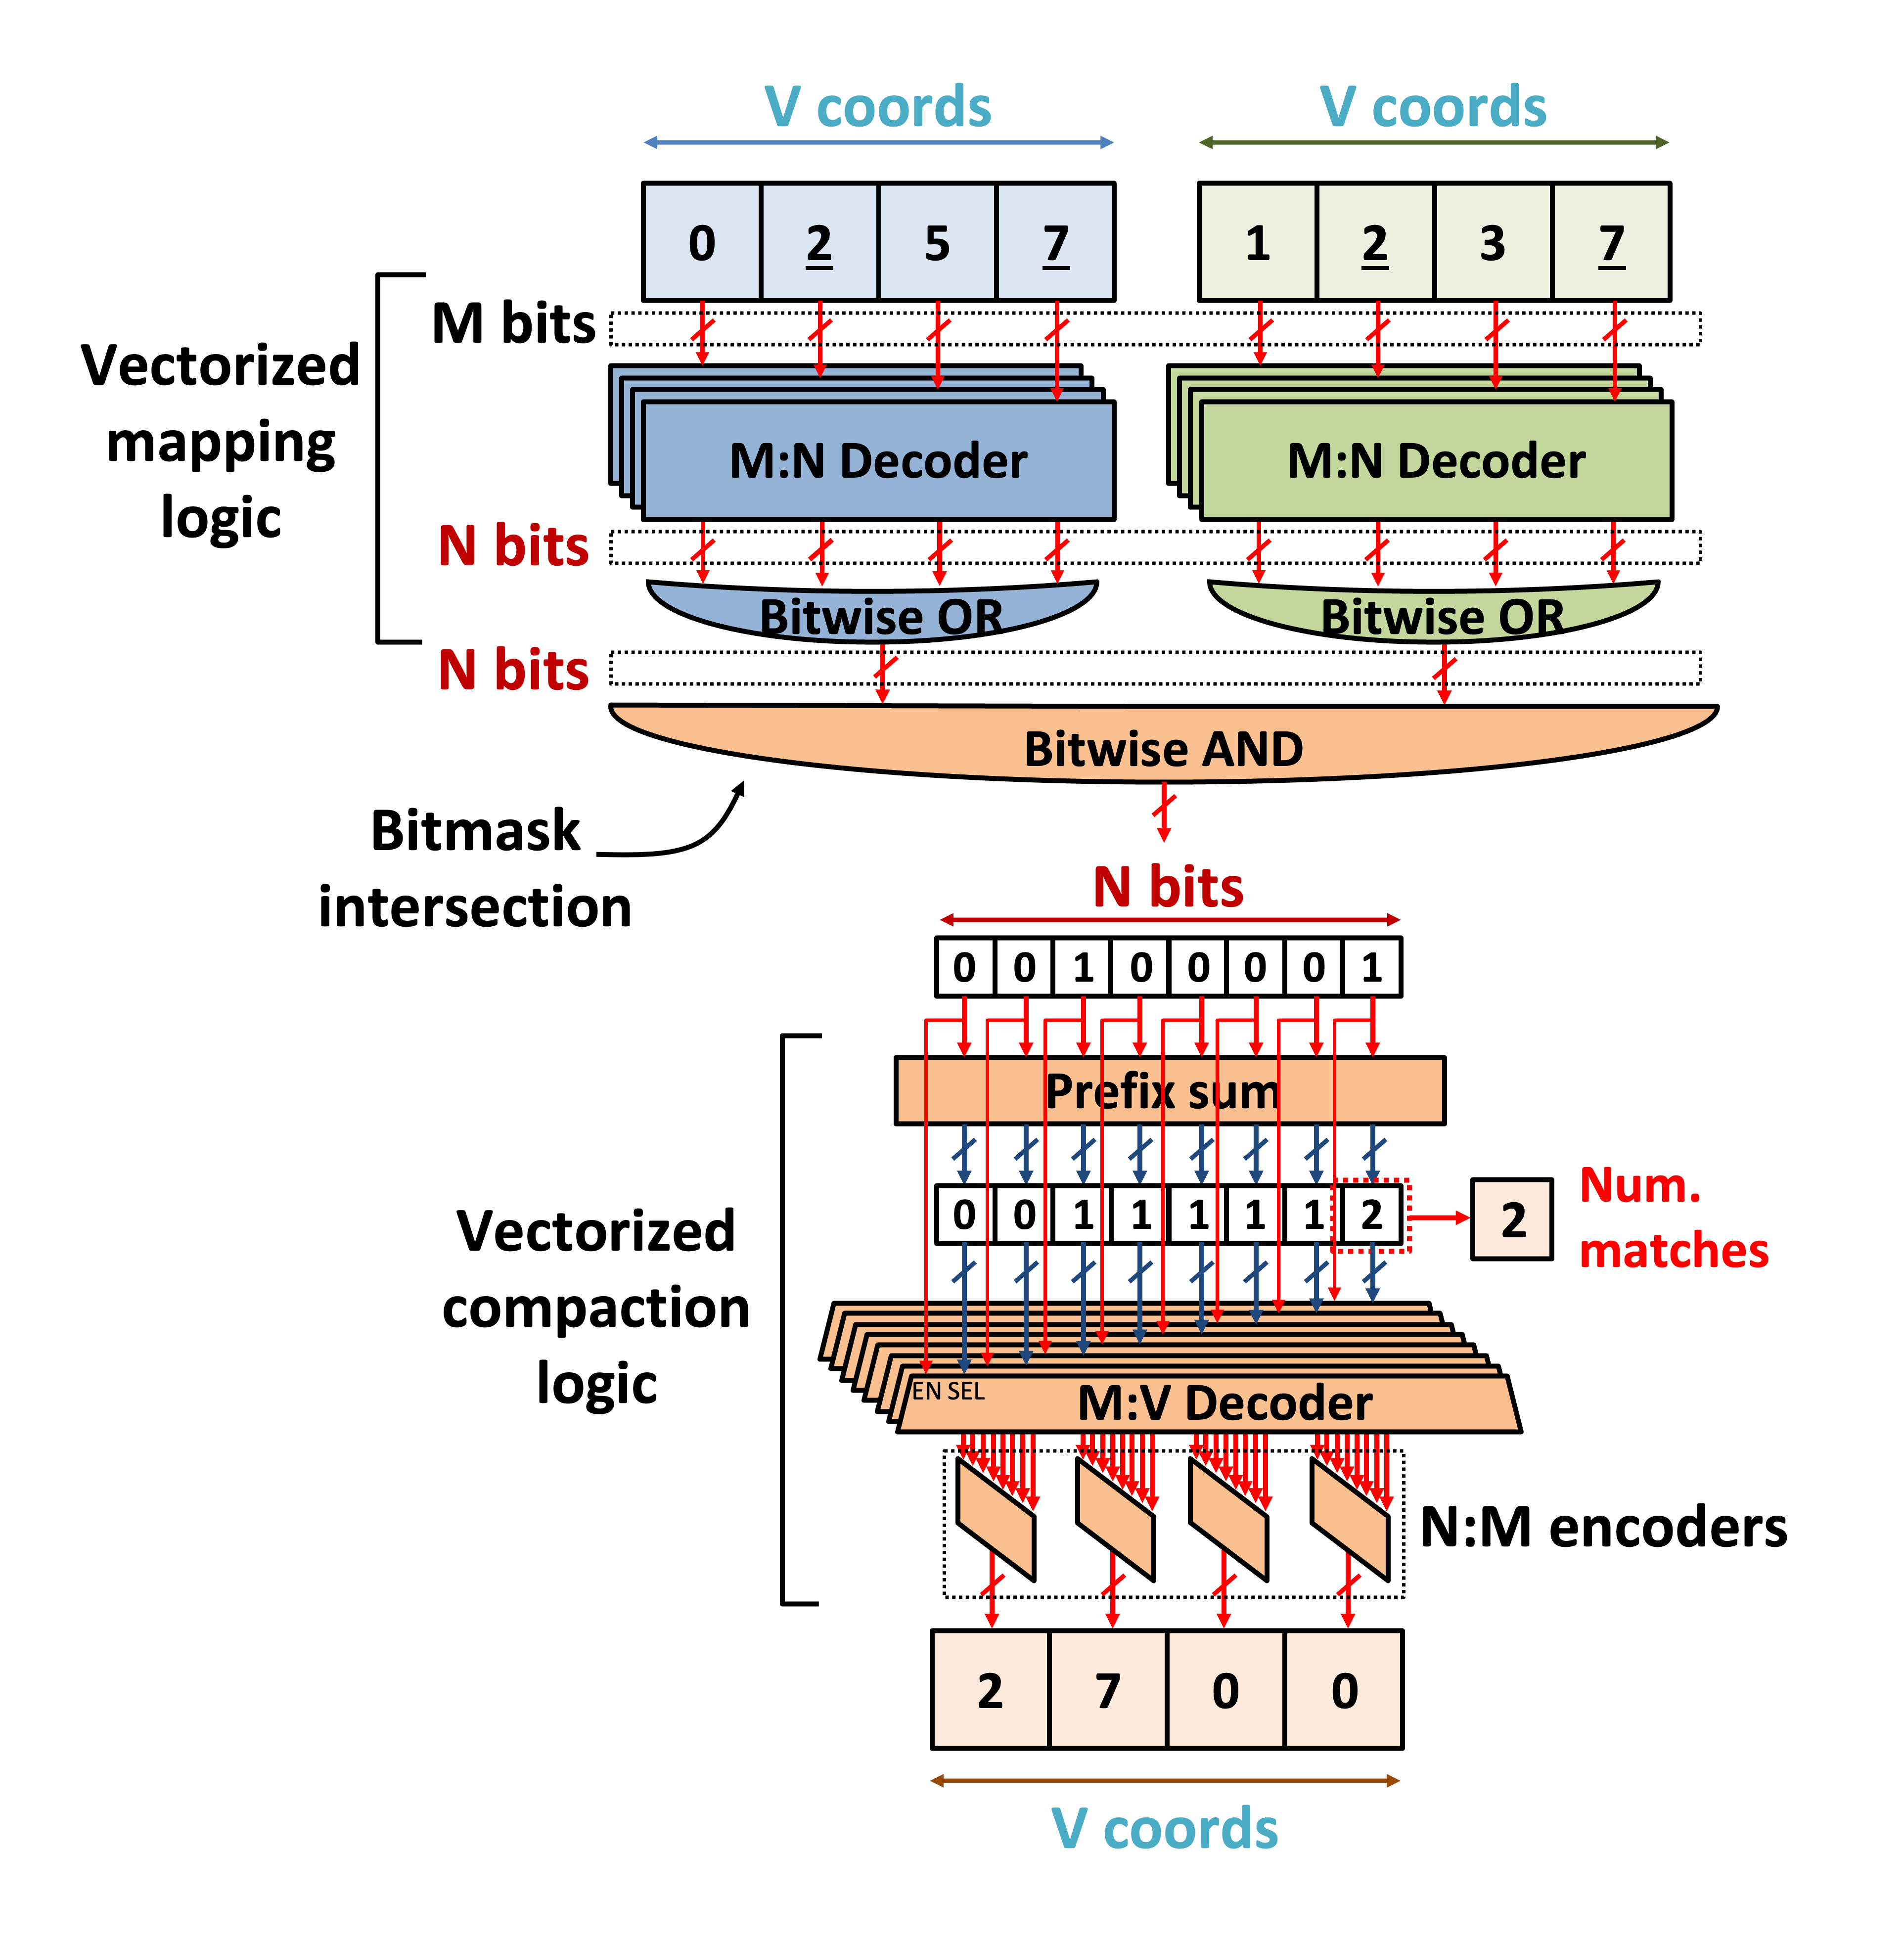
\includegraphics[width=0.95\textwidth]{figures/direct_mapped_isect.png}
    \caption{Vectorized direct-mapped intersection unit. Consumes two coordinate metadata vectors, and outputs a compacted and sorted vector of common elements, along with a count of common elements ($num\_matches$.) Output vector indices greater than $num\_matches - 1$ have undefined values.}
    \label{fig:direct_mapped_isect}
\end{figure}

\clearpage

The implementation, shown in Figure~\ref{fig:direct_mapped_isect}, is based on a ``direct-mapped approach'', analogous to direct-mapped cache. An array of decoders maps the input vector operands from position-space into coordinate-space; this mapping is performed in parallel. This yields two bitmasks (one per operand); in a given operand's bitmask, the index of each hot bit corresponds to an explicit coordinate value in the corresponding input vector. A bitmask intersection is then performed, yielding a new bit-vector in which each hot bit corresponds to a \textit{common} explicit coordinate value between the two vectors. Compaction logic maps these common coordinates back into position-space, yielding a sorted vector of explicit coordinate values which are common to both input vectors.

\textbf{Vectorized parallel direct-mapped intersection unit parameters:}

\begin{itemize}
    \item Vector size (applies to input and output.)
    \item Fiber size (the coordinate-space length of the two sparse fibers being intersected.) This determines the size of the bitmasks.
    \item Coordinate metadata bitwidth, i.e. the number of bits per element in the input and output vectors.
\end{itemize}

For example, a fiber spanning the range of coordinate values $[0,L-1]$ would require the fiber size parameter to be set to L, regardless of the number of non-zero values in the fiber.



\subsubsection{Parallel bitmask intersection unit (SparTen\cite{sparten}-like)}

The parallel bitmask intersection unit is modeled after the bitmask intersection unit from SparTen\cite{sparten}. It operates exclusively on bitmask inputs, and finds all matches within a single cycle. It does not require vector pipelining or combinational unrolling.

\textbf{Vectorized parallel bitmask intersection unit parameters:}

\begin{itemize}
    \item Number of input bits
\end{itemize}

The parallel bitmask intersection unit applies a straightforward bitwise-AND operation and outputs the result.

% Bitmask intersection
\begin{figure}[H]
    \centering
    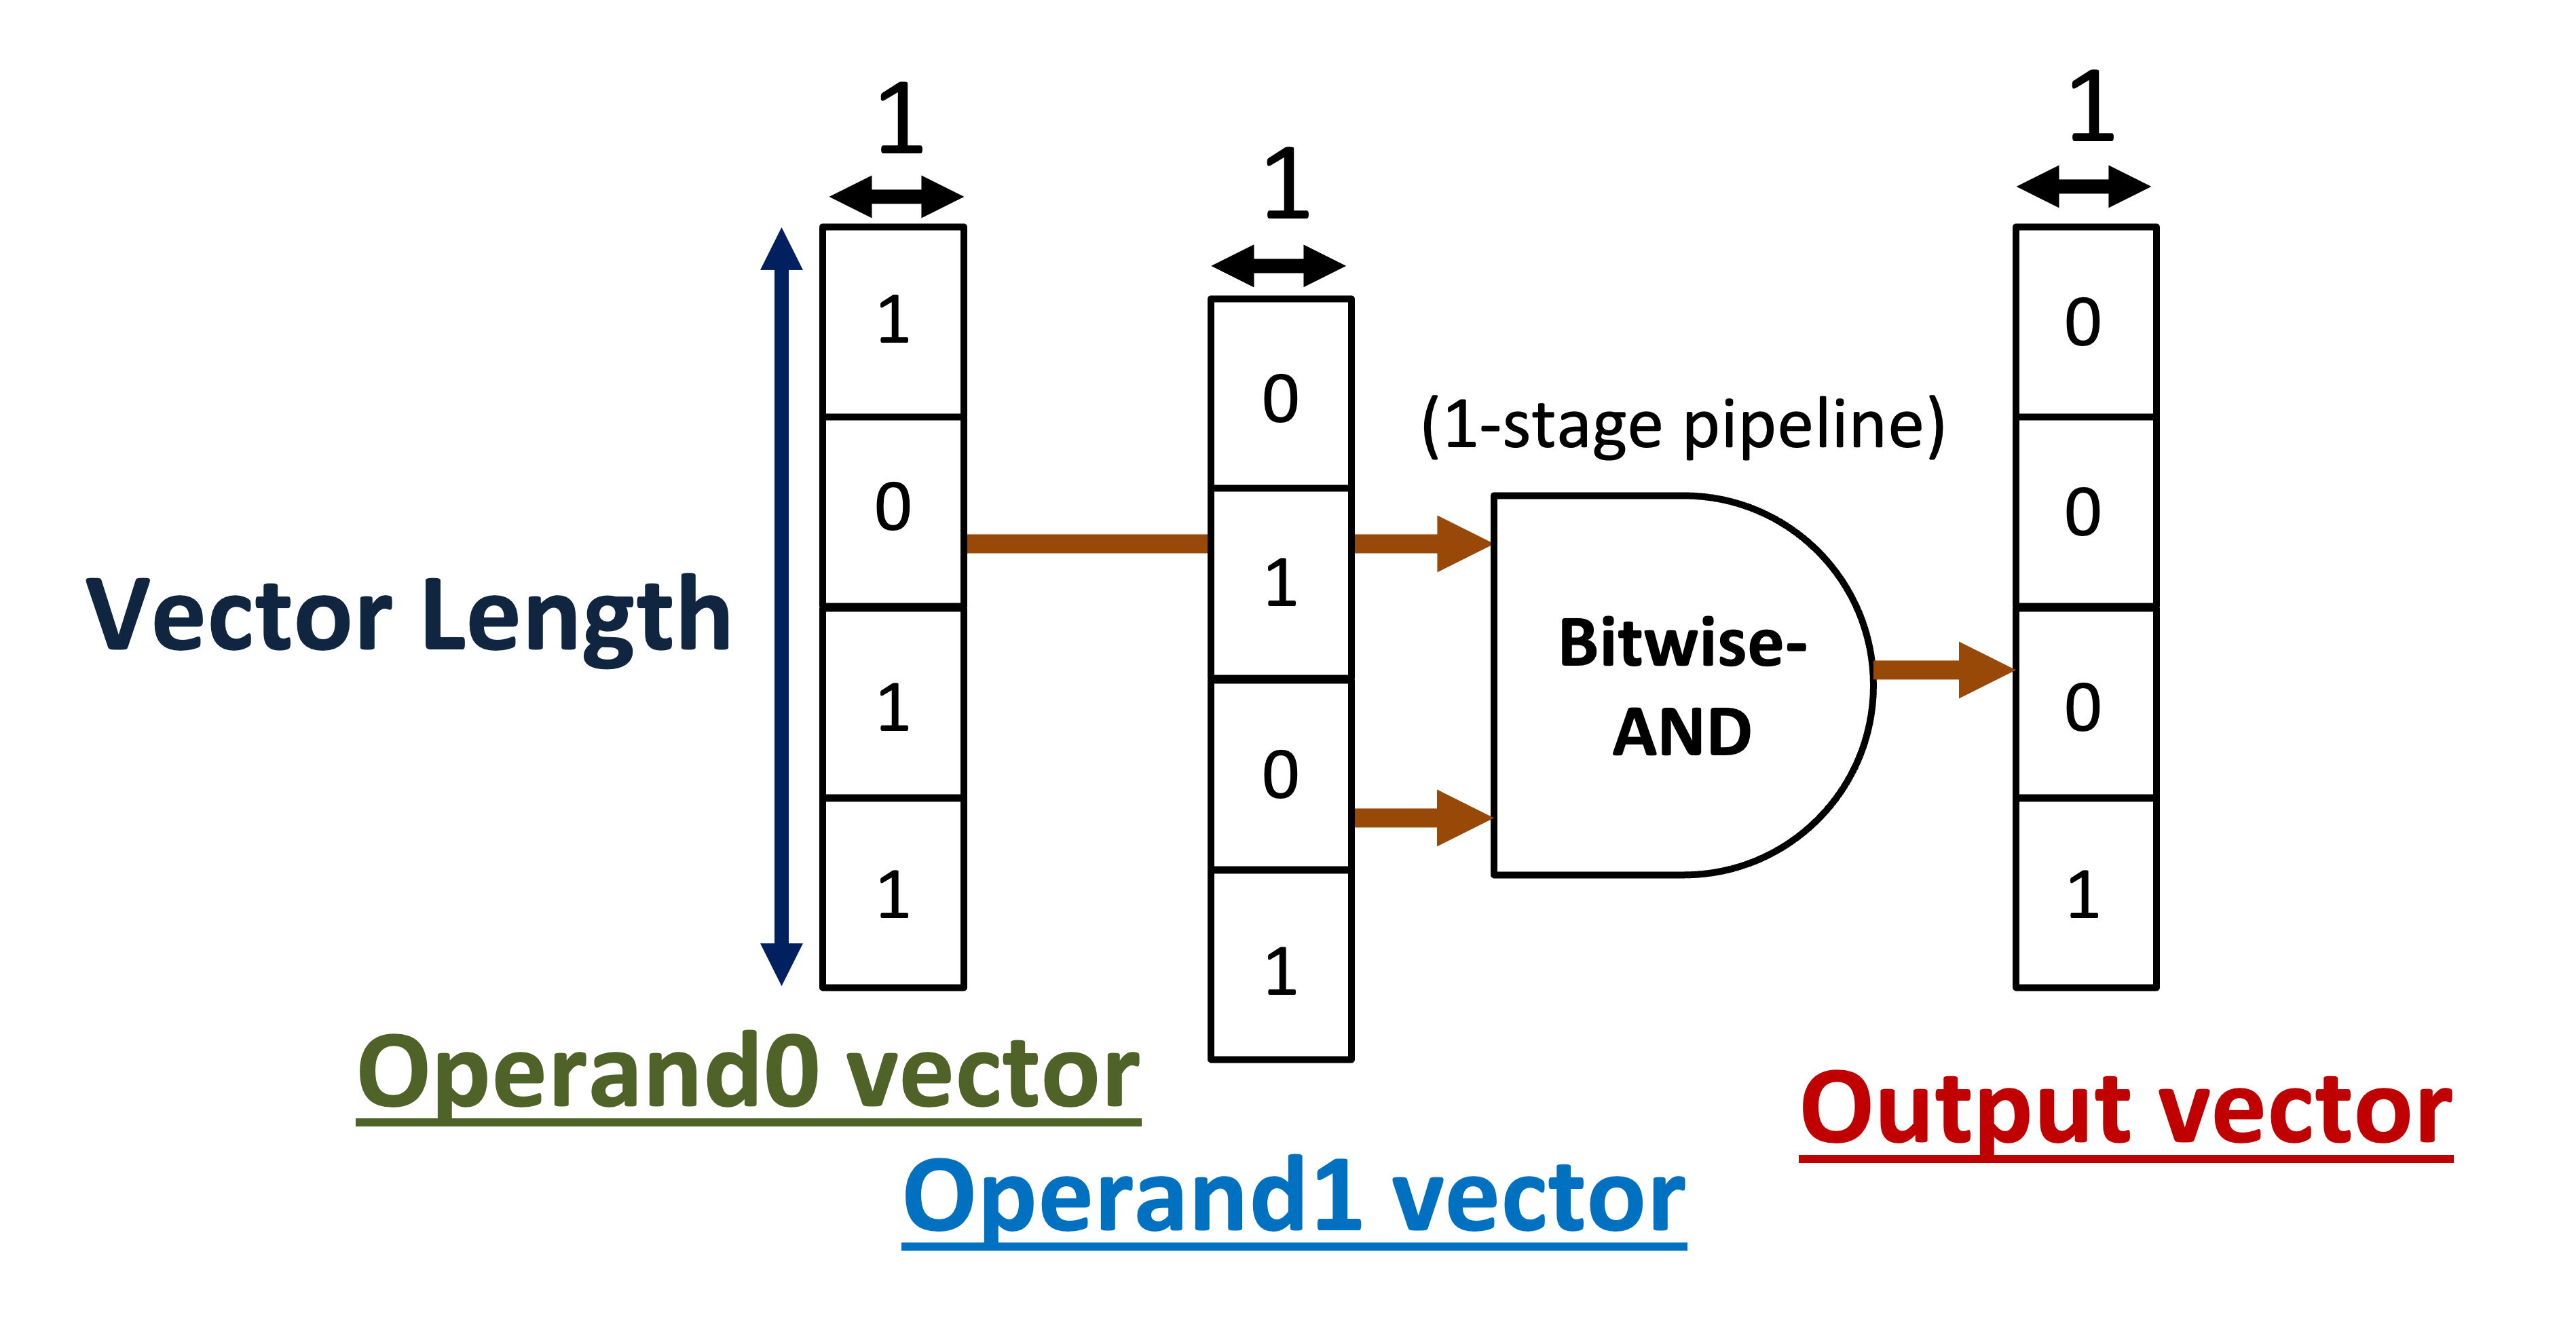
\includegraphics[width=\linewidth]{figures/bitmask_intersection.png}
    \caption{Bitmask intersection vector pipeline.}
    \label{fig:bitmask_intersection}
\end{figure}
\chapter{Modeling techniques for SAF microarchitectures}
\label{chapter:modeling}

Recall that assigning analytical models to SAF microarchitecture primitives is important in order to enable evaluation and comparison of designs. This section will introduce the overarching modeling strategy employed in this work, tying together energy, area and workload modeling into a single scheme. The following considerations are relevant:

\begin{itemize}
    \item Recall from Chapter~\ref{chapter:conceptual_framework} that one of the goals of this work is to associate SAF microarchitecture primitives with analytical cost models (i.e. models of energy and area.) Toward that end, Chapter~\ref{chapter:rtl} introduced a number of RTL designs which were developed and characterized for this work.
    \item However, we still need a way to convert RTL characterization results, into SAF microarchitecture primitive models with well-defined energy-per-action and area.
    \item Also recall from Chapter~\ref{chapter:conceptual_framework} that another goal of this work is to decouple SAF microarchitecture from architecture and dataflow. As shown in Figure~\ref{fig:sparse_sbuff_wkld_overview}, we hope to encapsulate all details of architecture and dataflow behind format interfaces with well-defined measures of workload.
\end{itemize}

Recall that the RTL in Chapter~\ref{chapter:rtl} is parameterized. The power-consumption and area of RTL components will scale with the parameter values. However, more subtly, the \textit{load-handling capability} of the RTL components also scales with the parameter values. For example, a naive two-finger-merge-based intersection unit will be able to intersect more input operands per cycle, if it is constructed with a greater degree of input vectorization; or, a prefix sum unit designed for operands which have some number of bits, will be able to support operands with a larger range of possible values if the number of bits is increased. Thus RTL parameters represent a tradeoff between cost (power, area) and load-handling capability.

The motivation for assigning a measure of workload to each format interface at the outset, is so that the scale parameters of the SAF microarchitecture may be tuned properly. The SAF microarchitecture scale parameters should be set such that

\begin{itemize}
    \item The SAF microarchitecture can process sparse format metadata at the rate which it is being served over the format interface by the smartbuffer.
    \item The SAF microarchitecture is capable of serving processed outputs back to the buffer via the format interface, at the rate which the buffer was designed for.
\end{itemize}

Failure to meet either of the above requirements should in principle lead to a slowdown in the whole design.

\section{Load modeling}

This section describes a multi-dimensional measure of the load that architectural buffers and arithmetic units impose on SAF microarchitectures. The area and action-energy of each SAF microarchitecture will scale as a function of load-handling requirements; having a way to quantify loading will allow us to solve for RTL parameters that minimize cost while meeting load handling requirements.

On first blush, it might seem appropriate to use a single scalar quantity to characterize both load and load-handling capability of a component. For example, the \textit{throughput} (number of inputs processed per time) would seem like a good candidate for measuring load and load-handling requirements (since FLOPs is a common compute performance metric.)

However, it quickly becomes apparent that load and load-handling ability are multi-dimensional; what follows is a list of factors which influence loading and load-handling requirements:

\begin{itemize}
    \item \textbf{Word-width.} A microarchitecture capable of handling the throughput imposed by some workload, may nonetheless be unsuitable if i.e. the microarchitecture is expected to process sparse format metadata possessing a greater bitwidth than what the microarchitecture was designed for. Thus, word-width is a dimension of load, and the upper limit on word-width is a dimension of load-handling capability for a particular component.
    \item \textbf{Size of abstract dense rank which underlies a sparse fiber.} Consider a bitmask intersection unit, as employed in the SparTen accelerator paper \cite{sparten}. The degree of parallelism of the bitmask intersection unit microarchitecture is not a function of the throughput of metadata nor of the number of bits in a metadata word (which is in fact equal to one for bitmask format), but rather the parallelism must meet or exceed the cardinality of the abstract dense ranks which underly the sparse fibers being intersected. Thus, the cardinality of the dense rank which underlies a sparse fiber is a dimension of the load on the microarchitecture. The parallelism of the bitmask intersection unit exemplifies a dimension of the microarchitecture's load-handling capability, specifically an upper-limit on dense rank cardinality which the microarchitecture can handle.
    \item \textbf{Memory access width.} The SAF microarchitecture must be able to receive sparse format metadata in chunks equal to the memory's access bitwidth - i.e., for metadata with a bitwidth of 4 stored in a memory with 8-bit-wide reads, up to two metadata words may be made available to the SAF microarchitecture per access, worst-case. If the SAF microarchitecture only needs to read format metadata a few times over many cycles, then the latency of sequentially processing multiple metadata words can be hidden inside the time between wide reads. However, a SAF microarchitecture that is making wide memory accesses every cycle cannot hide the latency of sequential processing and thus requires a (probably more costly) SIMD design. This motivates memory access width as a dimension of load and load-handling capability.
    \item \textbf{Local architectural throughput.} Suppose that an architecture uses a SIMD MAC unit capable of 4x $C = C + A \times B$ operations per cycle to compute an inner-product; let's define $4$ MACs/cycle as the \textit{arithmetic throughput requirement.} To avoid MAC underutilization, the arithmetic throughput requirement in turn poses requirements on the whole design; for example, four $A$ and four $B$ operands per cycle are read from the $A$ and $B$ buffers respectively. 

    % Radix-2 intersection example figure
    \begin{figure}[H]
        \centering
        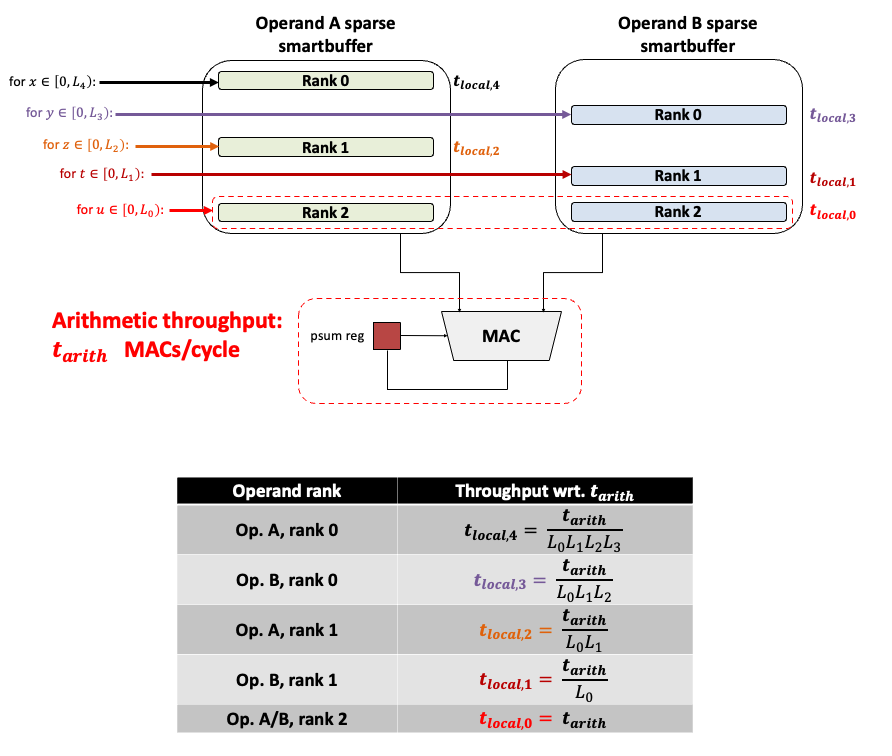
\includegraphics[width=\linewidth]{figures/local_throughput_diagram.png}
        \caption{The local throughput at each rank grows with increasing arithmetic throughput, and shrinks in proportion to the stride of the loop(s) which the fiber is bound to.}
        \label{fig:local_throughput_diagram}
    \end{figure}

    As an optimization, the designer implements a bidirectional skipping SAF between buffers $A$ and $B$. The skipping microarchitecture intersects $A$ and $B$ metadata and outputs a pair of $A$ and $B$ data read addresses for each intersection match. Consider what load-handling requirements the skipping microarchitecture must be designed for, in order to avoid MAC under-utilization: the skipping microarchitecture must serve $4$ $A$ addresses and $4$ $B$ addresses per cycle in order to facilitate reading 4 data values per cycle from each operand. Notably, this is a requirement on the skipping microarchitecture which results directly from the arithmetic throughput design-point.

    Note that in the above example, the skipping microarchitecture, buffers, and MAC are all synchronized with the innermost loop of the mapping loop-nest; this is the fastest loop. Conversely, the outermost loops of the mapping loop-nest have greater latency between loop iterations (i.e. more cycles-per-iteration). Microarchitectures synced to slower loops can maximally exploit latency-hiding to relax throughput-handling requirements by spreading out sequential processing over the time between loop iterations. Microarchitectures synced to faster loops must be capable of handling higher processing throughput without exploiting latency hiding. This state of affairs is summarized in Figure~\ref{fig:local_throughput_diagram}
    
    As a precedent, Sparseloop\cite{sparseloop} assumes that data is pre-tiled to match the loop-nest. Under this assumption there is a reasonably clean mapping from loops in the loop nest to fibers in the fibertree of an operand, and thus a microarchitecture which interacts with fiber $i$ must support the throughput imposed by the corresponding loop in the loop-nest. For example, the inner-most loop must keep pace with the arithmetic throughput-handling requirement imposed by the MAC, so any microarchitecture which interacts with the fiber(s) corresponding to the inner loop must also keep pace with the arithmetic throughput requirement. \textit{All other things being equal}, the microarchitectural throughput-handling requirement decreases monotonically as you ascend hierarchically within a fibertree, because successively higher fibers correspond to successively slower loops. 
    
    Define \textit{local architectural throughput} as the unique throughput requirement for processing a \textit{particular} fiber within a \textit{particular} buffer, owing to the synchronization of the whole architecture with the mapping loop nest. Local architecture throughput is a key dimension of the load which the architecture imposes on a SAF microarchitecture. Consequently, throughput-handling capability is a key design requirement - \textit{but not the only key requirement} - for the SAF microarchitecture.

    We can shorten local architectural throughput to ``local throughput'' or $t_{local}$.
    
    \item \textbf{Degree of fiber sparsity.} Suppose that a fiber with a bitmask representation format resides in some buffer within an architecture. The local architecture throughput requirement for processing this fiber places a lower bound on how many non-zero fiber payloads must be traversed per cycle.

    Since it is given that the fiber is subject to a bitmask format SAF optimization, a format microarchitecture is required for parsing the metadata format. Based on the programming model developed in this work, the buffer will have several format interface ports to facilitate fiber metadata processing: \textit{md\_out}, \textit{pos\_in}, \textit{at\_bound\_in}. The format microarchitecture's ports are wired to read bitmask metadata from the buffer \textit{md\_out} port, and generate an active-high signal at \textit{at\_bound\_in} to signal when the entire fiber has been processed.

    How do we derive the format microarchitecture throughput-handling requirement from the local architectural throughput requirement associated with the fiber? The local architectural throughput applies to the rate of traversing non-zero payload values within the fiber, and the number of non-zero payloads may be much less than the dense size of the abstract rank associated with the fiber. In contrast, the number of $1$-bit bitmask metadata words matches the dense rank size regardless of how many non-zero payloads the sparse fiber has. Metadata parsing by the format microarchitecture must keep pace with the traversal of non-zero payloads in the fiber, thus if the fiber is 90\% sparse/10\% dense, $10$ $1$-bit bitmask metadata words must be parsed per non-zero data value on average; if the fiber is 99\% sparse/1\% dense, $100$ $1$-bit bitmask metadata words must be parsed per non-zero data value on average.

    More generally, for a bitmask-formatted fiber with local architectural throughput requirement $t_{local}$ (in payloads/cycle) and a sparsity fraction $s$, the format microarchitecture must support a metadata parsing throughput of

    \[t_{parse} = \frac{1}{1-s}t_{local}\]

    Of course, this relationship only holds for bitmask representation format. A representation format such as coordinate-payload has one explicit-coordinate metadata value per non-zero payload, thus \[t_{parse} = t_{local}\]

    The point is, sparsity $s$ matters because it \textit{sometimes} modulates the microarchitectural throughput-handling requirement imposed by a fiber's local architectural throughput, and thus fiber sparsity is a key dimension of load.
\end{itemize}

\subsection{Workload vectors}
\label{sec:loadspaces}

To concisely and effectively model loading and load-handling capability, this work introduces the concept of \textit{workload vectors} for representing the workload imposed on a SAF microarchitecture. The dimensions of a workload vector are based on the quantities discussed in the previous section, are represented graphically in Figure~\ref{fig:workload_representation}, and are summarized in Table~\ref{table:workload_dimension_mnemonics}.

% Loadspace dimensions
\begin{figure}[H]
    \centering
    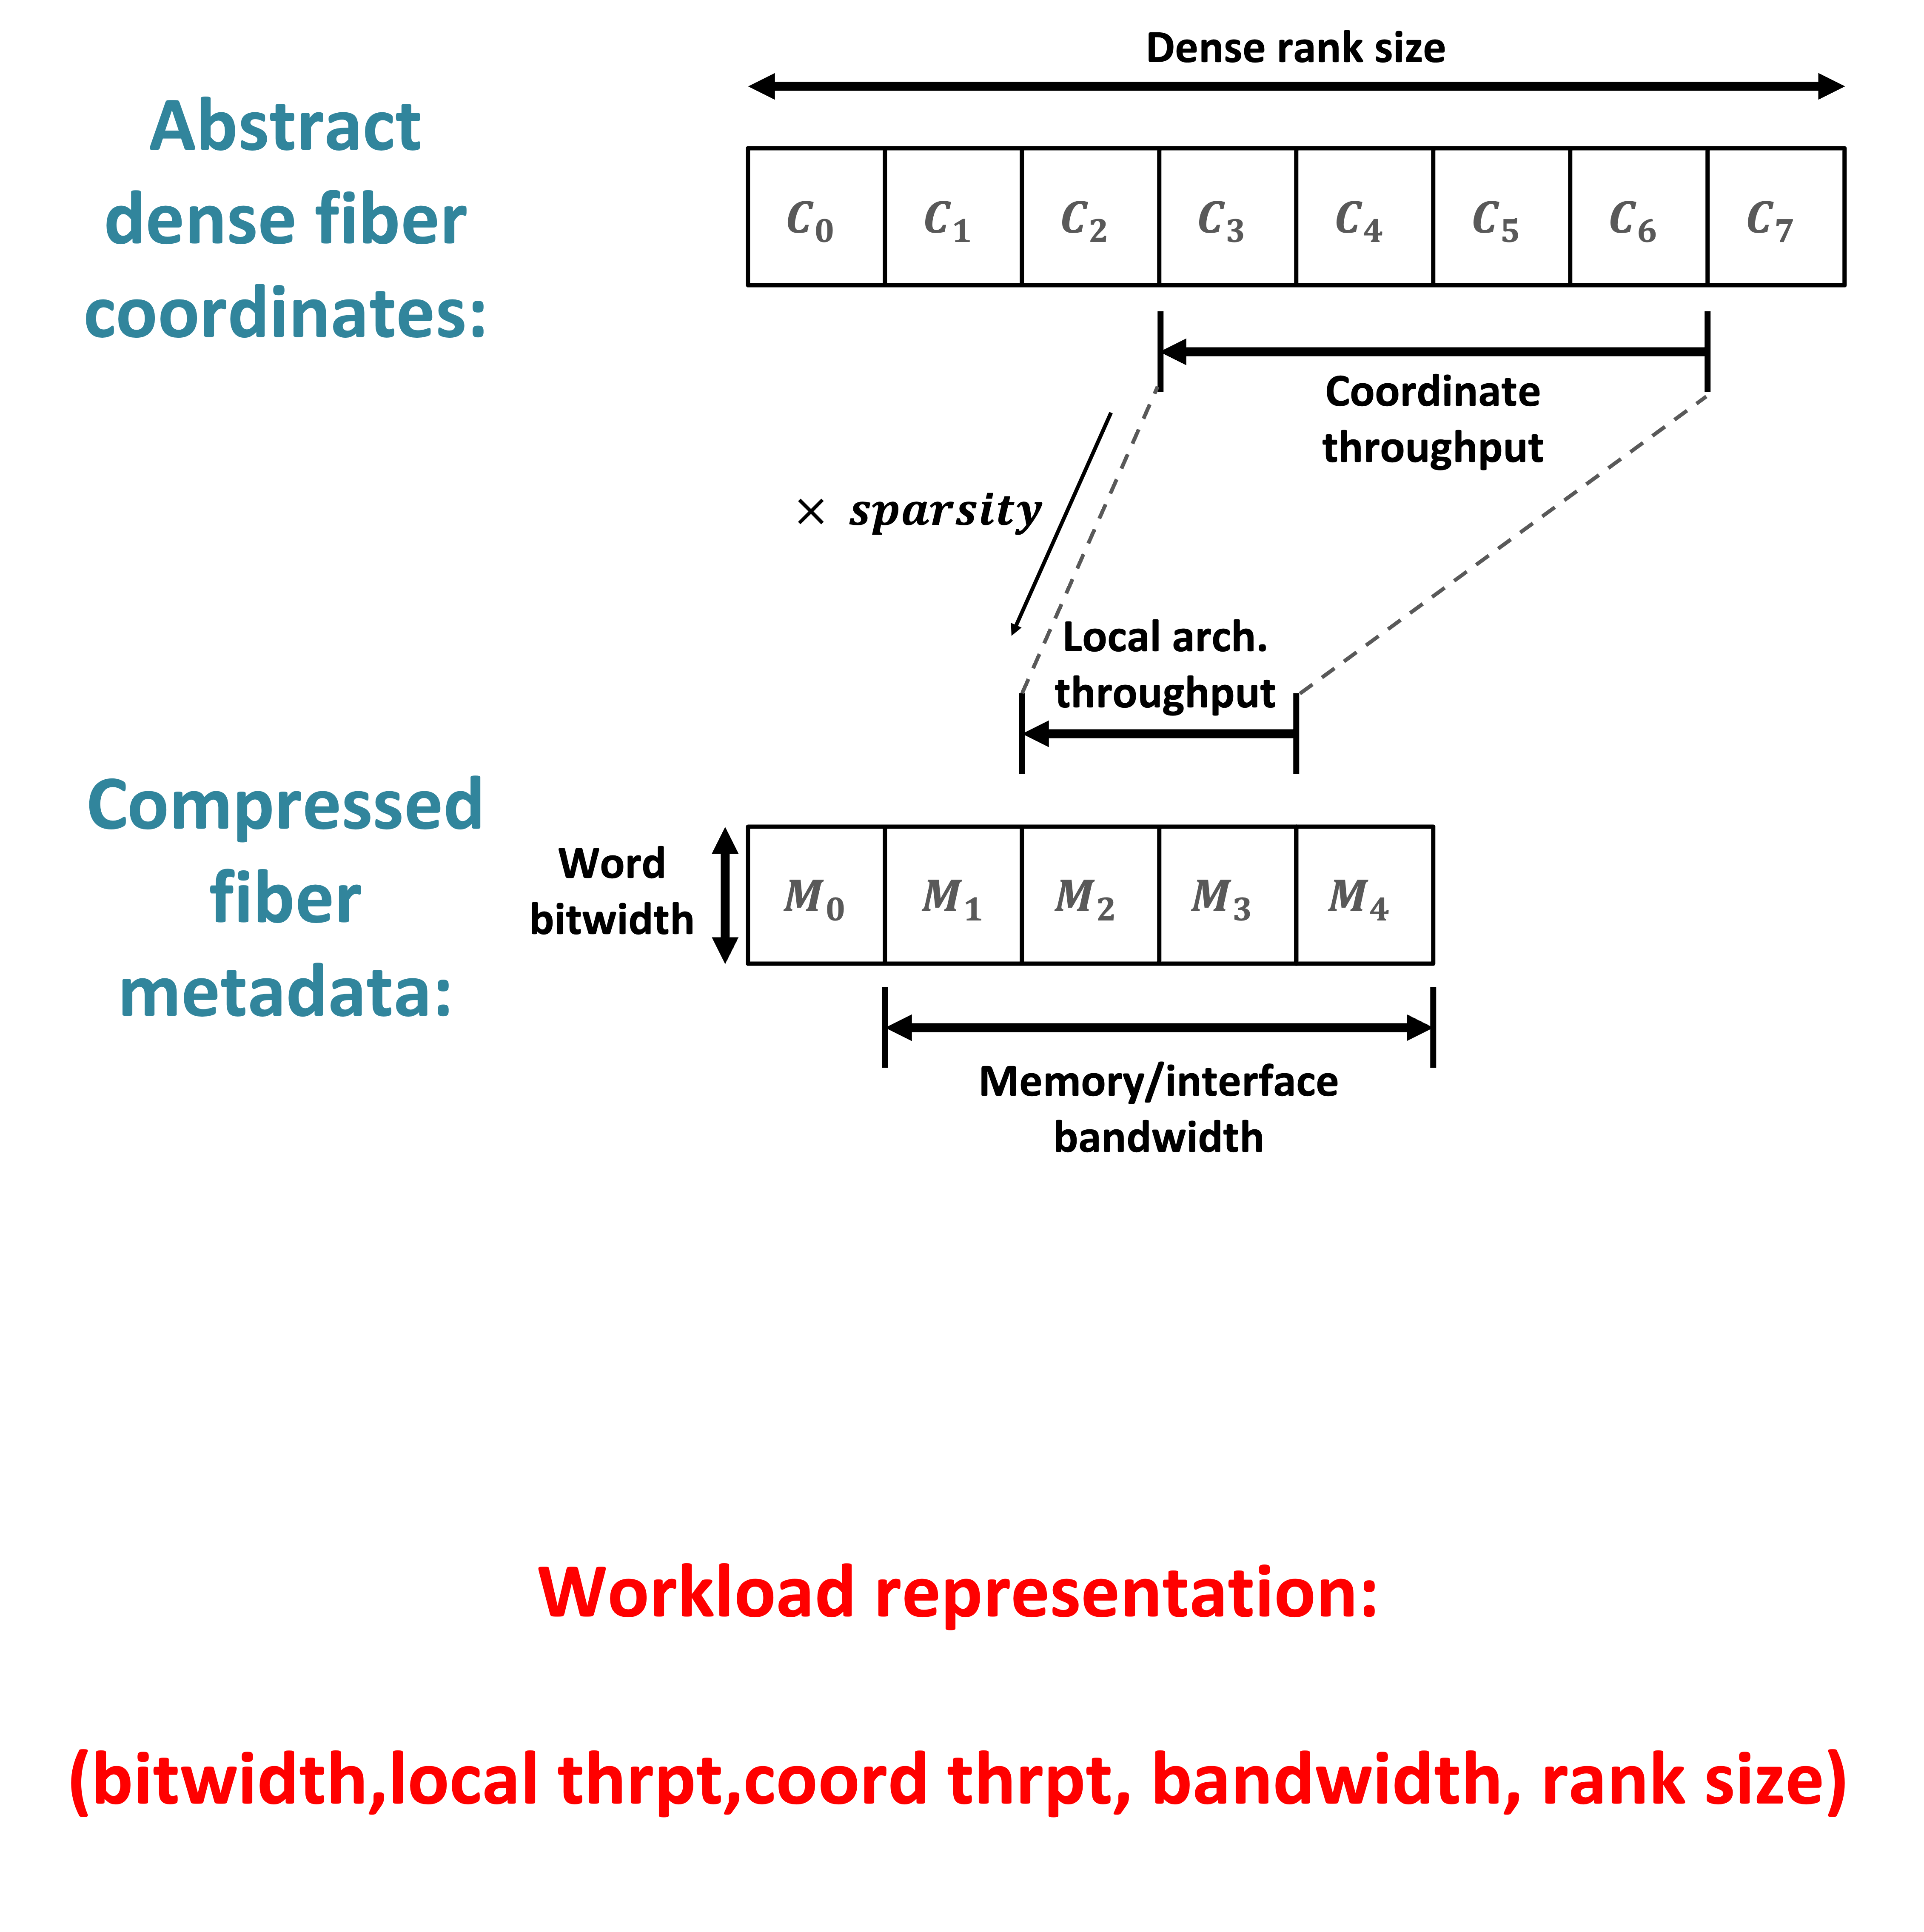
\includegraphics[width=\linewidth]{figures/workload_representation.png}
    \caption{This work proposes modeling workloads as ``workload vectors''. Here, \textit{word bitwidth},  \textit{local architectural throughput}, \textit{coordinate throughput}, and \textit{dense rank size} are proposed as key workload dimensions when designing SAF microarchitectures.}
    \label{fig:workload_representation}
\end{figure}

    \begin{table}[h]
        \centering
        \caption{Mnemonics for workload dimensions.}
        \label{table:workload_dimension_mnemonics}
        \begin{tabular}{||c|c|c|c||}
            \hline \hline
            Workload Dimension & Mnemonic & Stands for & Units \\
            \hline \hline
            Dense rank size & nc & num. coordinates & Coordinates \\
            \hline
            Local throughput & pr & position rate & Words/Cycle \\
            \hline
            Sparsity & sp & sparsity & \% \\
            \hline
            Bitwidth & ww & word width & Bits \\
            \hline
            Bandwidth & bw & read width & Bits \\
            \hline \hline
        \end{tabular}
    \end{table}

\section{Defining workload boundary conditions}

In this work, the approach to decoupling dataflow from SAF microarchitecture is to abstract dataflow behind \textit{workload boundary conditions} associated with each format interface on each sparse smartbuffer.

Recall from Figure~\ref{fig:format_interface} that a format interface is an IO bundle which allows SAF microarchitecture to interface with a tensor rank resident at some sparse smartbuffer. The wires within the format interface IO bundle (from the smartbuffer perspective) are

\begin{itemize}
    \item pos\_in - input which receives position offsets for looking up payloads.
    \item md\_out - fiber sparse format metadata output.
    \item at\_bound\_in - flag input for resetting traversal.
\end{itemize}

Suppose that the a particular format interface on some smartbuffer, is associated with a particular fibertree rank with dense rank size $nc$, sparsity $sp$, metadata word bitwidth $ww_{md}$, and position word bitwidth $ww_{pos}$. Suppose that owing to the loop nest, the rank is associated with some local architectural throughput $t_{local}$. Finally, suppose that the smartbuffer with this format interface has a read bandwidth of $rw$ bits. Each wire within the format interface IO bundle is associated with a workload boundary condition, as follows:

\begin{itemize}
    \item \textit{pos\_in:} 
    \begin{itemize}
        \item $pos\_in.pr \geq t_{local}$
        \item $pos\_in.ww = ww_{pos}$
        \item $pos\_in.nc = nc$
        \item $pos\_in.sp = sp$
        \item $pos\_in.rw = rw$
    \end{itemize}

    Notably, the constraint on $pos\_in.pr$ is required in order for the rate of payload lookups to keep pace with the loop nest; otherwise, the architecture might experience a slowdown.
    
    \item \textit{md\_out:} 

    \begin{itemize}
        \item $md\_out.pr \leq md\_out.rw/md\_out.ww$
        \item $md\_out.ww = ww_{md}$
        \item $md\_out.nc = nc$
        \item $md\_out.sp = sp$
        \item $md\_out.rw = rw$
    \end{itemize}

    The constraint of $md\_out.pr$ reflects that the format interface may not output sparse format metadata with a throughput rate exceeding the memory's read bandwidth, in words.

    \item \textit{at\_bound\_in:} 

    \begin{itemize}
        \item $at\_bound\_in.pr \leq md\_out.rw/md\_out.ww$
        \item $at\_bound\_in.ww = ww_{md}$
        \item $at\_bound\_in.nc = nc$
        \item $at\_bound\_in.sp = sp$
        \item $at\_bound\_in.rw = rw$
    \end{itemize}
\end{itemize}

\section{Specifying a SAF microarchitecture primitive model}

The previous section introduced workload vectors to describe loading; this section introduces \textit{scale parameter} vectors to describe a component's \textit{workload handling capability.} By way of introducing this concept, this section overviews the approach to specifying SAF microarchitecture primitive models.

\clearpage

\begin{figure}[H]
    \centering
    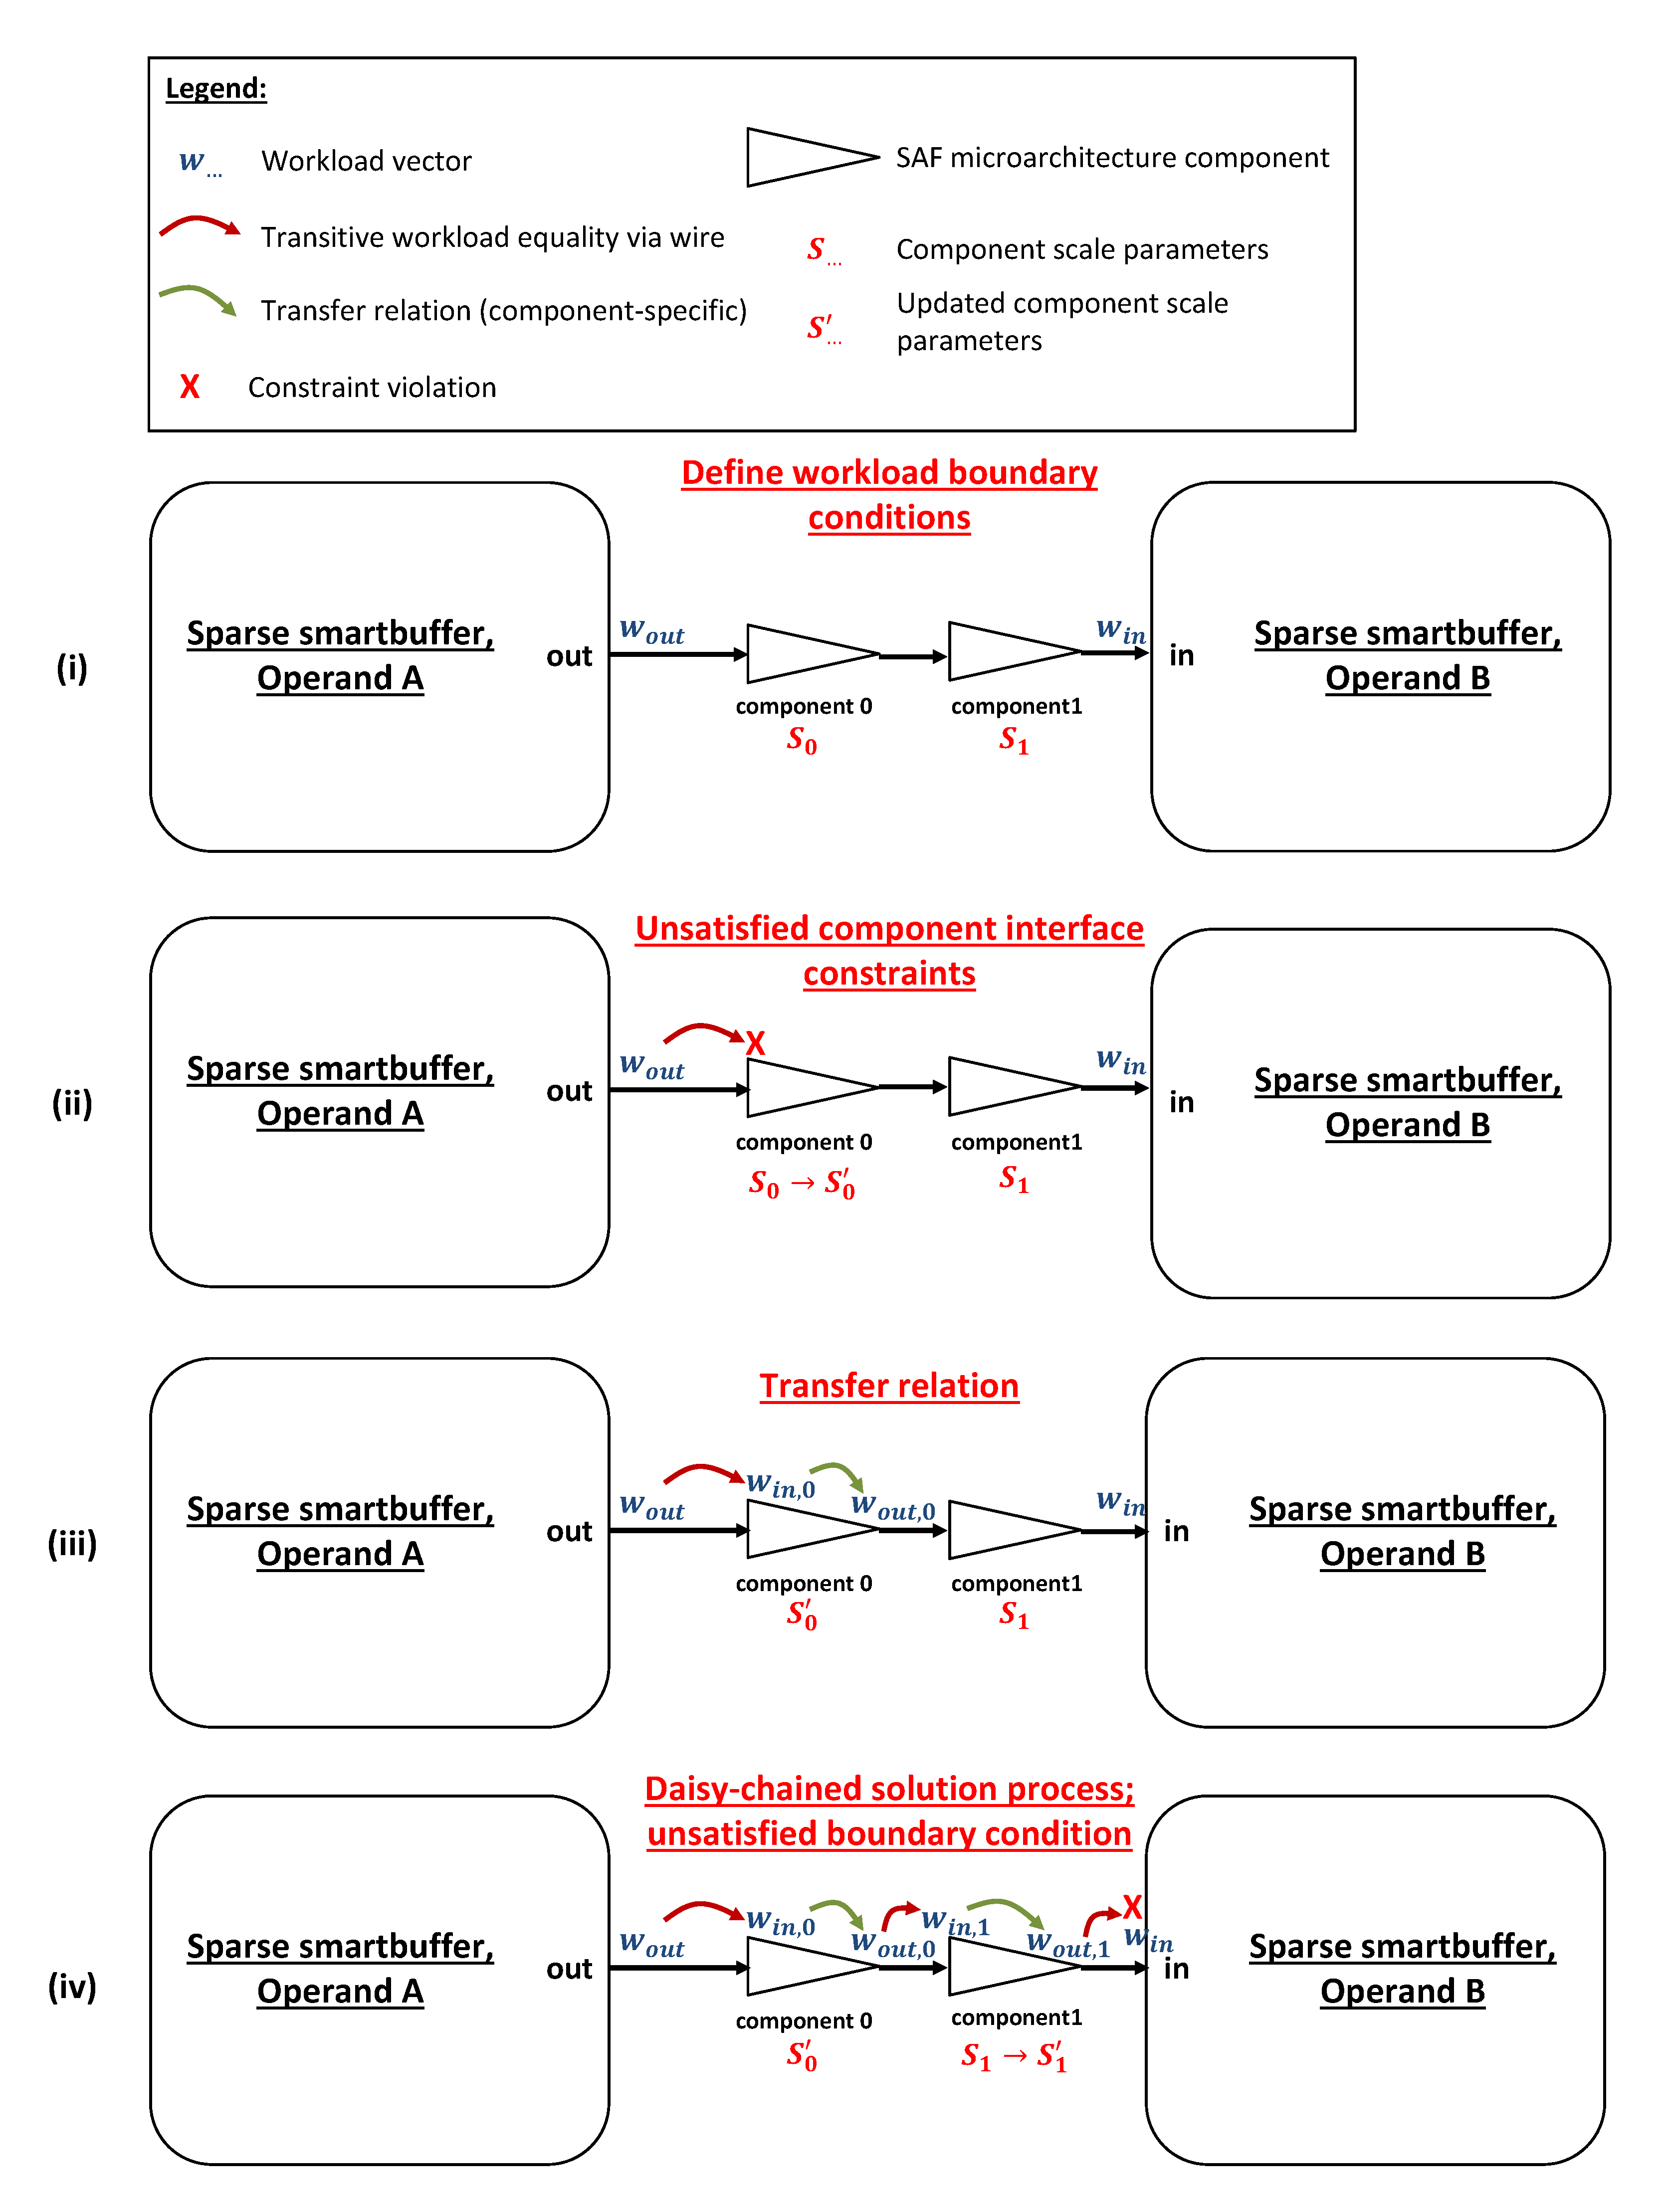
\includegraphics[width=0.8\textwidth]{figures/workload_example.pdf}
    \caption{Example of SAF microarchitecture scale inference, via daisy-chained workload solving.}
    \label{fig:workload_example}
\end{figure}

\clearpage

\begin{figure}[H]
    \centering
    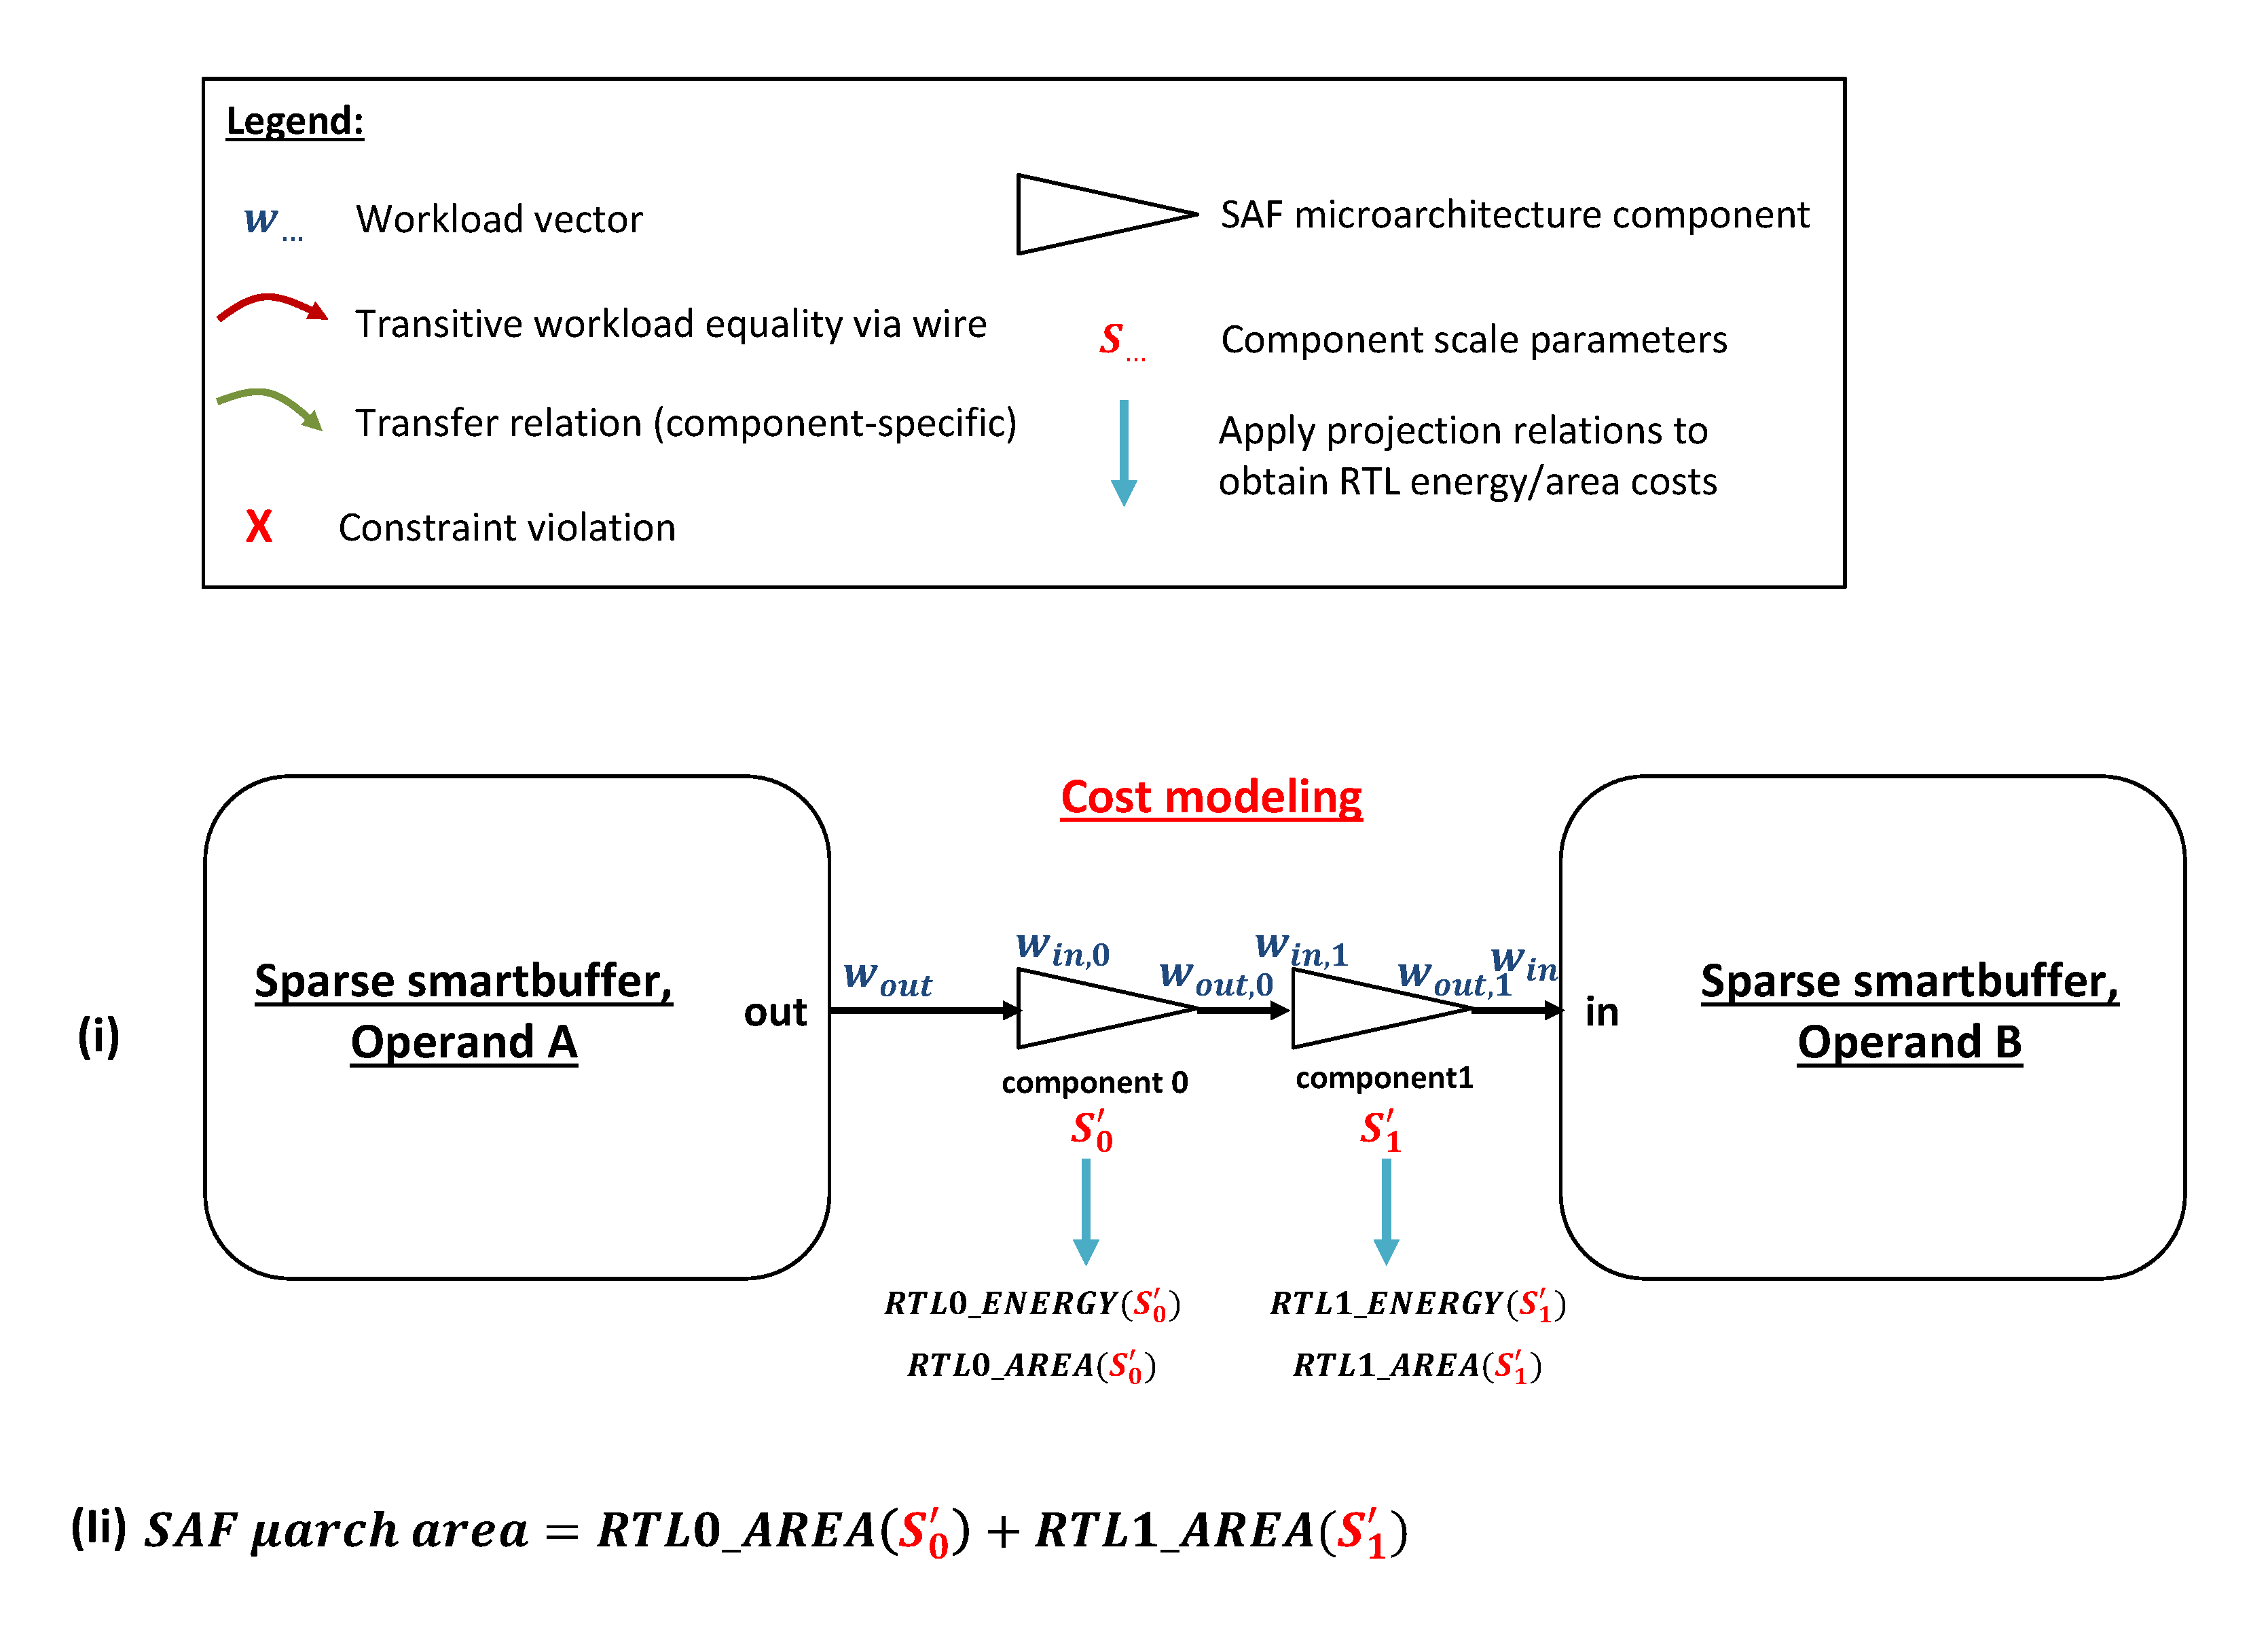
\includegraphics[width=0.8\textwidth]{figures/rtl_objective.pdf}
    \caption{Demonstration of how SAF microarchitecture scale inference makes it possible to derive values for energy and area objective functions.}
    \label{fig:rtl_objective}
\end{figure}

\clearpage

For modeling purposes, a SAF microarchitecture primitive model may be described entirely in terms of:

\begin{itemize}
    \item \textbf{RTL blocks -} A list of RTL modules or ``blocks'' from Chapter~\ref{chapter:rtl} which comprise the component being modeled. Figure~\ref{fig:rtl_objective} reflects that each SAF microarchitecture component may be associated with zero or more characterized RTL components. When the user defines the model of a SAF microarchitecture primitive, they must specify the list of related RTL blocks explicitly.
    \begin{itemize}
        \item \textbf{RTL parameters -} Each RTL block has zero or more parameters which customize the digital logic implementation as a function of the parameter values. RTL parameter values also impact the energy and area cost of a component. The notation for a given RTL parameter is $rtl\_name.param\_name$
        \item \textbf{Example -} A coordinate-payload-format\cite{sparseloop}\cite{szebook} intersection unit\cite{extensor} may (within the context of this work) be constructed out of EXACTLY ONE OF the following RTL blocks defined in Chapter~\ref{chapter:rtl}: a two-fingered intersection unit\cite{extensor}, a skip-ahead intersection unit\cite{extensor}, or a direct-mapped intersection unit.\cite{extensor} (of course the modeling library could be extended to support other options derived from the literature.) The input vectorization parameter of an intersection unit $isect$ would be represented notationally as $isect.md\_in\_vectorization$.
    \end{itemize}
    \item \textbf{Scale parameters -} A set of parameters which determine the SAF microarchitecture primitive's load-handling capability. Figure~\ref{fig:workload_example} shows that each component is associated with a vector $S_x$ of scale parameter values. \textbf{Critically, scale parameters are distinct from taxonomic attributes} - taxonomic attributes are high-level characteristics which reflect choices about algorithm or scaling behavior; once the taxonomic attributes have been specified, \textit{scale parameters represent the low-level design space for sizing RTL blocks in order to satisfy workloads.}
    \begin{itemize}
        \item \textbf{Notation -} $S_x$ is the vector of scale parameters for component $x$.
        \item \textbf{Example -} The scale parameters of a prefix-sum unit are (1) its \textbf{word bitwidth}, and (2) its \textbf{degree of vectorization}. The prefix-sum unit cannot sum a vector which is larger than its vector scale parameter. It cannot correctly sum a vector with words which have more bits than the prefix-sum unit's word bitwidth scale parameter.
    \end{itemize}
    \item \textbf{The component's \textit{constitutive relations} define a unique set of relationships between the workloads applied at each of the component's interface ports, and the parameters of the component's RTL blocks; the constitutive relations should express an intuition about how the component functions.} Constitutive relations are specified at the time when the user writes a SAFTools model. \textbf{The key constitutive relations are:}
    \begin{itemize}
        \item \textbf{Interface constraints.} The interface constraints set \textbf{upper-bounds} on workload at each component input port (i.e. upper-bounds on each dimension of the workload vector at an input port.) This is reflected by Figure~\ref{fig:workload_example}(ii). These upper-bounds are a function of the scale parameter values $S$.
        \begin{itemize}
            \item \textbf{Notation.} $I[S](w_{port0},w_{port1},...)$ is a set of interface constraints on a set of ports' workloads, parameterized by the scale parameters $S$. Typically, $I[S]()$ imposes \textit{upper-bounds}, and upper-bounds increase as $S$ increases along any dimension. \textbf{Critically, component energy/area cost also increases as $S_{comp}$ increases along any dimension.}
            \item \textbf{Corollary.} If a component has scale parameters $S_{comp}$ and the workload applied at $port0$ violates the constraint(s) $I[S_{comp}](w_{port0})$, one can perform ``design-space exploration'' or ``tuning'' of $S_{comp}$ in order to find the minimum-cost $S^\prime_{comp}$ for which $I[S^\prime_{comp}](w_{port0})$ is satisfied by the workload at port0. This is represented in Figure~\ref{fig:workload_example}(ii), where the scale parameters $S_0$ are adjusted to $S^\prime_0$ such that component 0 will support its input workload.
        \end{itemize}
        \item \textbf{Transfer relations.} The transfer relations are \textbf{equations or upper-bound inequalities on output-port workload(s) as a function of input-port workload(s)}; like interface constraints, transfer relations are parameterized by scale parameters. Figure~\ref{fig:workload_example} (iii) and (iv) show how output workload values (or bounds) are derived from input workloads via transfer relations. Transfer relations capture a key intuition that \textbf{SAF microarchitecture primitives frequently exploit forms of filtering or compaction, operations which yield fewer outputs (or fewer \textit{valid outputs}) than inputs.} Critically, this means that if a smartbuffer's output port applies a workload to component 0's input port, and component 0 in turn applies a load to component 1's input port (as is the case in Figure~\ref{fig:workload_example}), the workload at component 1's input port may not be the same as the workload which the smartbuffer imposes on the input port of component 0. Thus, we need transfer relations in order to know how a much workload one component will impose on others.
        \begin{itemize}
            \item \textbf{Notation.} $T[S_{comp}](w_{port\_in0},w_{port\_in1},...)$
            \item \textbf{Example.} Intersecting two compressed sparse coordinate payload fibers, with $C_0$ and $C_1$ non-zero values respectively, necessarily yields an output stream which will contain $C_{out}$ non-zero matching metadata values, where $C_{out} \leq C_0$ and $C_{out} \leq C_1$. Suppose that we know (for sake of simplicity) that $C_{out} = 0.5 C_0$. Then $T[S_{comp}](w_{port\_in0},w_{port\_in1},...)$ is a set containing two relations:

            \[w_{port\_out,pr} \leq 0.5 w_{port\_in0,pr}\]

            \[w_{port\_out,pr} \leq 0.5 w_{port\_in1,pr}\]

            where $w_{port\_out,pr}$, $w_{port\_in0,pr}$ and $w_{port\_in1,pr}$ represent the \textbf{local throughput dimension (mnemonic ``pr'')} of the $port\_out$, $port\_in0$, and $port\_in1$ interfaces, respectively.
            
            \item \textbf{Example.} If two compressed sparse fibers are being intersected, the underlying dense ranks for both fibers necessarily have the same size - and furthermore, the intersected metadata stream at the intersection unit output necessarily also maps back onto the same underlying dense rank. Thus for an intersection unit, the following transfer relations also apply:

            \[w_{port\_out,nc} = w_{port\_in0,nc}\]

            \[w_{port\_out,nc} = w_{port\_in1,nc}\]

            where the $nc$ subscript refers to the dense rank size dimension (mnemonic ``nc'') of each port's workload.
        \end{itemize}
        \item \textbf{Projection relations.} The projection relations allow a SAF microarchitecture primitive's scale parameters to be converted into an analytical model, by adjusting the underlying RTL parameters to match. Projection relations are equations relating RTL parameters to SAF microarchitecture primitive scale parameters.
        \begin{itemize}
            \item \textbf{Notation.} $P[S_{comp}](RTL0,RTL1,...)$
            \item \textbf{Example.} Consider a hypothetical SAF microarchitecture primitive \textit{comp} with with some scale parameter $s \in S_{comp}$, which derives its analytical model from an RTL block \textit{RTL} with a single parameter $p$. Then the projection relations $P[S_{comp}]$ might include

            \[comp.s = RTL.p\]
        \end{itemize}
    \end{itemize}
\end{itemize}

\subsection{Primitive scale inference: solving for scale parameters which satisfy workloads.}

Figure~\ref{fig:workload_example} and Figure~\ref{fig:rtl_objective} summarize the process of \textit{scale inference}, whereby we solve for each SAF microarchitecture primitive's scale parameters $S_x$ where $\{x\}$ is the set of SAF microarchitecture primitive IDs. 

The criteria for valid scale parameters is

\begin{itemize}
    \item All SAF microarchitecture \textit{interface constraints} must be satisfied. If a SAF microarchitecture input is connected to an output wire from a format interface IO bundle, the workload boundary condition associated with that format interface must satisfy the SAF microarchitecture input's interface constraint. If the SAF microarchitecture input is connected to another SAF microarchitecture's output port, the other SAF microarchitecture's output workload must satisfy the SAF microarchitecture input's interface constraint.
    \item For format interface input wires, all \textit{workload boundary conditions} must be satisfied by the SAF microarchitecture output wire connected to the format interface input wire.
\end{itemize}

Scale inference is then a search process over $\{S_x\}$ in order to satisfy the above constraints. Note the following:

\begin{itemize}
    \item SAF microarchitecture primitive interface constraints $I$ and SAF microarchitecture primitive transfer relations $T$ are parameterized by the scale parameters $\{S_x\}$. Thus, adjusting $\{S_x\}$ can (1) make $I$ easier to satisfy by raising upper bounds on workload, or (2) transfer less workload to a downstream component, by adjusting the transfer relation $T$.
    \item Workload boundary conditions associated with format interfaces are immutable.
    \item Projection relations are immutable.
\end{itemize}

The starting-point for scale inference is to flatten all SAF microarchitectures in the entire architecture - i.e., get rid of the higher-level abstractions like SKIP and FMT, and express the microarchitecture entirely in terms of SAF microarchitecture primitives. Having done this, we are left with a graph of all SAF microarchitecture primitives in the architecture, and their interconnections. From this we are able to obtain a large set of relations which define the feasible regions of $\{S_x\}$. And from the projection relations, we are able to define an objective function $f(\{S_x\})$ by mapping scale parameters to RTL parameters, and then looking up characterized RTL metrics based on the parameter values.

This yields a mixed-integer non-linear program (MINLP) for minimizing $f(\{S_x\})$ subject to interface constraints and workload boundary conditions on $\{S_x\}$.

\section{Modeling coordinate-payload intersection units}
\label{sec:c_c_isect_modeling}

Up to this point, this section has been very general. Now, we will show an example of finding transfer relations that are applicable to coordinate-payload bidirectional intersection units.

The difficult part of modeling the transfer relation for coordinate payload intersection units, is determining the relationship between input throughput and output throughput.

The scale parameters of the coordinate payload bidirectional intersection unit are

\begin{itemize}
    \item \textbf{Word width -} The metadata word bitwidth.
    \item \textbf{Input vectorization -} The size of the two metadata vectors being intersected.
    \item \textbf{Pipeline depth -} The depth of the intersection unit's vector pipeline.
\end{itemize}

\begin{figure}[ht]
    \centering
    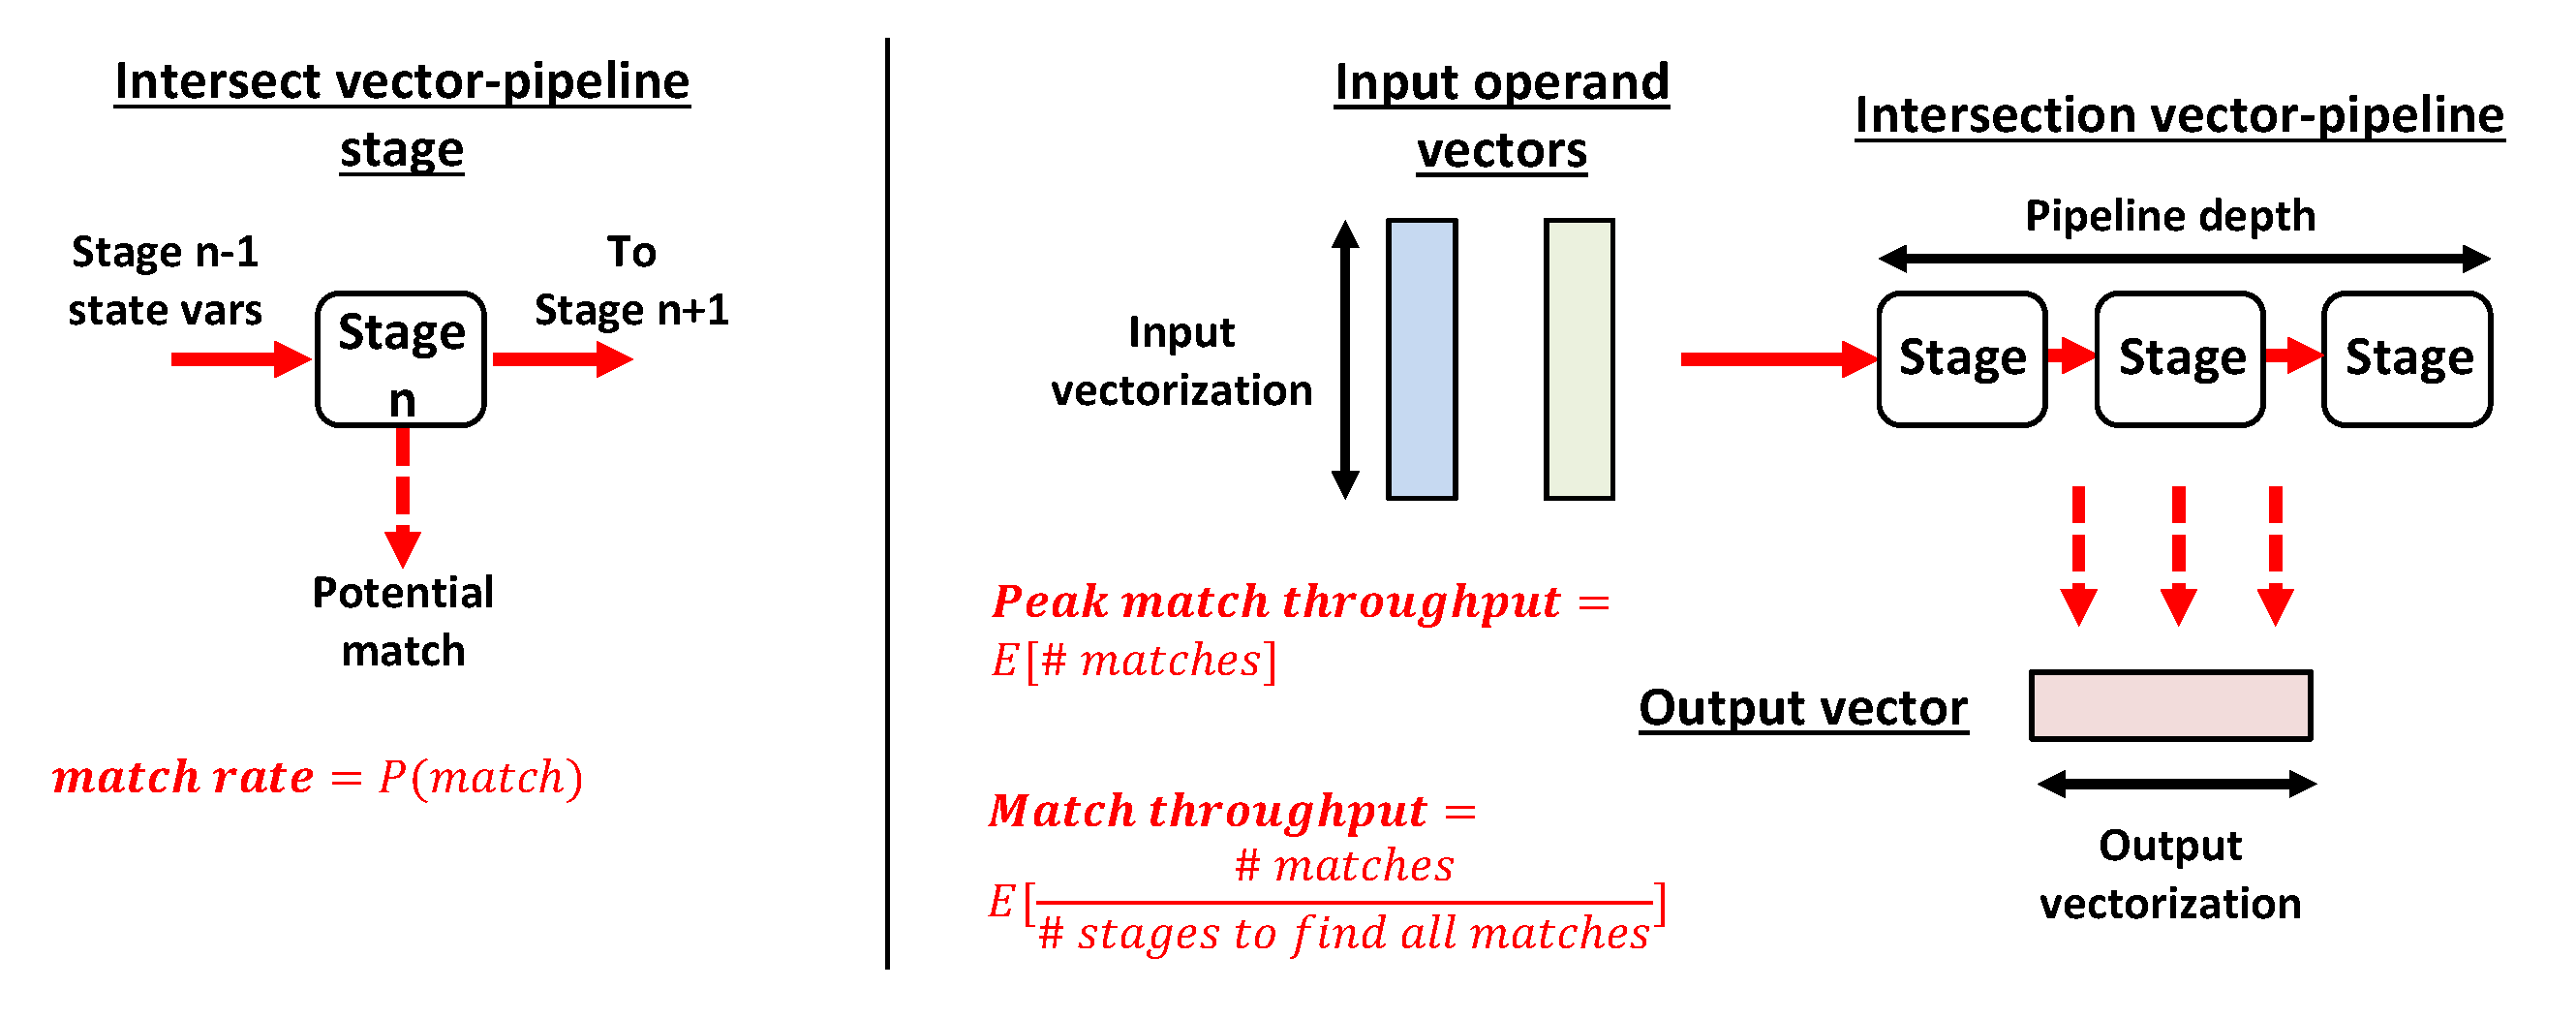
\includegraphics[width=0.95\textwidth]{figures/isect_model.pdf}
    \caption{Diagram of the relationship between the scale parameters of a vector-pipelined intersection unit (vectorization, vector-pipeline depth), and the match throughput.}
    \label{fig:isect_model}
\end{figure}

Figure~\ref{fig:isect_model} summarizes how intersection units are modeled in this work: on average, a pair of vectors will contain a certain number of matches, which is independent of the choice of intersection unit but which does depend on dense rank size, input vectorization, and the sparsity of both operands. The average number of matches thus constitutes an upper limit on the average match rate of the intersection unit i.e. the intersection unit cannot source more matches per cycle, than there are actually existing matches between the two vectors. 

However, the choice of intersection unit affects the probability that a match is found \textit{in a given cycle}; some intersection units have more efficient pipelines. With just a single pipeline stage, this probability of finding a match determines the match throughput at the intersection unit output. With multiple pipeline stages, the match throughput at the intersection unit output is multiplied by the pipeline depth, however the match throughput as already stated cannot exceed the expected number of actually existing matches between the two vectors.

Finding the transfer relation for the intersection unit, reduces to finding the match throughput conditional on the scale parameter values and the operand sparsities. The relationship between these quantities will be affected by the RTL block we choose to implement our intersection unit; in this work the RTL blocks we consider are

\begin{itemize}
    \item ExTensor-like naive two-finger intersection unit\cite{extensor}
    \item ExTensor-like optimized or ``skip-ahead'' intersection unit\cite{extensor}
    \item Direct-mapped intersection unit, which was developed for this work.
\end{itemize}

Note that direct-mapped intersect unit finds 100\% of matches within a single cycle, at the cost of increased area; other intersection unit types may require more cycles or more pipeline stages in order to find all matches.

To solve this problem, three cycle-accurate model were implemented, one for each intersection unit. These cycle-accurate models simulate the number of cycles required to intersect two vectors using a single-stage intersection pipeline and assuming that the intersection process entails making chained calls to the same vectorized intersection hardware until the process is complete. Each simulator is run in a testbench, which simulates the process of breaking two fibers into vectors matching the intersection unit's input vectorization, and performing intersections vector-by-vector until both fibers have been intersected in their entirety yielding an output list of coordinate metadata for all of the matches.

A simple machine learning model was implemented, combining a rule-based decision tree in which each tree leaf is associated with a different 3rd-order polynomial model. The inputs to the machine learning model are type of intersection unit, dense rank size, sparsity of both operand fibers, and degree of input vectorization of the intersection unit. The output is a prediction of the number of cycles required to intersect both fibers in their entirety. The cycle-accurate simulator was used to generate train and test datasets; the machine learning model was fitted to the training dataset and then evaluated on the unseen data in the test dataset. Figure~\ref{fig:isect_model_fl8_vl4} shows how the predicted match throughput values for the intersection unit compare to the actual values generated by the cycle accurate simulator; additional analysis of this transfer relation model can be found in Appendix~\ref{appendix:app_intersection_modeling}. Section~\ref{chapter:evaluation} will discuss the performance of this machine learning model.

\begin{figure}[ht]
    \centering
    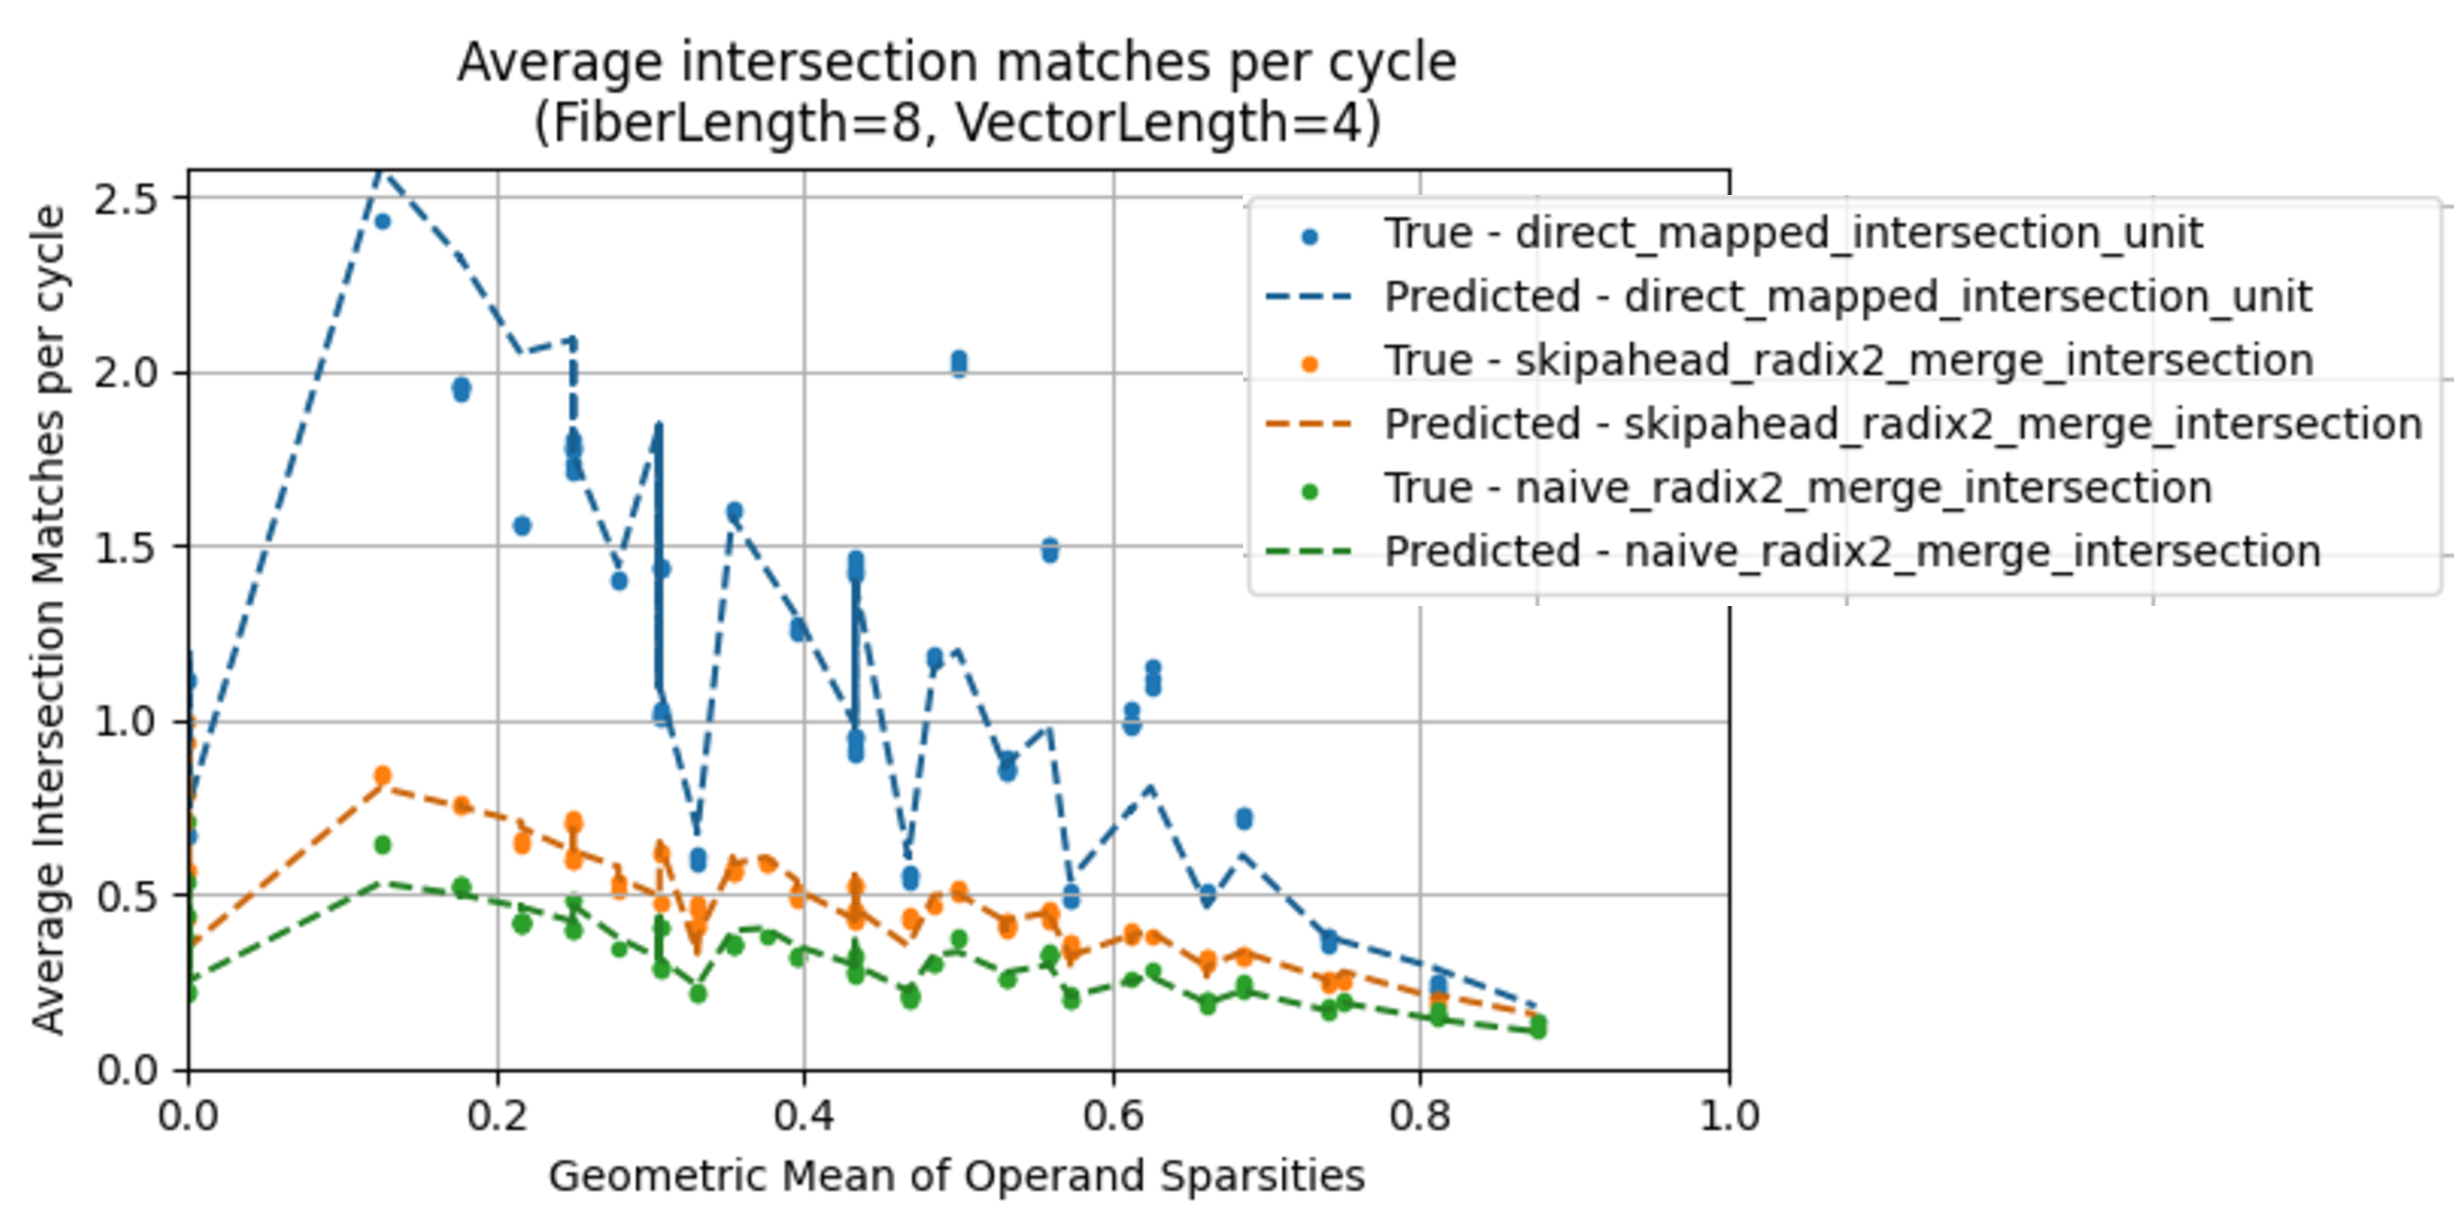
\includegraphics[width=0.95\textwidth]{figures/isect_model_fl8_vl4.pdf}
    \caption{Comparison of match throughput with respect to sparsity (geomean) for fiber size 8 and input vectorization 4. The predicted match throughput values from the analytical model developed for this work, are overlaid on simulated measurements from the intersection unit cycle accurate simulators. Additional analysis of this model is provided in Appendix~\ref{appendix:app_intersection_modeling}}
    \label{fig:isect_model_fl8_vl4}
\end{figure}

Note that the machine learning model relates the input workload - i.e. fiber sparsity, dense rank size - to the output workload - i.e. match throughput. Thus this machine learning model is the transfer relations for the bidirectional intersection SAF microarchitecture primitive. By passing this machine learning model through a computer algebra system, it was possible to obtain a symbolic representation of the transfer relation. This symbolic representation was integrated into the model definition.
%\chapter{SAF microarchitecture design space}

This section summarizes key design choices which form the SAF microarchitecture design space.

\section{SAF attributes}
%
% Figure: SAF attributes impact uarch cost
%
\begin{figure*}[ht]
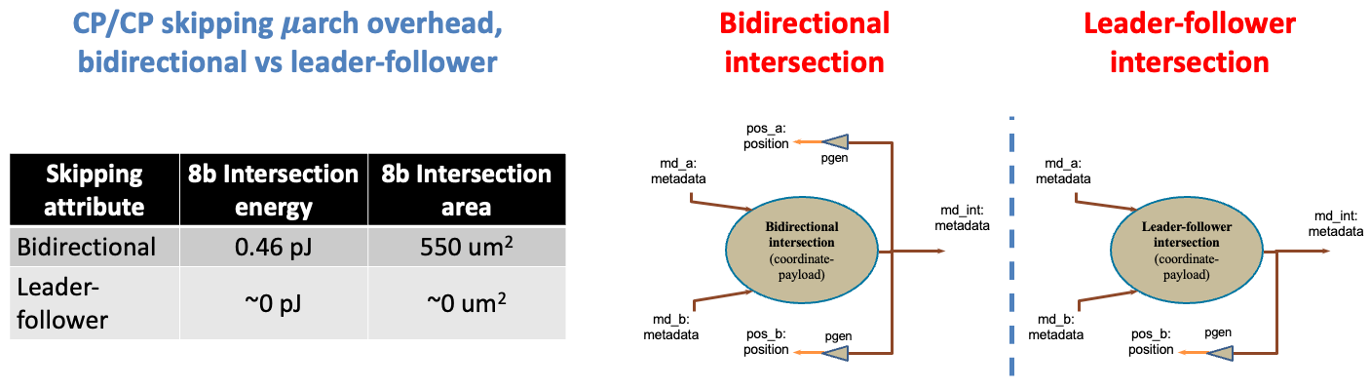
\includegraphics[width=\textwidth]{figures/saf_attributes_impact_uarch_cost.PNG}
\caption{Zero-skipping microarchitecture cost-comparison between an architecture with a bidirectional skipping SAF (left) and an architecture with a leader-follower skipping SAF (right.) Both architectures also employ a coordinate-payload format SAF.}
\label{fig:saf_attributes_impact_uarch_cost}
\centering
\end{figure*}
%
% Content: SAF attributes impact SAF microarchitecture cost
%
The attributes of a SAF impact the energy, area and latency of its SAF microarchitecture by implicitly constraining aspects of the design-space.
%
\subsection{SAF microarchitecture topology and primitive cost} 

Figure \ref{fig:saf_attributes_impact_uarch_cost} shows that a skipping SAF with the leader-follower attribute can have an implementation based on simple control logic that conditions MACs and follower reads on whether there is a nonzero leader operand. The energy and area overhead to implement this SAF is low. However designers may choose bidirectional skipping SAF instead in order to skip 100\% of ineffectual operations; this results in more expensive skipping microarchitecture with comparison logic to detect either or both zero operands, incurring a significant energy and area overhead. Generally, simple changes in the SAF optimization strategy may (or may not) have dramatic impact on microarchitecture complexity and thus on energy, area and latency.
%
\subsection{SAF primitive design}
%
\todo{Don't use terminology (i.e. primitive) which is not yet introduced.}
%
\section{Load-handling requirements}
%
\section{Optimizations}

\subsection{Algorithm}

\subsection{Pipelining}
%
\section{Cross-architecture impacts}


\chapter{SAF microarchitecture primitive taxonomy}
\label{chapter:primitive_taxo_model}

This section introduces a taxonomy of SAF microarchitecture primitives. Each taxonomic primitive expresses a basic operation that is key to implementing sparse tensor arithmetic, staying as close as possible to the \textit{Efficient Processing}\cite{szebook} taxonomy. 

The taxonomic system in this work is modeled off of C++ generics: 

\begin{itemize}
    \item This work defines a number of \textbf{taxonomic category templates} (or just \textit{categories}), which are analogous to \textit{C++ templates}. A taxonomic category in this work is parameterized by a set of \textbf{attributes}, which are analogous to \textit{template parameters} in C++ templates.
    \item A taxonomic category in this work is \textit{customized} by specifying attribute values, just as a \textit{C++ template customization} is the result of invoking a C++ template and specifying all of the template parameters. In this work, all possible legal combinations of attribute values for a given taxonomic category are referred to as the \textit{supported customizations} or just \textit{customizations} for that category.
    \item Within a given taxonomic category, there is \textbf{complete flexibility to adjust the primitive's RTL blocks, scale parameters, and constitutive relations for each customization}.
    \item To \textit{instantiate} a taxonomic primitive, is to realize a specific occurrence of the customized primitive within some design. \textit{Instantiation} in this work is analogous to \textit{instantiating} an object by calling the constructor for a particular template customization of a C++ class. In this work, instantiation is not possible unless all primitive attributes have been specified, i.e. a single customization has been unambiguously specified.
\end{itemize}

Conceptually, the taxonomic category describes a format-agnostic and broadly context-agnostic SAF microarchitecture primitive, while the category's customizations reflect that the primitive implementation is interdependent on format and characteristics of the surrounding design. This accomplishes the goal of keeping the taxonomy as format- and generally context-agnostic as possible (as discussed in Chapter~\ref{chapter:conceptual_framework} and also in \textit{Efficient Processing}\cite{szebook}); at the same time, the customizations make it easy to consider a primitive's more detailed implementation when it is necessary or helpful.

In addition to its taxonomic attributes, each SAF microarchitecture primitive is associated with:

\begin{itemize}
    \item \textbf{An interface}, comprising input and output ports. Each port has one of three \textit{Efficient Processing} interface types: \textit{metadata format}, \textit{position}, or \textit{flag}.
    \item \textbf{An analytical energy/area/timing model}, which is parameterized by the primitive's attributes.
\end{itemize}

By pairing each taxonomic primitive with an analytical model, we accomplish the goal described in Chapter~\ref{chapter:conceptual_framework} of evaluating and comparing designs.

In order to stay as close to the \textit{Efficient Processing} taxonomy as possible, it is desirable that the primitive's input and output ports can be understood as transmitting/receiving metadata, position or flag values. The ideal SAF microarchitecture primitive is domain-specific to tensor acceleration. Thus, SAF microarchitecture primitives are \textit{not} synonymous with RTL blocks from Chapter~\ref{chapter:rtl}, because RTL blocks are not \textit{necessarily} domain-specific in the way that SAF microarchitecture primitives are. A SAF microarchitecture primitive is constructed from zero or more RTL blocks.

In this work, the following rules are followed when deciding which SAF microarchitecture primitive characteristics should be captured as taxonomic attributes, versus which characteristics should be captured as scale parameters:

\begin{itemize}
    \item \textbf{Does the characteristic in question distinguish paradigmatically different approaches to implementing the primitive functionality?} Example: tree vs ripple implementation is a good candidate for a taxonomic attribute. Counter-example: most low-level pipelining decisions, unless they impact scaling behavior, should be scaling parameters in the primitive model, if they are even represented at all.
    \item \textbf{Does the characteristic in question impact the \textit{shape of the component's scaling trend}?} Example: pipelining a multi-step operation over multiple pipeline stages, versus combinationally unrolling multiple iterations of the operation within a single pipeline stage; this distinction is a good candidate for a taxonomic attribute since it strongly impacts the scaling behavior of propagation delay, and by extension the feasibility of the design. Counter-example: the particular choice of metadata word bitwidth does not change the \textit{shape} of the primitive's scaling behavior, however it \textit{does} select a particular point on the scaling curve, and so is an excellent candidate for a scaling parameter.
\end{itemize}

The following sections will introduce the SAF microarchitecture primitive categories developed for this work. 

For brevity, the analytical model definitions will not be provided for the primitives in this section. However, the transfer relation model for coordinate-payload intersection, developed in Section~\ref{sec:c_c_isect_modeling}, is an example of how to go about building analytical models of SAF microarchitecture primitives.

\section{Metadata parser taxonomic category template}

\begin{figure}[H]
    \centering
    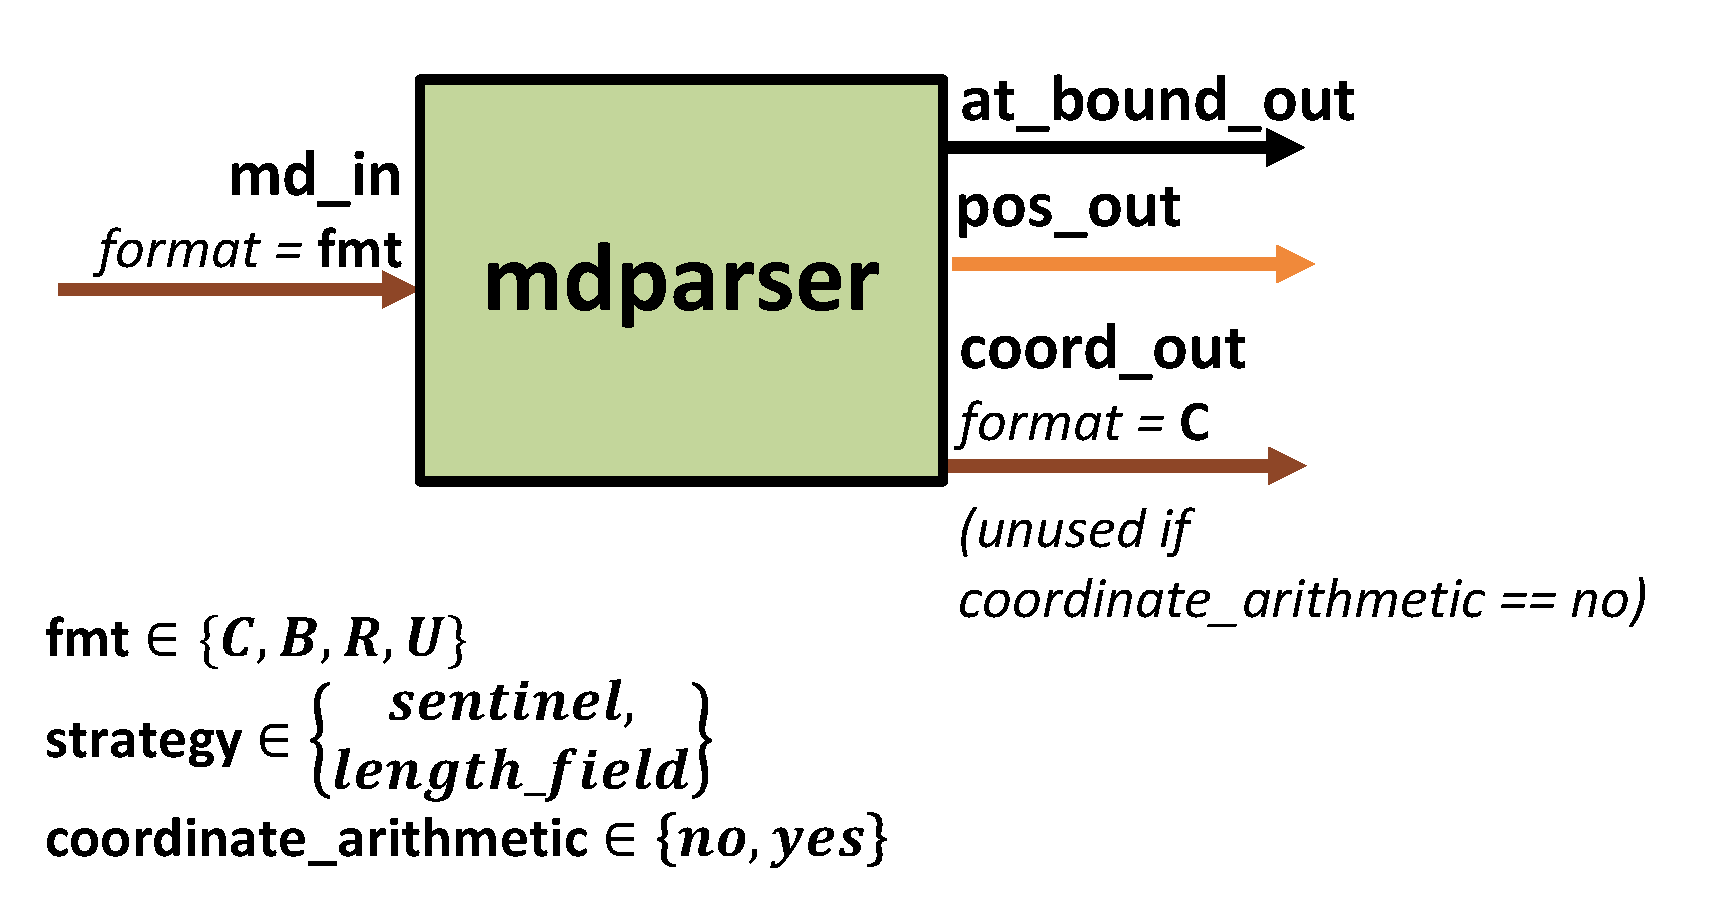
\includegraphics[width=0.95\textwidth]{figures/mdparser.pdf}
    \caption{Metadata parser primitive component template.}
    \label{fig:mdparser}
\end{figure}

The metadata parser SAF microarchitecture primitive (mdparser) follows the functionality described in Section~\ref{chapter:conceptual_framework}, parsing sparse format metadata and outputting (1) positional offsets for looking up payloads (\textit{pos\_out}) and (2) reset signals at the end of fiber traversal (\textit{at\_bound\_out}.) Additionally, for implicit coordinate formats, the metadata parser can \textit{optionally} compute explicit coordinates to support coordinate coordinate computation.

The metadata parser primitive attributes are

\begin{itemize}
    \item \textbf{format -} The sparse representation format supported by the metadata parser.
    \item \textbf{strategy -} The strategy employed by the metadata parser for detecting the end of traversal.
    \begin{itemize}
        \item \textbf{sentinel -} a sentinel symbol is detected at the end of the fiber (depending on the format, the symbol may appear at the end of the metadata, or at the end of the fiber payload array.)
        \item \textbf{length\_field -} the fiber metadata includes a value which is the length of the fiber (depending on the format, this may be the length of the metadata array, or the length of the payload array.)
    \end{itemize}
    \item \textbf{coordinate\_arithmetic -} \textit{yes} if the metadata parser must compute explicit coordinates, \textit{no} otherwise.
\end{itemize}

The supported metadata parser specializations are shown in Table~\ref{tab:MetadataParser_specializations}.

\begin{table}[H]
\centering
\begin{tabular}{lll}
\toprule
 format   & strategy       & coordinate\_arithmetic   \\
\midrule
 U        & sentinel & no\_arithmetic                \\
 U        & sentinel & yes\_arithmetic                 \\
 U        & length\_field & no\_arithmetic              \\
 U        & length\_field & yes\_arithmetic             \\
 C        & sentinel & no\_arithmetic                \\
 C        & sentinel & yes\_arithmetic                 \\
 C        & length\_field & no\_arithmetic              \\
 C        & length\_field & yes\_arithmetic             \\
 B        & sentinel & no\_arithmetic                  \\
 B        & sentinel & yes\_arithmetic                 \\
 B        & length\_field & no\_arithmetic              \\
 B        & length\_field & yes\_arithmetic             \\
\bottomrule
\end{tabular}
\caption{Specializations of metadata parsers.}
\label{tab:MetadataParser_specializations}
\end{table}

\section{Coupled position generators}

Recall from Section~\ref{chapter:conceptual_framework} that \textit{coupled} position generators output position offsets in payload memory, conditional on metadata values provided as input. Thus coupled position generators are classified as SAF microarchitecture.

\subsection{Single position generator taxonomic category template}

\begin{figure}[H]
    \centering
    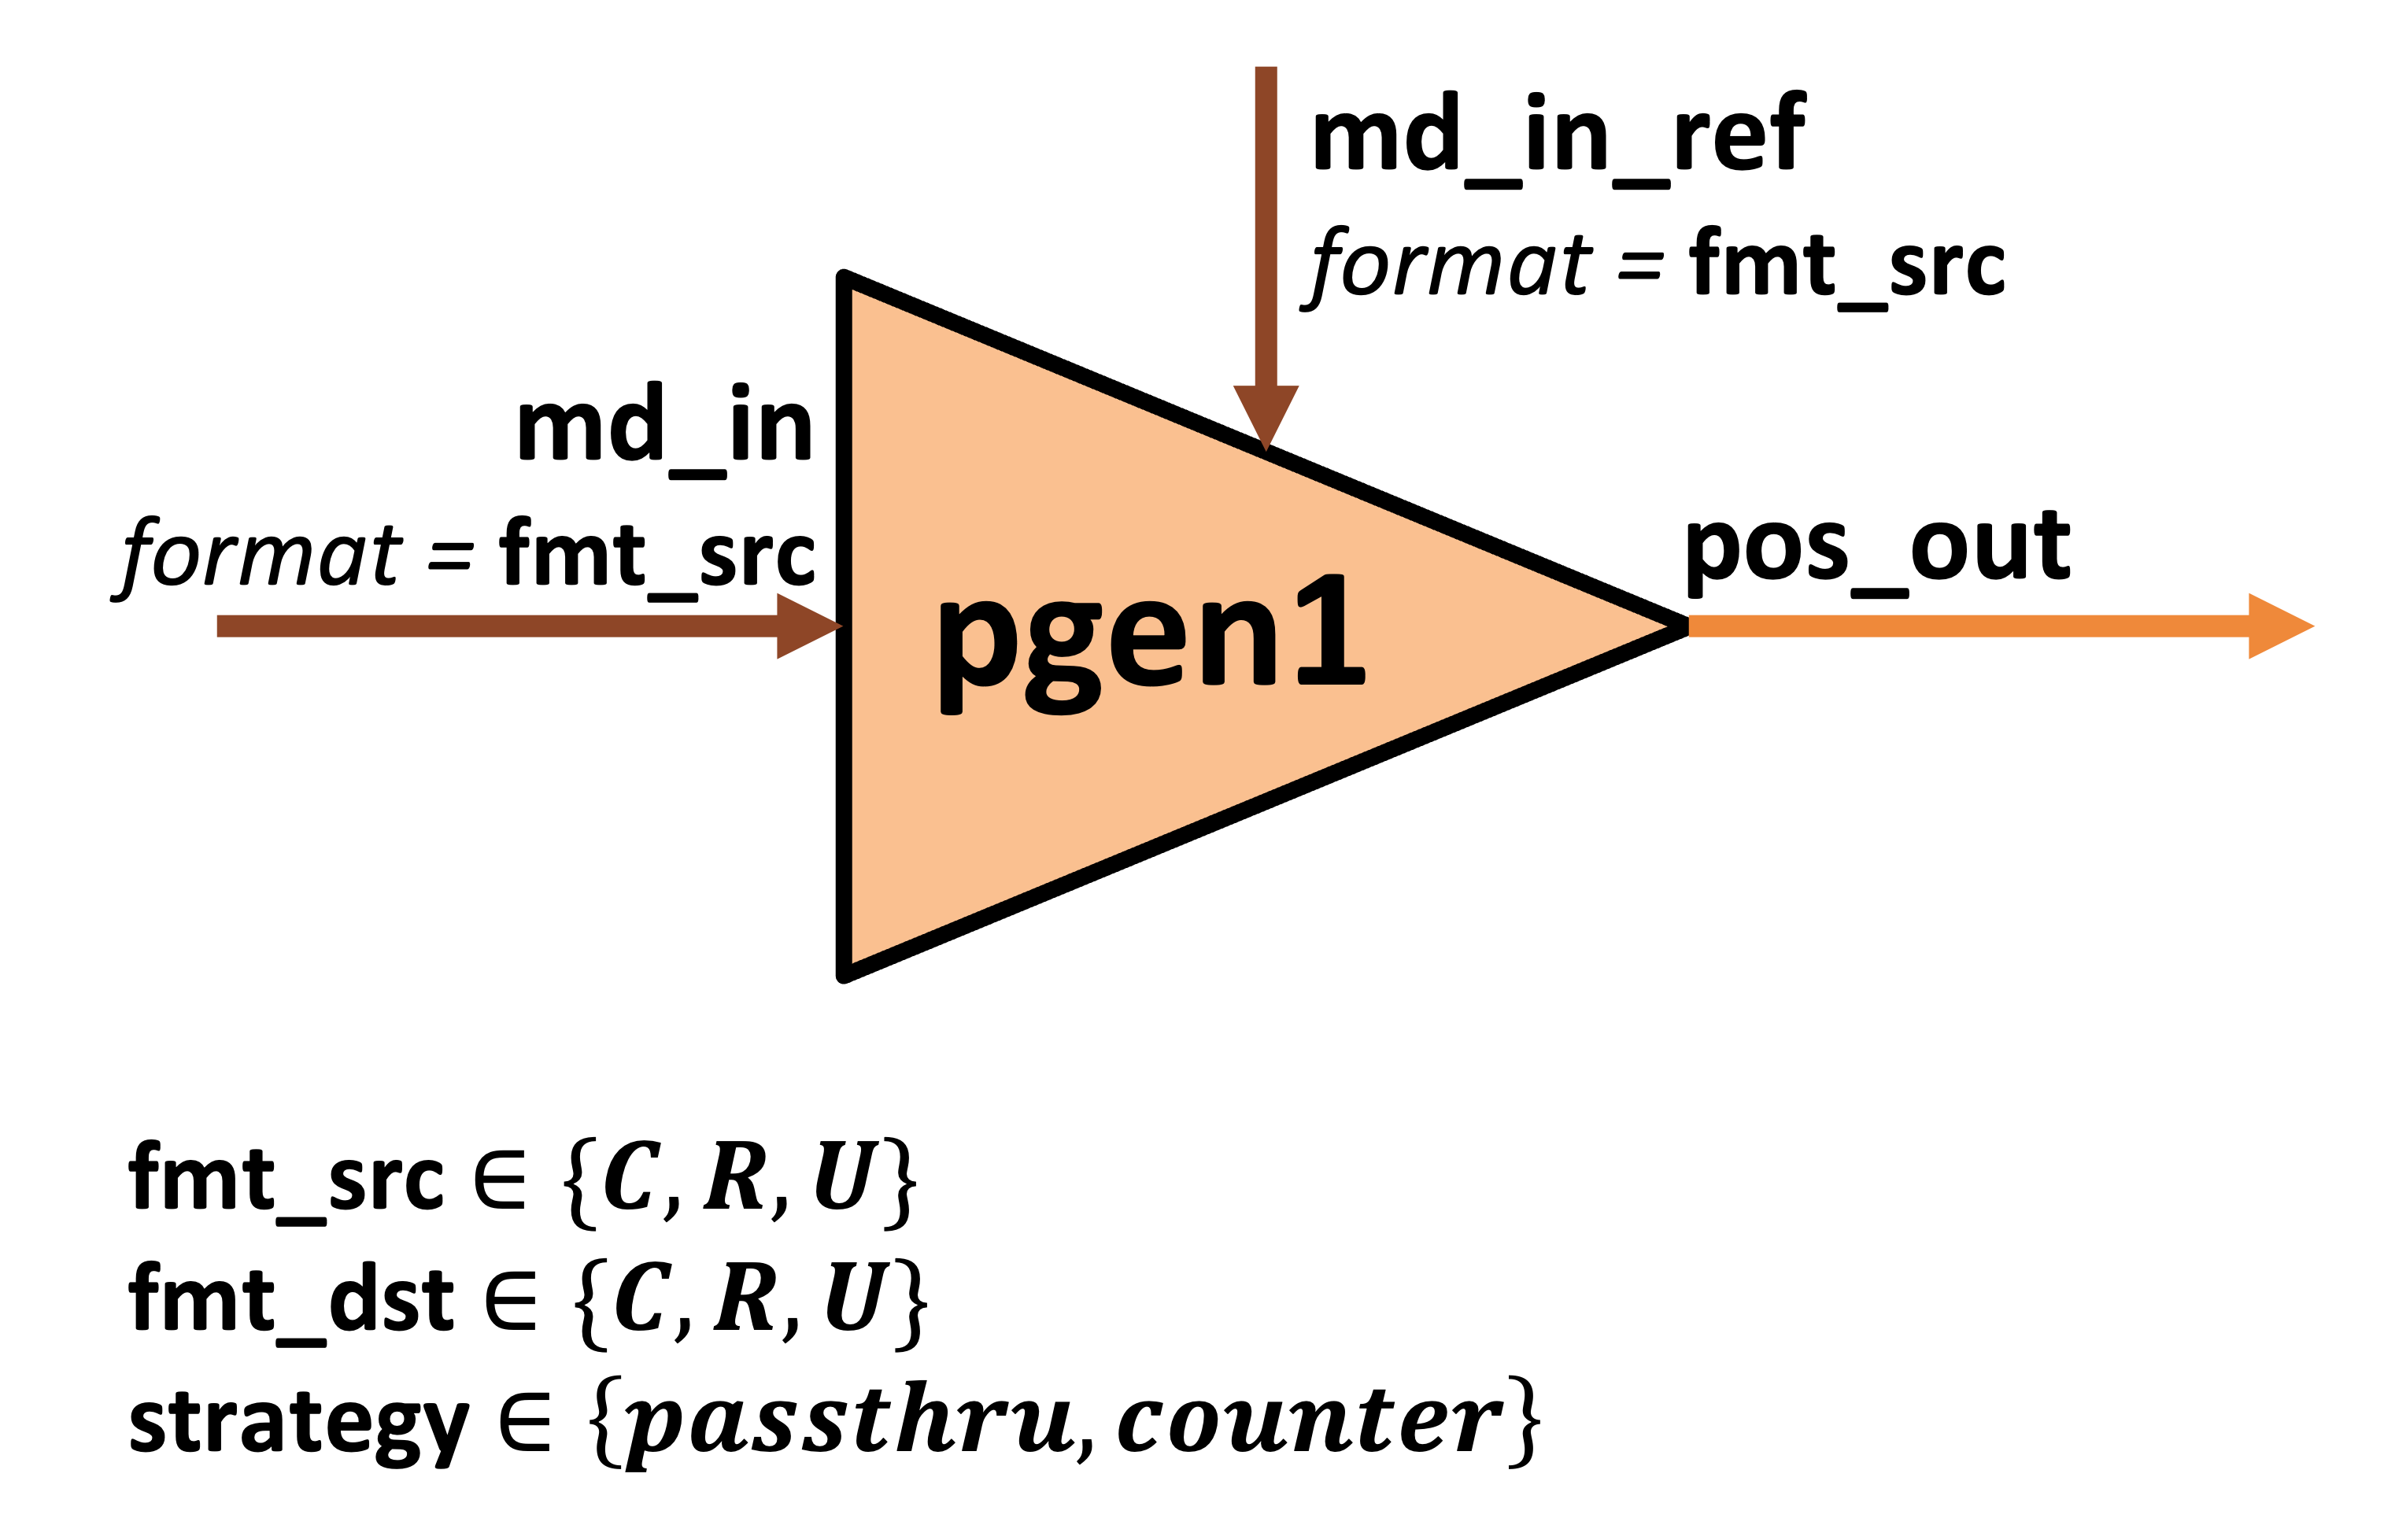
\includegraphics[width=0.95\textwidth]{figures/pgen1.png}
    \caption{Single position generator primitive component template.}
    \label{fig:pgen1}
\end{figure}

The Single position generator (pgen1, Figure~\ref{fig:pgen1}) converts a single metadata input stream into a single position offset output stream. It is used, for example, in coordinate-payload bidirectional skipping microarchitectures, as described in Section~\ref{chapter:conceptual_framework}.

Depending on the particular customization (i.e. the \textit{counter}-based strategy), the pgen1 may exploit the reference input (\textit{md\_in\_ref}), computing positional offsets based on comparing the primary metadata input to the reference input.

However, the \textit{passthrough} strategy is simply a wire directly from the primary metadata input to the position output, so the reference input is not utilized for this strategy.

Which strategies are valid, is dependent on (1) the format of the input metadata and (2) the format of the fiber which the position offsets will index into. The pgen1 has the following attributes:

\begin{itemize}
    \item \textbf{format\_src -} The format of the ``source'' fiber which originates the metadata input.
    \item \textbf{format\_dst -} The format of the ``destination'' fiber, which the positional offsets generated at the output will index into.
    \item \textbf{strategy -} The approach to implementing position offset generation. Strongly influences whether and how the reference input is utilized.
    \begin{itemize}
        \item \textbf{passthrough -} Wire directly from primary metadata input to position output; reference input is not utilized.
        \item \textbf{counter -} Each metadata value arriving at the reference input increments a counter (the amount of increment is equal to the input vectorization of the pgen1 unit, which is a lower-level scale parameter.) When a metadata value arrives at the primary input, the pgen1 outputs the counter value. This represents the scenario in which the primary input is connected to an coordinate-payload intersection unit's output, and the reference input is connected to one of the skipping microarchitecture's input metadata streams; the output position offsets represent the index of the matching metadata values, within the particular input metadata stream.
    \end{itemize}
\end{itemize}

Single position generator specializations are shown in Table~\ref{tab:SinglePositionGenerator_specializations}.

\begin{table}[H]
\centering
\begin{tabular}{lll}
\toprule
 format\_src   & format\_dst   & strategy    \\
\midrule
 C            & U            & passthrough \\
 C            & C            & counter     \\
\bottomrule
\end{tabular}
\caption{Specializations of Single position-generator}
\label{tab:SinglePositionGenerator_specializations}
\end{table}

\subsection{Dual position generator taxonomic category template}

\begin{figure}[H]
    \centering
    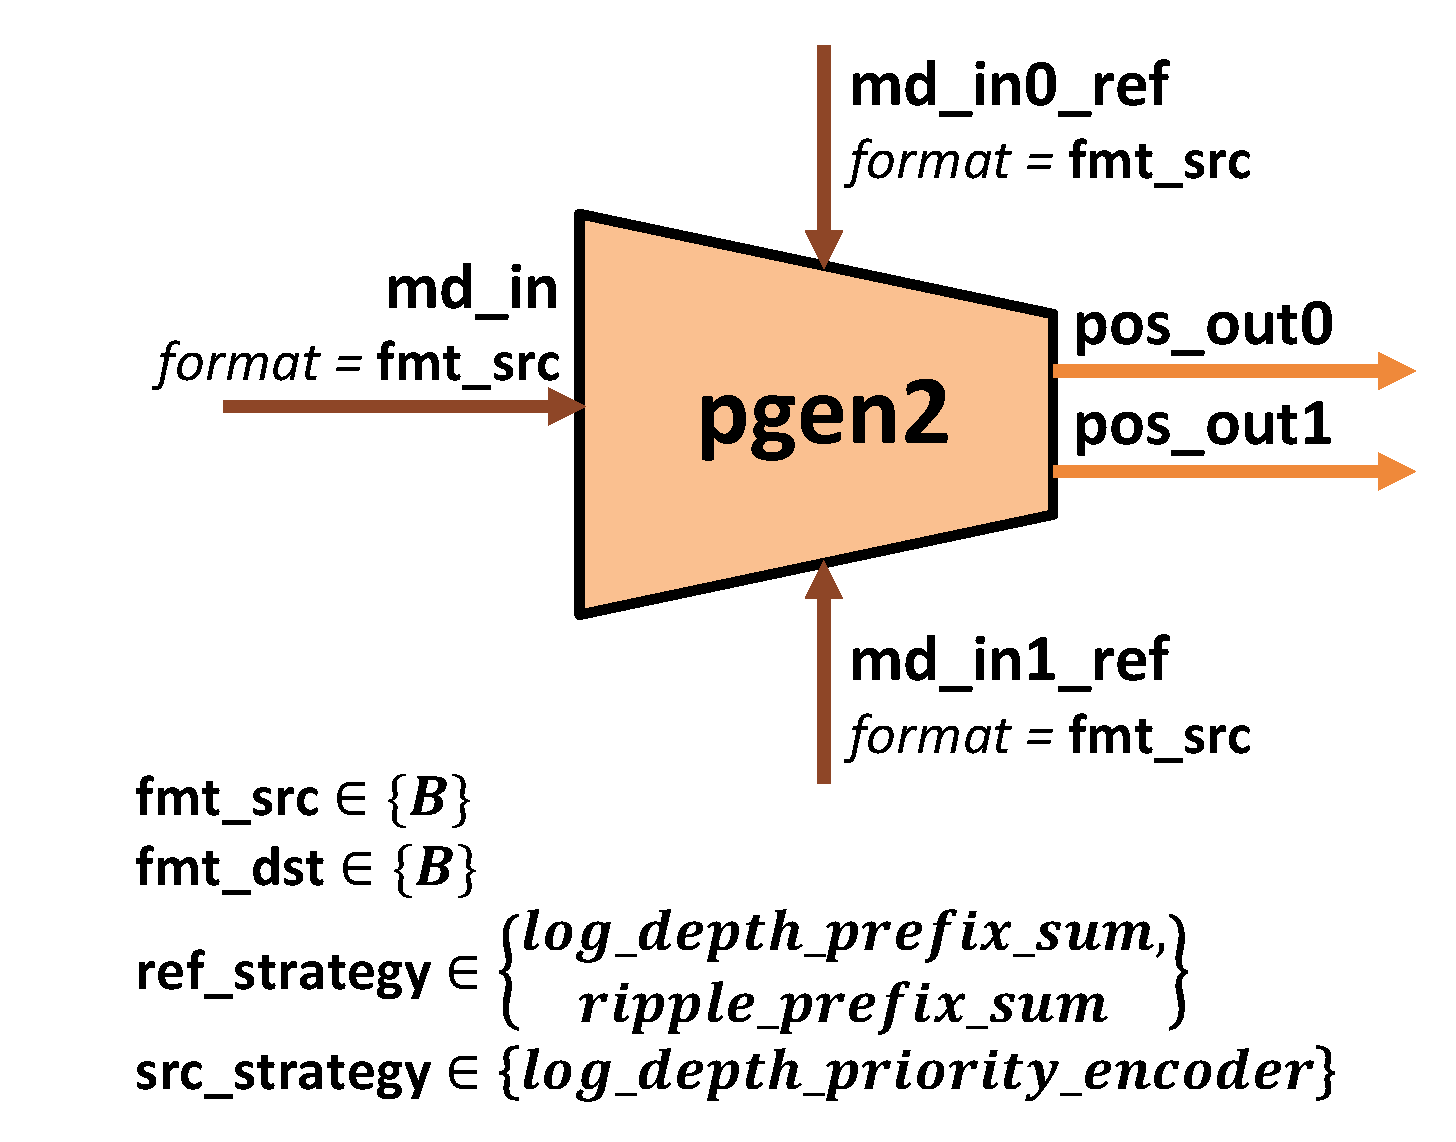
\includegraphics[width=0.95\textwidth]{figures/pgen2.pdf}
    \caption{Dual position generator primitive component template.}
    \label{fig:pgen2}
\end{figure}

The Dual position generator (pgen2, Figure~\ref{fig:pgen2}) converts a single metadata input stream into a two position offset output streams. pgen2 is utilized, for example, in bitmask intersection units, as described in Section~\ref{chapter:conceptual_framework}.

Like pgen1, pgen2 has a single metadata input; unlike pgen1, pgen2 has two reference inputs and two positional offset outputs. 

pgen2 compares the primary metadata input, to both of the reference inputs; the comparison to the first reference input yields the first position offset output stream, and the comparison to the second reference input yields the second position offset output stream.

pgen2 assumes that all metadata inputs are sourced from fibers of the same representation format, and that both positional outputs are indexing into fibers with the same representation format.

The pgen2 has the following attributes -

\begin{itemize}
    \item \textbf{format\_src -} The format of the ``source'' fibers which originate the metadata inputs.
    \item \textbf{format\_dst -} The format of the ``destination'' fibers, which the positional offsets generated at the output will index into.
    \item \textbf{reference\_strategy -} The strategy for processing the reference metadata inputs. When format\_src is Bitmask (B), then reference\_strategy reflects the choice of RTL block used for computing prefix-sum of the reference metadata input streams. The options are:
    \begin{itemize}
        \item \textbf{ripple\_prefix\_sum }
        \item \textbf{kogge\_stone\_prefix\_sum}
    \end{itemize}
    These options refer to prefix-sum RTL blocks in Section~\ref{chapter:rtl}.
    \item \textbf{source\_strategy -} The strategy for processing the primary metadata input. If format\_src is Bitmask (B), then source\_strategy reflects the choice of RTL block used for priority encoder. The options are
    \begin{itemize}
        \item \textbf{parallel\_dec2\_priority\_encoder }
        \item A ripple priority encoder option would be interesting to explore but was not investigated in this work.
    \end{itemize}
\end{itemize}

Dual position generator specializations are shown in Table~\ref{tab:DualPositionGenerator_specializations}.

\begin{table}[H]
\centering
\begin{tabular}{llll}
\toprule
 format\_src   & format\_dst   & reference\_strategy        & source\_strategy             \\
\midrule
 B            & B            & ripple\_prefix\_sum      & parallel\_dec2\_priority\_encoder \\
 B            & B            & kogge\_stone\_prefix\_sum & parallel\_dec2\_priority\_encoder \\
\bottomrule
\end{tabular}
\caption{Specializations of dual position generator}
\label{tab:DualPositionGenerator_specializations}
\end{table}

\section{Intersection units}

Intersection units intersect two fibers and output a stream of metadata representing matches. The meaning of the match stream reflects the type of join being performed.

\subsection{Leader-follower intersection unit taxonomic category template}

The \textit{md\_in\_leader} input is the sparse metadata associated with the leader operand; the \textit{md\_out} output produces a stream of metadata corresponding to matches; see Figure~\ref{fig:isectlf}.

Leader-follower intersections perform a left-outer join between two fibers; thus, the output match stream reflects \textit{all} of the leader metadata, but only that follower metadata which matches the leader.

\begin{figure}[H]
    \centering
    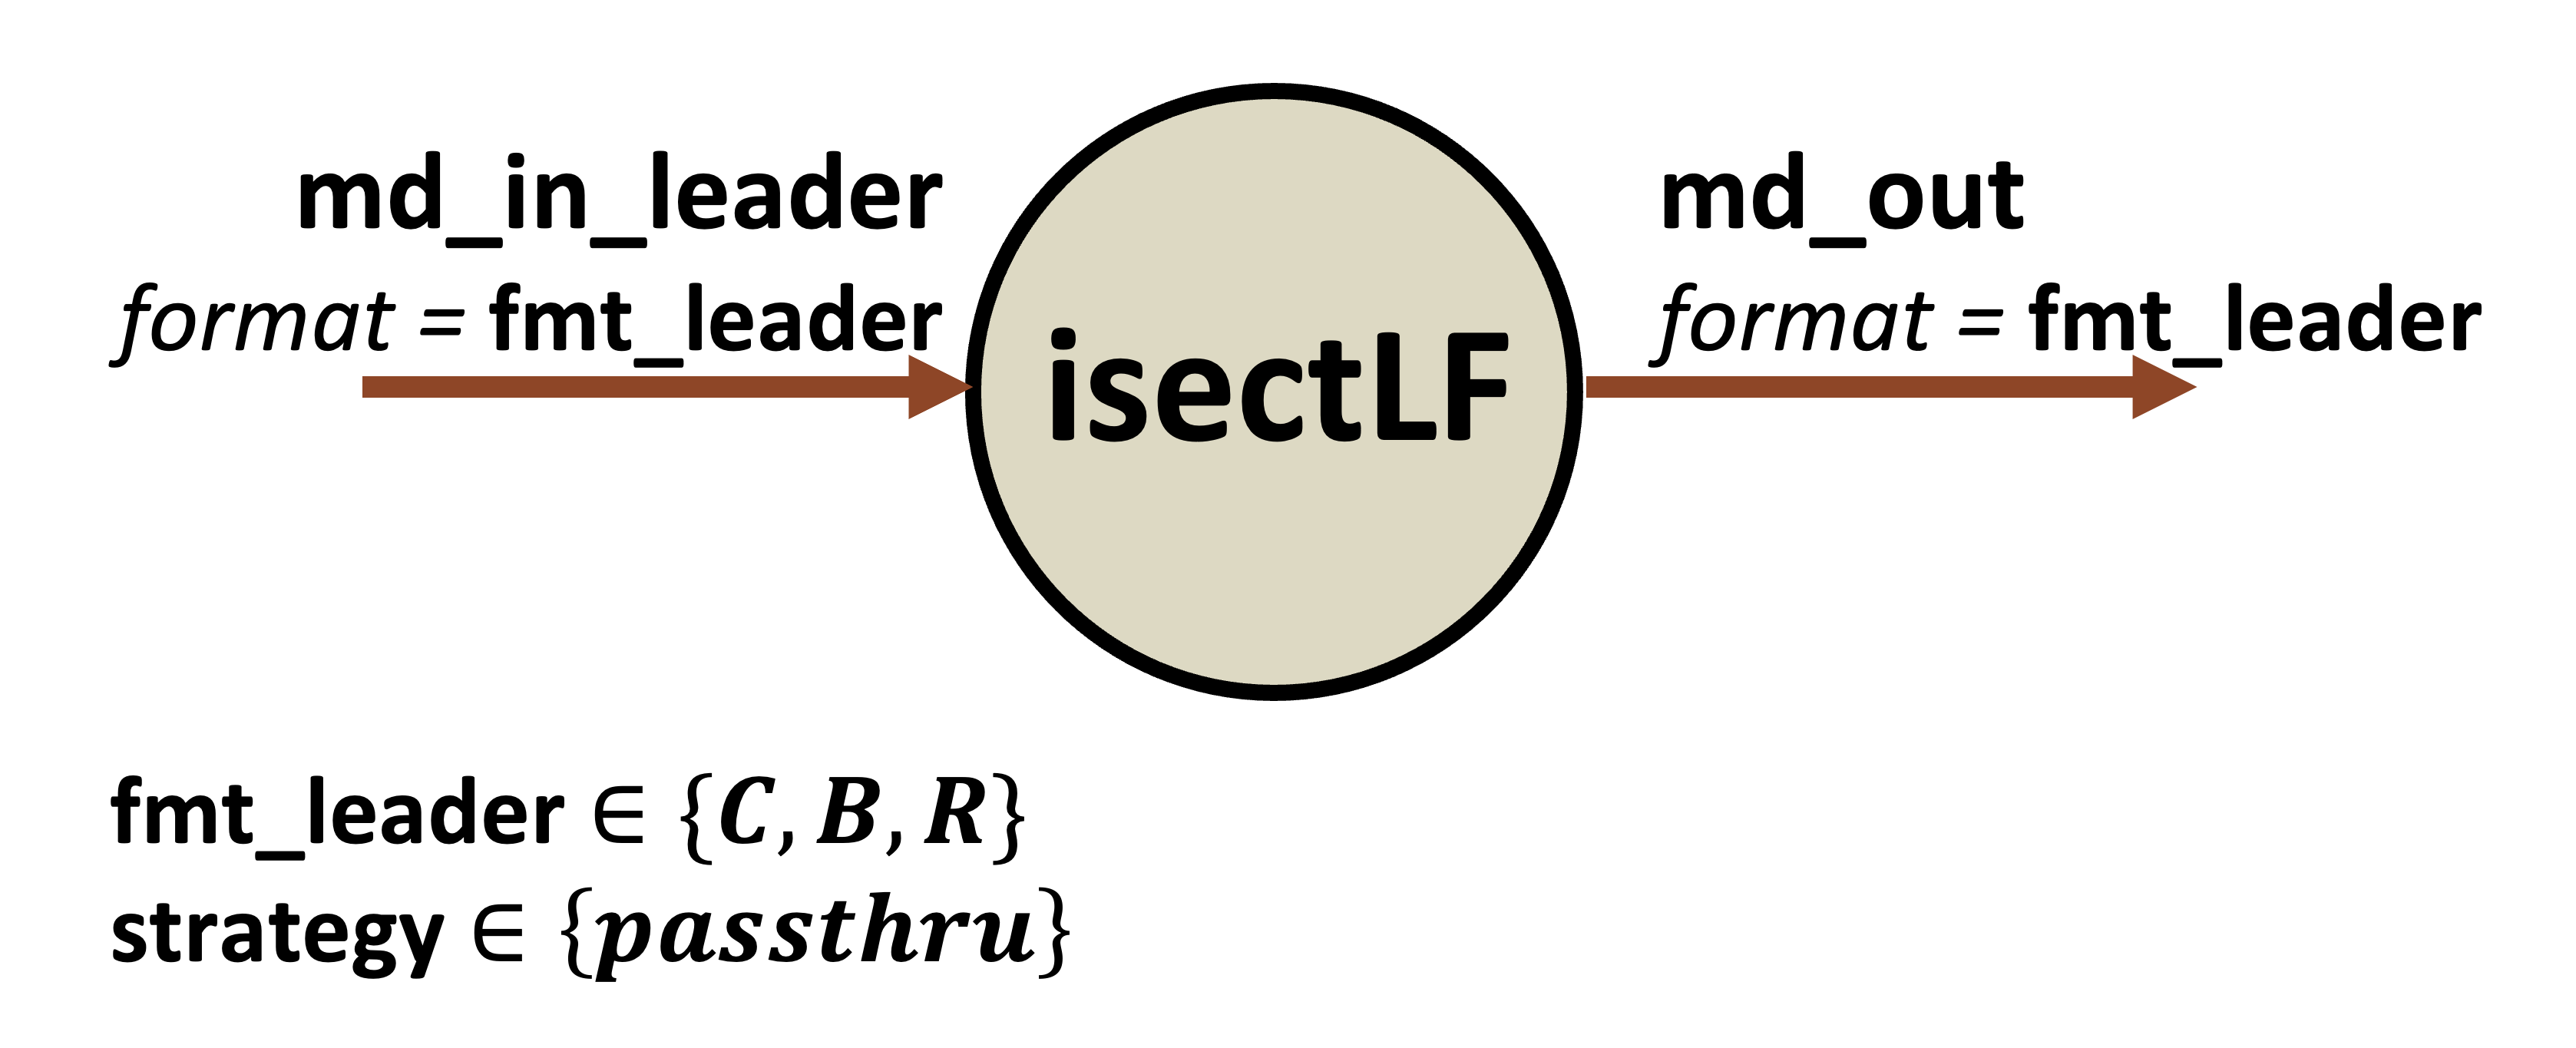
\includegraphics[width=0.95\textwidth]{figures/isectlf.png}
    \caption{Leader-follower intersection primitive component template.}
    \label{fig:isectlf}
\end{figure}

The leader-follower intersection SAF microarchitecture primitive attributes are:

\begin{itemize}
    \item \textbf{format\_leader -} The leader fiber sparse representation format.
    \item \textbf{strategy -} All leader-follower intersections implement a \textit{passthrough} strategy, i.e. a wire directly from input to output.
\end{itemize}

The supported customizations for leader-follower intersection are shown in Table~\ref{tab:IntersectionLeaderFollower_specializations}.

\begin{table}[H]
\centering
\begin{tabular}{ll}
\toprule
 format\_leader   & strategy    \\
\midrule
 C               & passthrough \\
 B               & passthrough \\
\bottomrule
\end{tabular}
\caption{Specializations of leader-follower intersection.}
\label{tab:IntersectionLeaderFollower_specializations}
\end{table}

\subsection{Bidirectional intersection unit taxonomic category template}

For bidirectional intersection unit, the \textit{md\_in0} and \textit{md\_in1} inputs receive sparse format metadata from the two fibers being intersected; the \textit{md\_out} output produces a stream of metadata corresponding to matches; see Figure~\ref{fig:isectbd}.

Bidirectional intersections perform an inner join between two fibers; thus, the output match stream reflects \textit{only} the metadata for coordinates which are common to both fibers.

\begin{figure}[H]
    \centering
    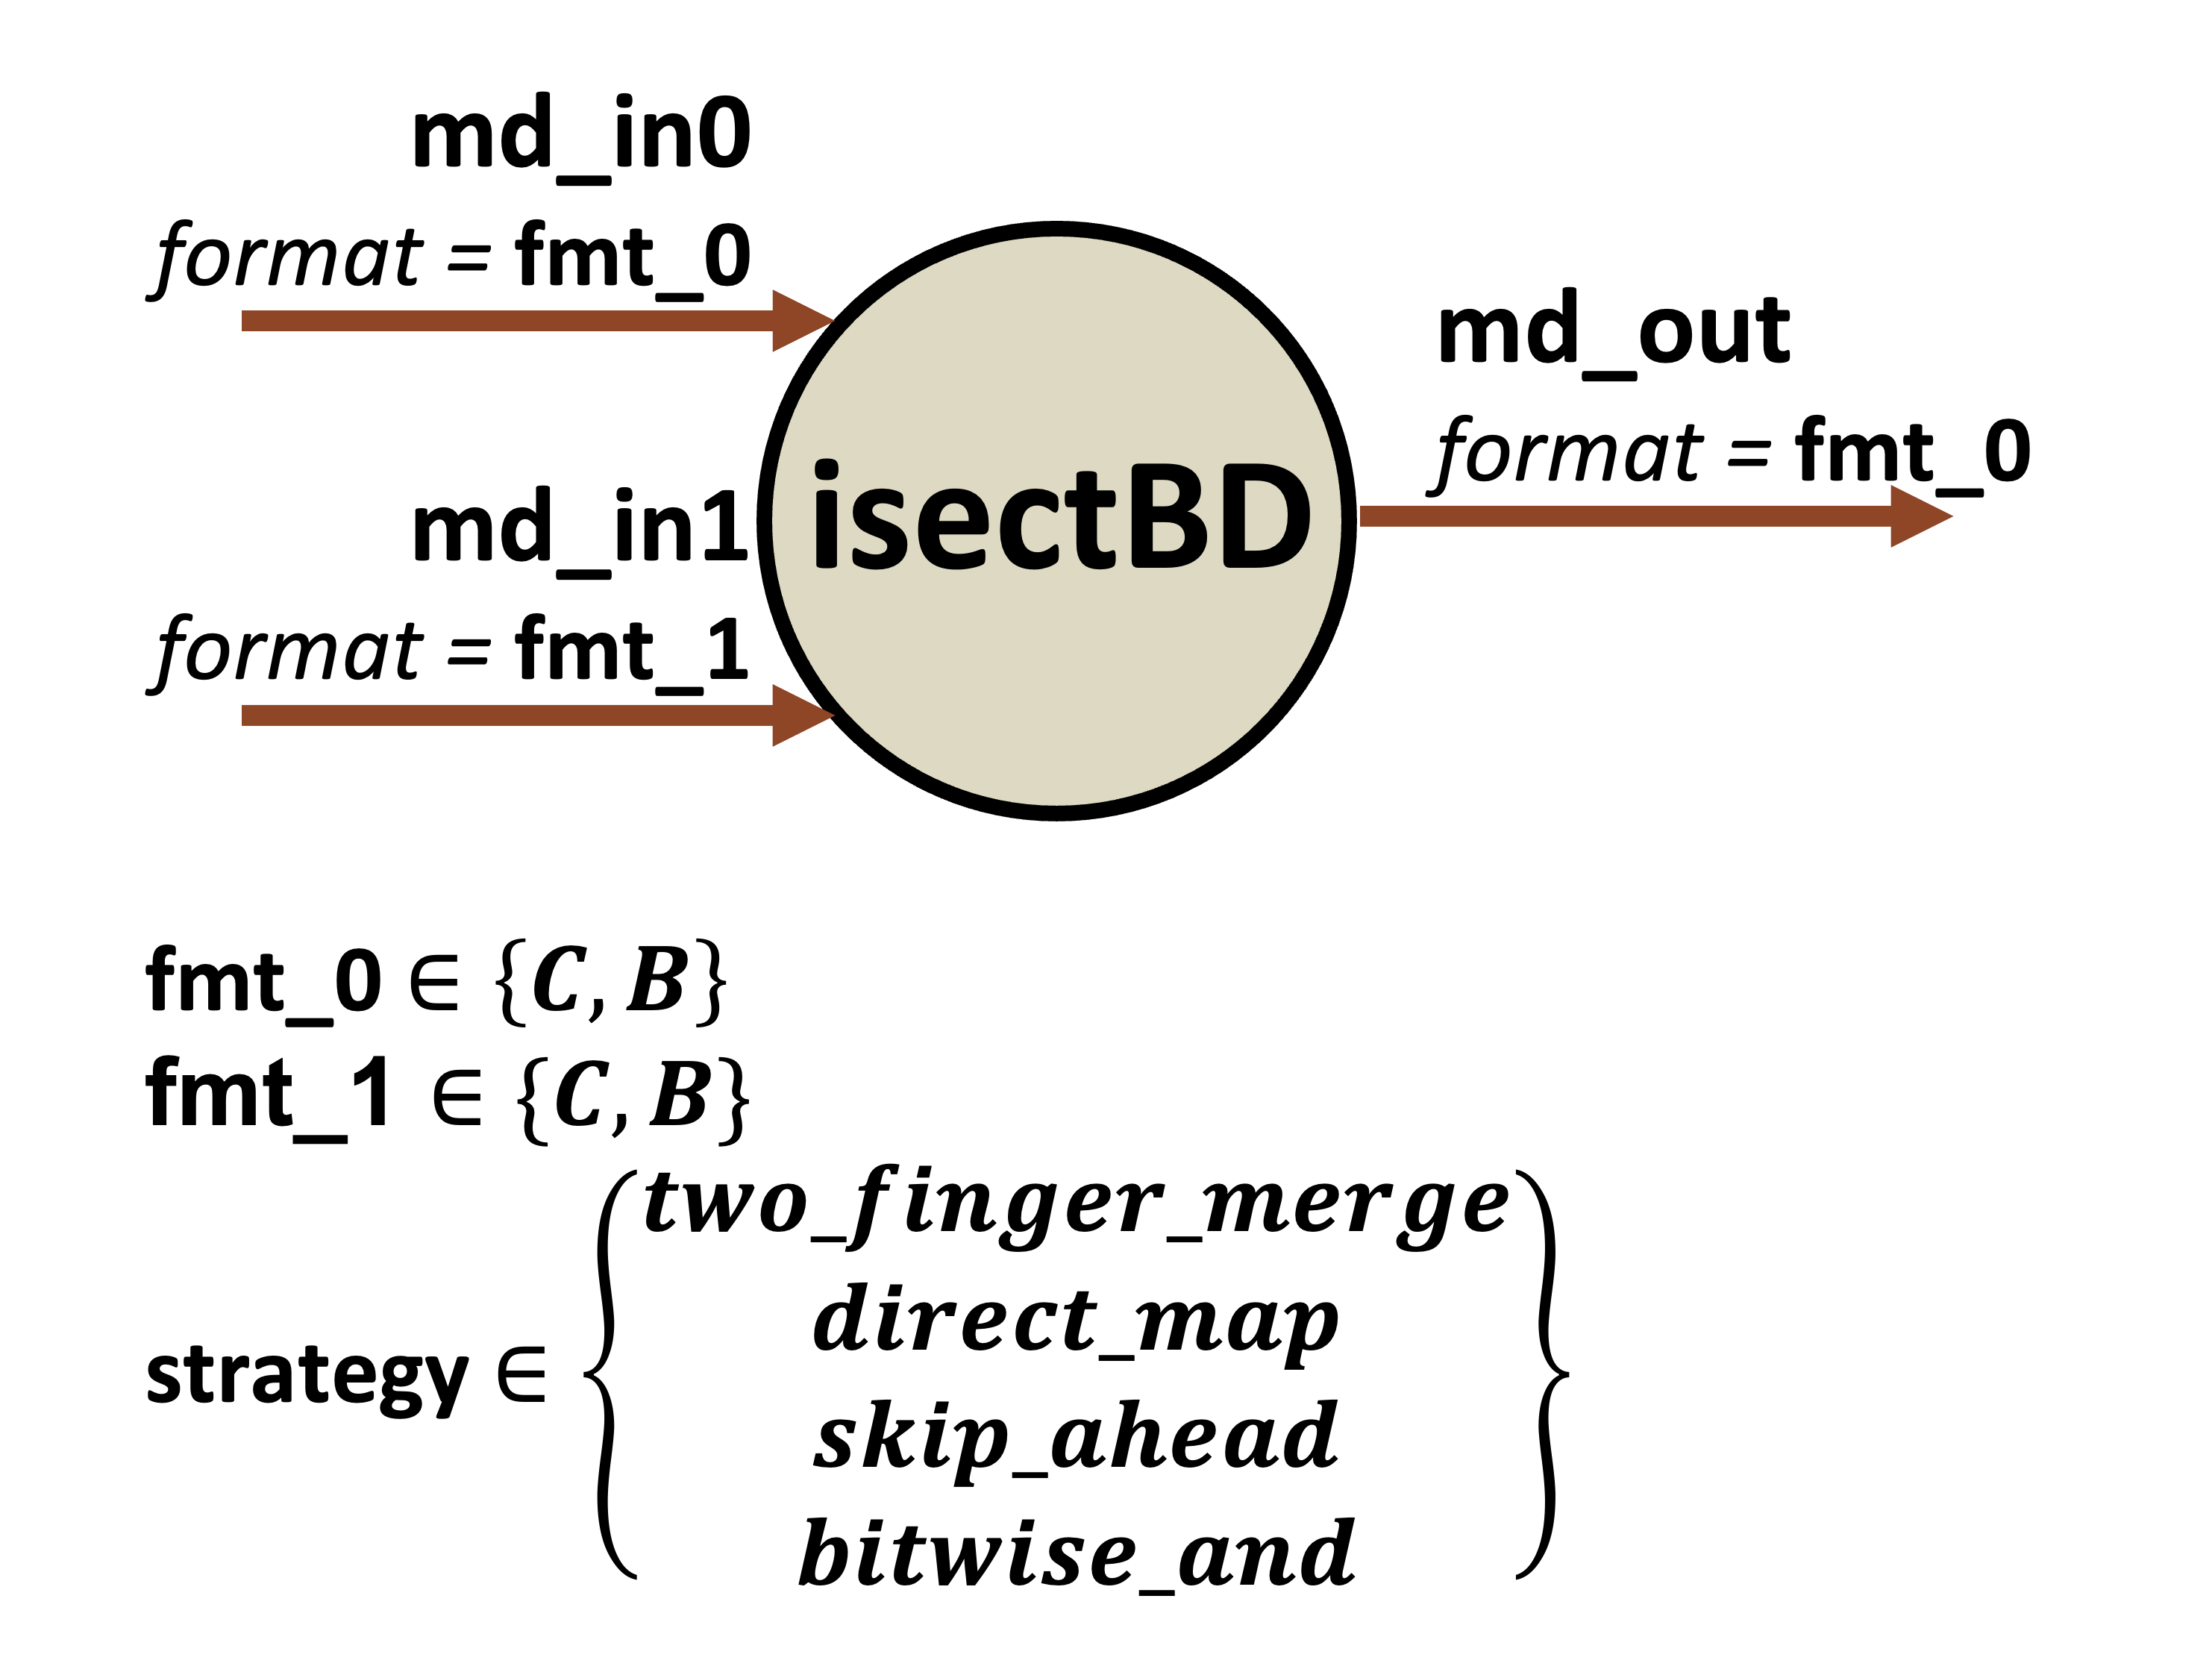
\includegraphics[width=0.95\textwidth]{figures/isectbd.png}
    \caption{Bidirectional intersection primitive component template.}
    \label{fig:isectbd}
\end{figure}

The attributes of a bidirectional intersection unit are

\begin{itemize}
    \item \textbf{format\_0}, \textbf{format\_1 -} The formats of the two input fibers being intersected.
    \item \textbf{strategy -} The approach to implementing bidirectional intersection. \textit{strategy} is effectively selecting an intersection unit RTL block from Section~\ref{chapter:rtl}.
    \begin{itemize}
        \item \textbf{two\_finger\_merge -} ExTensor-like\cite{extensor} naive two-finger coordinate-payload intersection unit.
        \item \textbf{skip\_ahead -} ExTensor-like\cite{extensor} optimized coordinate-payload intersection unit.
        \item \textbf{direct\_map -} The direct-mapped coordinate-payload intersection unit, developed for this work.
        \item \textbf{bitwise\_and -} A SparTen-like\cite{sparten} bitmask intersection unit.
    \end{itemize}
\end{itemize}

The supported specializations for bidirectional intersection unit are shown in Table~\ref{tab:IntersectionBidirectional_specializations}.

\begin{table}[H]
\centering
\begin{tabular}{lll}
\toprule
 format\_0   & format\_1   & strategy         \\
\midrule
 C          & C          & two\_finger\_merge \\
 C          & C          & skip\_ahead       \\
 C          & C          & direct\_map       \\
 B          & B          & bitwise\_and      \\
\bottomrule
\end{tabular}
\caption{Specializations of bidirectional intersection.}
\label{tab:IntersectionBidirectional_specializations}
\end{table}

\section{Fill optimizer taxonomic category template}

The function of Fill optimizers (Figure~\ref{fopt}) is discussed in Section~\ref{chapter:conceptual_framework}. The Fill optimizer's (fopt's) method for discarding payload fills - as well as the interface between the fopt and the payload stream - is highly implementation-dependent, thus the fopt template does not have a ``payload'' interface. The red dotted line from fopt to payload stream (Figure~\ref{fopt}) is a visual cue for which payload stream is being optimized, but in actuality \textit{pos\_in} is the only interface port defined for this primitive component template.

\begin{figure}[H]
    \centering
    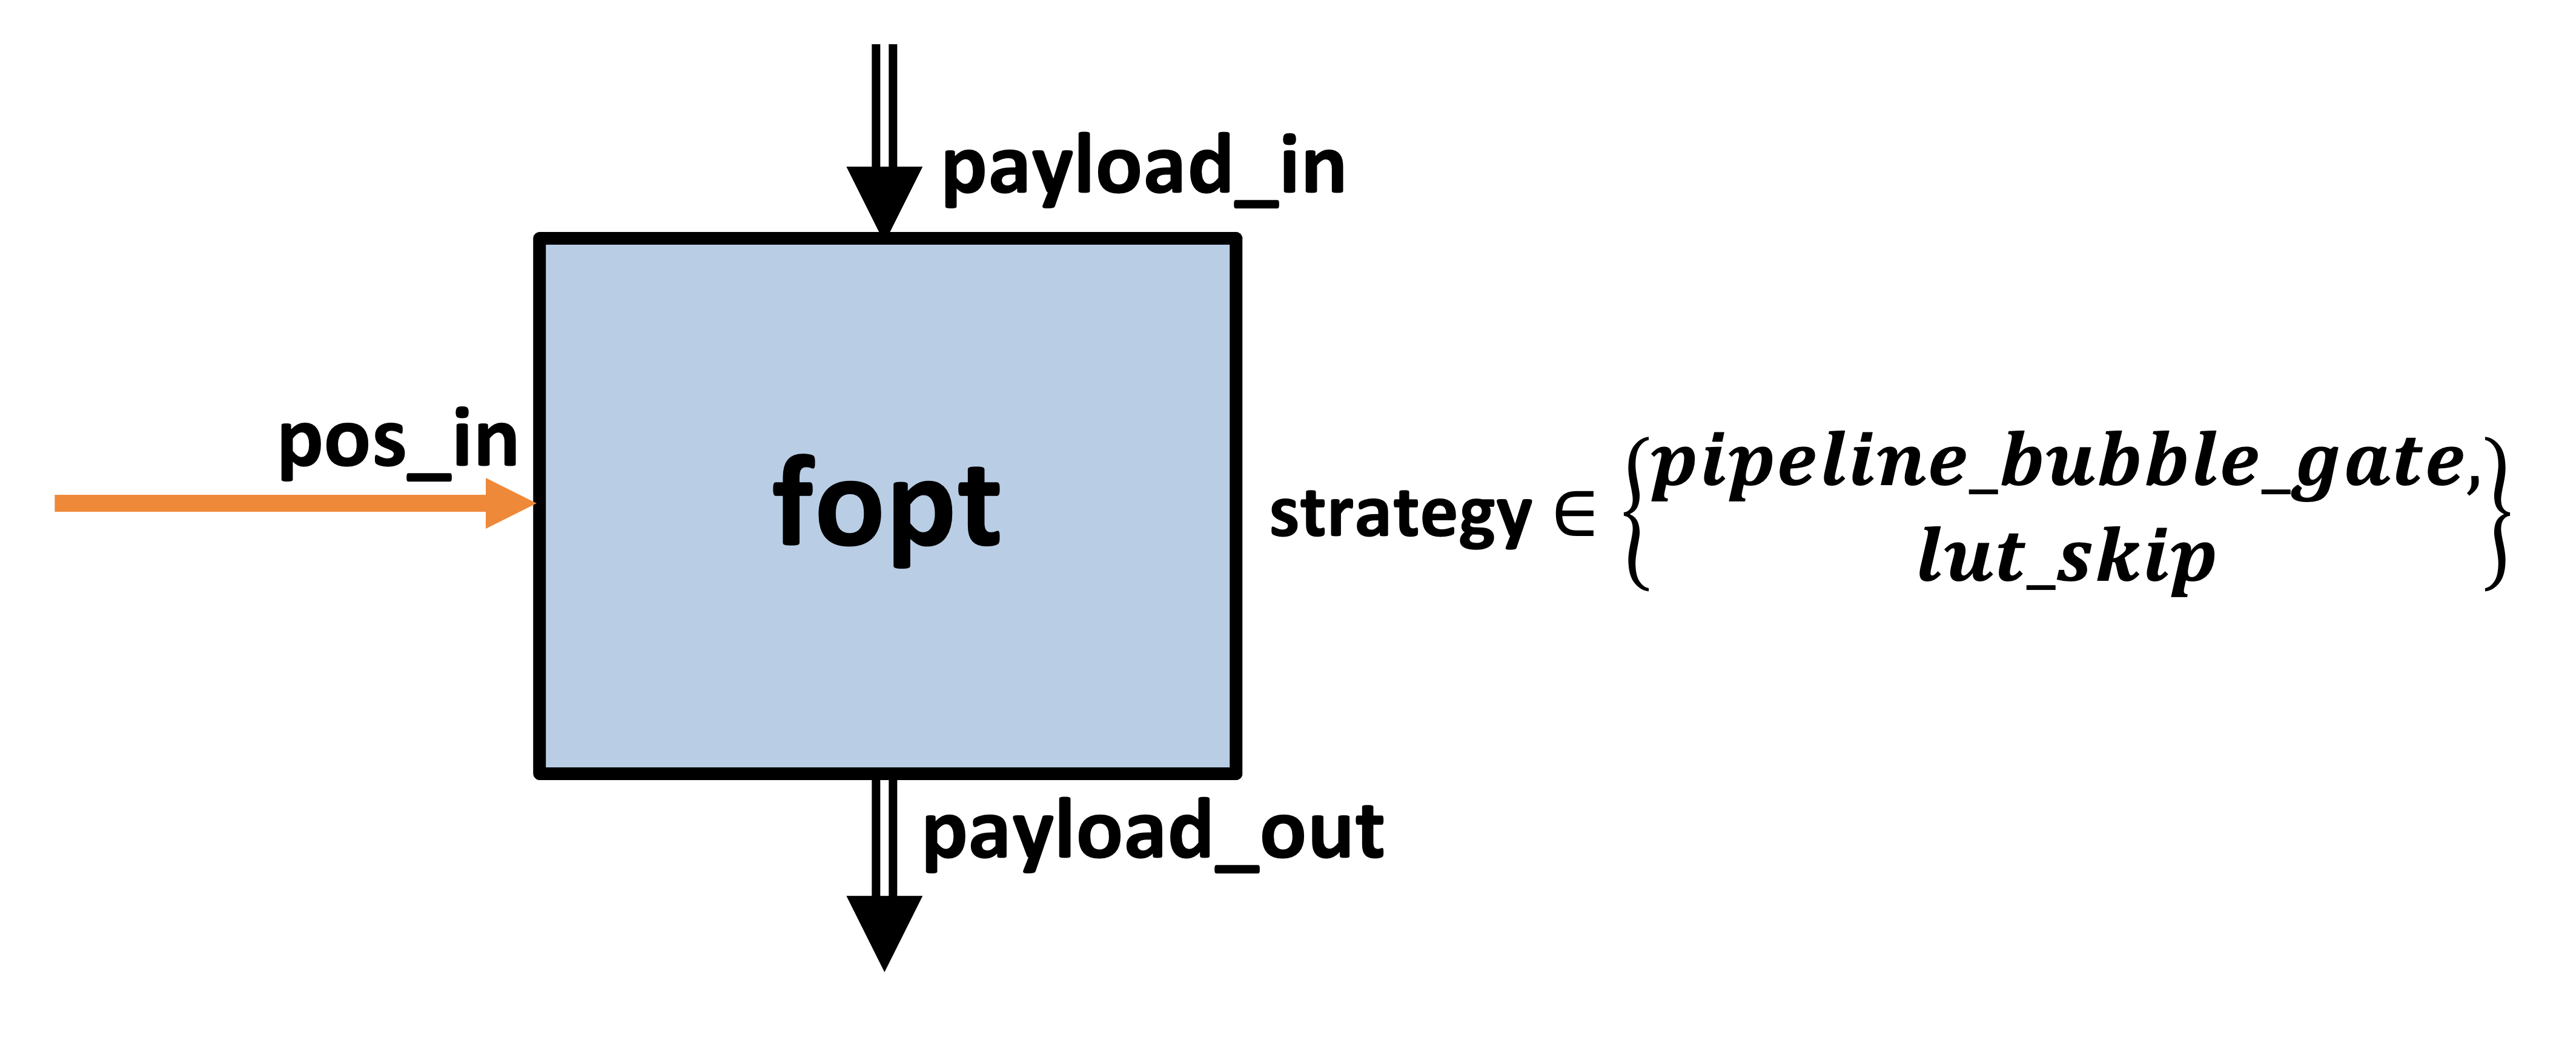
\includegraphics[width=0.95\textwidth]{figures/fopt.png}
    \caption{Fill optimizer primitive component template. }
    \label{fig:fopt}
\end{figure}

The attributes of a Fill optimizer are:

\begin{itemize}
    \item \textbf{strategy -} The fill optimization method.
    \begin{itemize}
    \item \textbf{pipeline\_bubble\_gate -} Eyeriss v2-style\cite{eyerissv2} strategy whereby unpaired leader payloads are discarded via pipeline bubble; depending on the amount of latency hiding facilitated by the pipelining, this may behave in a more gating-like or more skipping-like fashion.
    \item \textbf{lut\_skip -} GAMMA-style\cite{gamma} strategy whereby leader payloads are stored in a LUT and random-accessed by follower operand metadata. This implicitly discards unpaired leader operands.
    \end{itemize}
\end{itemize}

The supported customizations of Fill optimizer are shown in Table~\ref{tab:FillOptimizer_specializations}.

\begin{table}[H]
\centering
\begin{tabular}{l}
\toprule
 strategy             \\
\midrule
 pipeline\_bubble\_gate \\
 lut\_skip             \\
\bottomrule
\end{tabular}
\caption{Specializations of fill optimizer}
\label{tab:FillOptimizer_specializations}
\end{table}
\chapter{SAF microarchitecture taxonomy}
\label{chapter:saf_microarchitectures}

\section{SAF microarchitectures}
\label{chapter:saf_microarchitectures_section}

This section will overview the taxonomy of SAF microarchitectures considered in this work. SAF microarchitectures implement SAFs. Though not a requirement, in practice all SAF microarchitectures considered in this work were well-described as compound components, and conversely the only compound components modeled in this work happen to be SAF microarchitectures.

\subsection{Format microarchitectures}

\begin{figure}[H]
    \centering
    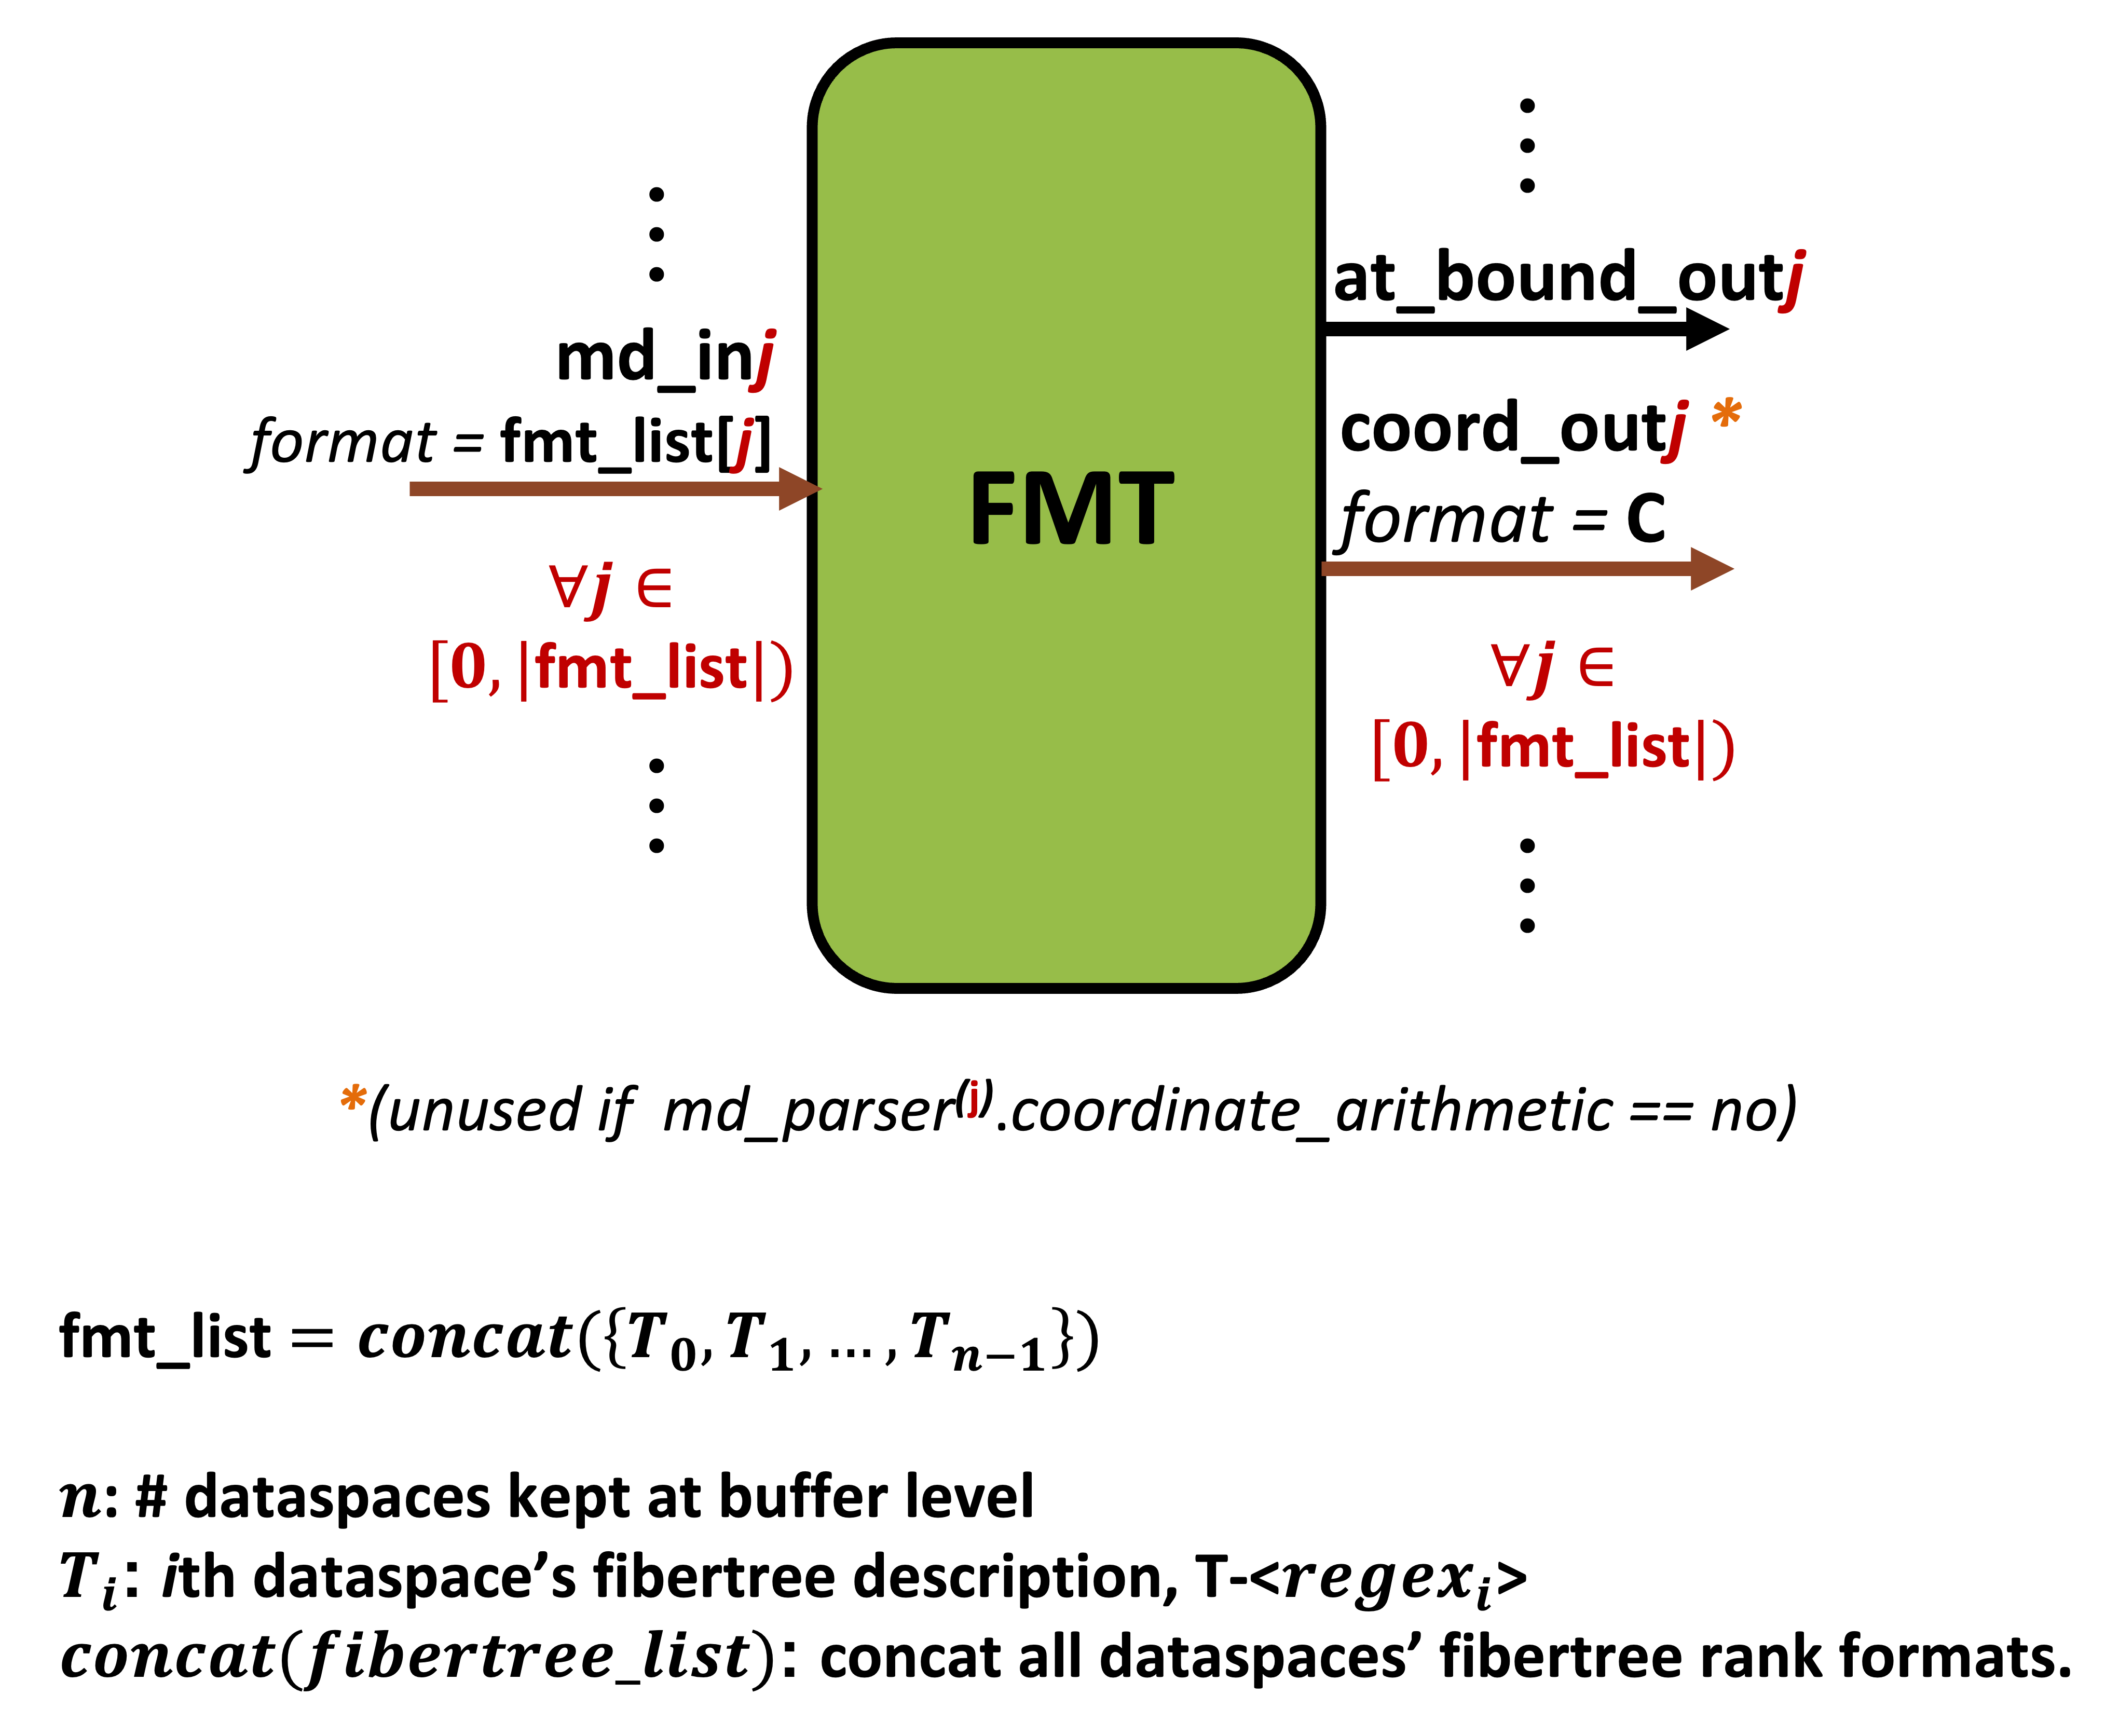
\includegraphics[width=0.95\textwidth]{figures/FMT.png}
    \caption{Format microarchitecture compound component template. If an architectural buffer has a format SAF, a format microarchitecture must be bound to it. The fmt\_list parameter expects a list of rank formats. The architectural buffer keeps\cite{timeloop} one or more dataspaces\cite{timeloop}, at least one of which exploits a format SAF. fmt\_list is assumed to have been derived from concatenating the fiber representation regexes\cite{szebook} for all kept dataspaces' fibertrees, excluding dataspaces which do not exploit a format SAF.}
    \label{fig:FMT}
\end{figure}

%\begin{table}[H]
%\centering
%\begin{tabular}{l}
%\toprule
% fibertree   \\
%\midrule
% *           \\
%\bottomrule
%\end{tabular}
%\caption{Specializations of format microarchitecture}
%\label{tab:format_microarchitecture_specializations}
%\end{table}

\begin{figure}[H]
    \centering
    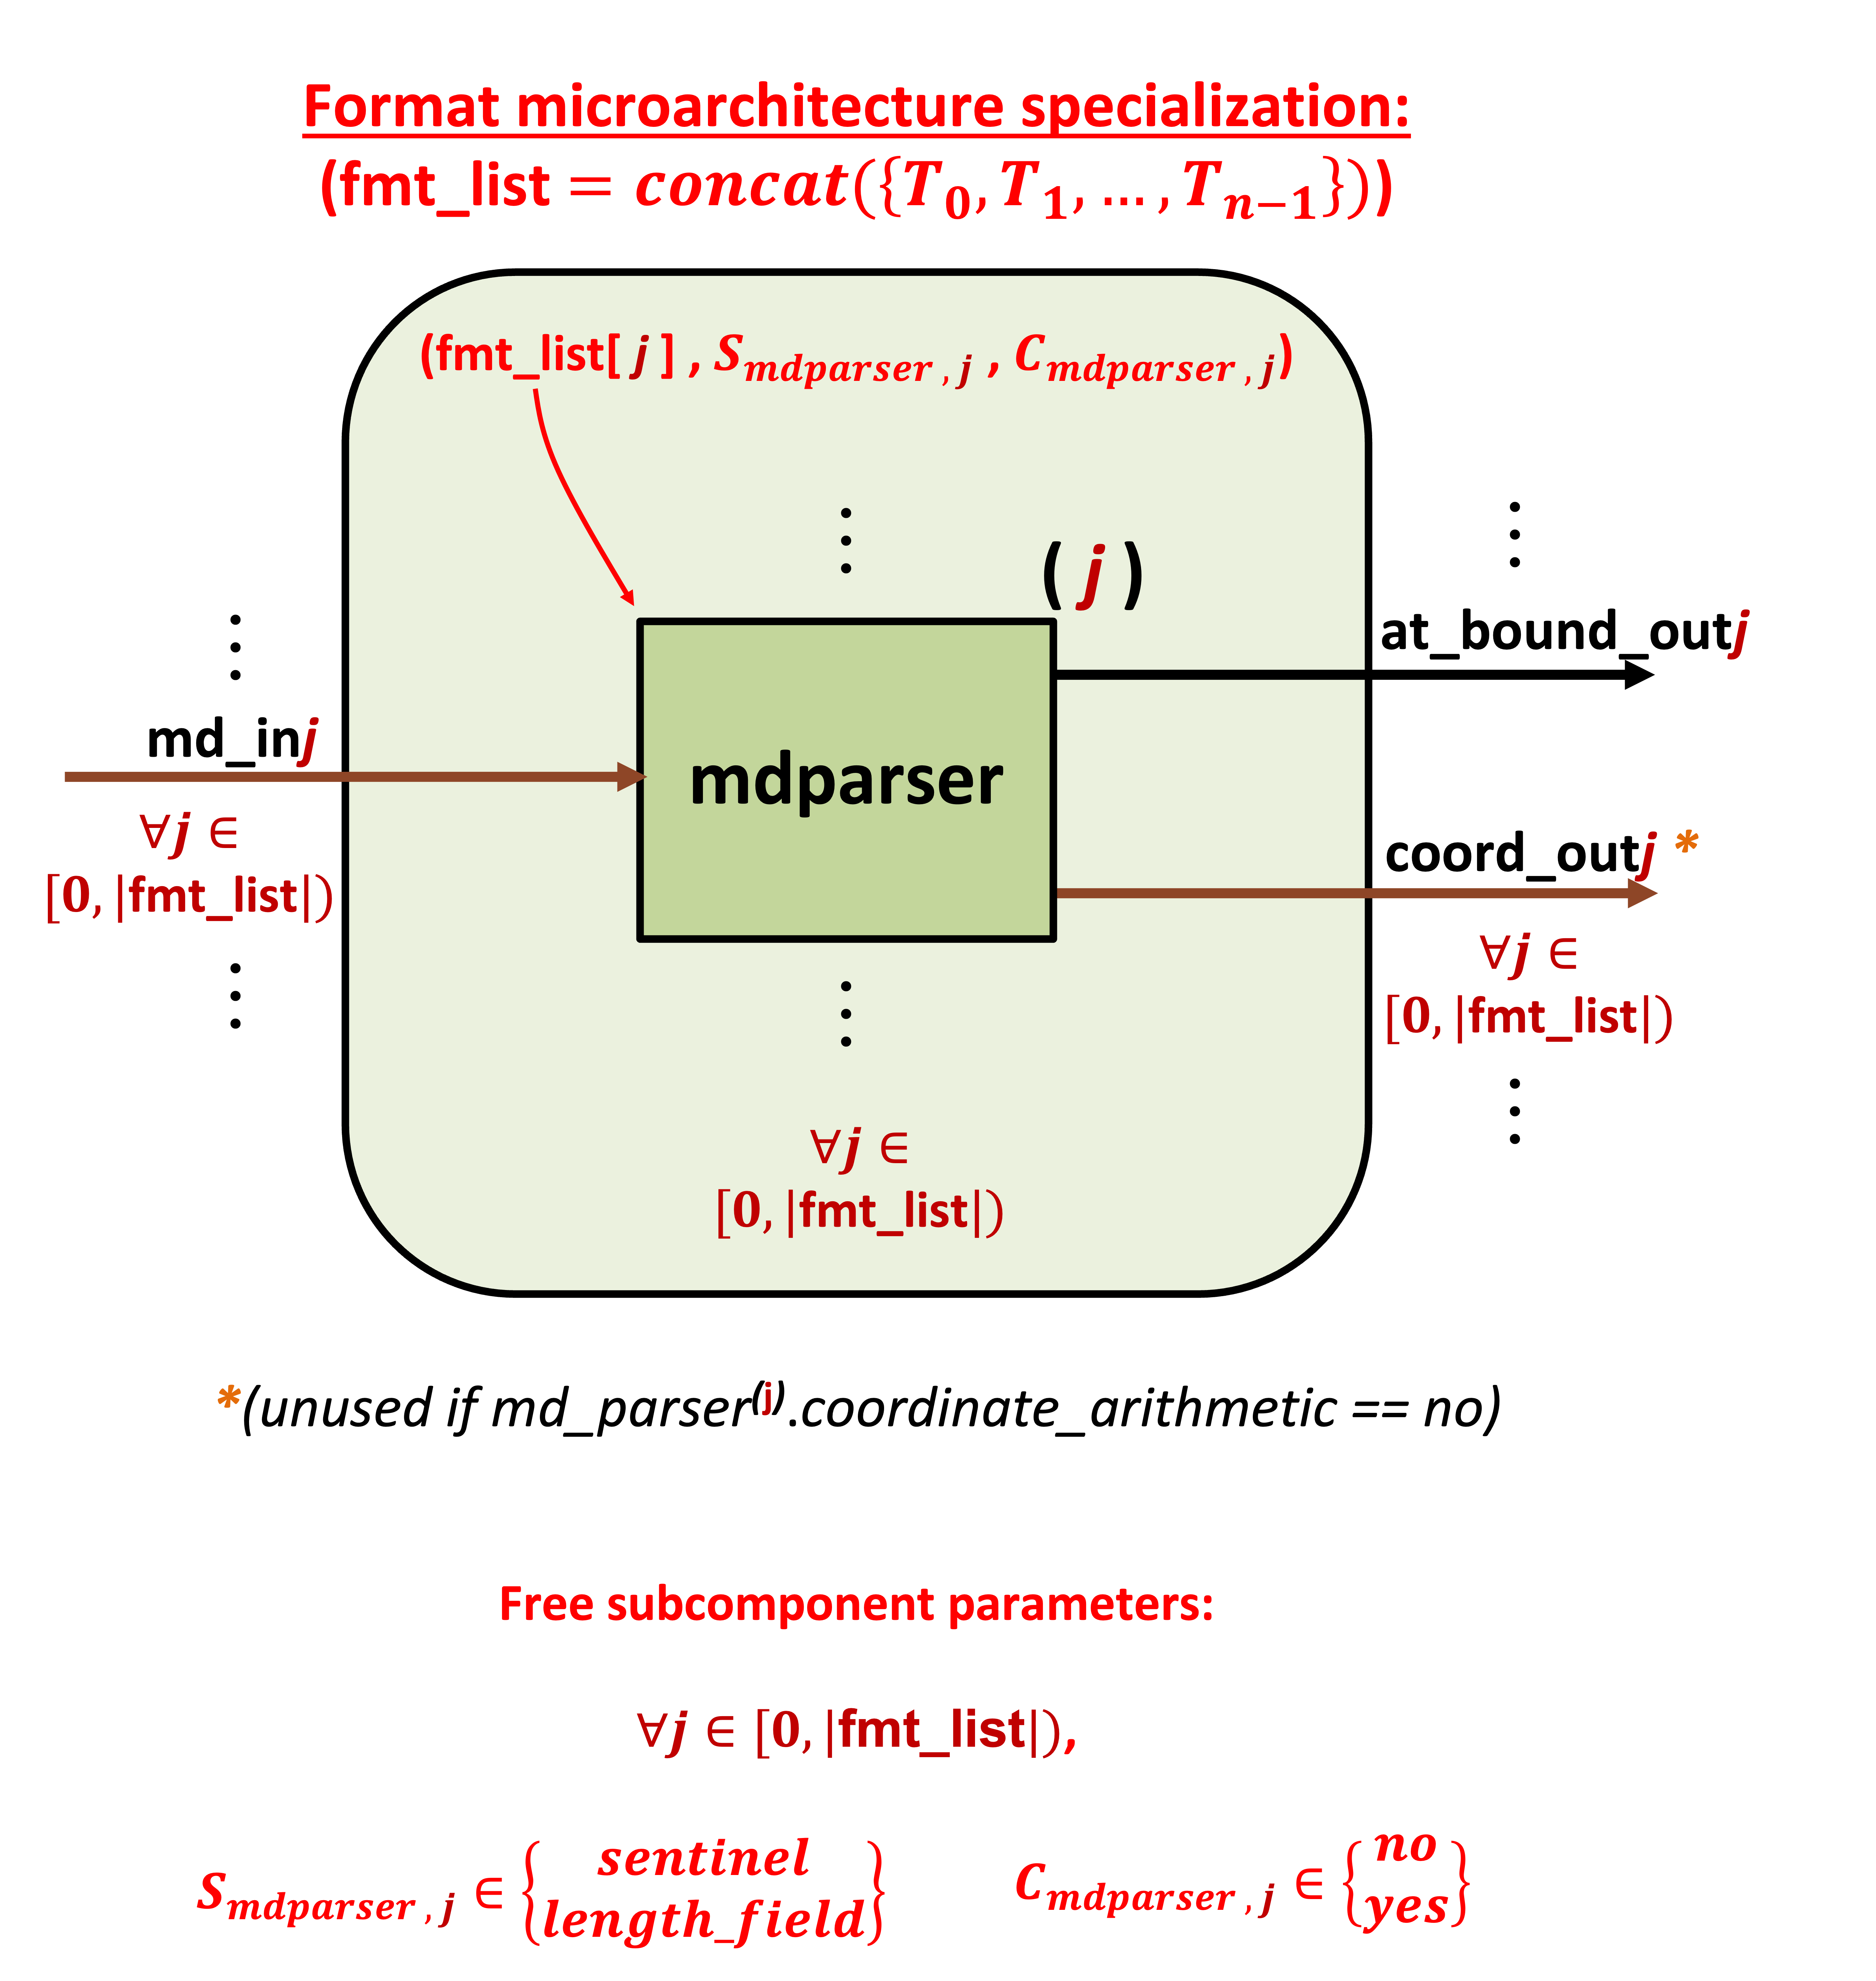
\includegraphics[width=0.95\textwidth]{figures/FMT_all.png}
    \caption{Format microarchitecture implementation topology. Every rank, in every fibertree, in every kept dataspace which is subject to a format SAF for a given buffer, has a corresponding metadata parser in the format microarchitecture topology. This implementation topology is universal for format microarchitectures regardless of the specific \textit{fmt\_list} parameter value. Each metadata parser subcomponent, however, has two free parameters. Setting \textit{coordinate\_arithmetic = no} for the $j$th metadata parser, means that that format microarchitecture will not support coordinate arithmetic for the corresponding fibertree rank. This can conserve resources i.e. if the rank is being contracted anyway.}
    \label{fig:FMT_all}
\end{figure}

\subsection{Skipping microarchitectures}

\begin{figure}[H]
    \centering
    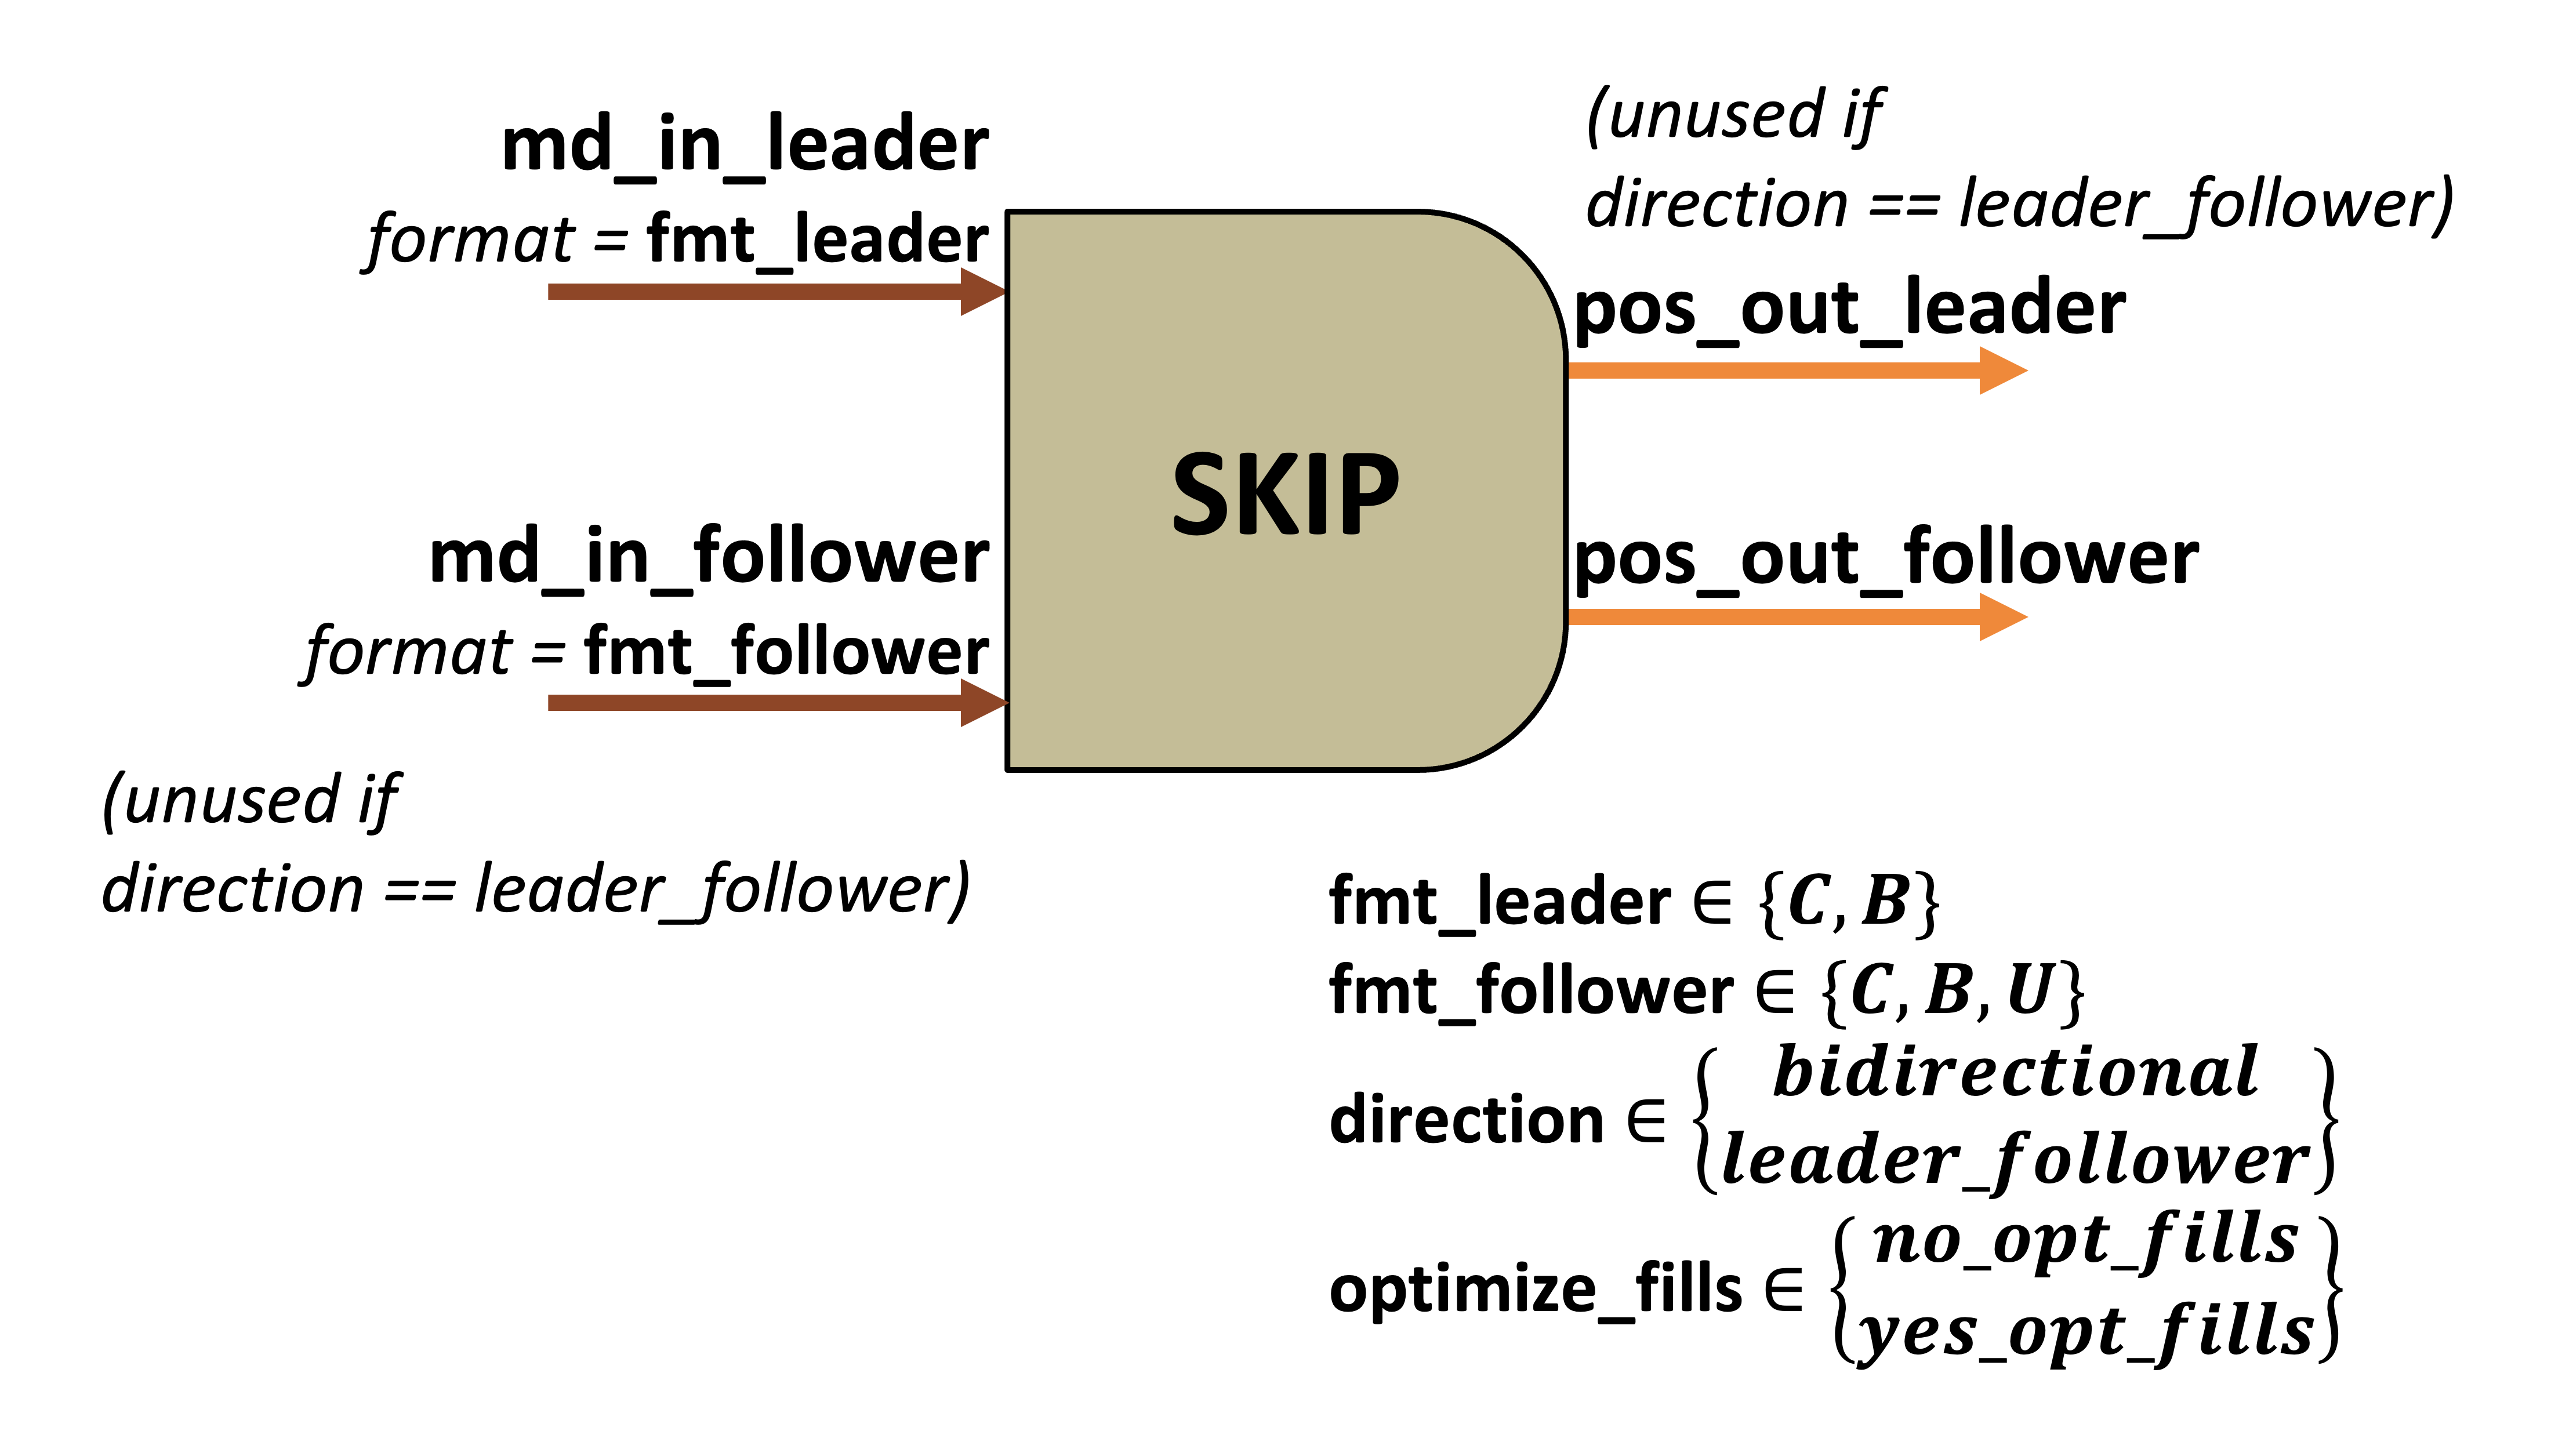
\includegraphics[width=0.95\textwidth]{figures/SKIP.png}
    \caption{Skipping microarchitecture compound component template.}
    \label{fig:SKIP}
\end{figure}

\subsubsection{Skipping microarchitecture specializations}

\begin{table}[ht]
\centering
\begin{tabular}{llll}
\toprule
 format\_leader   & format\_follower   & direction       & optimize\_fills   \\
\midrule
 C               & C                 & bidirectional   & no\_opt\_fills     \\
 B               & B                 & bidirectional   & no\_opt\_fills     \\
 C               & U                 & leader\_follower & no\_opt\_fills     \\
 C               & U                 & leader\_follower & yes\_opt\_fills    \\
\bottomrule
\end{tabular}
\caption{Specializations of skipping microarchitecture}
\label{tab:Skipping microarchitecture_specializations}
\end{table}

\begin{figure}[H]
    \centering
    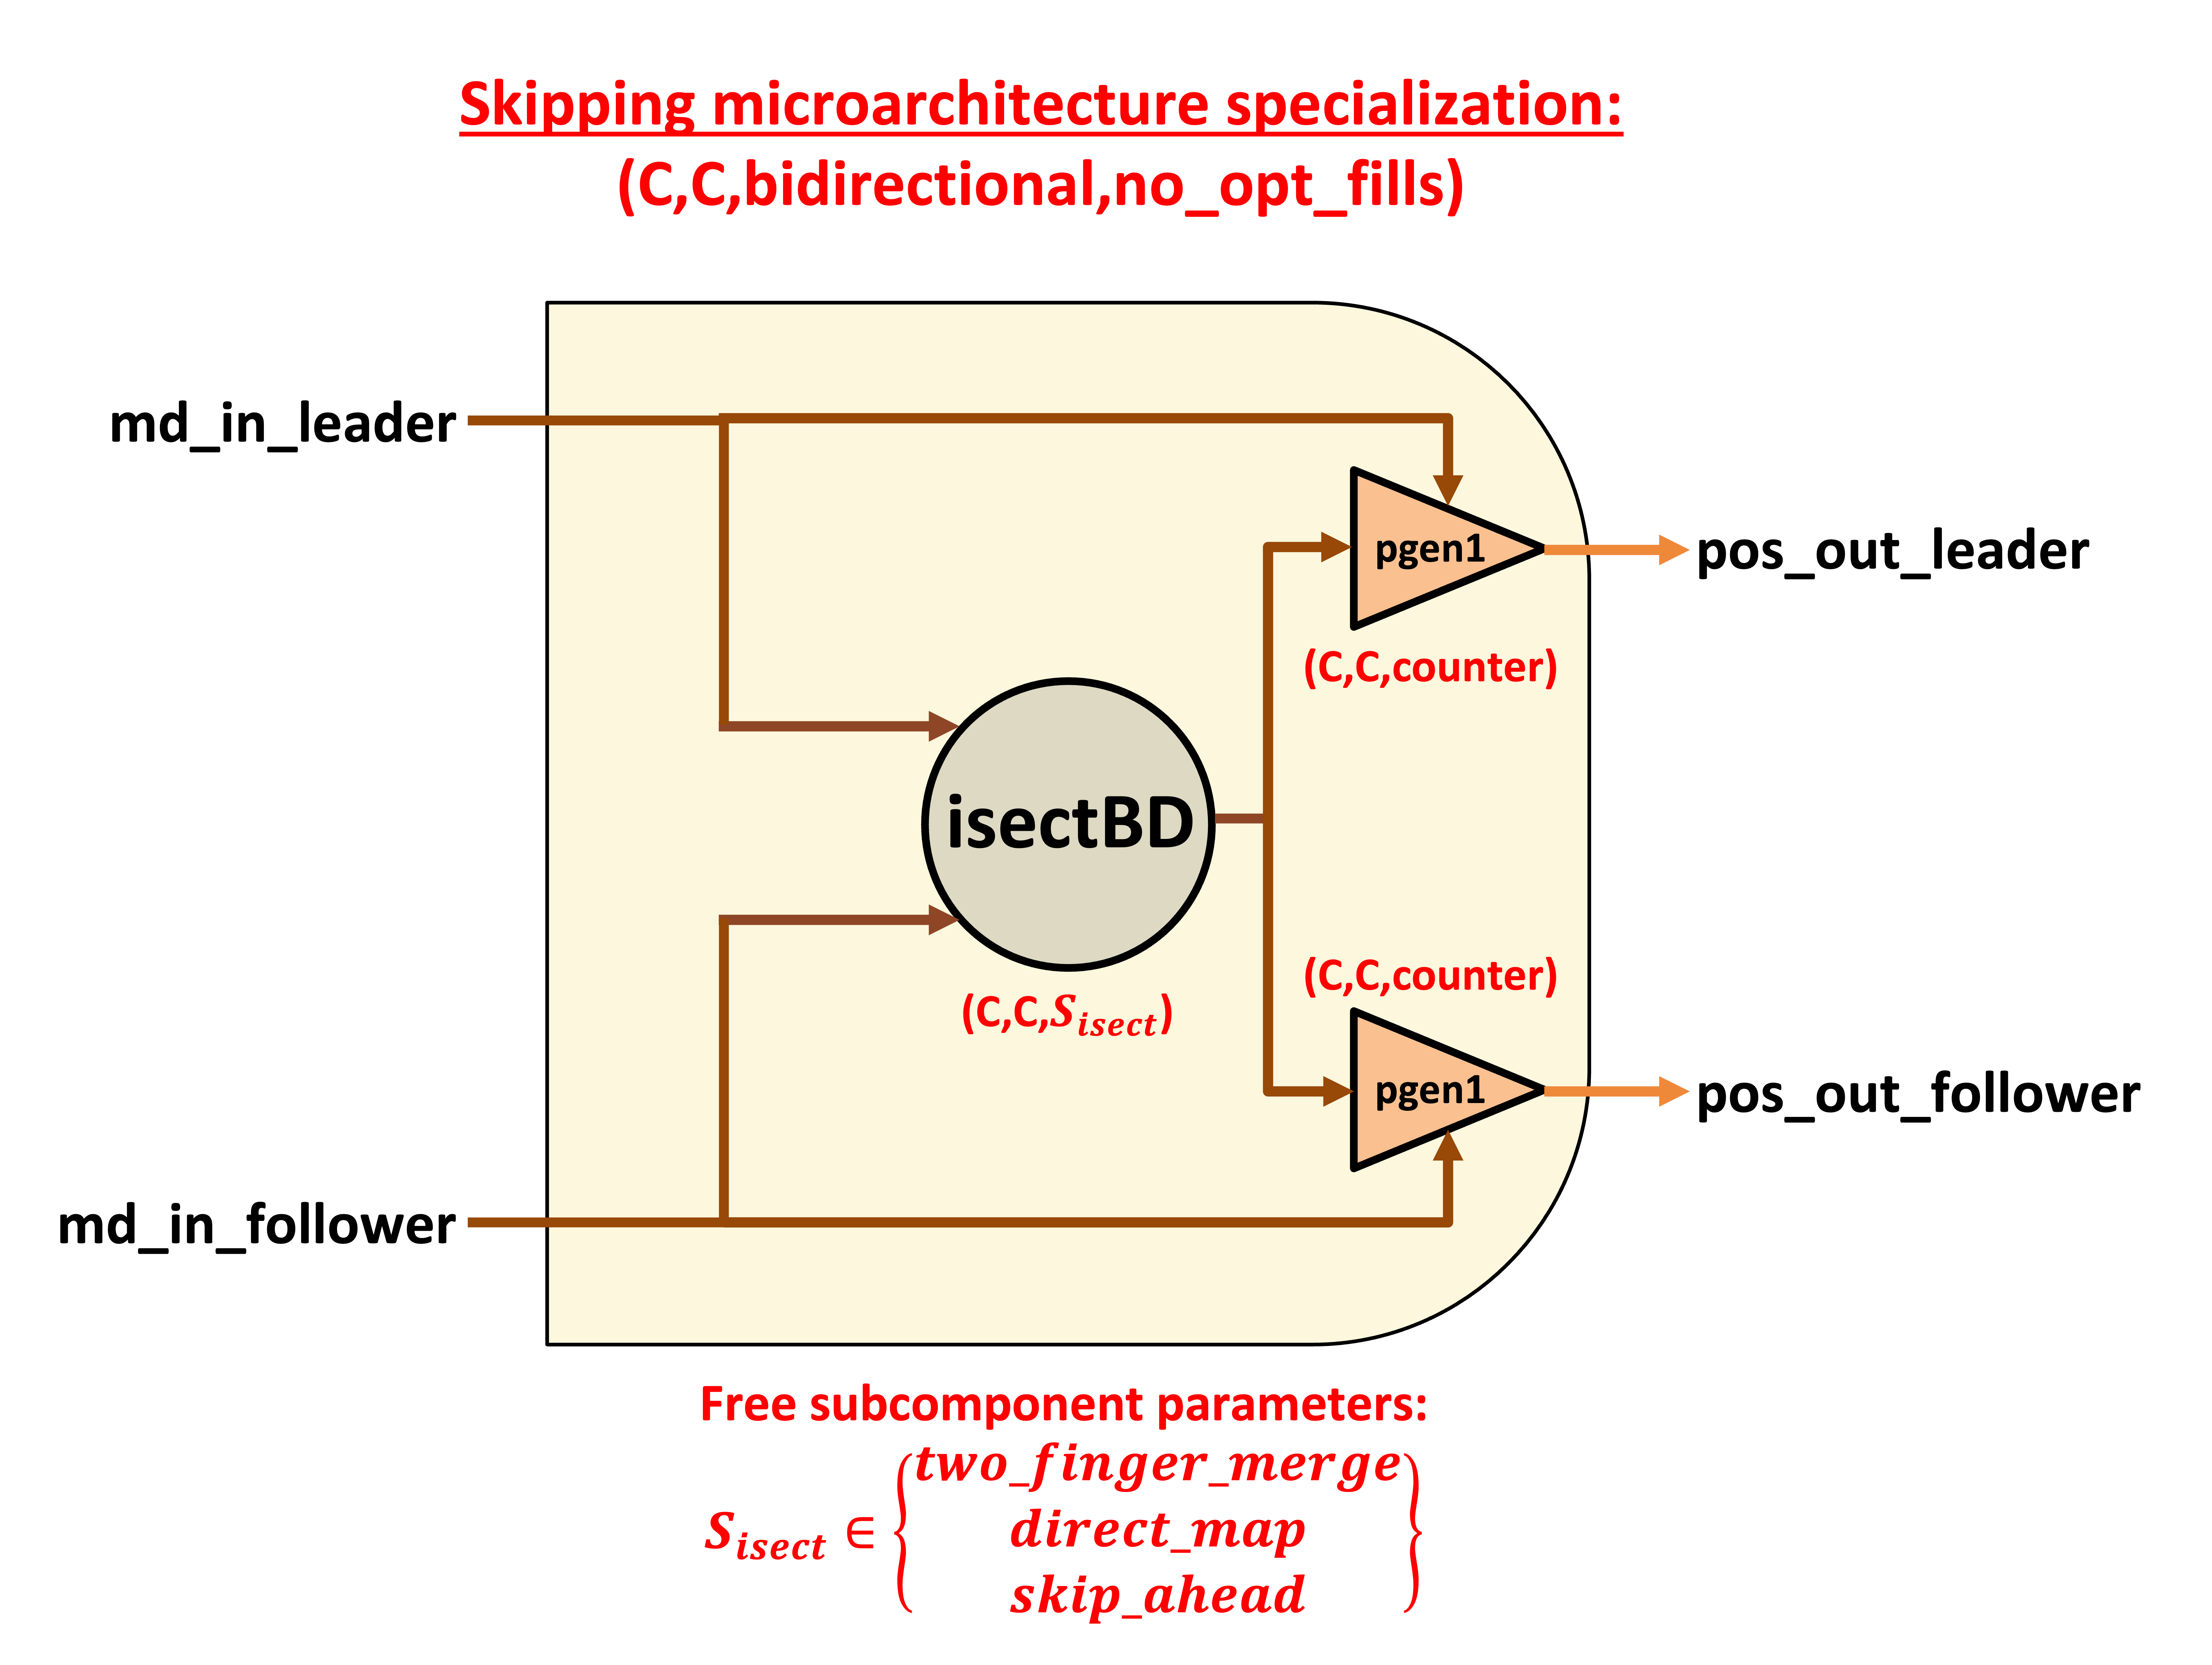
\includegraphics[width=0.95\textwidth]{figures/SKIP_C_C_bidirectional_no_opt_fills.png}
    \caption{Bidirectional coordinate-payload (C) skipping microarchitecture implementation topology (``ExTensor-like''\cite{extensor}.)}
    \label{fig:SKIP_C_C_bidirectional_no_opt_fills}
\end{figure}

\begin{figure}[H]
    \centering
    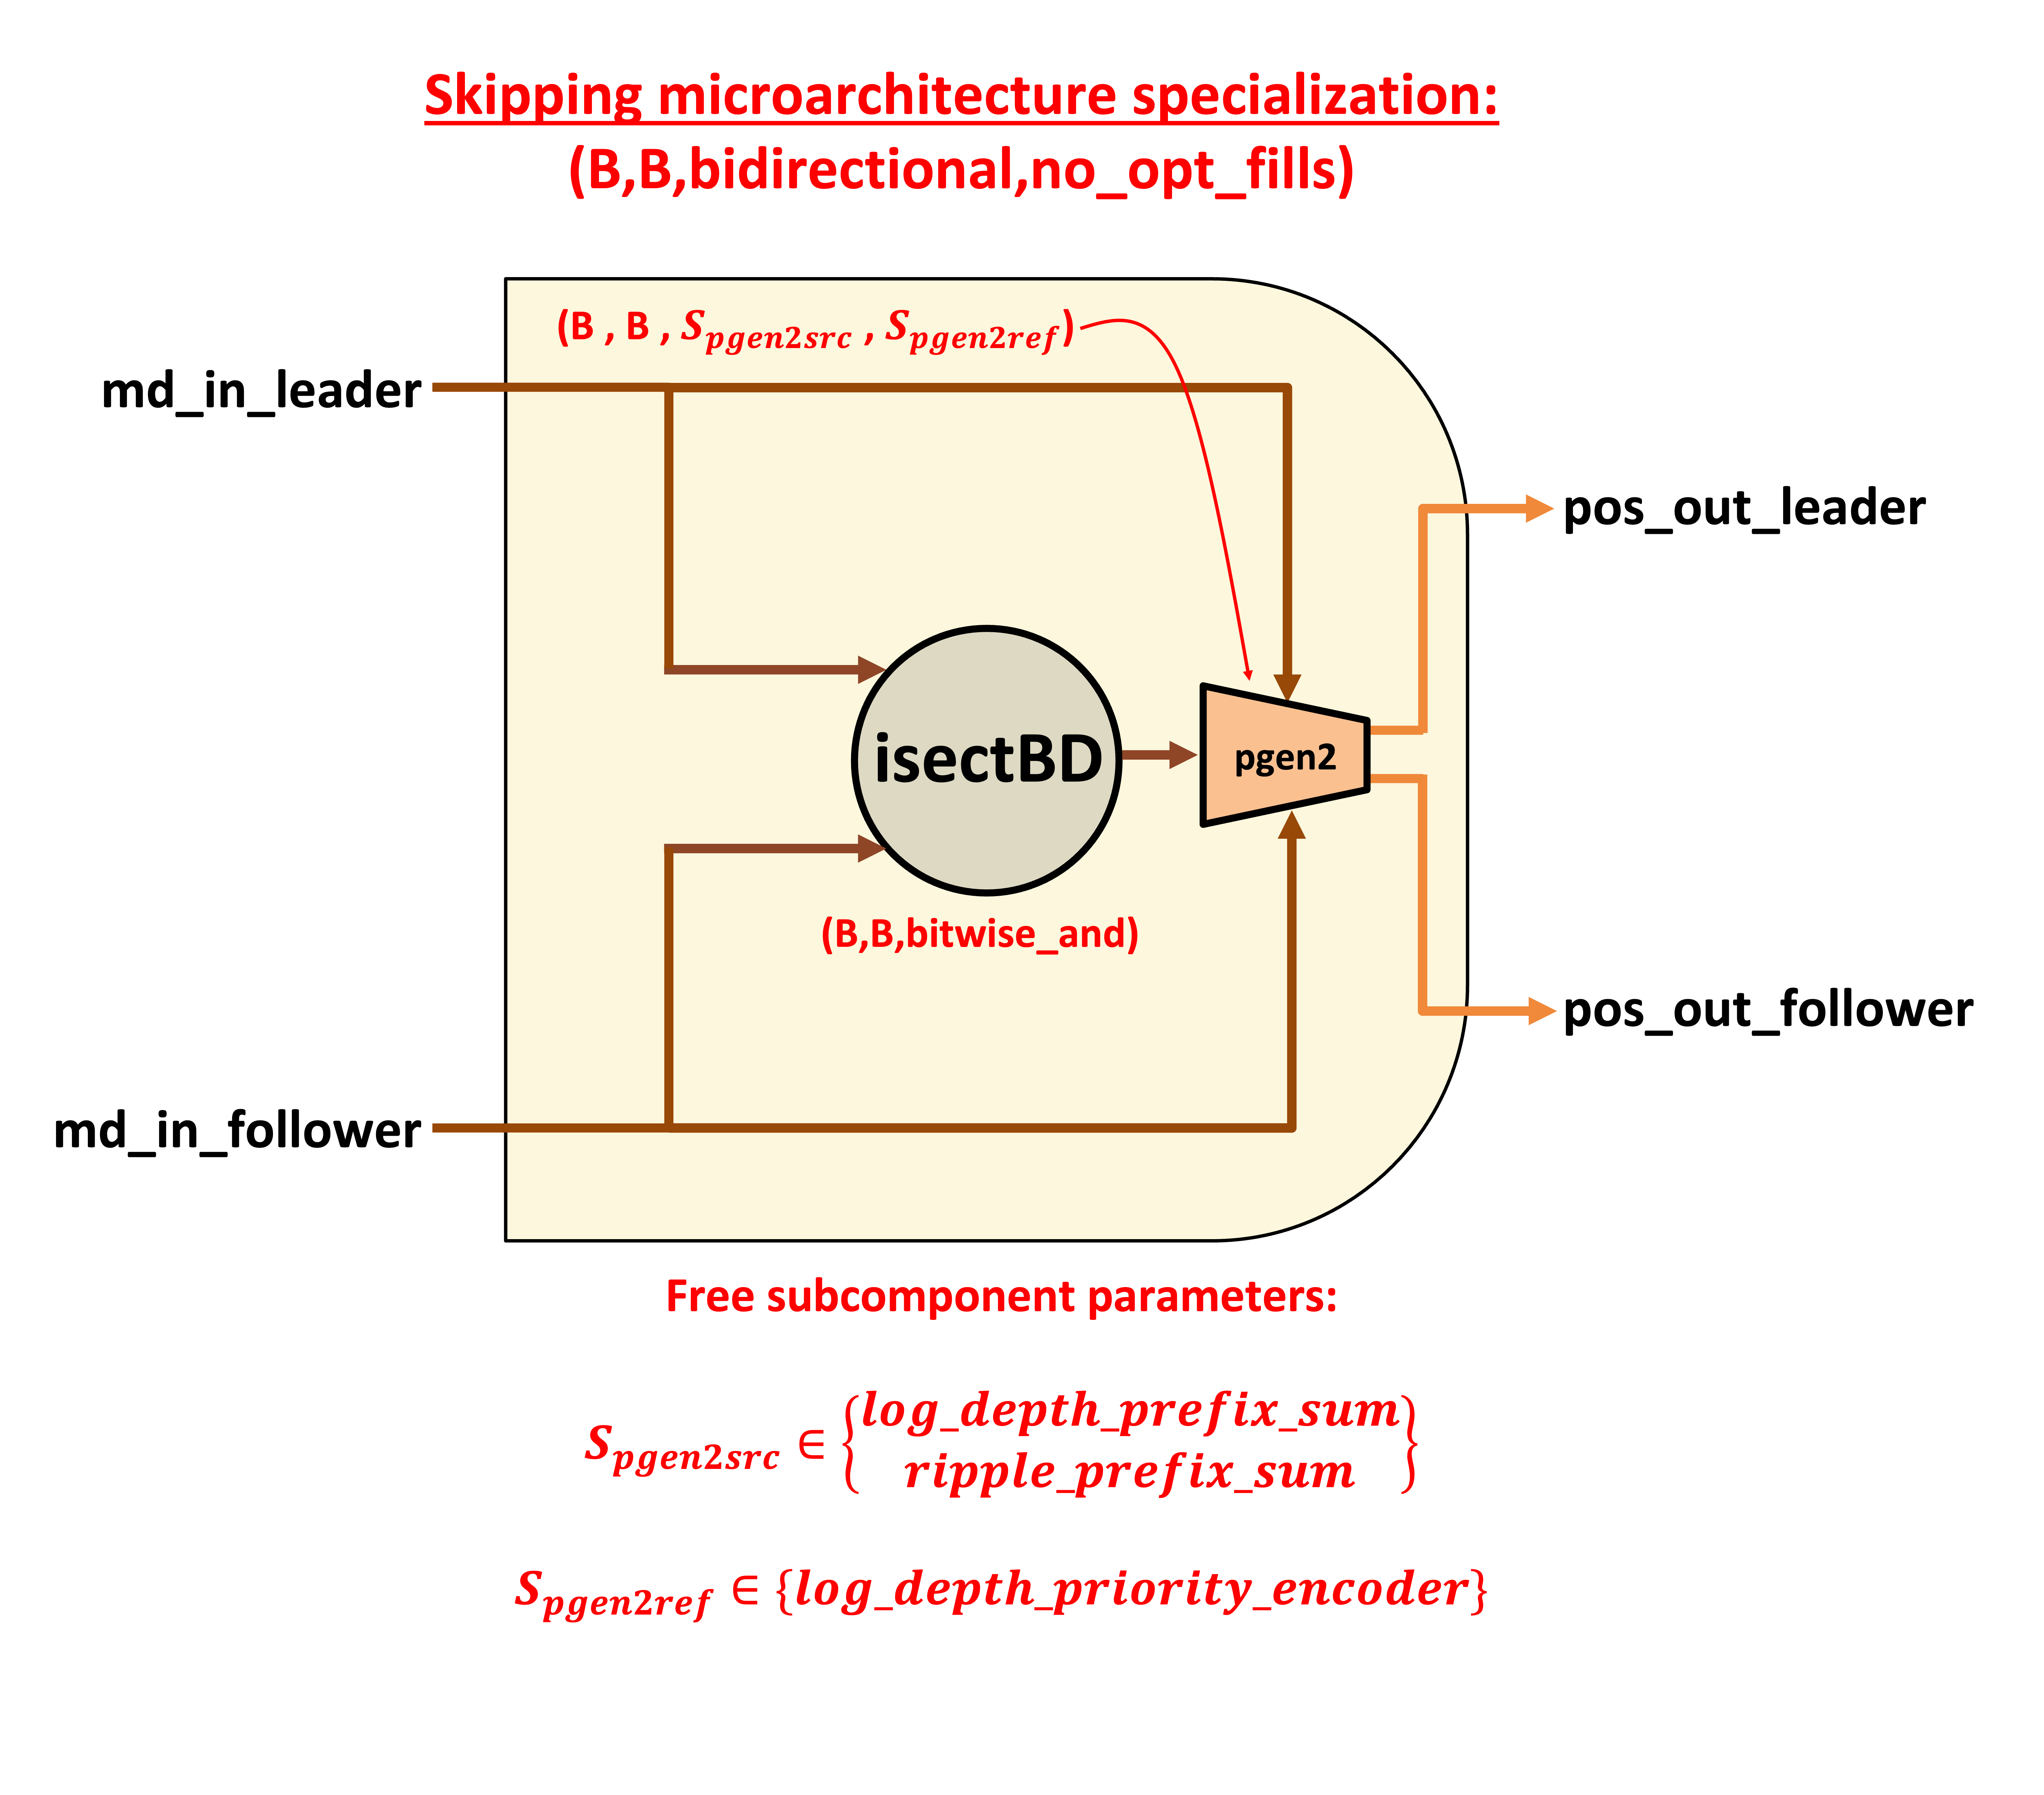
\includegraphics[width=0.95\textwidth]{figures/SKIP_B_B_bidirectional_no_opt_fills.png}
    \caption{Bidirectional bitmask (B) skipping microarchitecture implementation topology (``SparTen-like''\cite{sparten}.)}
    \label{fig:SKIP_B_B_bidirectional_no_opt_fills}
\end{figure}

\begin{figure}[H]
    \centering
    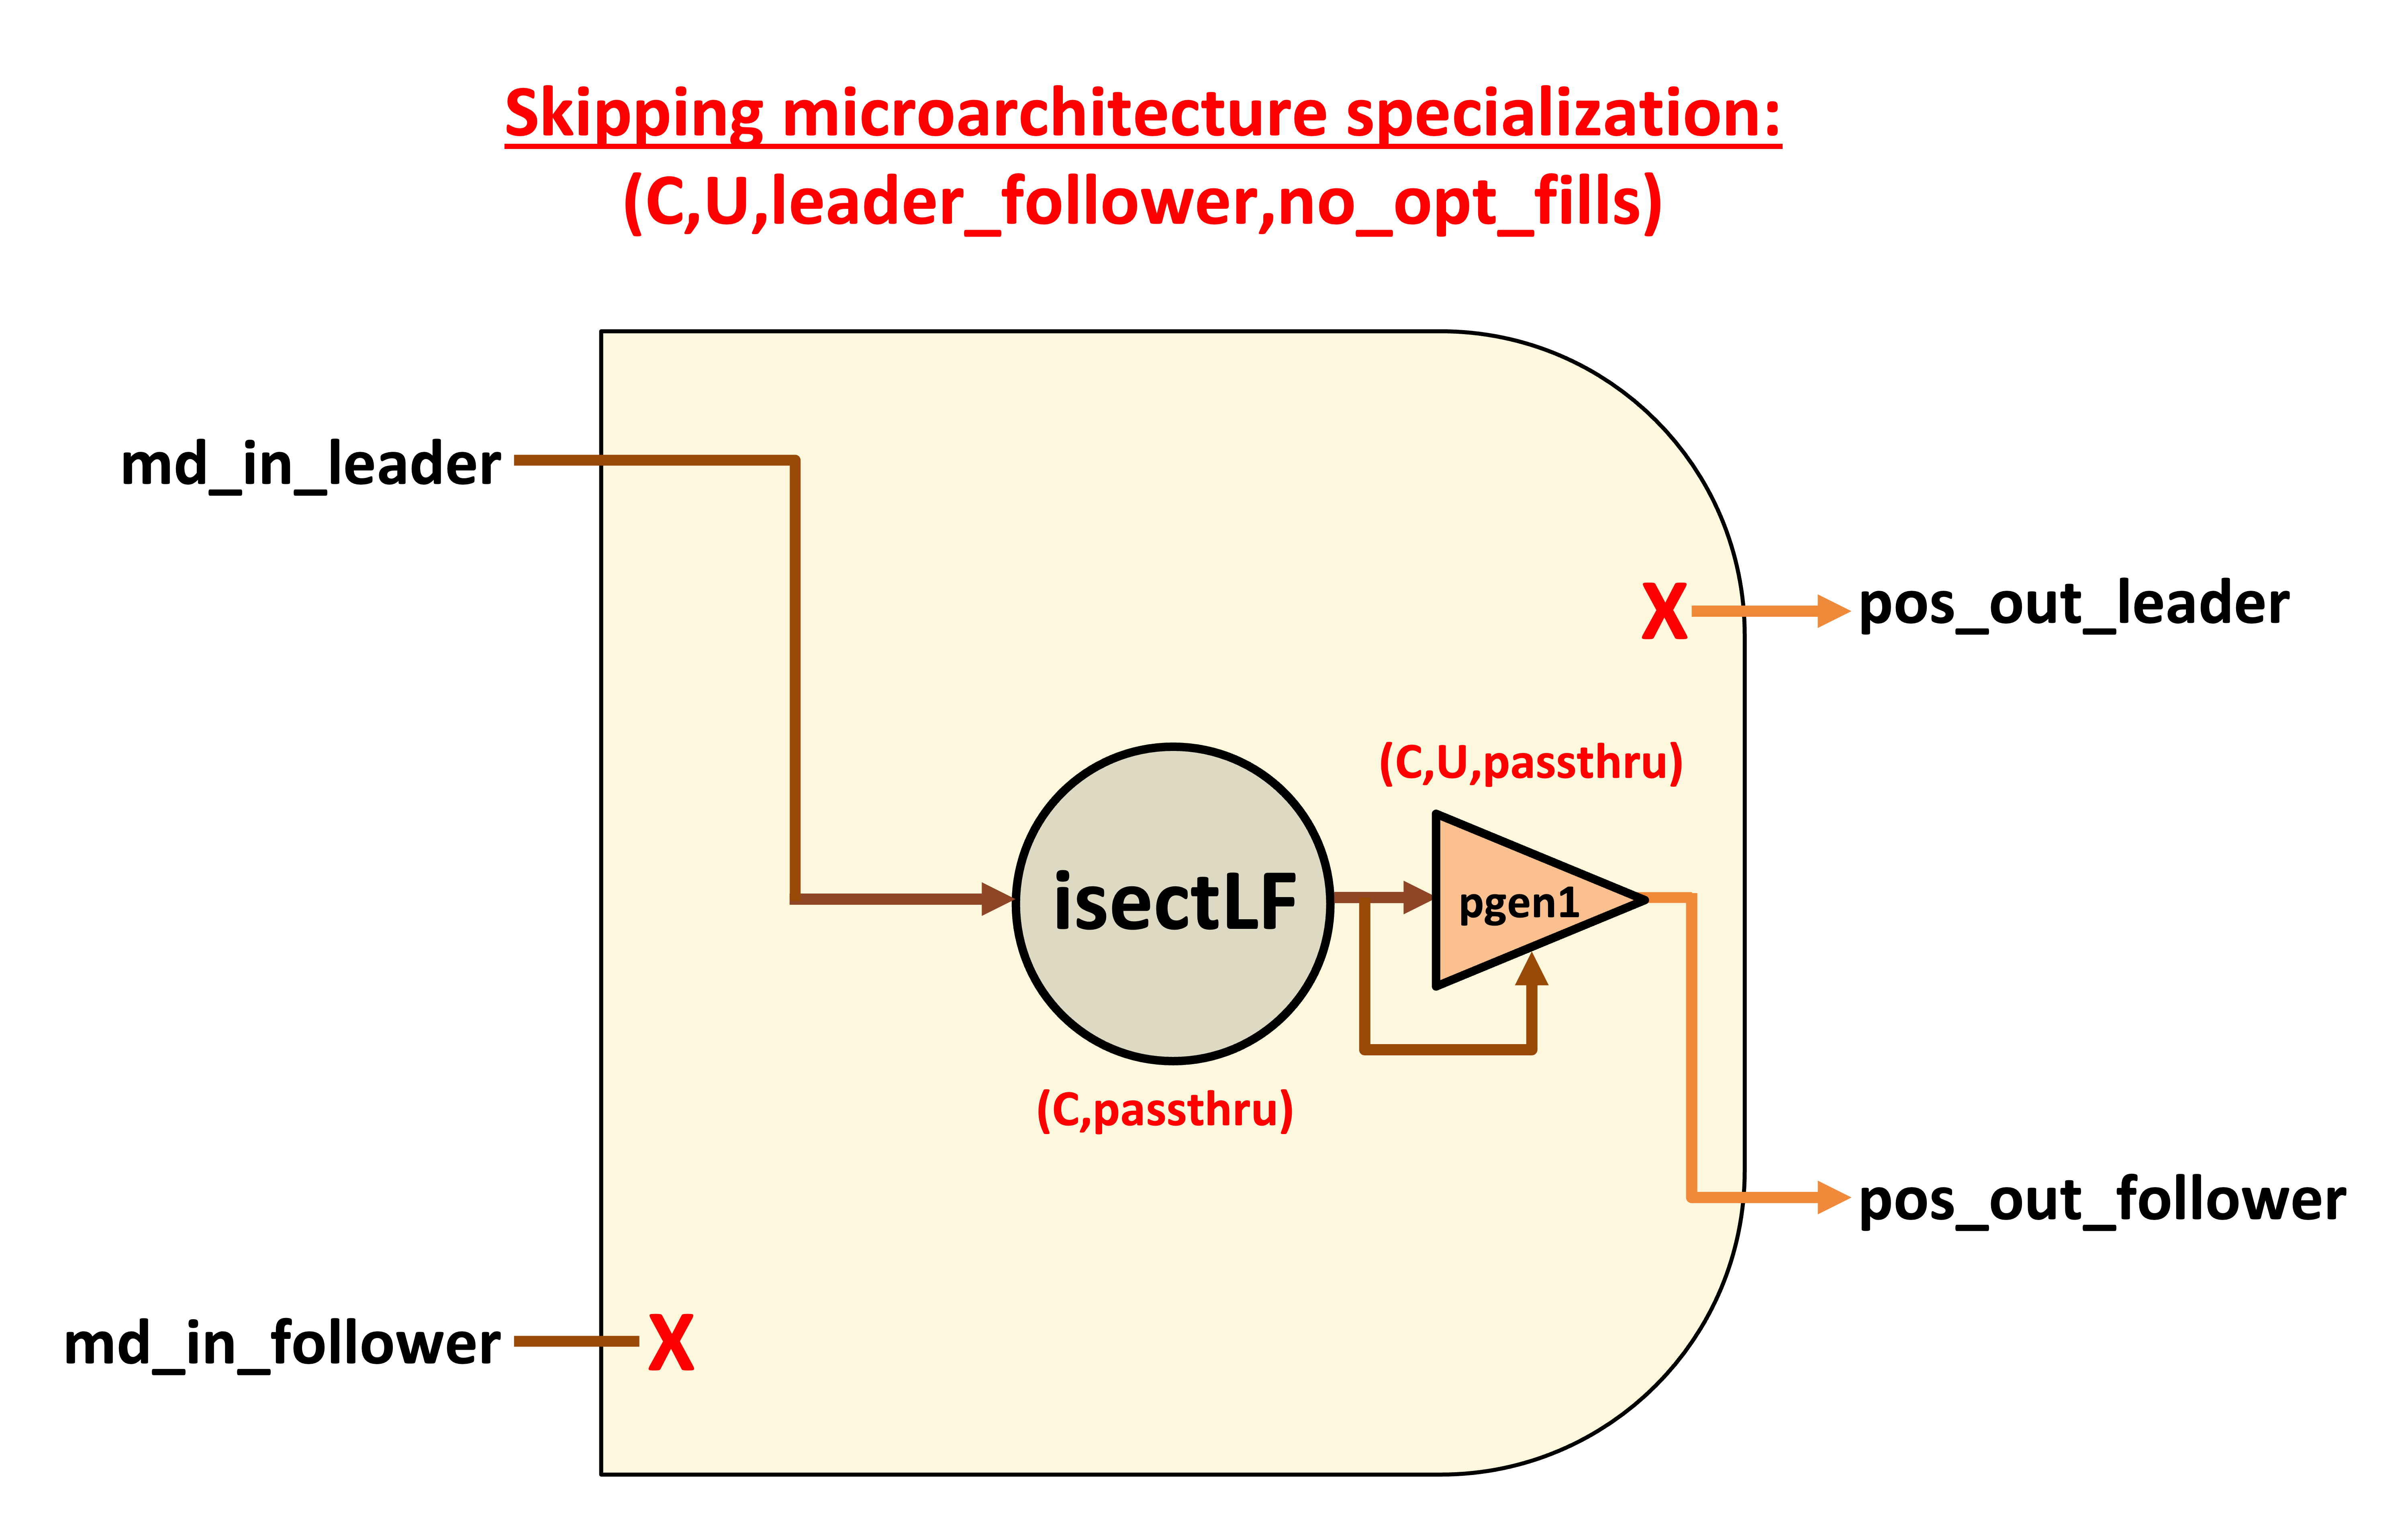
\includegraphics[width=0.95\textwidth]{figures/SKIP_C_U_leader_follower_no_opt_fills.png}
    \caption{Leader-follower coordinate-payload (C) to uncompressed offset-pair (U) skipping microarchitecture implementation topology, without fill optimization.}
    \label{fig:SKIP_C_U_leader_follower_no_opt_fills}
\end{figure}

\begin{figure}[H]
    \centering
    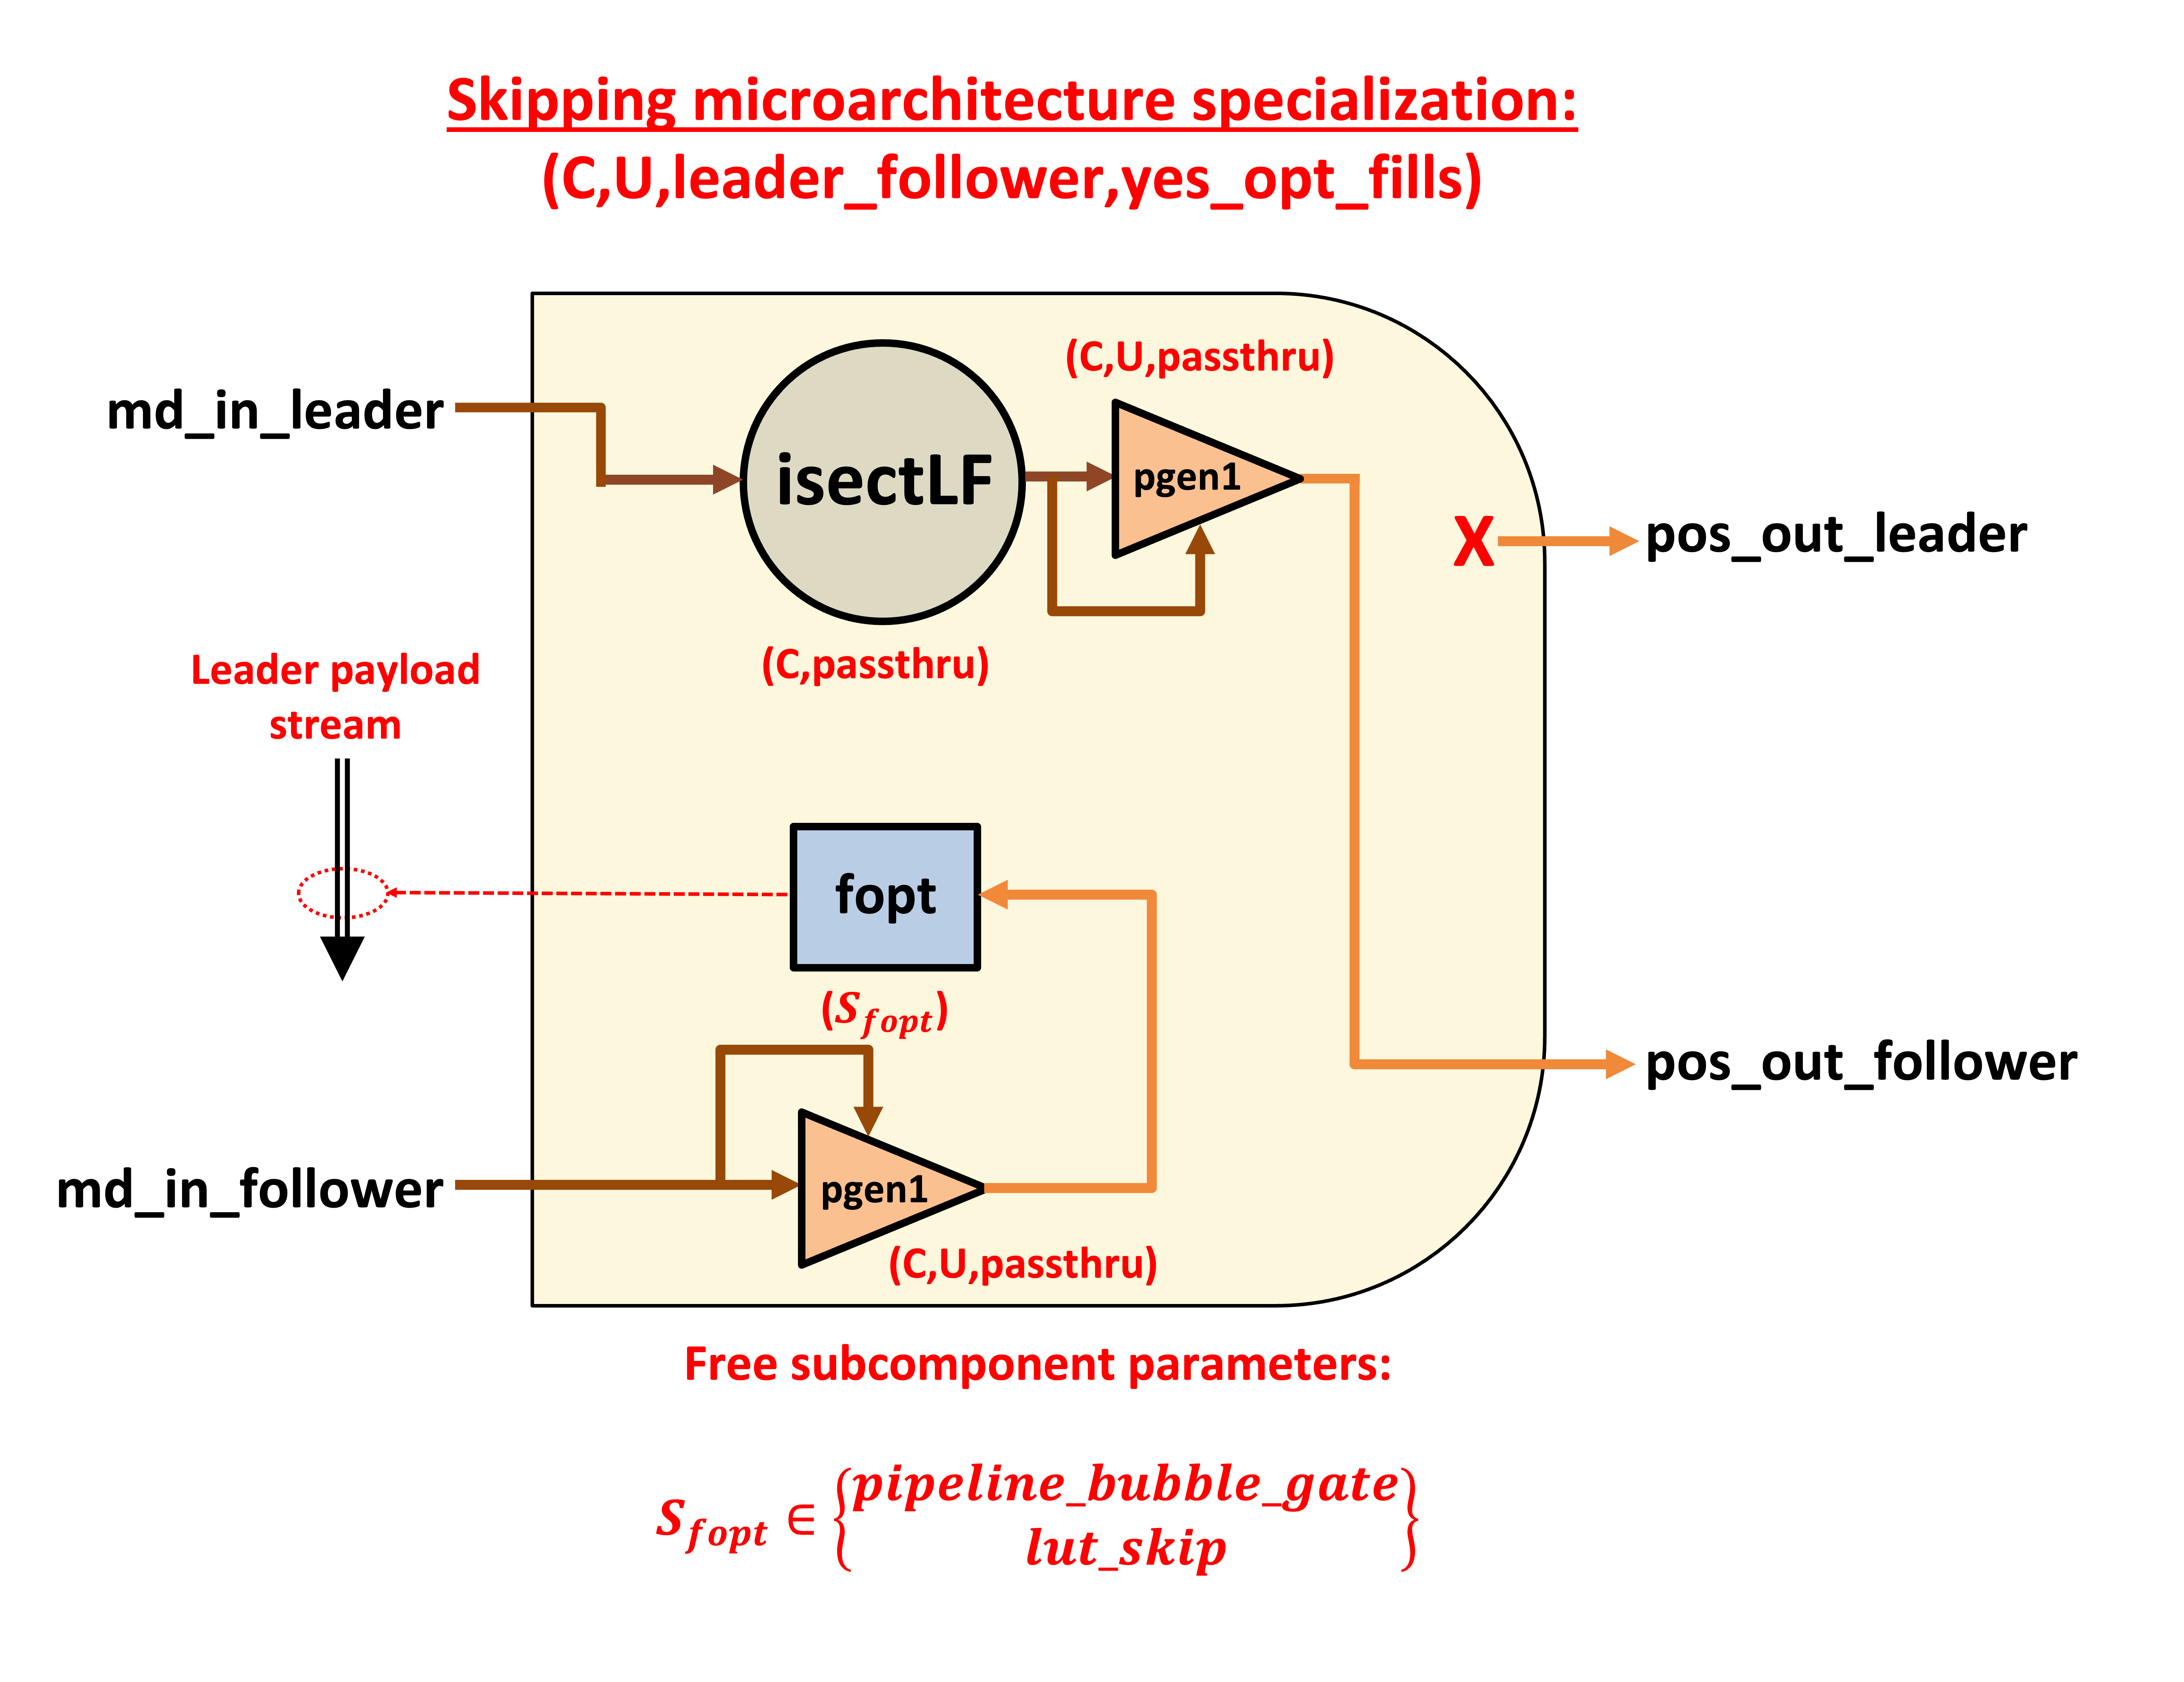
\includegraphics[width=0.95\textwidth]{figures/SKIP_C_U_leader_follower_yes_opt_fills.png}
    \caption{Leader-follower coordinate-payload (C) to uncompressed offset-pair (U) skipping microarchitecture implementation topology, with fill optimization (``Eyeriss-v2-like''\cite{eyerissv2}.)}
    \label{fig:SKIP_C_U_leader_follower_yes_opt_fills}
\end{figure}

\section{SAF concretization}
\label{chapter:saf_concretization}
\chapter{SAFtools framework}


\chapter{Evaluation}
\label{chapter:evaluation}

\section{Methodology}

\todo{Describe validation and evaluation process}

%\subsection{Simulation Speed}

\section{Validation}

\todo{Model PE experiment} 
\chapter{Case study}
\label{chapter:case_studies}

This case-study explores the tradeoff of different skipping microarchitectures in a scenario where the sparse tensor accelerator exploits a SIMD MAC.

\section{Methodology}

 Here one case study is provided which showcases

\begin{itemize}
    \item SAF microarchitecture taxonomic inference with SAFinfer.
    \item SAF microarchitecture scale inference with SAFmodel.
    \item Tradeoff study comparing different choices of coordinate-payload intersection unit.
\end{itemize}

SAFmodel was also used to generate Accelergy analytical models for use with Sparseloop; however, for a variety of reasons, these models were not integrated into a Sparseloop testbench; the tradeoff study here only compares the energy-per-action and area overhead of SAF microarchitectures but does not use Sparseloop to obtain action counts or get energy/area estimates for the rest of the architecture.

SAFTools allows the user to customize the objective function for optimizing SAF microarchitecture. In this work, the objective function is the total energy-per-action/area product, over all SAF microarchitecture primitives and all actions. This is the default SAFTools objective function, and it is chosen in order to co-optimize energy and area. 

\begin{figure}[ht]
\centering
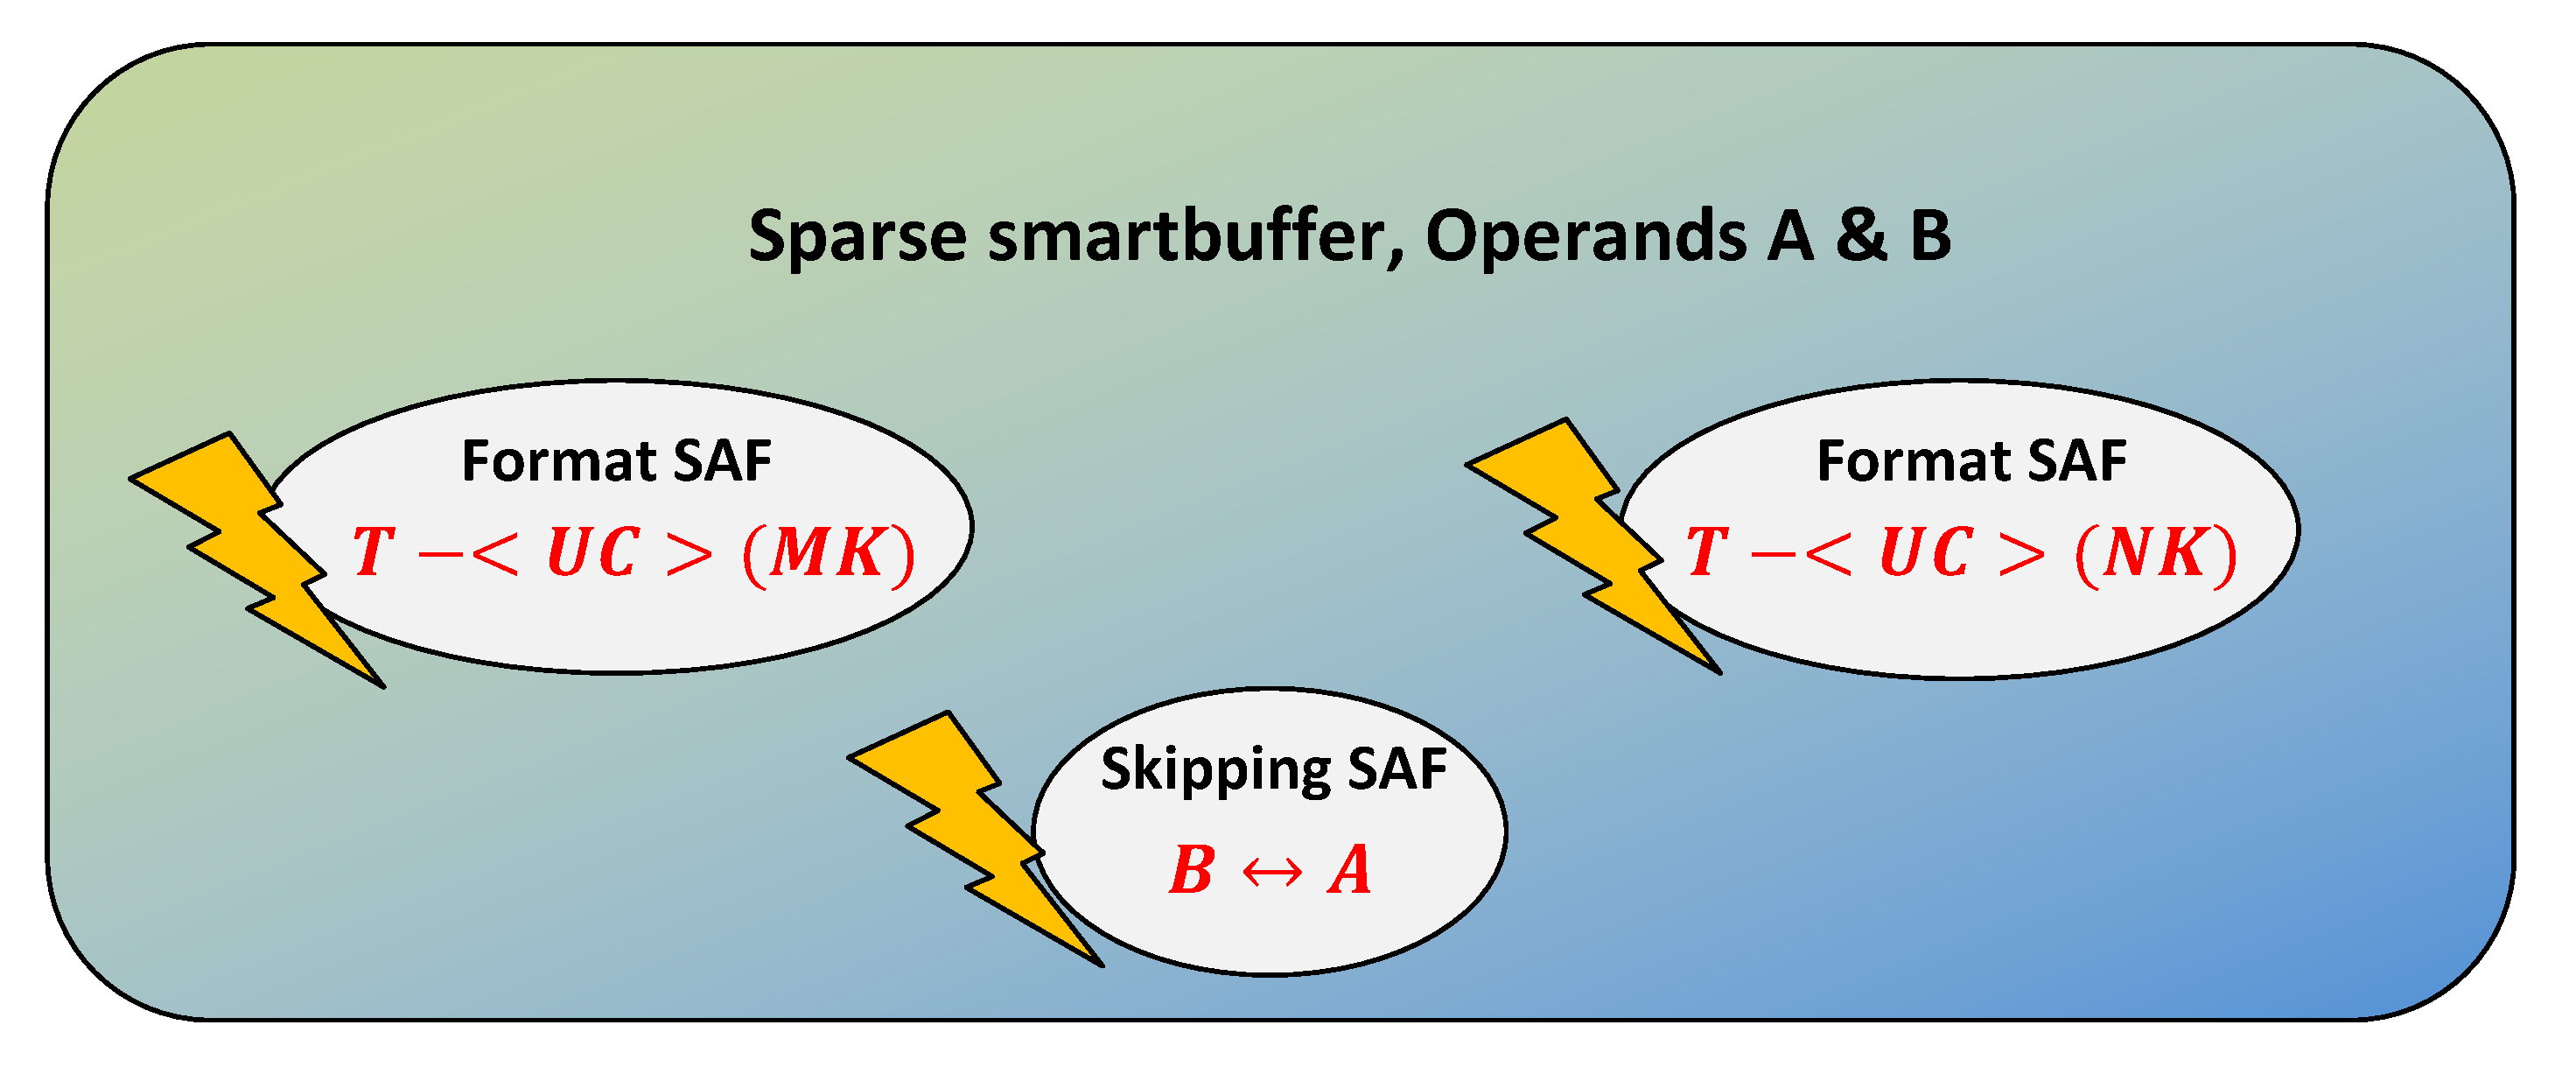
\includegraphics[width=0.85\textwidth]{figures/case_study_declarative.pdf}
\caption{Sparseloop configuration files provided to SAFinfer.}
\label{fig:case_study_declarative}
\end{figure}

For taxonomic inference, SAFinfer was provided Sparseloop configuration files specifying a hypothetical architecture with a buffer holding both input operands resident, both in CSR format (T-<UC>(MK) and T-<UC>(NK) respectively), and subject to a bidirectional skipping SAF. This state of affairs is summarized in Figure~\ref{fig:case_study_declarative}. This Sparseloop configuration file is meant to represent spGEMM without tiling\footnote{SAFinfer only consumes the Sparseloop architecture and Sparseopts files; SAFinfer does not have access to the problem einsum or mapping\cite{sparseloop}.} Additionally there is a single partial sum register for accumulating the inner product in a dense/uncompressed format.

For scale inference, SAFmodel was provided the SAFinfer output microarchitecture as well as a requirement to use energy-per-action/area product as the objective function to minimize during scale inference. SAFmodel was instrumented to output a sweep over valid scale parameter configurations $\{S_x\}_{valid}$, for the purposes of visualizing and comparing possible combinations of low-level scale parameters such as input vectorization, pipeline depth, etc.

Designs such as Eyeriss v2\cite{eyerissv2} exploit SIMD MAC units in order to accelerate processing, however this places increased pressure on the rest of the design to support doubled throughput. This observation suggested an opportunity to explore the impact of throughput requirements on scale inference in skipping microarchitectures.

\section{Results}

\subsection{Inferred SAF microarchitecture}

\begin{figure}[ht]
\centering
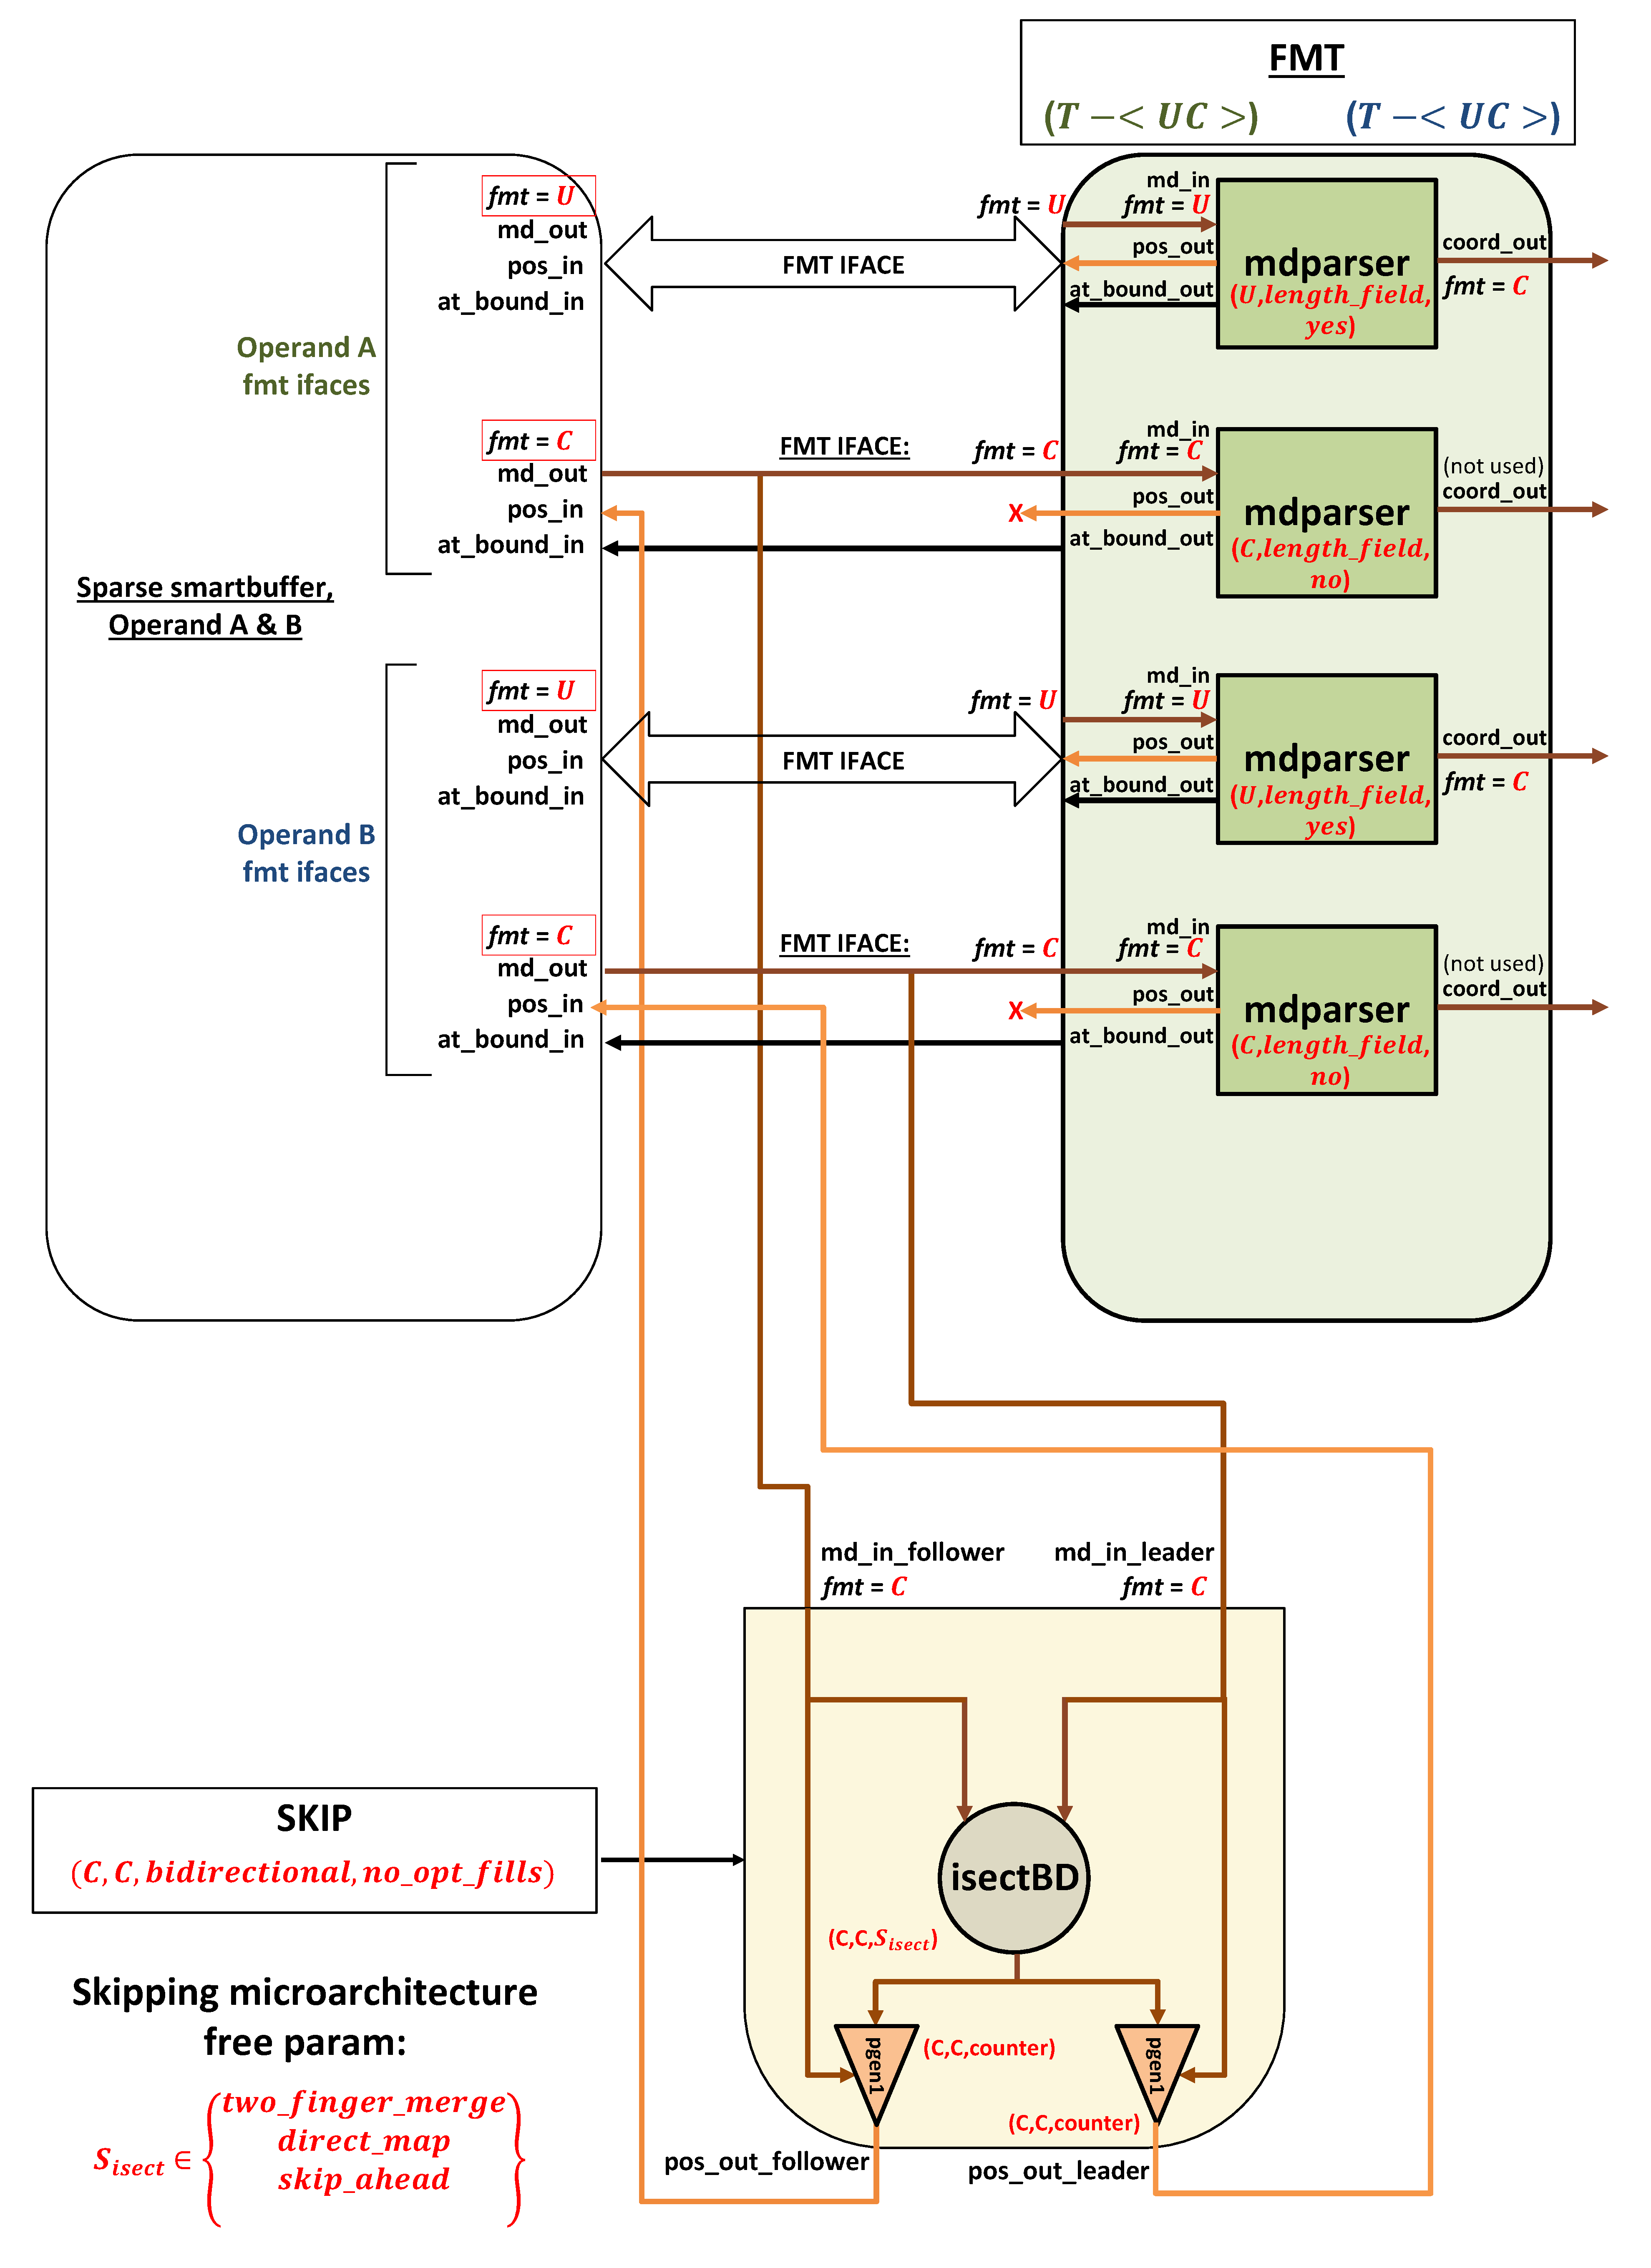
\includegraphics[width=0.7\textwidth]{figures/case_study_inferred_uarch.pdf}
\caption{SAF microarchitecture synthesized by SAFinfer based on declarative specifications.}
\label{fig:case_study_inferred_uarch}
\end{figure}

\clearpage

Figure~\ref{fig:case_study_inferred_uarch} shows the SAF microarchitecture inferred by SAFinfer based on the declarative specifications in the Sparseloop config file. The SAF microarchitecture comprises

\begin{itemize}
    \item A format microarchitecture containing four metadata parsers, one for each rank of each operand fibertree.
    \item A skipping microarchitecture with attributes $(C,C,bidirectional,no\_opt\_fills)$, wired to the format interfaces associated with the two coordinate-payload-format fibers. The skipping microarchitecture comprises a bidirectional intersection unit, as well as two pgen1 units each with attributes $(C,C,counter)$.
\end{itemize}

The bidirectional intersection unit within the skipping microarchitecture has attributes $(C,C,S_{isect})$ where $S_{isect}$ is a free parameter which may be chosen by the user to be either $two\_finger\_merge$ (i.e. ExTensor-like\cite{extensor} naive two-finger merge-like intersection), $direct\_map$ (the direct-mapped intersection unit developed in this work), or $skip\_ahead$ (i.e. ExTensor-like optimized intersection.)

Note that both pgen1 units in the skipping microarchitecture are wired to the format interface pos\_in inputs on the sparse smartbuffer; thus, the output throughput from each pgen1 unit must be be greater-than-or-equal-to the boundary throughput requirement at the corresponding pos\_in inputs, which in turn is a function of the arithmetic throughput as well as the loop nest stride. Thus, as part of an experiment, we can adjust the boundary throughput requirement at pos\_in to reflect what would be required for SIMD 2 arithmetic; SAFmodel scale inference will automatically optimize the skipping microarchitecture to support the necessary throughput.

\subsection{Analysis: skipping microarchitecture design tradeoffs}

\begin{figure}[H]
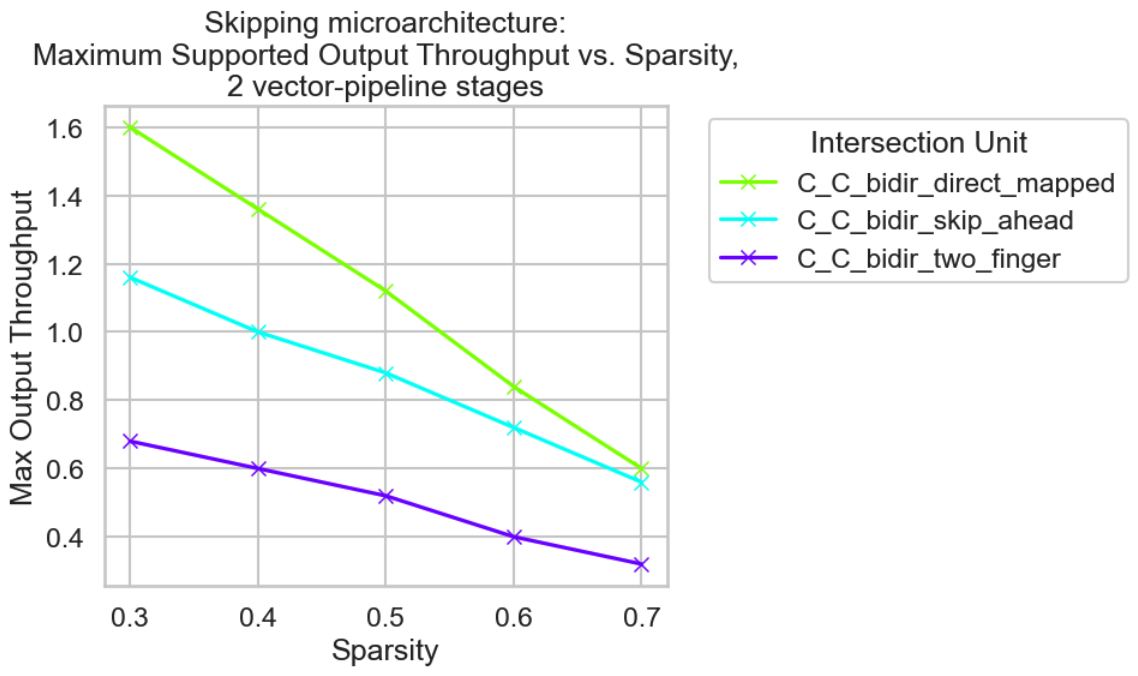
\includegraphics[width=\textwidth]{figures/skip_uarch_pipe_2.png}
\caption{Analysis of intersection unit transfer relations: peak match throughput vs operand sparsity, for intersection units units with two pipeline stages.}
\label{fig:skip_uarch_pipe_2}
\end{figure}

\begin{figure}[H]
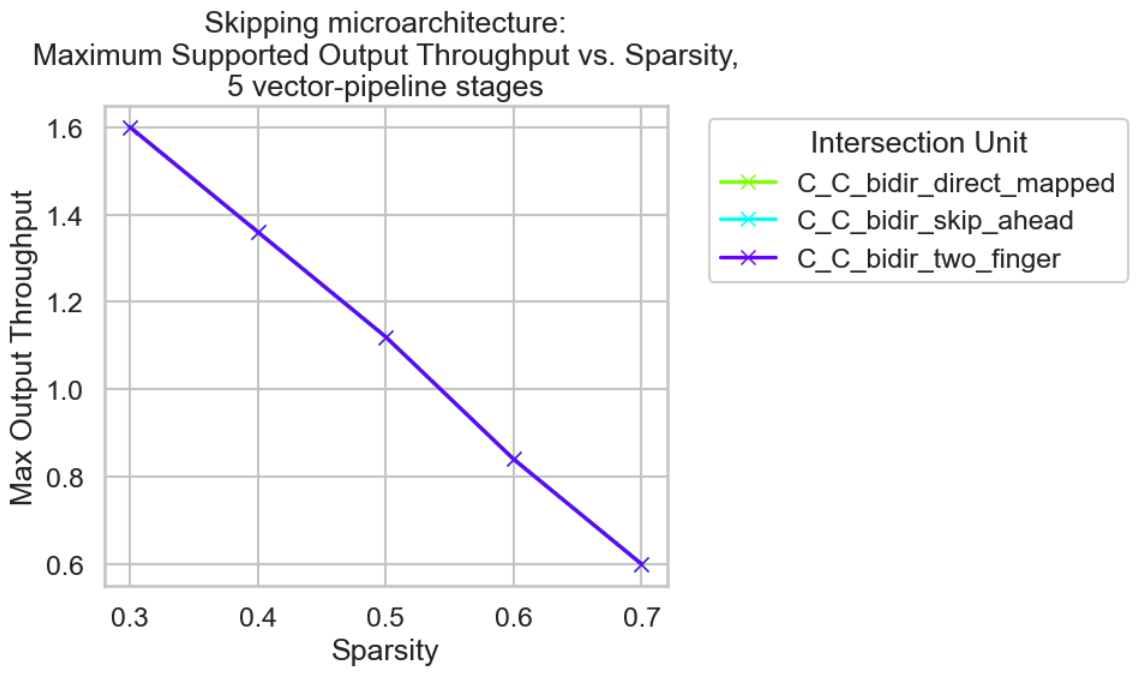
\includegraphics[width=\textwidth]{figures/skip_uarch_pipe_5.png}
\caption{Analysis of intersection unit transfer relations: peak match throughput vs operand sparsity, for intersection units units with five pipeline stages.}
\label{fig:skip_uarch_pipe_5}
\end{figure}

Figures~\ref{fig:skip_uarch_pipe_2} and~\ref{fig:skip_uarch_pipe_5} compare the throughput at the output of the pgen1 units, to the sparsity of the intersection unit input fiber operands, compared between all three intersection unit types for a dense fiber rank size of 16 and a degree-of-vectorization of 4. Figure~\ref{fig:skip_uarch_pipe_2} considers intersection units with 2 pipeline stages while Figure~\ref{fig:skip_uarch_pipe_5} considers intersection units with 5 pipeline stages. 

Note that the relationship between max throughput and sparsity is derived from the transfer relation model that was developed in Section~\ref{sec:c_c_isect_modeling}.

It is clear that pipelining is key to supporting high-throughput intersection, which in turn is critical in a SIMD scenario. It is worth noting that in the scenario shown (vectorization 4, rank size 16), none of these intersection units could supply 2 matches/cycle to support a SIMD 2 arithmetic unit; the max is 1.6 matches/cycle regardless of pipelining. More detailed analysis of the peak matches/cycle throughput supported by each intersection unit variety is provided in Appendix~\ref{appendix:app_intersection_modeling}.

In Figure~\ref{fig:skip_uarch_pipe_2}, direct-mapped intersection attains the highest throughput, followed by skip-ahead intersection unit; this makes sense since direct-mapped intersection has 100\% pipeline efficiency and skip-ahead intersection unit has optimizations to increase pipeline efficiency. This also shows that with 2 pipeline stages, the intersection unit is \textit{efficiency-limited} i.e. limited by how efficient the choice of intersection unit is when it comes to maximizing the number of matches found by a pipeline stage per cycle.

In contrast, in Figure~\ref{fig:skip_uarch_pipe_5}, all intersection units are capable of attaining the same throughput with 5 pipeline stages; this shows that with enough pipeline stages, the intersection unit is \textit{input-rate-limited}, i.e. it is not possible to output more intersections per cycle without changing fiber sparsity, dense rank size, or input vectorization of the intersection unit. Being input-rate-limited is broadly speaking a ``good'' thing, since it means that the particular type of intersection unit we chose is not slowing down the design. We can further observe that while two-finger and skip-ahead intersection unit required multiple pipeline stages in order to be input-rate-limited, direct-mapped intersection unit is already input-rate-limited in Figure~\ref{fig:skip_uarch_pipe_2}. This is because by design, direct-mapped intersection finds all matches in a single cycle, and thus requires only one pipeline stage.

\begin{figure}[H]
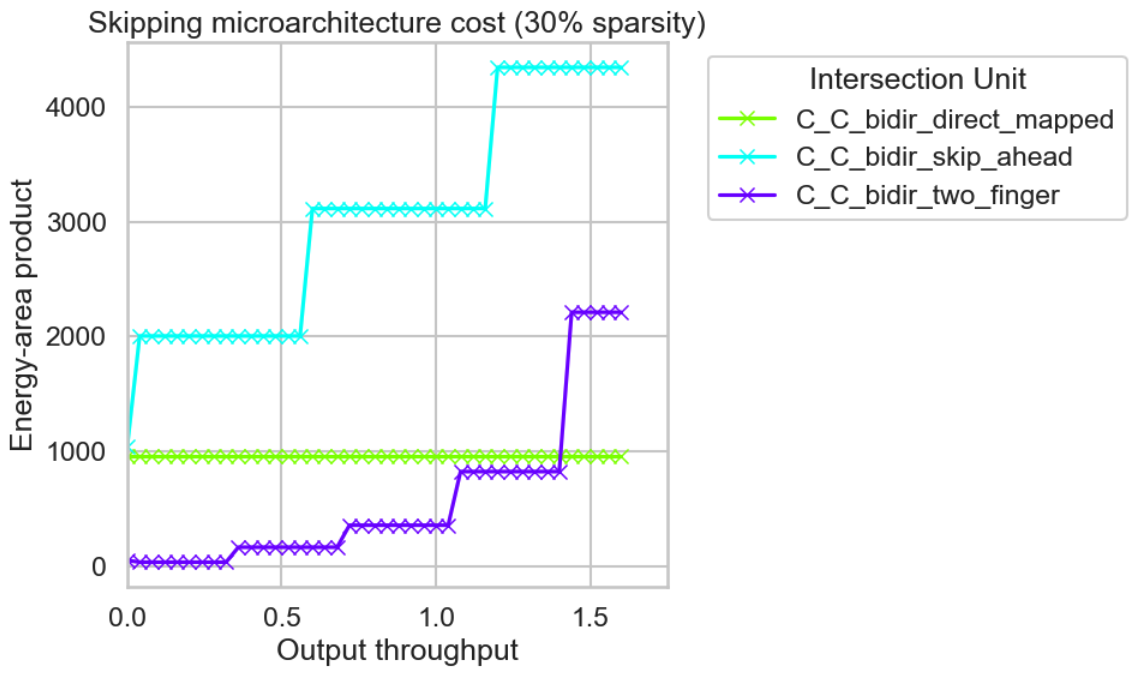
\includegraphics[width=\textwidth]{figures/skip_uarch_sparsity_30pct.png}
\caption{Comparison of energy-per-action/area product for 30\% sparse operands over a range of output throughput requirements.}
\label{fig:skip_uarch_sparsity_30pct}
\end{figure}

\begin{figure}[H]
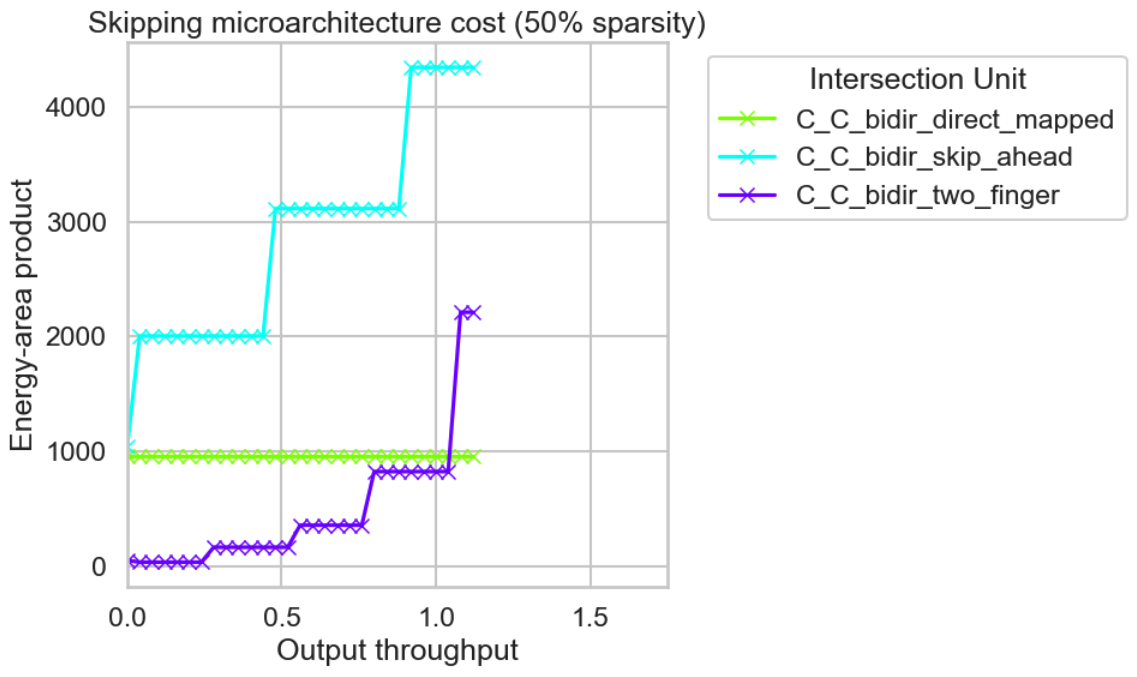
\includegraphics[width=\textwidth]{figures/skip_uarch_sparsity_50pct.png}
\caption{Comparison of energy-per-action/area product for 50\% sparse operands over a range of output throughput requirements..}
\label{fig:skip_uarch_sparsity_50pct}
\end{figure}

\begin{figure}[H]
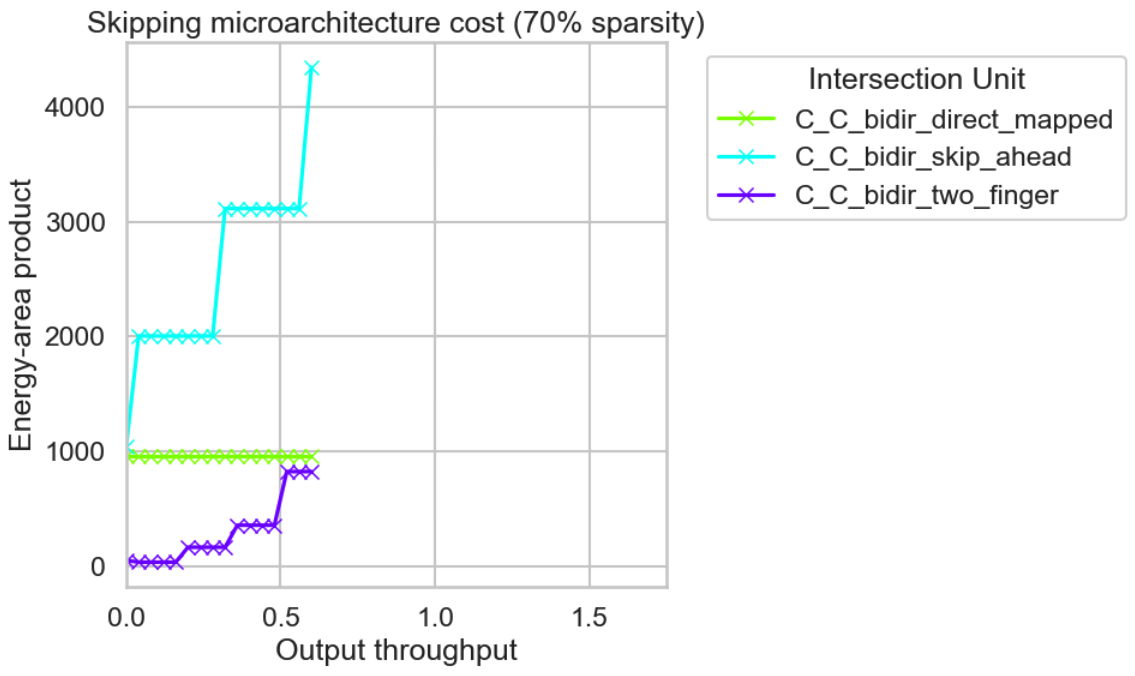
\includegraphics[width=\textwidth]{figures/skip_uarch_sparsity_70pct.png}
\caption{Comparison of energy-per-action/area product for 70\% sparse operands over a range of output throughput requirements..}
\label{fig:skip_uarch_sparsity_70pct}
\end{figure}

Figures~\ref{fig:skip_uarch_sparsity_30pct}, 
~\ref{fig:skip_uarch_sparsity_50pct}, and~\ref{fig:skip_uarch_sparsity_70pct} show how the skipping microarchitecture energy-per-action/area product scales with the output throughput requirement, for each type of intersection unit and for three different sparsity levels. In these figures, the number of pipeline stages is being optimized automatically during scale inference, in order to supply the required throughput. If an intersection unit is not able to supply the requisite throughput with any number of pipeline stages, then the corresponding curve will not have an energy-per-action/area product value associated with that throughput value.

These results suggest that in a SIMD 2 arithmetic scenario, the direct-mapped intersection unit would be a strong candidate for meeting throughput requirement while keeping energy and area low, for the following reasons:

\begin{itemize}
    \item For all sparsities shown, direct-mapped intersection unit has superior energy-per-action/area product \textit{at the highest supported output throughput.}
    \item As shown in Figure~\ref{fig:skip_uarch_pipe_2} Figure~\ref{fig:skip_uarch_pipe_5}, two-finger and skip-ahead intersection unit are efficiency-limited unless they are provisioned with multiple pipeline stages; as shown in Figures~\ref{fig:skip_uarch_sparsity_30pct},~\ref{fig:skip_uarch_sparsity_50pct}, and~\ref{fig:skip_uarch_sparsity_70pct}, this means that the energy-per-action/area product of these intersection units increases substantially with the output throughput design-point. In contrast, direct-mapped intersection unit requires only one pipeline stage regardless of throughput, and thus has uniform energy-per-action and area as the throughput requirement is scaled.
\end{itemize}


Note that in this case study, we are considering intersection units with vector pipelines; however, owing to an early decision to design microarchitecture models based on \textit{combinational unrolling} (Section~\ref{rtl}), the energy-per-action and area characterization results used here are based on combinational unrolling rather than \textit{pipelining}; this means that energy-per-action/area product values quoted in this section may be over-estimates for intersection units with more than one pipeline stage. This could explain the apparent non-linear scaling of two-finger intersection in Figures~\ref{fig:skip_uarch_sparsity_30pct},~\ref{fig:skip_uarch_sparsity_50pct}, and~\ref{fig:skip_uarch_sparsity_70pct}, as combinationally unrolling has non-linear overheads. 

However, it is likely that using energy-per-action and area characterization results based on pipelining, would not significantly change the outcome, because direct-mapped intersection would still have the best pipeline efficiency. Re-running these experiments with models based on pipelining, rather than combinational unrolling, is left for future work.
\chapter{Conclusion}
\label{chapter:conclusion}

A SAF microarchitecture taxonomy was developed and scoped to include format- and skipping- related SAF microarchitectures. A system for inferring low-level scale parameters and automatically sizing SAF microarchitecture components to satisfy workload requirements was also developed.

A library of RTL components was developed and characterized as a basis for creating analytical models of SAF microarchitecture primitives. These RTL models also serve as reference designs.

The SAFTools framework was developed to facilitate the end-to-end process of transforming declarative sparsity optimization specifications (in Sparseloop\cite{sparseloop} format) into SAF microarchitectures, and sizing SAF microarchitecture primitive components to satisfy inferred workload requirements.

A machine-learning method for modeling coordinate-payload bidirectional intersection unit transfer relations was developed, applied, and validated.

A potentially novel intersection unit variety, the direct-mapped intersection unit, was implemented in RTL, characterized, and modeled against other intersection unit varieties. Tentatively, it appears that direct-mapped intersection units may outperform other intersection unit varieties at serving high match throughput in SIMD arithmetic architectures while keeping energy and area low. However, affirming this result is contingent on further refinement of the SAF microarchitecture models developed in this work.

Future work should focus on (1) more in-depth validation of the whole work, (2) refinement of the models, and (3) further experimentation in order to confirm claims about direct-mapped intersection unit. Specific approaches to refining the models could include

\begin{itemize}
    \item Employing layout-level simulation to increase accuracy and capture more subtle overheads such as those resulting from wiring
    \item Where appropriate, implement vector-pipelined \textit{and} combinationall-unrolled variants of each model
    \item Providing options to use different types of pipelining; ensure that all models in a given experiment are configured to use the same form of pipelining.
\end{itemize}

It would be good to see validation and case studies which use Sparseloop alongside SAFTools to inform whole-design decisions.

Note that the full depth of modeling work which was done, was not validated. For example, the impact of clock period on energy and area was considered during characterization, but for brevity was not incorporated into the validation or case-studies.

If the relative benefit of utilizing direct-mapped intersection is supported by future work, this suggests that hashmap-based intersection units suggested in the ExTensor\cite{extensor} are also worth exploring: direct-mapped intersection units are essentially a special case of hashmap-based intersection units, in which the hashmap is the size of the dense rank.
\appendix
\chapter{Explanation of PE area breakdowns from existing sparse tensor accelerator designs}
\label{appendix:pe_breakdowns}

This section justifies the breakdowns of PE area for published sparse tensor accelerator designs, shown in Figure~\ref{fig:saf_uarch_significance}. To keep the analysis as simple as possible, only the PE area is considered.

\section{GAMMA\cite{gamma}}
\label{appendix:pe_breakdowns_gamma}

The GAMMA\cite{gamma} paper quotes the following breakdown of PE area:

\begin{table}
\caption{GAMMA PE area breakdown (Tab. 2 from \cite{gamma})}
\label{tab:gamma_pe_breakdown}
\begin{center}
\begin{tabular}{||l|l|l||}\hline
\textbf{PE subcomponent(s)} & \textbf{PE Area} \%  & \textbf{Categorization based on this work}  \\\hline
Merger	   & 30\% & \textbf{SAF microarchitecture} \\\hline
FP Mul	   & 5.2\% & Architectural compute \\\hline
FP Add	   & 9.4\% & Architectural compute \\\hline
Others	   & 11.1\% & Architectural or non-SAF $\mu$arch \\\hline
\textbf{Total}	   & 100\% & \\\hline
\end{tabular}
\end{center}
\end{table}

Note the lack of an explicit category for PE local memory in the breakdown of Table~\ref{tab:gamma_pe_breakdown}. The breakdown in Table~\ref{tab:gamma_pe_breakdown} can thus be further summarized as

\begin{itemize}
    \item \textbf{SAF microarchitecture:} 30\%, includes merger
    \item \textbf{Compute:} 14.6\%, includes FP Mul and FP Add
    \item \textbf{On-chip memory:} 0\%
    \item \textbf{Other:} 11.1\%
\end{itemize}

which is the breakdown shown in Figure~\ref{fig:saf_uarch_significance}.

\subsection{Relating the Gustavson/row-wise product dataflow to SAF microarchitecture}

The GAMMA PE employs a row-wise product dataflow for loading CSR-format GEMM ($C_{M\times N} = A_{M\times K} \times B_{K\times N}$) operands from memory. A single element $a_{i,j}$ of $A_{M\times K}$ and a row $b_{j,:}$ of $B_{K\times N}$ are loaded from on-chip memory into the PE; this reflects that the $N$ rank of B is traversed in the inner-most loop, while the contracted $K$ rank is traversed at an intermediate loop level. Row-wise product enables a cheap leader-follower skipping microarchitecture because $a_{i,j}$ is guaranteed to be multiplied by all elements of $b_{j,:}$, without needing to do any coordinate-matching (furthermore, the FiberCache\cite{gamma} may be used to support $b_{j:}$ reuse across rows of A.) 

Upon receiving $a_{i,j}$ and $b_{j,:}$ values from memory, the GAMMA PE implements a rank-swap which moves the contracted dimension $K$ into the innermost loop. This enables inner-product accumulation into a single PE output register. The output memory footprint saved by the rank-swap is significant: a design such as MatRaptor\cite{matraptor} which implements row-wise product \textit{without} a rank-swap must store and incrementally accumulate $|K|$ rows of partial outputs, each of size $1 \times |N|$, requiring increased output memory footprint. Given the benefit of rank-swap, is there a tradeoff involved in using it? The use of CSR in GAMMA, means thank rank-swap requires a merge primitive (analogous to the merge operation in mergesort) in order to do a stable sort of multiple $b_{j,:}$ rows based on their rank-$K$ coordinate metadata, effectively implementing a transpose. GAMMA employs a radix-64 merge unit\cite{gamma} in order to do this. 

Although the rank-swap itself is not a sparse optimization, nonetheless the need for this type of merge unit results from employing a rank-swapped dataflow \textit{in the context of employing CSR format for the $B_{K\times N}$ operand}. Thus it is justifiable to say that the merge unit is part of the format microarchitecture which implements the CSR format SAF. It is this format microarchitecture which accounts for 30\% of PE area in GAMMA.

\section{SparTen\cite{sparten}}

The SparTen paper provides the following breakdown of design area:

\begin{table}
\caption{SparTen PE area breakdown (Tab. 4 from \cite{sparten})}
\label{tab:sparten_pe_breakdown}
\begin{center}
\begin{tabular}{||l|l|l||}\hline
\textbf{PE subcomponent(s)} & \textbf{PE Area ($mm^2$)}  & \textbf{Categorization based on this work}  \\\hline
Buffers	   & 0.1 & Architectural memory \\\hline
Prefix-sum	   & 0.418 & \textbf{SAF microarchitecture} \\\hline
Priority Encoder	   & 0.0626 & \textbf{SAF microarchitecture} \\\hline
MACs	   & 0.0432 & Architectural compute \\\hline
Permute network	   & 0.0344 & \textbf{SAF microarchitecture} \\\hline
Other	   & 0.1 & Architectural or non-SAF microarchitecture \\\hline
\textbf{Total}	   & 0.766 & \\\hline
\end{tabular}
\end{center}
\end{table}

Prefix-sum and priority encoder are both key to converting intersected bitmask metadata into memory lookup addresses. The permute network is counted as SAF microarchitecture, on the basis that it is key to SparTen's data orchestration in the presence of sparsity; the permute network helps to address load imbalance.

The breakdown in Table~\ref{tab:sparten_pe_breakdown} can be reduced to

\begin{itemize}
    \item \textbf{SAF microarchitecture:} 67\% (prefix-sum, priority encoder, permute network)
    \item \textbf{On-chip memory:} 13\% 
    \item \textbf{Compute:} 5.6\% (MACs)
    \item \textbf{Other:} 13\%
\end{itemize}

which is the breakdown shown in Figure~\ref{fig:saf_uarch_significance}.

\section{Eyeriss v2\cite{eyerissv2}}

This section justifies the claim in Figure~\ref{fig:saf_uarch_significance} that SAF microarchitecture comprises 7\% of Eyeriss v2 PE area. This claim is not made explicitly in the Eyeriss v2 paper\cite{eyerissv2}; rather, 7\% is an estimate developed in this work, based on metrics that were provided in the paper.

The Eyeriss v2 PE loads activations from the weight scratchpad (weight spad), conditional on the compressed-sparse-column (CSC) metadata of input activation (iact) data being read from the iact spad\cite{eyerissv2}. This pattern of memory accesses can be understood as an $iact \rightarrow weight$ leader/follower skipping SAF. The use of CSC format for weights and iacts can be understood as a $T-<UC>(WH)$ format SAF. \textbf{Note that the use of SAF terminology and sparse tensor notation here is my own interpretation of Eyeriss v2, based on the definitions developed in \cite{sparseloop}\cite{szebook}.}

The leader/follower skipping SAF is lightweight: abstractly, the leader/follower intersection is simply a wire from iact data spad read output to iact address spad read input. Thus for a very rough estimate, the leader/follower intersection area overhead could be quantified as approximately zero. However, in practice there is control logic associated with this abstract wire which adds additional area to the skipping microarchitecture. 

Furthermore, the Eyeriss v2 PE maintains separate address and data memories for each datatype, and data memory is accessed indirectly by first doing a lookup into address memory\cite{eyerissv2}. 

Figure 17 of the Eyeriss v2 paper shows that the PE implements a pipeline for all of these layers of indirect memory access\cite{eyerissv2}. Thus, it is arguable that part of the purpose of the Eyeriss v2 PE pipeline is to implement the leader/follower skipping SAF and the CSC format SAF. For this reason, Figure~\ref{fig:saf_uarch_significance} counts a portion of the PE control logic when estimating the proportion of SAF microarchitecture area in the Eyeriss v2 PE (the iact and weight address buffers are arguably \textit{architectural} overheads required in the implementation of the CSC format SAF, and thus do not count towards SAF \textit{microarchitecture.})



\begin{table}
\caption{Eyeriss v2 PE area breakdown (Fig. 18b from \cite{eyerissv2})}
\label{tab:eyerissv2_pe_breakdown}
\begin{center}
\begin{tabular}{||l|l|l||}\hline
\textbf{PE subcomponent(s)} & \textbf{PE Area} \%  & \textbf{Categorization based on this work}  \\\hline
spad	   & 74.4\% & Architectural memory \\\hline
- \textit{weight data}	   & \textit{21.5\%} &\\\hline
- \textit{weight addr}	   & \textit{5.7\%} & Architectural Format SAF overhead\\\hline
- \textit{iact data}	   & \textit{11.5\%} &\\\hline
- \textit{iact addr}	   & \textit{2.1\%} & Architectural Format SAF overhead \\\hline
- \textit{psum data}   & \textit{33.6\%} &\\\hline
compute (MAC)	   & 5.2\% & Architectural compute \\\hline
I/O FIFOs	   & 9.4\% & Non-SAF-related $\mu$arch\\\hline
control logic	   & 11.1\% & \textbf{Includes SAF $\mu$arch} \\\hline
\textbf{Total}	   & 100.1\% & \\\hline
\end{tabular}
\end{center}
\end{table}

Fig. 18b of the Eyeriss v2 paper\cite{eyerissv2} provides a breakdown of PE area, which is reproduced here in Table~\ref{tab:eyerissv2_pe_breakdown} (\textbf{Note that the categories assigned in the third column are my own interpretation and do not come from the Eyeriss v2 paper}.)

Figure~\ref{fig:saf_uarch_significance} does not count the full 11.1\% of control logic area (shown in Table~\ref{tab:eyerissv2_pe_breakdown}) as SAF microarchitecture. The estimate that SAF microarchitecture accounts for 7\% of PE area is based on examining the PE pipeline and developing a heuristic for the proportion of control logic which is attributable to SAF microarchitecture. The PE pipeline in Fig. 18b of the Eyeriss v2 paper\cite{eyerissv2} shows a five-stage pipeline (ignoring the single architectural register which holds an iact value stationary), and three of these pipeline stages arguably serve to implement SAFs: 

\begin{itemize}
    \item There is a set of pipeline registers between the weight address and weight data spads, and another set of registers between the iact address and iact data spads; since these registers pipeline the process of performing indirect lookups into data memory via lookups into address memory, \textit{here I categorize these two sets of registers as comprising parts of the format microarchitectures for the iact and weight spads.}
    
    \item There is a stage of pipeline registers after the iact spads and before the weight spads; this stage effectively pipelines the process of looking up weights based on iact metadata (i.e. leader/follower skipping), and \textit{therefore I categorize this pipeline stage as being part of the leader/follower skipping microarchitecture.}
\end{itemize}

Fig. 17 from the Eyeriss v2 paper visually suggests that all five pipeline stages are similar in size. Thus, about $\frac{3}{5}$ or 60\% of Eyeriss v2 pipeline area could potentially be categorized as SAF microarchitecture. Extrapolating this 60\% estimate from the pipeline area to the overall control logic area leads to the following estimate for the proportion of SAF microarchitecture area in the PE:

\[(11.1\%\;ctrl\,logic\,area)\times(60\%\;SAF\,\mu arch\,logic)\]

\[ = 6.9\%\; SAF\,\mu arch\,area\]


which is the source of the 7\% claim in Figure~\ref{fig:saf_uarch_significance}. 
\clearpage
\newpage

\chapter{Intersection unit modeling}
\label{appendix:app_intersection_modeling}


\begin{table}
\centering
\caption{Average Cycles Per Intersection}
\begin{tabular}{|c|c|c|c|c|c|c|}
\toprule
 fibLen &  vecLen &  s0 &  s1 &  Direct-mapped &  Naive radix-2 &  Skip-ahead radix-2 \\
\midrule
      4 &       1 & 0.2 & 0.5 &            1.0 &          1.000 &               1.357 \\
      4 &       1 & 0.2 & 0.8 &            1.0 &          1.000 &               1.606 \\
      4 &       1 & 0.5 & 0.8 &            1.0 &          1.000 &               1.497 \\
      4 &       2 & 0.2 & 0.5 &            1.0 &          2.225 &               1.769 \\
      4 &       2 & 0.2 & 0.8 &            1.0 &          1.655 &               1.642 \\
      4 &       2 & 0.5 & 0.8 &            1.0 &          1.580 &               1.700 \\
      4 &       4 & 0.2 & 0.5 &            1.0 &          3.370 &               3.110 \\
      4 &       4 & 0.2 & 0.8 &            1.0 &          2.540 &               2.140 \\
      4 &       4 & 0.5 & 0.8 &            1.0 &          1.630 &               1.850 \\
     32 &       1 & 0.2 & 0.5 &            1.0 &          1.000 &               1.439 \\
     32 &       1 & 0.2 & 0.8 &            1.0 &          1.000 &               1.720 \\
     32 &       1 & 0.5 & 0.8 &            1.0 &          1.000 &               1.614 \\
     32 &       2 & 0.2 & 0.5 &            1.0 &          2.225 &               1.870 \\
     32 &       2 & 0.2 & 0.8 &            1.0 &          2.272 &               1.933 \\
     32 &       2 & 0.5 & 0.8 &            1.0 &          2.248 &               2.027 \\
     32 &       4 & 0.2 & 0.5 &            1.0 &          4.593 &               3.041 \\
     32 &       4 & 0.2 & 0.8 &            1.0 &          4.754 &               2.670 \\
     32 &       4 & 0.5 & 0.8 &            1.0 &          4.930 &               3.080 \\
    256 &       1 & 0.2 & 0.5 &            1.0 &          1.000 &               1.442 \\
    256 &       1 & 0.2 & 0.8 &            1.0 &          1.000 &               1.756 \\
    256 &       1 & 0.5 & 0.8 &            1.0 &          1.000 &               1.658 \\
    256 &       2 & 0.2 & 0.5 &            1.0 &          2.228 &               1.876 \\
    256 &       2 & 0.2 & 0.8 &            1.0 &          2.374 &               1.943 \\
    256 &       2 & 0.5 & 0.8 &            1.0 &          2.385 &               2.037 \\
    256 &       4 & 0.2 & 0.5 &            1.0 &          4.620 &               3.019 \\
    256 &       4 & 0.2 & 0.8 &            1.0 &          5.057 &               2.651 \\
    256 &       4 & 0.5 & 0.8 &            1.0 &          5.115 &               2.945 \\
\bottomrule
\end{tabular}
\end{table}

\newpage

\begin{figure}[H]
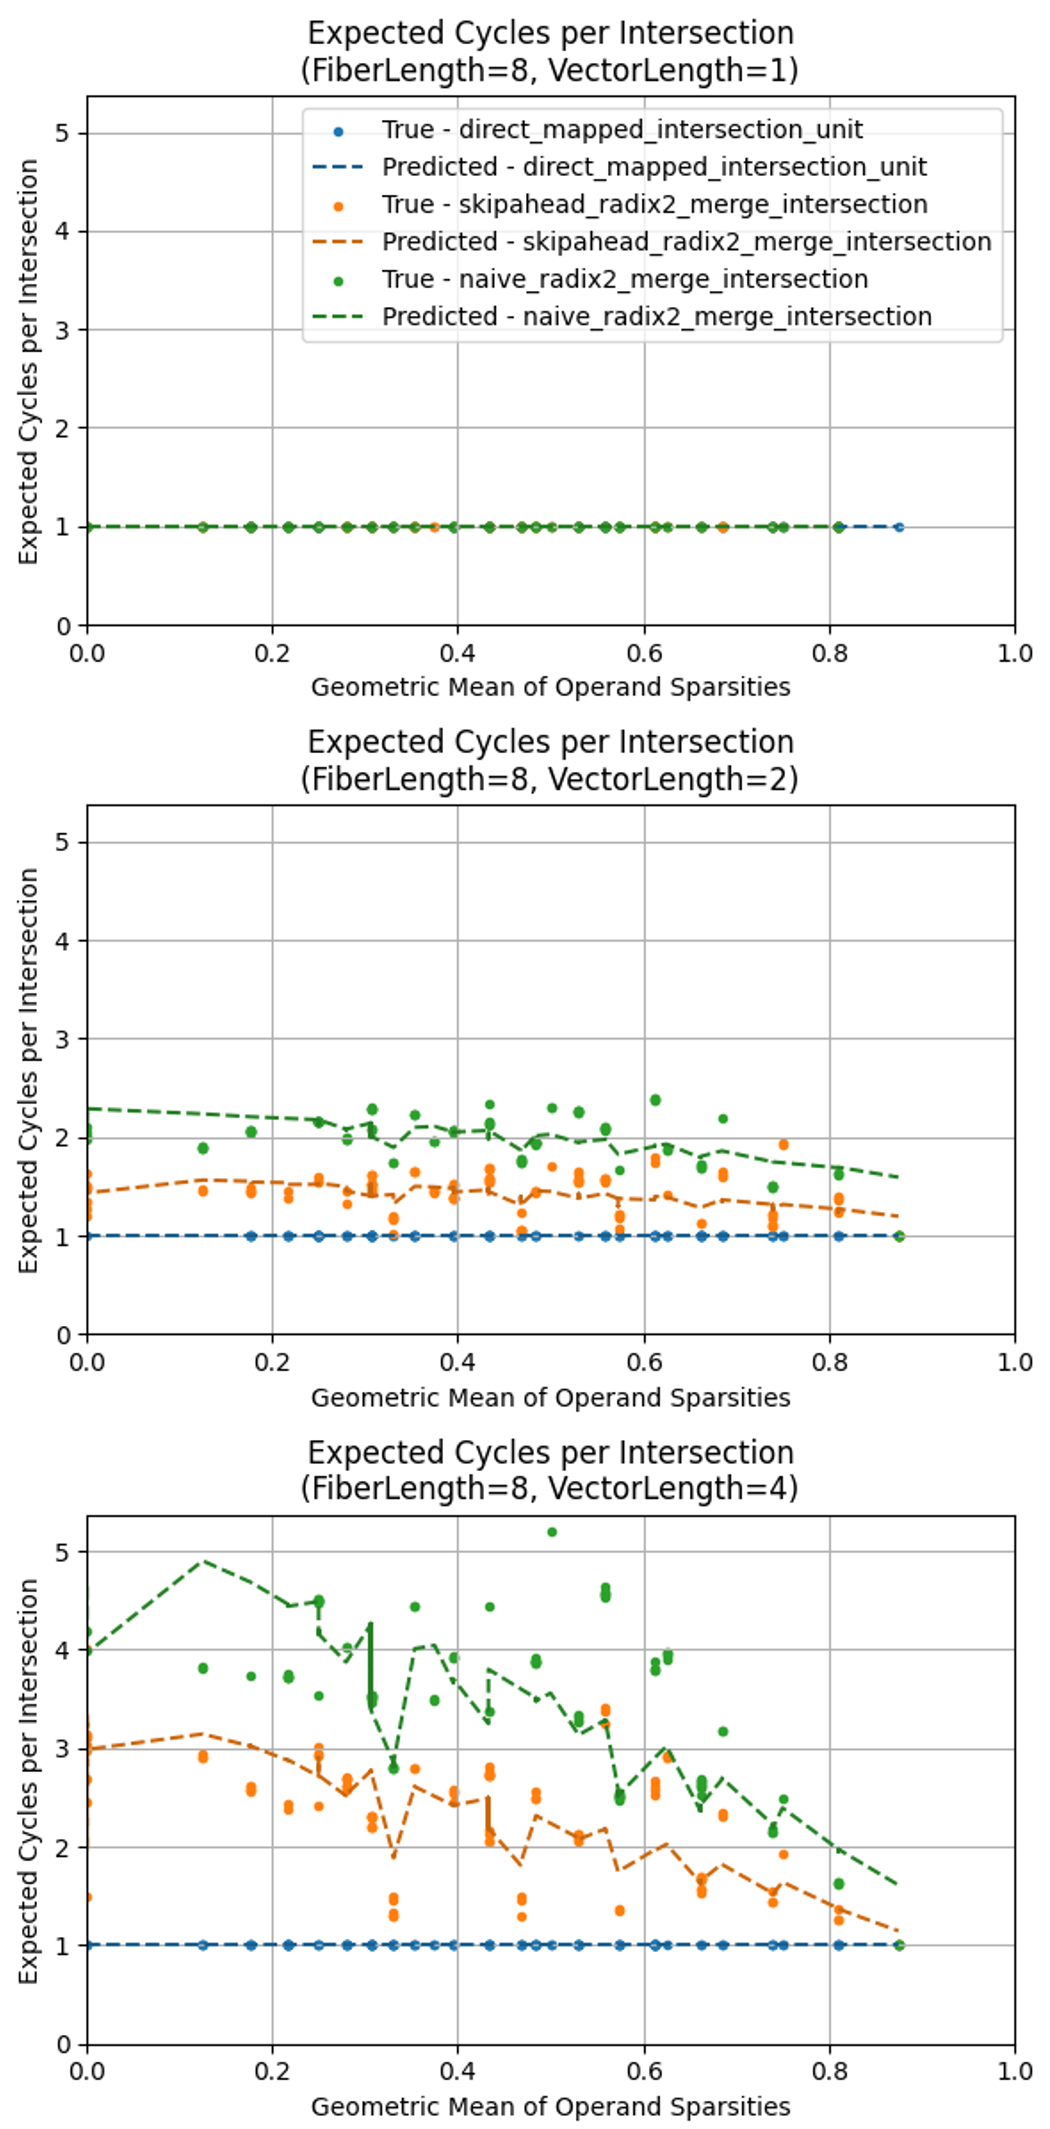
\includegraphics[width=0.75\textwidth]{figures/expected_cycles_F8.png}
\caption{Average cycles-per-intersection when applying a $\{1,2,4\}$-way vectorized intersection unit to intersect two length-8 vectors. Naive two-fingered merge, skip-ahead, and direct-mapped intersection units are compared.}
\label{fig:expected_cycles_F8}
\end{figure}

\newpage

\begin{figure}[H]
\includegraphics[width=0.75\textwidth]{figures/expected_cycles_F16.png}
\caption{Average cycles-per-intersection when applying a $\{1,2,4\}$-way vectorized intersection unit to intersect two length-16 vectors. Naive two-fingered merge, skip-ahead, and direct-mapped intersection units are compared.}
\label{fig:expected_cycles_F16}
\end{figure}

\newpage

\begin{figure}[H]
\includegraphics[width=0.75\textwidth]{figures/expected_cycles_F32.png}
\caption{Average cycles-per-intersection when applying a $\{1,2,4\}$-way vectorized intersection unit to intersect two length-32 vectors. Naive two-fingered merge, skip-ahead, and direct-mapped intersection units are compared.}
\label{fig:expected_cycles_F32}
\end{figure}
\chapter{Worked example: infer SAF microarchitecture topology from architecture and SAFs}
\label{appendix:safinfer_build}

\begin{figure}[ht]
\includegraphics[width=\textwidth]{figures/safinfer_build_00saf.png}
\caption{\textbf{An architectural sparse smartbuffer with format and skipping SAFs.}}
\label{fig:safinfer_build_00saf}
\centering
\end{figure}



\begin{figure}[ht]
\includegraphics[width=\textwidth]{figures/safinference_build_01concretization.png}
\caption{\textbf{An architectural sparse smartbuffer with format and skipping SAFs.}}
\label{fig:safinference_build_01concretization}
\centering
\end{figure}



\begin{figure}[ht]
\includegraphics[width=\textwidth]{figures/safinference_build_02fmtporttype.png}
\caption{\textbf{An architectural sparse smartbuffer with format and skipping SAFs.}}
\label{fig:safinference_build_02fmtporttype}
\centering
\end{figure}



\begin{figure}[ht]
\includegraphics[width=\textwidth]{figures/safinference_build_03fmttopology.png}
\caption{\textbf{An architectural sparse smartbuffer with format and skipping SAFs.}}
\label{fig:safinference_build_03fmttopology}
\centering
\end{figure}



\begin{figure}[ht]
\includegraphics[width=\textwidth]{figures/safinference_build_04mdparserportfmt.png}
\caption{\textbf{An architectural sparse smartbuffer with format and skipping SAFs.}}
\label{fig:safinference_build_04mdparserportfmt}
\centering
\end{figure}



\begin{figure}[ht]
\includegraphics[width=\textwidth]{figures/safinference_build_05mdparserfmtattr.png}
\caption{\textbf{An architectural sparse smartbuffer with format and skipping SAFs.}}
\label{fig:safinference_build_05mdparserfmtattr}
\centering
\end{figure}



\begin{figure}[ht]
\includegraphics[width=\textwidth]{figures/safinference_build_06mdparserstratcust.png}
\caption{\textbf{An architectural sparse smartbuffer with format and skipping SAFs.}}
\label{fig:safinference_build_06mdparserstratcust}
\centering
\end{figure}



\begin{figure}[ht]
\includegraphics[width=\textwidth]{figures/safinference_build_07buffportfmt.png}
\caption{\textbf{An architectural sparse smartbuffer with format and skipping SAFs.}}
\label{fig:safinference_build_07buffportfmt}
\centering
\end{figure}



\begin{figure}[ht]
\includegraphics[width=\textwidth]{figures/safinference_build_08skipportfmt.png}
\caption{\textbf{An architectural sparse smartbuffer with format and skipping SAFs.}}
\label{fig:safinference_build_08skipportfmt}
\centering
\end{figure}



\begin{figure}[ht]
\includegraphics[width=\textwidth]{figures/safinference_build_09skipfmtattrs.png}
\caption{\textbf{An architectural sparse smartbuffer with format and skipping SAFs.}}
\label{fig:safinference_build_09skipfmtattrs}
\centering
\end{figure}



\begin{figure}[ht]
\includegraphics[width=\textwidth]{figures/safinference_build_10skipoptfillscust.png}
\caption{\textbf{An architectural sparse smartbuffer with format and skipping SAFs.}}
\label{fig:safinference_build_10skipoptfillscust}
\centering
\end{figure}



\begin{figure}[ht]
\includegraphics[width=\textwidth]{figures/safinference_build_11skiptopology.png}
\caption{\textbf{An architectural sparse smartbuffer with format and skipping SAFs.}}
\label{fig:safinference_build_11skiptopology}
\centering
\end{figure}

\begin{figure}[ht]
\includegraphics[width=\textwidth]{figures/safinference_build_12isectlfpgenoneopt.png}
\caption{\textbf{An architectural sparse smartbuffer with format and skipping SAFs.}}
\label{fig:safinference_build_12isectlfpgenoneopt}
\centering
\end{figure}

\begin{figure}[ht]
\includegraphics[width=\textwidth]{figures/safinference_build_13foptstratcust.png}
\caption{\textbf{An architectural sparse smartbuffer with format and skipping SAFs.}}
\label{fig:safinference_build_13foptstratcust}
\centering
\end{figure}
%\chapter{Taxoscript syntax}

This section provides a brief overview of the \textit{taxoscript} language that was created for this work and used to develop rewrite rules for the SAFInfer microarchitecture synthesis tool.

\clearpage
\newpage

%\chapter{Modelscript syntax}

This section provides a brief overview of the \textit{modelscript} language that was created for this work and used to develop the SAFModel analytical model library.

\clearpage
\newpage

%% This defines the bibliography file (main.bib) and the bibliography style.
%% If you want to create a bibliography file by hand, change the contents of
%% this file to a `thebibliography' environment.  For more information 
%% see section 4.3 of the LaTeX manual.
\begin{singlespace}
\bibliography{main}
\bibliographystyle{plain}
\end{singlespace}

\end{document}

